%---------------------------------------------------
% University of Sussex thesis template
% Last Edit by Fabrizio Miano, Oct 2017
%---------------------------------------------------
%!TeX root = ../main.tex
\documentclass[a4paper,11pt,oneside,spanish]{memoir}
\usepackage[spanish, es-tabla, es-notilde, es-lcroman, es-nodecimaldot]{babel}


%---------------------------------------------------
% DOCUMENT VARIABLES
% Fill in the lines below to enter your information into the thesis template
% Each of the commands can be cited anywhere in the thesis
%---------------------------------------------------
\newcommand{\myTitle}{My thesis title}
%use surd as ASCII sqrt symbol in case needed and fix title separately

\newcommand{\mySubtitle}{My subtitle}
% Is SUSY in the tau corner? A tale of triggers and tau decays From triggering to taus
%\newcommand{\mySubtitle}{the adventure begins with staus\xspace}
\newcommand{\myDegree}{Doctor of Philosophy \xspace}
\newcommand{\myName}{Francisco \textsc{Sili}\xspace}
\newcommand{\myProf}{Prof. Dr. Maria Teresa \textsc{Dova}\xspace}
\newcommand{\myOtherProf}{Dr. Francisco \textsc{Alonso}\xspace}
\newcommand{\mySupervisor}{Prof. Dr. Maria Teresa \textsc{Dova}\\Dr. Francisco \textsc{Alonso}\xspace}
\newcommand{\myDepartment}{\href{https://www.iflp.unlp.edu.ar/}{Instituto de F\'isica La Plata\xspace}}
\newcommand{\myFaculty}{\href{https://www.exactas.unlp.edu.ar/}{Facultad de Ciencias Exactas\xspace}}
\newcommand{\myUni}{Universidad Nacional de La Plata\xspace}
\newcommand{\myLocation}{La Plata\xspace}
\newcommand{\myTime}{\today\xspace}
\newcommand{\myVersion}{version 0.1\xspace}




\RequirePackage{latex/atlaslatexpath}
\usepackage{latex/packages}
\usepackage{latex/atlasxref_spanish}
\usepackage{definitions}


\graphicspath{{./figures/}} % directory with all the pictures


%---------------------------------------------------
% BEGIN DOCUMENT
%---------------------------------------------------
\begin{document}
% --- to fix figure numbers
\makeatletter
\renewcommand{\counterwithin}{\@ifstar{\@csinstar}{\@csin}}
\makeatother



%---------------------------------------------------
% PREAMBLE: roman page numbering i, ii, iii, ...
%---------------------------------------------------
\pagestyle{custom}% Set page style to custom
\chapterstyle{hansen} % Set chapter style

{
    \frontmatter
    \pagenumbering{roman}
    \clearpage%%%%%%%%%%%%%%%%%%%%%%%%%%%%
%% TITLE PAGE: The title page should give the following information:
%%	(i) the full title of the thesis and the sub-title if any;
%%	(ii) the full name of the author;
%%	(iii) the qualification aimed for;
%%	(iv) the name of the University of Sussex;
%%	(v) the month and year of submission.
\pagestyle{empty}
% \begin{titlepage}
	\begin{center}

		
\includegraphics[height=3.5cm]{UNLP_Logo.png}\\[1.5cm]% \bigskip

		{\LARGE \textsc{\myUni}}\\[0.3cm]
		{\Large \textsc{\myFaculty}}\\[0.3cm]
		{\Large \textsc{\myDepartment}}\\[2cm]

		%\vspace*{.05\textheight}
		\hrule
		{\Large Trabajo de Tesis Doctoral}\\[1cm]
		
		{\Huge \textbf{\myTitle}}\\[1cm] % Thesis title
		{\Huge \textit{\mySubtitle}}\\[0.6cm]
		\hrule

		\vspace{1cm}

		{
			\Large
			Tesista:\\
			% \href{https://www.linkedin.com/in/daniela-koeck-b27041993/}{\myName}
			\myName
		}\\[1.5cm]

		{
			\Large
			Directora: \myProf\\
			Co-Director: \myOtherProf\\
		}

		\vfill
		\large \myLocation, \monthyeardate\today

	\end{center}
% \end{titlepage}

    \clearpage\newpage \vspace*{8cm}
\pdfbookmark[0]{Dedicación}{Dedicación} % Bookmark name visible in a PDF viewer
\thispagestyle{empty}

\begin{flushright}
   % \emph{En memoria de Ayla, que todos los dias me ilumina.}\\
   % \emph{A mis papás y hermano, por su infinito amor.}
\end{flushright}
 % Dedication page
    \clearpage\pagestyle{empty}% Set page style to empty
\pdfbookmark[0]{Agradecimientos}{Agradecimientos} % Bookmark name visible in a PDF viewer
\begin{center}
	\Huge \textsc{\textbf{Agradecimientos}}
	\hrulefill
\end{center}


% Antes que nada pido disculpas a quién no mencioné. Son muchas personas que se me cruzaron estos últimos años. De antemano les agradezco infinitamente a cada uno y todos ustedes.

En primer lugar quiero agradecer a Tere y Fran por la oportunidad que me brindaron de trabajar con ellos, en esta Universidad, y poder cumplir también mi sueño de trabajar en el CERN. Por todo el acompañamiento permanente, por la confianza que tuvieron en mí, por exigirme también cosas que yo no sabía que podía hacer. Sin ese acompañamiento y ayuda esta tesis no hubiera sido posible. 
Gracias Tere también por leer y corregir incontable cantidad de veces esta tesis, no hay Director/a que se dedique tanto a sus estudiantes de Doctorado como vos.

Al grupo de HEP La Plata. Por los almuerzos, las cervezas mensuales, las picadas. Especialmente quiero agradecer a mis compañeros de oficina y amigos Jean y Tomás. Compartir el día a día de este camino con ustedes hizo que todo sea aún más divertido. Por las jodas, risas, cafés, charlas y el estrés que también compartimos. También quiero agradecer Tomás y Fede del grupo de Buenos Aires con quienes compartí oficina, hikes y fiestas.

To all the conveners I had during these 5 years. To the people at EGamma, for their invaluable help and insight on physics. To Jan-Lukas, Nadezda, Ludovica, Ruggero, thanks for all the help I got these years. To the Exotics group, thank you very much Dan, Tamara, Marco, Bing. I can't thank you enough for following my work all these years and helping me every time I asked you. For the long discussions, the round-tables, the presentations, the questions, and your patience with me while I was learning. Thank you very much.

It is impossible to forget thanking all the amazing people I met at CERN. You all made my stays there the most beautiful experiences. To all the people from the UK I met. To Adam, for the countless jokes, the beers at CERN, or everywhere else. To Dani, Marco, Ondrej, for the enormous amount of beers, for the barbecues, dinners, and the friendship that remains every time I go there. To the Tower of the Bear (beer), composed alongside Dani and Fer, for the difficult hike to the Jira, and the not so slippery and snowy hike to Schilthorn. For all the laughs and good times. To Marcelo, not the Marcelo Vieira (football player), but the one who still gets confused for him anyway, haha. Thank you for your friendship all these years since the first afternoon we met at the Saint-Genis Hostel. For all the nightclub nights with the GIA, the dodgy parties you know existed but didn't in the end. The talks, the beers.

Gracias también a Jona y Aimé, que me recibieron con brazos abiertos para cenas, cervezas, juegos y charlas allá en Geneva.

A todos los deadlines, los reales y los que me ponía yo sólo. A las infinitas slides que preparé. A los scripts que me hacen la vida más fácil. A StackOverflow, y más al final a ChatGPT. A las Twikis, que aunque son muy difíciles de encontrar, tienen la información que necesitaba.

A la música, que siempre me acompaña. A los paisajes que vi en Suiza. A los lugares que conocí en Europa.

A mis amigos acá en Argentina. Por las cervezas, los memes, las charlas, por las noches de viceo al conter y al fifa, por las risas.

En mis últimos 15 años también tuve la suerte de compartir la vida con Ayla y Gina, mis dos perritas. También le agradezco a ellas, especialmente a Ayla, que aunque ya no esté siempre me acompaña, en silencio atrás mío, siguiendo cada paso, entendiendo todo. Esta tesis es dedicada a ella, porque me acompaño cuando más yo lo necesitaba, desde mis 12 años hasta mis 27, iluminando siempre mi vida con sus ojos color avellana. A Gina, que con su mirada sincera y fiel está siempre al lado mio.

Pa, Ma, Manu: este trabajo es también dedicado a ustedes, porque ante cualquier cosa de la vida sé que siempre puedo contar con su amor infinito. Gracias por enseñarme a hacerme preguntas, analizar todo y a tener pensamiento crítico. Gracias por las charlas en la mesa en donde siempre aprendo, aunque me hago el que no y que me las sé todas. Gracias por los hermosos días de invierno en la pandemia, haciendo “nesting”. Gracias por ser mis “housemates” durante un poco más de un año… y fueron los mejores! Gracias Pa por ser el mejor compañero de oficina que tuve aunque hablás a los gritos y no sabés conectar los auriculares todavía, jaja. Gracias Ma por estar siempre pendiente de lo que yo necesito, por las infinitas pizzas que comimos y tus datos random en las cenas. Gracias Manu por tu mirada y perspectiva distinta en las cosas de la vida. Aunque no lo creas, aprendo mucho de vos -- igual yo sigo siendo el favorito de Mamá. Gracias a los tres por esas tardes imaginando viajes mirando mapas, hablando un poco sin saber de algunos lugares, pero imaginándonos a los 4 juntos paseando por ahí. Gracias por su paciencia conmigo, por su ayuda, por su amor. Esta tesis es de ustedes como es mía.

Justo antes de venir a La Plata tuve la suerte de conocer a la persona más especial y más buena que conozco. Gracias Abril por estar al lado mío y acompañarme en estos últimos años. Como siempre te lo digo, sos lo mejor que me pasó. Gracias por escucharme, aconsejarme y ayudarme, todo en el camino a ser una mejor persona. Gracias por escuchar cada detalle del análisis y de tratar de entender lo que hago, aunque a veces ni yo puedo. Gracias por venir a visitarme a La Plata, gracias por nuestros viajecitos juntos. Gracias por todo tu amor.

Y a todos de los que me olvido, gracias!



\medskip

{
	\begin{flushright}
		Francisco Sili
	\end{flushright}
} % Acknowledgements page
    % \clearpage%\thispagestyle{empty}
%\pagestyle{custom}% Set page style to custom
\pdfbookmark[0]{Declaration}{declaration} % Bookmark name visible in a PDF viewer

% \begin{center}
% 	\Huge{\textbf{STATEMENT}}
% \end{center}

\vspace*{5cm}

\begin{flushleft}
	\large{\noindent I, \myName, hereby declare that this thesis has not been and will not be, submitted in whole or in part to another university for the award of any other degree.}
\end{flushleft}

\vspace*{2cm}

\begin{minipage}{.45\linewidth}
	\begin{flushleft} %\large
		\textit{\myLocation,} \\
		\textit{\today}% adds space between the two sets of signatures
	\end{flushleft}
\end{minipage}
\hfill
\begin{minipage}{.45\linewidth}
	\begin{flushright} %\large
		\makebox[2.5in]{\hrulefill} \\
		\myName 
	\end{flushright}
\end{minipage}\\ [0.5cm] % Declaration
    \clearpage% % Abstract

\thispagestyle{empty}
\pdfbookmark[0]{Resumen}{Resumen} % Bookmark name visible in a PDF viewer

% \begin{center}
%     %	\bigskip
%     {\normalsize \myUni \\} % University name in capitals
%     {\normalsize \myFaculty \\} % Faculty name
%     {\normalsize \myDepartment \\} % Department name
%     \bigskip\vspace*{.02\textheight}
%     {\Large \textsc{Tesis de Doctorado}}\par
%     \bigskip

%     {\rule{\linewidth}{1pt}\\%[0.4cm]
%     \Large \myTitle \par \mySubtitle} % Thesis title
%     \rule{\linewidth}{1pt}\\[0.4cm]

%     \bigskip
% 	{\normalsize por \myName \par} % Author name
%     \bigskip\vspace*{.06\textheight}
% \end{center}


{\centering\Huge\textsc{\textbf{Resumen}} \par}
\bigskip


En esta tesis se presentan investigaciones originales en física de altas energías con especial énfasis en la búsqueda de nueva física utilizando datos recolectados por el experimento \acs{ATLAS} a partir de colisiones protón-protón del \ac{LHC} a energía de centro de masa de \(\sqs = 13~\TeV\). Estas búsquedas, focalizadas en procesos con estados finales con un fotón y un jet, se llevaron a cabo a partir del desarrollo de estrategias novedosas para la identificación de resonancias provenientes de partículas o de estados de alta masa no incluídos en el \ac{SM}, que se manifiestan como un exceso localizado de eventos sobre el fondo del \ac{SM}. Los resultados obtenidos permitieron establecer los límites más estrictos en la sección eficaz visible de producción de resonancias independiente de modelos así como de resonancias predichas en dos modelos de física más allá del \ac{SM}. Por un lado, para estudiar la elementalidad de los quarks, se consideraron modelos de Quarks Excitados con diferentes acoplamientos (\(f\)) y diferentes sabores, \qstar (\(u^*/d^*\)), \cstar y \bstar, en el que para el caso de \(f = 1\) se excluyeron masas de hasta \(6160\), \(3392\) y \(2469~\GeV\), respectivamente. Cabe destacar que los límites en el modelo de \cstar  corresponden a los primeros resultados obtenidos en estos procesos en los experimentos del \ac{LHC}. Por otro lado, se estudiaron modelos de Micro-Agujeros Negros, como los propuestos por Randall-Sundrum y Arkani-Hamed-Dimopoulos-Dvali que consideran la existencia de una y seis dimensiones extras, respectivamente, para los que los resultados obtenidos permitieron excluir masas de hasta \(5349~\GeV\) y \(7581~\GeV\), respectivamente. A su vez, se realizó un estudio sobre las correcciones a las distribuciones de las variables que describen el pasaje de los fotones por los calorímetros electromagnético y hadrónico -- imprescindibles para la correcta identificación de fotones en el detector \acused{ATLAS}\ac{ATLAS} -- que resultó en una mejora sustancial al método tradicional y se consideró, también, un nuevo enfoque en el que las correcciones se realizan en el nivel más bajo de la reconstrucción de señales en el detector. El desarrollo de este último método resulta de gran interés para la colaboración \ac{ATLAS} en vistas a la utilización de algoritmos de Machine Learning para la identificación de fotones, en particular en el contexto del futuro acelerador High-Luminosity \ac{LHC} (HL-LHC).


\noindent 
 % Abstract page
}



%---------------------------------------------------
% TABLE OF CONTENTS, LISTS OF TABLES & FIGURES
%---------------------------------------------------
{
    \newpage
    % Table of Contents - List of Tables/Figures/Listings and Acronyms

% \refstepcounter{dummy}

\pdfbookmark[0]{\contentsname}{tableofcontents} % Bookmark name visible in a PDF viewer

\setcounter{tocdepth}{2} % Depth of sections to include in the table of contents - currently up to subsections

\setcounter{secnumdepth}{3} % Depth of sections to number in the text itself - currently up to subsubsections

% \manualmark
% \markboth{\spacedlowsmallcaps{\contentsname}}{\spacedlowsmallcaps{\contentsname}}
\tableofcontents
% \automark[section]{chapter}
% \renewcommand{\chaptermark}[1]{\markboth{\spacedlowsmallcaps{#1}}{\spacedlowsmallcaps{#1}}}
% \renewcommand{\sectionmark}[1]{\markright{\thesection\enspace\spacedlowsmallcaps{#1}}}

\clearpage
\begingroup 
    \let\clearpage\relax
    \let\cleardoublepage\relax
    \let\cleardoublepage\relax

    %----------------------------------------------------------------------------------------
    %	List of Figures
    %----------------------------------------------------------------------------------------

    % \refstepcounter{dummy}
    % \addcontentsline{toc}{chapter}{\listfigurename} % Uncomment if you would like the list of figures to appear in the table of contents
    \pdfbookmark[1]{\listfigurename}{lof} % Bookmark name visible in a PDF viewer

    \listoffigures

    \vspace{8ex}
    \newpage

    %----------------------------------------------------------------------------------------
    %	List of Tables
    %----------------------------------------------------------------------------------------

    % \refstepcounter{dummy}
    % \addcontentsline{toc}{chapter}{\listtablename} % Uncomment if you would like the list of tables to appear in the table of contents
    \pdfbookmark[1]{\listtablename}{lot} % Bookmark name visible in a PDF viewer

    \listoftables

    \vspace{8ex}
    \newpage

    %----------------------------------------------------------------------------------------
    %	List of Listings
    %---------------------------------------------------------------------------------------- 

    % \refstepcounter{dummy}
    % %\addcontentsline{toc}{chapter}{\lstlistlistingname} % Uncomment if you would like the list of listings to appear in the table of contents
    % \pdfbookmark[1]{\lstlistlistingname}{lol} % Bookmark name visible in a PDF viewer

    % \lstlistoflistings 

    % \vspace{8ex}
    % \newpage

    %----------------------------------------------------------------------------------------
    %	Acronyms
    %----------------------------------------------------------------------------------------

    % \refstepcounter{dummy}
    % %\addcontentsline{toc}{chapter}{Acronyms} % Uncomment if you would like the acronyms to appear in the table of contents
    % \pdfbookmark[1]{Acronyms}{acronyms} % Bookmark name visible in a PDF viewer

    % \markboth{\spacedlowsmallcaps{Acronyms}}{\spacedlowsmallcaps{Acronyms}}

    % \chapter*{Acronyms}

    % \begin{acronym}[UML]
    % \acro{DRY}{Don't Repeat Yourself}
    % \acro{API}{Application Programming Interface}
    % \acro{UML}{Unified Modeling Language}
    % \end{acronym}
\endgroup
}




%---------------------------------------------------
% MAIN THESIS TEXT: arabic page numbering 1, 2, 3, ...
% THESIS CONTENT - CHAPTERS
%---------------------------------------------------
\mainmatter
\pagenumbering{arabic}






% Possible quotes for chapters



% “Not only is the Universe stranger than we think, it is stranger than we can think.” Werner Heisenberg

% "Any sufficiently advanced technology is indistinguishable from magic." Arthur C. Clarke
% “Experiment is the sole judge of scientific truth.” Richard Feynman

% “There is a single light of science, and to brighten it anywhere is to brighten it everywhere.” Isaac Asimov
% “Nothing in life is to be feared, it is only to be understood. Now is the time to understand more, so that we may fear less.” Marie curie

% “There is a crack in everything. That's how the light gets in.” Leonard Cohen
% “If you wish to make an apple pie from scratch, you must first invent the universe.” Carl Sagan
% “I don't want to believe. I want to know.” Carl Sagan
% “If I have seen further it is by standing on the shoulders of Giants.” Isaac Newton
% "Only those who will risk going too far can possibly find out how far one can go." T. S. Elliot
% “Somewhere, something incredible is waiting to be known.” Carl Sagan



\acresetall
\chapter*{Introducci\'on}
\addcontentsline{toc}{chapter}{Introducci\'on}
\markboth{}{Introducci\'on}

This thesis presents a search for new phenomena in high-mass final states with a photon and a jet in proton-proton (\pp) collisions at a centre-of-mass energy of 13 TeV using data collected by the \acs{ATLAS} detector. \acs{ATLAS} (“A Toroidal LHC ApparatuS”) is one of the two general-purpose detectors at the Large Hadron Collider (\acs{LHC}) and the biggest multi-purpose particle detector ever built. It is used to investigate a wide range of physics, from Standard Model (\acs{SM}) measurements, such as precision tests of quantum chromodynamics or study of the properties of the Higgs boson, to the search of new phenomena like extra dimensions and dark matter candidates. The LHC, built by the European Organization for Nuclear Research (\acs{CERN}) and installed in a 27-kilometre circular tunnel, is the world's largest and most powerful particle collider. This machine is capable of colliding energetic beams of protons (or heavier nuclei) at rates upward of millions per second. The precision and high beam energy of the LHC allow to explore the tera-electronvolt scale, an energy range never before achieved in a particle collider.



The thesis is divided into three parts. The first part describes the theory background and motivations of the work, in which the first chapter describes the Standard Model (SM) showing the excellent agreement there is between the theory and the experimental data. It also shows the actual problems of the SM, which motivates the search for New Physics.

The second part describes the experiment. CHAPTER describes the ATLAS experiment, with each sub-detector in detail, to finally describes how the samples for data analysis are produced. The reconstruction of the different physics objects is explained in CHAPTER. At the end of the second part, a special chapter is dedicated to the photon identification, where a new method for correcting the shower shapes is explained and detailed.

The third part of the thesis is dedicated to the photon+jet resoanance search.
In CHAPTER, the general strategy and motivation of the search is discussed. The samples generation is discussed in CHAPTER, where the final event selection is given in CHAPTER.
The methods for the background estimation as well as background modeling is given in CHAPTER AND CCHAPETER.
The systematic uncertainties are discussed in CHAPTER, and finally in CHAPTER and CHAPTER, the statistical analysis with the results are shown.

Finally, the conclusions of the work are present in CHAPTER.


%\epigraph{\emph{The journey, not the destination matters.}}{Thomas S. Eliot}


%Provide preliminary background information that puts your research in context (Why?)
%
%Clarify the focus of your study (What?)
%
%Point out the value of your research(including secondary research)!! (What gain?)
%
%Specify your specific research aims and objectives 

%The reader needs to know why your research is worth doing


%maybe want to motivate why looking at run-2 data? 

%At the time of writing
%between run 2 and run 3
%at time of writing,  run-3 data-taking is just about to start.. 
%important to use previous dataset to gauge limitations of searches
%--> crucial to contribute to the overall runnning of the experiment
%--> study and understand trigger 
%The result is striking. Two --> WIMP miracle!
%seemingly unrelated problems – the Higgs unnaturalness (rooted in the quantum structure
%of the particle world at distances of 10−20 meters and below) and the nature of dark matter
%(observed from galactic distances of 1020 meters to the largest scales in the universe)
%the science historian Thomas Kuhn
%We are confronted with the need to reconsider the guiding principles that have been used for decades to address the most fundamental questions about the physical world. These are symptoms of a phase of crisis.
%Greek krisis, which means “decisive moment”, “turning point”,
%privilege of the opportunity for an upcoming paradigm change.

% Within the last decades of particle physics research there have been many milestones and discoveries, narrowing in on the building blocks of matter and leading to the development of the Standard Model (\acs{SM}) of particle physics as we know it today. 
% This has been achieved through extraordinary efforts and interplay between experimental measurements unravelling hints and evidence of new particles,  and theoretical effort of tying this to an overarching theory and achieving more precise predictions:
% from the discovery of the electron in 1897 \cite{ElectronThomson},  to the discovery of the tau lepton in 1975 \cite{TauDiscovery},  to the most recent success of the theoretical predictions lying in the experimental discovery of the Higgs boson \cite{ATLASHiggsDiscovery,CMSHiggsDiscovery}.  In the last ten years since the Higgs boson's discovery,  its properties have been measured to high precision \cite{HiggsReviewATLAS10years} and the Standard Model’s predictions have been put to stringent tests. 
% In various measurements, tensions with predictions of the Standard Model have been appearing, hinting towards a larger underlying theory. The limitations of the Standard Model have become more and more evident. The Hierarchy problem,\cite{SUSYPrimer}, questioning the difference in scales between the Higgs mass and the Planck scale, raising the need for unnatural fine-tuning, is only one of the hints for the need for a larger principle. The evolution of our universe into a matter-dominated universe is so far unexplained, with no mechanisms within the Standard Model to sufficiently generate this asymmetry with anti-matter \cite{WMAP, Thomson,Sakharov}. Lastly, one of the most striking hints connects the limitations of the theoretical model describing the smallest building blocks in our universe to the largest structures known to humankind. The presence of Dark Matter \cite{Zwicky,RubinKent,RotationCurves,Planck,BulletCluster, OtherMergingClusters} in galaxies and galaxy clusters can not be explained through a composition of Standard Model particles. 

% An additional symmetry between bosons and fermions called \ac{SUSY} could offer solutions to many of these limitations. Not only could \ac{SUSY}  avoid the need for fine-tuning of the Higgs mass, but also \acp{WIMP} predicted by SUSY could make up a component of Dark Matter. This striking connection of two problems at length scales varying from the size of a fundamental particle to galaxies and galaxy clusters is known as the WIMP miracle. \\
% Supersymmetric particles have been searched for in many ways at the Large-Electron-Positron collider, the Large-Hadron-Collider as well as through a variety of non-collider experiments. Up to the moment of writing this thesis, there has been no direct detection of Dark Matter particles and no evidence of supersymmetric particles at colliders. 

% According to definitions of science historian Thomas Kuhn and discussion thereof of Gian Francesco Giudice (\cite{Kuhn,Giudice}) particle physics can currently be described to be in a period of "krisis".  Krisis has to be understood in its original meaning - a period of change and anticipation. This period can be frustrating and confusing, with a lack of direction to a new underlying principle,  but should be seen as a privilege.  A period preceding a paradigm change,  with room for creativity for new ideas but also the need for diligent exploration of limitations in current experiments.

% At the time of writing, a new data-taking period at the LHC has just begun. In preparation for this new data taking, it is crucial to thoroughly analyse the Run-2 data set, find its limitations and uncovered areas of new physics searches in order to prepare for the new challenges to come. 

% In this thesis, a search for \ac{SUSY} has been performed, looking for a production of the lightest chargino and next to lightest neutralino (supersymmetric partners of SM gauge bosons), decaying via a scalar tau lepton into a final state with hadronically decaying tau leptons. This search has been performed with data collected by the ATLAS detector at the LHC, as part of the ATLAS Collaboration. This final state with hadronically decaying tau leptons belongs to the ‘paths less walked’ within the ATLAS Collaboration, due to its challenging reconstruction. This offers an interesting window to determine and overcome the limitations of the ATLAS Collaboration’s search program for \ac{SUSY}. This analysis has been the author’s full responsibility. 
% Next to this main effort within this thesis, the performance of electron triggers within ATLAS have been studied as part of the author's qualification task as well as continued commitment to ensure the successful operation and good performance of ongoing ATLAS data-taking.

% The structure of this thesis is as follows: A brief overview of the theoretical concepts of the SM as well as its limitations,  motivating \ac{SUSY} is given in Chapter \ref{ch:theory}. This is followed by a conceptual description of LHC proton-proton collisions and the ATLAS detector in chapter \ref{ch:expsetup}. Further details on the data collection and reconstruction of collision events as well as the simulations used to study the events is given in Chapter \ref{ch:DAQ}. A detailed view on the electron trigger and its performance is given in Chapter \ref{ch:trigger}. The search for supersymmetric gauge bosons in all its necessary details is given in Chapter \ref{ch:analysis}. 
\acresetall


\part{Motivación Teórica}
\label{part:theory}
\chapter{Motivación teórica}
\label{ch:theory}
\epigraph{\emph{\enquote{Not only is the Universe stranger than we think, it is stranger than we can think.}}}{Werner Heisenberg}


Esta tesis se centra en la búsqueda de nuevas partículas predichas por diferentes escenarios más allá del \ac{SM}. En este capítulo se presenta un resumen de los principales conceptos del \ac{SM} utilizados a lo largo de esta tesis. Además, se describen las interacciones hadrónicas en una colisión \pp y en el proceso de producción de fotones \textit{prompt}.
A continuación, en \Sect{\ref{sec:theory:bsm}} se ofrece una vista general de las limitaciones actuales del \ac{SM} y cómo, con modelos de física \ac{BSM}, se pretenden resolver estos problemas.
Por último, en la \Sect{\ref{sec:theory:mc_simulation}}, el capítulo termina con cómo se simulan estos procesos del \ac{SM} utilizando \ac{MC}, mostrando los diferentes pasos y herramientas para hacerlo.




\section{El Modelo Estándar}
\label{sec:theory:sm}

El \acf{SM} de física de partículas es la teoría matemática que describe todas las partículas elementales conocidas y sus interacciones.
La teoría se ha ido desarrollando a lo largo de varias décadas y tras numerosos experimentos que respaldaron sus predicciones, se ha convertido en la teoría más completa de la física de partículas.

El \ac{SM} logra describir tres de las cuatro fuerzas fundamentales de la naturaleza: las interacciones \ac{EM}, débil y fuerte, las cuales actúan en distintos rangos.
La gravedad, la cuarta fuerza de la naturaleza, aunque no está incluida en el \ac{SM}, es la más débil de las interacciones y tiene un alcance infinito.
Las tres fuerzas fundamentales del \ac{SM} resultan del intercambio de partículas que pertenecer al grupo de \textit{bosones}. Las partículas de materia, los \textit{fermiones}, interactúan entre ellas transfiriendo cantidades discretas de energía a través del intercambio de estos bosones.



\subsection{Partículas elementales y sus interacciones}
\label{subsec:theory:sm:particles_interaction}

Según el \ac{SM}, toda la materia está formada por fermiones, que son partículas que siguen la estadística de Fermi-Dirac y tienen spin semi-entero. Estos fermiones interactúan entre sí mediante el intercambio de bosones, que son partículas de spin entero, siguiendo la estadística de Bose-Einstein. Hasta la fecha no ha habido ningún experimento capaz de encontrar pruebas de que estas partículas tengan estructura interna.

\begin{figure}[ht!]
    \centering
    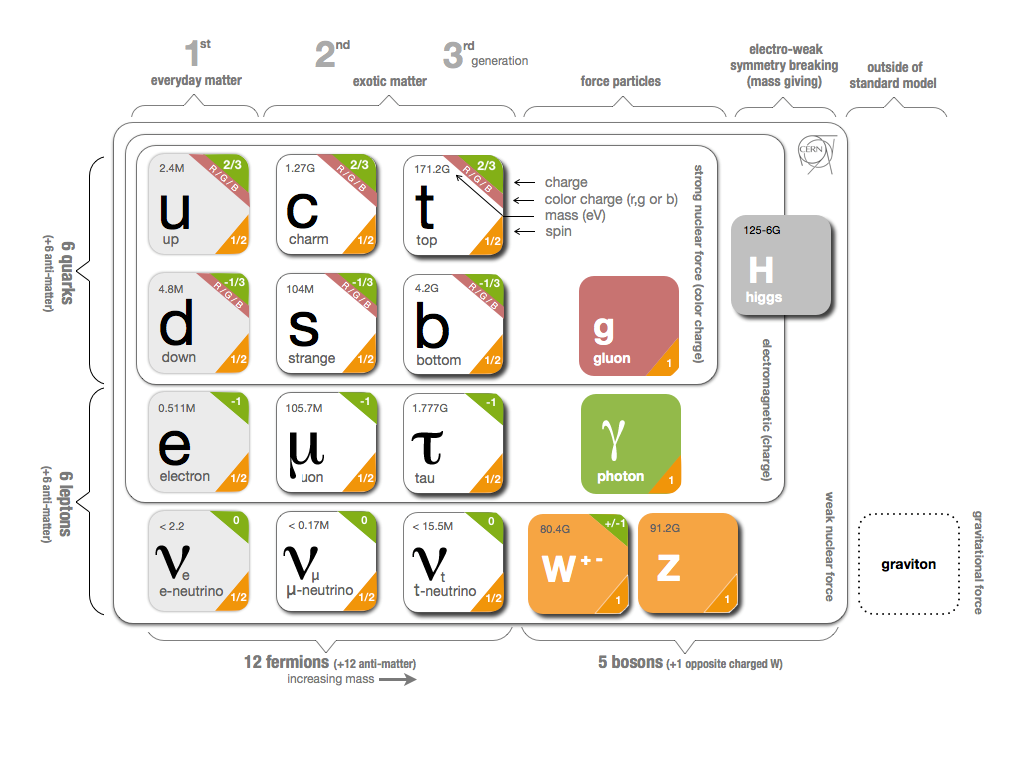
\includegraphics[width=\linewidth]{2_theory/sm}
    \caption{Partículas del \ac{SM} y sus propiedades. Todos los fermiones participan en la interacción débil, pero sólo los quarks interaccionan con los gluones, mientras que tanto los quarks como los leptones cargados interaccionan mediante la fuerza \ac{EM}. Los neutrinos, al ser neutros e incoloros, sólo interaccionan con los bosones \Wboson y \Zboson a través de la fuerza débil. Por último, el gravitón, aunque aún no se ha descubierto, debería ser el correspondiente portador de la fuerza gravitatoria. Extraído de la \Refn{\cite{SM_diagram}}.}
    \label{fig:theory:sm:particles_interaction:particles}
\end{figure}

Los fermiones se dividen en dos tipos de partículas elementales: los leptones y los quarks. Existen seis leptones clasificados según su carga que se dividen en tres familias o generaciones, ordenadas en función de su masa. Las partículas de las generaciones superiores tienen mayor masa y son muy inestables, decayendo en leptones de generaciones inferiores. Por esta razón, la materia se construye a partir de leptones de primera generación. Los leptones son: electrón (\(e\)), muón (\(\mu\)) y tau (\(\tau\)), con sus respectivos neutrinos: neutrino electrón (\(\nu_{e}\)), neutrino muón (\(\nu_{\mu}\)) y neutrino tau (\(\nu_{\tau}\)).
También hay seis antileptones que tienen carga eléctrica opuesta a la de los leptones. El electrón, el muón y el tau tienen carga eléctrica y una masa considerable, mientras que los neutrinos son eléctricamente neutros y tienen una masa muy pequeña (aunque en el \ac{SM} es estrictamente cero).

Del mismo modo, hay seis sabores (flavours) de quarks, también con sus respectivas antipartículas: up (\(u\)), down (\(d\)), charm (\(c\)), strange (\(s\)), top (\(t\)) y bottom (\(b\)). Los quarks también presentan otra propiedad que es el número cuántico de color y sólo se mezclan de tal manera que forman objetos sin color. En la \Fig{\ref{fig:theory:sm:particles_interaction:particles}} se muestra un resumen de los quarks y sus propiedades.


Cada una de las tres fuerzas en el \ac{SM} se describe mediante una \ac{QFT}.
La fuerza fuerte, mediada por gluones sin masa, es responsable de la interacción entre los quarks que aunque no tienen carga eléctrica poseen carga de color. A pesar de que estos no tienen masa, la interacción fuerte se hace más fuerte a bajas energías, confinando quarks y gluones dentro de hadrones debido a la propiedad de libertad asintótica y a la propiedad de \textit{confinamiento}, las cuales serán discutidas más adelante.
La fuerza \ac{EM} entre partículas cargadas está mediada por fotones. Los fotones no tienen masa y, en consecuencia, la interacción tiene un alcance infinito.
Por último, la interacción débil está mediada por los bosones masivos \Wboson y \Zboson, que dan lugar a interacciones de corto alcance. Las propiedades fundamentales de estos bosones también se muestran en la \Fig{\ref{fig:theory:sm:particles_interaction:particles}}.









\subsection{Breve descripción matemática del Modelo Estándar}
\label{subsec:theory:sm:mathematical}

El \ac{SM} es una teoría de campos renormalizable basada en simetrías locales que proporciona una descripción de las partículas fundamentales y sus interacciones: la fuerte, la débil y la \ac{EM}. Estas interacciones aparecen por el requisito de que la teoría es invariante bajo transformaciones gauge locales del grupo de simetría:
\begin{equation*}
    SU(3)_{C} \times SU(2)_{L} \times U(1)_{Y},
\end{equation*}
donde \(Y\) es la hipercarga, \(L\) la helicidad izquierda y \(C\) la carga de color, y representan las cantidades conservadas del grupo de simetría. Cada transformación gauge local puede ser absorbida dentro de un campo de gauge, con las excitaciones de los campos gauge llamadas bosones gauge. El sector \ac{EW} del \ac{SM} \(SU(2)_{L} \times U(1)_{Y} \to U(1)_{\text{EM}}\) describe las interacciones débil y \ac{EM}, tras el mecanismo de ruptura espontánea de simetría en virtud del potencial de Higgs. El grupo no abeliano \(SU(3)_C\), con carga de color, describe las interacciones fuertes entre quarks y gluones y la teoría se conoce como \ac{QCD}~\cite{Ellis-1996-book}.

En principio, las partículas incluidas en el \ac{SM} carecen de masa a diferencia de las partículas observadas en la naturaleza. Aunque las ecuaciones de la interacción \ac{EW} describen correctamente partículas como el fotón, no dan cuenta de las masas de los bosones \Wboson y \Zboson. Para solucionar este problema se introdujo el concepto de \ac{EWSB}, conocido como mecanismo de Brout-Englert-Higgs~\cite{Higgs-1964_1,Higgs-1964_2,Higgs-1966,Englert_Brout-1964}. Este mecanismo explica cómo los bosones \Wboson y \Zboson adquieren masa a través de la ruptura espontánea de la simetría \ac{EW}, causada porque el campo escalar de Higgs adquiere un \ac{VEV} distinto de cero. Además, predice la existencia de una nueva partícula escalar, dando lugar a un nuevo bosón masivo de spin 0, denominado bosón de Higgs. Esta partícula fue confirmada experimentalmente en 2012 por las colaboraciones \ac{ATLAS}\acused{ATLAS} y \ac{CMS}\acused{CMS} en el \ac{LHC}\acused{LHC}, con una masa medida de \(125.11 \pm 0.11~\gev\)~\cite{ATLAS-HiggsObservation,CMS-HiggsObservation,ATLAS-Higgs-2024}.








\subsubsection{The interaccón \acl{EW}}

Las interacciones \ac{EW} satisfacen la simetría de gauge del grupo \(SU(2)_L \times U(1)_Y\). El grupo \(SU(2)_L\), llamado isospín débil actúa sólo sobre los fermiones de quiralidad izquierda y \(U(1)_Y\) es el grupo de hipercarga que actúa sobre ambas quiralidades de forma vectorial.
El grupo \(SU(2)_L \times U(1)_Y\) tiene cuatro generadores, de los cuales tres pertenecen al isospín débil: \(T_i = \frac{\sigma_i}{2}\), siendo \(i = 1,\, 2,\, 3\) y \(\sigma_i\) las matrices de Pauli y uno al grupo de hipercarga: \(\frac{Y}{2}\). Los fermiones izquierdos se transforman como dobletes bajo \(SU(2)_L\), \(f_L \ra e^{i T_i \theta_i} f_L\) con
\begin{equation}
    f_L = \mqty( \nu_L\\ e_L ), \mqty( u_L\\ d_L ), \dots,
\end{equation}
mientras que los fermiones derechos se transforman como singletes \(f_R \ra f_R\) con
\begin{equation}
    f_R = e_R, \, u_R,\, d_R, \dots.
\end{equation}
Esta distinción entre izquierdos y derechos implica que la teoría \(SU(2)_L \times U(1)_Y\) es una teoría quiral.
Por otro lado, la carga eléctrica está relacionada con la tercera componente del isospín débil \(T_3\) y la hipercarga \(Y\), según la fórmula de Gell-Mann Nishijima:
\begin{equation}
    Q = T_3 + \frac{Y}{2}
\end{equation}

El número de bosones de gauge asociados coincide con el número de generadores del grupo de simetría. Para el isospín débil hay 3 bosones \(SU(2)_L\): \(W_{\mu}^1,\, W_{\mu}^2,\, W_{\mu}^3\), y para \(U(1)\) se tiene un bosón de hipercarga: \(B_{\mu}\).
La simetría global \(SU(2)_L \times U(1)_Y\) se convierte en local, sustituyendo en el lagrangiano la derivada de los campos por la derivada covariante:
\begin{equation}
    \label{eq:theory:sm:mathematical:ew:covariant_derivative}
    D_{\mu} = \partial_{\mu} - ig \frac{\tau^i}{2} W_{\mu}^i - i g' \frac{Y}{2} B_{\mu},
\end{equation}
donde \(g\) es la constante de acoplamiento de \(SU(2)_L\) y \(g'\) de \(U(1)_Y\).

La densidad lagrangiana \ac{EW} puede escribirse entonces como la suma del Lagrangiano fermiónico con las interacciones de gauge y los términos cinéticos para los campos de gauge introducidos:
\begin{equation}
    \mathcal{L}_{\text{EW}} = 
    - \frac{1}{4} F_{\mu\nu}^i F^{\mu\nu}_i
    - \frac{1}{4} B_{\mu\nu} B^{\mu\nu}
    + \sum_{f = \ell, q} \bar{f} i \gamma^{\mu} D_{\mu} f,
\end{equation}
donde los tensores de campo de Yang-Mills \(F_{\mu\nu}^i\) para \(SU(2)_L\) y \(B_{\mu\nu}^i\) para \(U(1)_Y\) se definen como:
\begin{gather}
    F_{\mu\nu}^i = \partial_{\mu} W_{\nu}^i  -  \partial_{\nu} W_{\mu}^i + g \epsilon_{ijk} W_{\mu}^jW_{\nu}^k \\
    B_{\mu\nu} = \partial_{\mu} W_{\nu}  -  \partial_{\nu} W_{\mu}.
\end{gather}




\subsubsection{El mecanismo de Higgs}

La formulación hasta ahora descripta no incluye en las masas de ninguna de las partículas. Esto se debe a que al agregar términos de masa explícitos al lagrangiano (como por ejemplo \(m \psi \hat{\psi}\) o \(m_B^2 B^{\mu}B_{\mu}\)), el mismo pierde la invariancia \ac{EW}. La forma de incluir masas a la teoría es mediante el mecanismo de Higgs. Para ello se asume la existencia de un campo de spin 0, denominado campo de Higgs. El mismo es un doblete en el espacio \(SU(2)\) y tiene hipercarga no nula en \(U(1)\), pero es un singlete en el espacio de color. Los bosones de gauge y los fermiones pueden interactuar con este campo, y en su presencia dejan de tener masa nula. Si bien el Lagrangiano conserva la simetría \(SU(2)\) y \(U(1)\), el estado fundamental no, en lo que se denomina un rompimiento espontáneo de simetría.

El sector de Higgs del Lagrangiano viene dado por:
\begin{equation}
    \mathcal{L}_{\text{Higgs}} = \left(D^{\mu} \phi\right)^{\dagger} \left(D_{\mu} \phi\right) - V(\phi)
\end{equation}
donde \(\phi\) es un campo escalar complejo en la representación \(SU(2)\):
\begin{equation}
    \Phi = \mqty( \phi_{+} \\ \phi_0 ) = \frac{1}{\sqrt{2}} \mqty(\phi_1 + i \phi_2 \\ \phi_3 + i \phi_4),
\end{equation}
con hipercarga \(U(1)\) \(Y=+1\), donde \(\phi_{+}\) y \(\phi_{0}\) son complejos con carga eléctrica \(+1\) y \(0\), respectivamente y la derivada covariante viene dada por la \Eqn{\ref{eq:theory:sm:mathematical:ew:covariant_derivative}}. La razón de tener la simetría adicional \(U(1)_Y\) es para que la teoría produzca un bosón de gauge sin masa asociado al fotón. Se requiere que el potencial de Higgs \(V(\phi)\) tenga la forma
\begin{equation}
    V(\phi) = -\mu^2 \phi^{\dagger} \phi + \lambda \left(\phi^{\dagger} \phi\right)^2
\end{equation}
para garantizar la renormalizabilidad de la teoría y la invariancia de \(SU(2)\) y \(U(1)\). El parámetro \(\lambda\) tiene que ser positivo para que el potencial tenga un mínimo, de forma que el comportamiento del campo venga determinado entonces por \(\mu\). Para \(\mu^2 > 0\), el campo genera un \ac{VEV} distinto de cero (\(v := \phi^{\dagger} \phi\)) que rompe espontáneamente la simetría. El potencial \(V(\phi)\) tiene la forma conocida de un sombrero mexicano con infinitos estados degenerados con energía mínima que satisface \(v = \sqrt{-\mu^2/\lambda}\). De estos infinitos estados, es habitual utilizar:
\begin{equation}
    \expval{\Phi} = \frac{1}{\sqrt{2}} \mqty(0\\v)
\end{equation}
con \(\phi_1 = \phi_2 = \phi_4 = 0\), \(\phi_3 = v\).

Para estudiar el espectro de partículas, se estudia el campo alrededor del mínimo utilizando una expansión en la dirección radial:
\begin{equation}
    \phi = \frac{1}{\sqrt{2}} \mqty(0 \\ v + H(x)),
\end{equation}
donde \(H(x)\) son excitaciones del estado fundamental alrededor del mínimo pero en la dirección radial del potencial.
Debido a la invariancia de gauge del potencial para excitaciones alrededor de los mínimos de la circunferencia y de acuerdo con el teorema de Goldstone, uno debería en principio tener tres bosones escalares sin masa asociados a los grados de libertad no radiales del campo. La arbitrariedad de gauge permite que los bosones de Goldstone sean absorbidos por los bosones \Wboson y \Zboson (proporcionan las polarizaciones longitudinales adquiridas por los campos gauge). El desarrollo en la dirección radial da la masa de la excitación \(H\), \(\sqrt{2\lambda}\nu\) que es la masa del bosón de Higgs, y los acoplamientos cúbicos y cuárticos de este bosón. De esta manera, las masas de los bosones del \ac{SM} tienen la forma:
\begin{align}
    m_{g} &= 0\\
    m_{\gamma} &= 0\\
    m_{\Wboson} & = \frac{g v}{2}\\
    m_{\Zboson} & = \frac{g}{2} \sqrt{g^2 + g'^2}\\
    m_{H} & = \sqrt{2\lambda}\nu
\end{align}

Los términos de acoplamiento tipo Yukawa al campo de Higgs dan masas a los fermiones del \ac{SM}:
\begin{equation}
    \mathcal{L}_{\text{Yuk}} = g_f \left(\bar{\psi}_L \phi \psi_R + \phi^{\dagger} \bar{\psi}_R \psi_L\right),
\end{equation}
siendo este una invariante \(SU(2)\). La constante de acoplamiento \(g_f\) describe el acoplamiento entre el doblete de Higgs y los fermiones. Haciendo una expansión del campo similar a la realizada anteriormente y sustituyendo en el Lagrangiano de Yukawa, se obtienen términos que indican las masas de los fermiones como
\begin{equation}
    m_f = \frac{g_f v}{\sqrt{2}}.
\end{equation}


\subsubsection{La interacción fuerte}
\label{subsubsec:theory:sm:mathematical:qcd}

El enorme esfuerzo por describir el gran espectro de resonancias de mesones y bariones que se descubrieron durante la década de 1950, llevó a Gell-Mann y Zweig a proponer en 1964 el modelo de los quarks~\cite{Gellmann-1964,Zweig-1964_1,Zweig-1964_2}, que afirma que los hadrones son en realidad compuestos de constituyentes más pequeños. Zweig denominó a las partículas elementales \textit{aces} mientras que Gell-Mann las llamó \textit{quarks}, pero finalmente la teoría pasó a llamarse modelo de los quarks.

El modelo de los quarks se formalizó en la teoría de \ac{QCD} con quarks que llevan un número cuántico adicional llamado carga de color, \(C=R,G,B\). Sin carga de color, los quarks dentro de algunos hadrones existirían en estados cuánticos simétricos, en violación del principio de exclusión de Pauli.
La teoría satisface la simetría de gauge del grupo \(SU(3)_C\), que tiene ocho generadores \(T^a = \frac{\lambda_{\alpha\beta}^a}{2}\), siendo \(\alpha\) y \(\beta\) los índices de color y \(\lambda_{\alpha\beta}^a\) las ocho matrices de Gell-Man (\(a=1,2,\dots,8\)). Estos ocho generadores introducen ocho nuevos campos de gauge cuyos bosones asociados son los gluones.
Los mesones y bariones, hadrones compuestos por dos y tres quarks respectivamente, son singletes \textit{blancos} (carga de color neutro) de \(SU(3)_C\).

La simetría local \(SU(3)_C\) se obtiene sustituyendo en el lagrangiano las derivadas covariantes
\begin{equation*}
    D_{\mu} = \partial_{\mu} - i g_s \sum_{a=1}^{8} \frac{\lambda_{\alpha\beta}^a}{2} G_{\mu}^a,
\end{equation*}
donde \(g_s\) es la constante de acoplamiento \ac{QCD} desnuda y suele sustituirse por \(\alpha_s = g_s^2 / 4\pi\). El tensor de campo de Yang-Mills \(G_{\mu\nu}^a\) para el grupo \(SU(3)_C\) puede escribirse como
\begin{equation*}
    G_{\mu\nu}^a = \partial_{\mu} G_{\nu}^a - \partial_{\nu} G_{\mu}^a + g_s f_{abc} G_{\mu}^b G_{\nu}^c,
\end{equation*}
donde \(f_{abc}\) son las constantes de estructura de \(SU(3)\). Es importante observar que el último término de la ecuación anterior describe la auto-interacción de los gluones, responsable de la naturaleza no abeliana de \ac{QCD}.
La densidad lagrangiana \ac{QCD} viene dada entonces por:
\begin{align*}
    \mathcal{L}_{\text{SM}} \supset \mathcal{L}_{\text{QCD}}
    &=
        -\frac{1}{2} \Tr\left\{G_{\mu\nu}G^{\mu\nu}\right\}
        + 
        \sum_{\text{flavours}} i \bar{q}_f \gamma^{\mu} D_{\mu} q_f\\
    &=
        -\frac{1}{4} \sum_{a=1}^{8} G_{\mu\nu}^a G^{\mu\nu}_a
        + 
        \sum_{\text{flavours}} i \bar{q}_f \gamma^{\mu} D_{\mu} q_f
\end{align*}

\paragraph{Renormalización}

Como se ha mencionado, el \ac{SM} es una \ac{QFT} renormalizable. A continuación se detalla brevemente a qué se refiere este término. Los efectos de orden superior introducen correcciones cuánticas, por ejemplo, en el cálculo de los acoplamientos en el \ac{SM}, que deben tenerse en cuenta. Al mismo tiempo, las partículas en estos \textit{loops} tienen momentos no ligadas, por lo que surgen divergencias en los cálculos tanto para momentos bajos (\ac{IR}) como altos (\ac{UV}), que deben eliminarse para que la teoría sea consistente con las medidas experimentales. El proceso por el que las divergencias desaparecen o se \enquote{absorben} añadiendo una dependencia de escala a parámetros como los acoplamientos o las masas de las partículas se conoce como renormalización. De este modo, el lagrangiano físico, con acoplamientos comparables a los experimentos, puede escribirse como un lagrangiano desnudo menos un lagrangiano que contenga los términos que eliminan las divergencias, a costo de introducir una dependencia con la escala \(\mu\) del momento. Por lo tanto, la renormalización da lugar a que los acoplamientos (y otros observables) no sean consistentes y varíen con \(\mu\). El fenómeno de la libertad asintótica y el confinamiento del color en \ac{QCD} son consecuencias de este proceso de renormalización, que es a su vez una propiedad de las teorías gauge.

\paragraph{La constante de acoplamiento \(\alpha_s\)}

Una de las consecuencias de la naturaleza no abeliana de \ac{QCD} aparece en la renormalización de la constante de acoplamiento \(\alpha_s\) a través de los diagramas de polarización del vacío, que acaba dependiendo de la escala \(Q\) de interacción. Para la \ac{QED}, la polarización del vacío está inducida por pares virtuales \ee, que apantallan la carga eléctrica y dan lugar a que el acoplamiento disminuya con la distancia. Por el contrario, los gluones no sólo producen pares \qqbar (que causan un efecto similar a \ac{QED}), sino que también crean gluones adicionales, que tienden a antiapantallar la carga de color aparente. En el régimen de alta energía (distancias pequeñas), la constante de acoplamiento puede aproximarse con un cálculo de 1 loop en \ac{QCD} perturbativa, como sigue
\begin{equation}
    \label{eq:theory:sm:mathematical:qcd:alphas}
    \alpha_s\left(Q^2\right) = 
    \frac{
        \alpha_s\left(Q^2_0\right)
    }{
        1 + \left(11 N_C - 2 N_f\right) \frac{\alpha_s\left(Q_0^2\right)}{12\pi} \log \left(\frac{Q^2}{Q_0^2}\right)
    }
    =
    \frac{
        12\pi
    }{
        \left(33 - 2 N_f\right)  \log \left(\frac{Q^2}{\Lambda_{\text{QCD}}^2}\right)
    },
\end{equation}
donde \(N_C\) es el número de colores en la teoría (3), \(N_f\) es el número de sabores activos\footnote{Aquellos quarks con \(m_q \ll Q\), donde \(m_q\) es la masa del quark luego del proceso \ac{EWSB} producido por el bosón de Higgs.}, \(\alpha_s\left(Q_0\right)\) es el valor de la constante de acoplamiento a una escala fija \(Q_0\), determinada experimentalmente en el valor de la masa del bosón \Zboson al cuadrado y \(\Lambda_{\text{QCD}}\) es la escala de \textit{cut-off} \ac{IR}, donde la aproximación perturbativa en \(\alpha_s\) deja de ser válida. Las medidas experimentales, comparadas con la predicción teórica, de la constante de acoplamiento \(\alpha_s\) se presentan en la \Fig{\ref{fig:theory:sm:mathematical:qcd:alphas}}, mostrando la excelente concordancia entre ambas.

\begin{figure}[ht!]
    \centering
    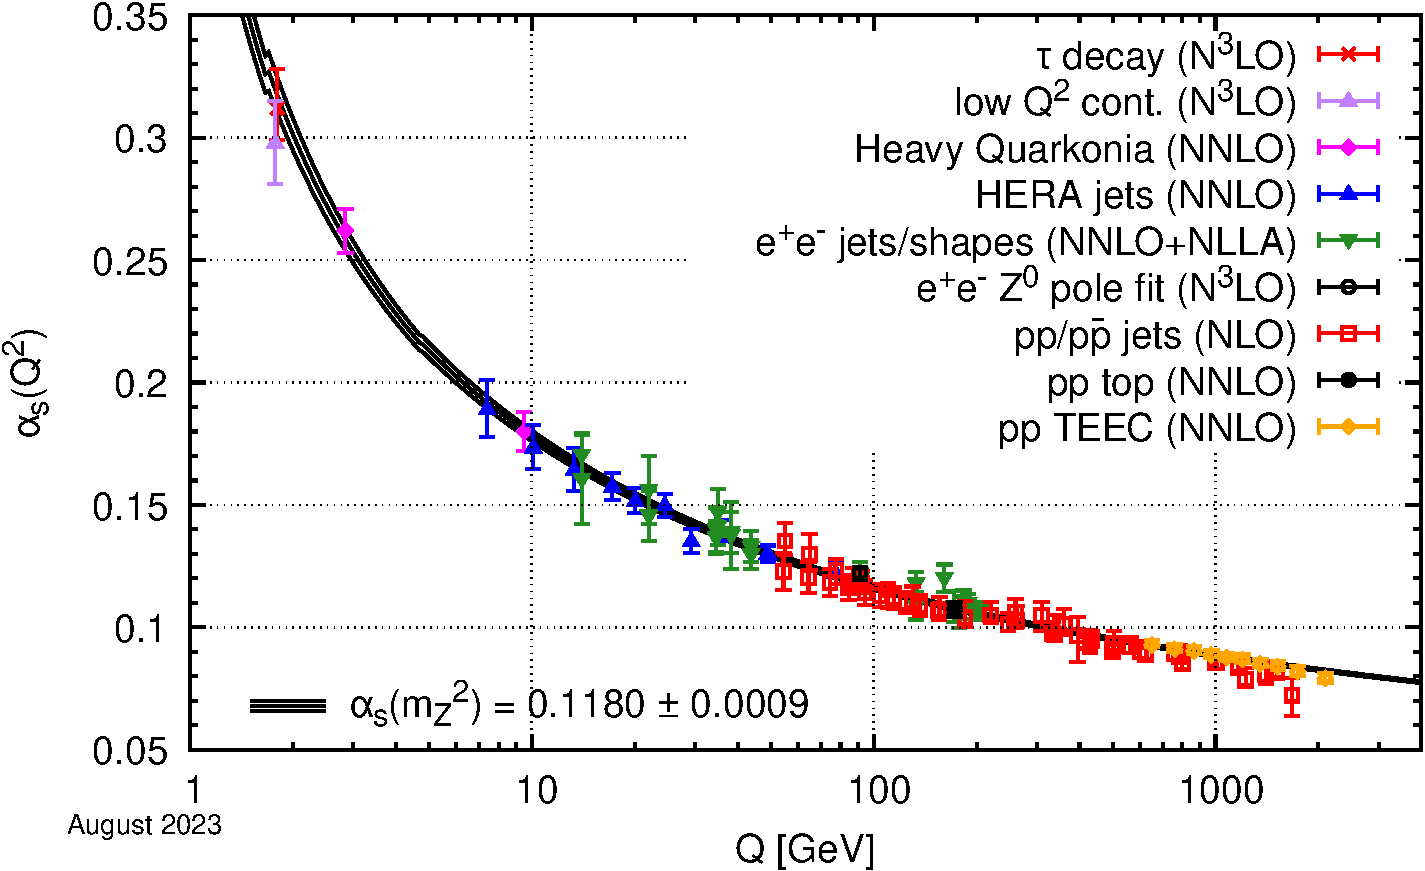
\includegraphics[width=0.6\linewidth]{2_theory/alphas}
    \caption{Medidas experimentales de la constante de acoplamiento de \ac{QCD} comparada con las predicciones calculadas a nivel de 5 loops~\cite{ParticleDataGroup2024}.}
    \label{fig:theory:sm:mathematical:qcd:alphas}
\end{figure}


\paragraph{Confinamiento y libertad asintótica}

Se dice que la constante de acoplamiento \textit{corre}, siendo grande a baja energía y haciéndose más pequeña a alta energía. De la \Eqn{\ref{eq:theory:sm:mathematical:qcd:alphas}}, a altas energías \(\alpha_s \to 0\) y en consecuencia, los quarks se comportan como partículas no acotadas, fenómeno conocido como libertad asintótica~\cite{Wilczek_Gross-1973,Politzer-1973}.
Por otro lado, para bajas energías (\(Q^2 \to 0\)), el acoplamiento \(\alpha_s\) aumenta divergentemente y por tanto \ac{QCD} da lugar al confinamiento de quarks y gluones~\cite{Glashow_Georgi-1974}. El confinamiento implica que ni los quarks ni los gluones pueden aparecer aislados sino que forman compuestos sin color llamados hadrones.
Además, a partir de la escala de corte infrarroja \(\Lambda_{\text{QCD}}\), donde la aproximación perturbativa a \(\alpha_s\) ya no es válida, la creación de pares quark-antiquark en el vacío es energéticamente más favorable que la separación de un par de quarks ligados. Por esta razón, a medida que pierden energía, los quarks y gluones producidos en un colisionador de protones sufren un proceso repetitivo conocido como hadronización, en el que se crean cascadas colimadas de hadrones, denominadas jets, que forman un cono desde el quark o gluón inicial.


\subsection{Interacciones hadrónicas en colisionadores protón-protón}
\label{subsec:theory:sm:hadron_interactions}

Como se discute en la \Sect{\ref{subsubsec:theory:sm:mathematical:qcd}}, la constante de acoplamiento \(\alpha_s\), que gobierna las interacciones fuertes entre quarks, tiene una fuerte dependencia de la escala de energía de cada interacción, modificando radicalmente la naturaleza de los procesos. La modelización de una colisión protón-protón en un experimento como lo es \ac{ATLAS}, en el que es necesario conocer su evolución desde la interacción entre los protones a \(\sqs \sim \tev\), hasta la interacción de las partículas en el estado final con los materiales activos y pasivos del detector a unos pocos GeV, representa un enorme reto ya que abarca regímenes de comportamiento \ac{QCD} muy diferentes. Dado que el \ac{LHC} es un colisionador de protones es importante disponer de una descripción muy precisa de la estructura de los protones, ya que una colisión \pp a muy altas energías consiste básicamente en colisionar los constituyentes de los mismos.

A energías muy altas, pero dentro del régimen perturbativo, la colisión entre dos protones puede estudiarse mediante el Modelo de Partones. Este modelo fue introducido por Feynman~\cite{Feynman-1969} y Bjorken~\cite{Bjorken-1969_1} a finales de los años 60 para interpretar la dispersión inelástica profunda electrón-núcleo en SLAC. Esta descripción ha demostrado ser una buena aproximación para interacciones partón-partón con gran transferencia de momento (es decir, el escalado de Bjorken~\cite{Bjorken-1969_2}), pero no es apropiada para modelizar la interacción a bajas energías.
Bajo esta abstracción, los partones incluyen no sólo los quarks de valencia (\(u\), \(\bar{u}\) y \(d\) en el caso del protón) sino también los pares de partículas y antipartículas en el mar de quarks y los gluones que median las interacciones entre ellos. El modelo asume una interacción permanente entre los partones, por lo que su momento individual es desconocido, aunque su fracción de momento con respecto al momento total del hadrón puede modelizarse como una variable aleatoria.
Además, en el caso de la verificación experimental, los quarks y gluones en el estado final no se observan directamente debido a la hadronización. En su lugar, se calcula una sección eficaz hadrónica efectiva, \(\sigma(\pp\to jj)\), entre los protones incidentes y los jets del estado final. Para realizar este paso, se utiliza el teorema de factorización~\cite{Ellis_Georgi_Politzer_Ross-1978,Feynman-1969,Collins_Soper_Sterman-book,Collins_Soper-1987}, que permite una separación sistemática entre las interacciones de corta distancia (de los partones) y las interacciones de larga distancia (responsables del confinamiento del color y de la formación de hadrones). Este teorema establece que la sección eficaz total para dos hadrones puede obtenerse ponderando y combinando las secciones eficaces para dos partones particulares. Esta ponderación se realiza utilizando lo que se conoce como una \ac{PDF1}, \(f_i(x,Q^2)\), que describe la densidad de partones para un partón de la especie \(i\) en un hadrón, con una fracción \(x\) de la energía-momento del hadrón cuando el hadrón se prueba a una escala de \(Q^2\). La sección eficaz para un proceso de dispersión dura \(\pp \to X\), iniciado por dos hadrones con cuadrimomentos \(P_1\) y \(P_2\) puede escribirse como:
\begin{equation}
    \label{eq:theory:sm:hadron_interactions:xs}
    \sigma_{\pp\to X} = \sum_{ij} \int_0^1 \dd{x_1} \dd{x_2} f_i(x_1, \mu_F^2) f_j(x_2, \mu_F^2) \, \hat{\sigma}_{ij}\left(p_1, p_2, \alpha_s(\mu_R^2), Q^2/\mu_R^2, Q^2/\mu_F^2 \right),
\end{equation}
donde \(x_1\) y \(x_2\) son las fracciones de momento transportadas por los partones interactuantes, y \(p_1 = x_1 P_1\) y \(p_2 = x_2 P_2\) son los momentos de los partones interactuantes. La sección eficaz partónica \(\hat{\sigma}_{ij}\), correspondiente a la interacción de los partones \(i\) y \(j\), se calcula a un orden fijo en \(\alpha_s\), que se evalúa a una cierta escala de renormalización \(\mu_R\) y escala de factorización \(\mu_F\). La escala de renormalización \(\mu_R\) es importante para absorber las divergencias \ac{UV} en los cálculos a órdenes superiores. La sección eficaz total se obtiene sumando todos los posibles sabores de partón e integrando todas las posibles fracciones de momento. Las \acp{PDF1}, \(f_i\) y \(f_j\), se evalúan a una escala de factorización, \(\mu_F\) , que puede considerarse como la escala que separa la física perturbativa de corta distancia de la física no perturbativa de larga distancia (es decir, separa los procesos duros de los blandos).

Si la expansión perturbativa se llevara a todos los órdenes, la sección eficaz en la \Eqn{\ref{eq:theory:sm:hadron_interactions:xs}} sería independiente de \(\mu_F\) y \(\mu_R\). Sin embargo, en el cálculo real de orden finito esto no es así. Suelen tomarse ambos como iguales, \(\mu_F = \mu_R = \mu\), elegidos a la escala típica \(Q^2\) del proceso, para minimizar la contribución de los términos de orden superior no calculados cuyas formas son logarítmicas \(\log\left(Q^2/\mu_R^2\right)\) y \(\log\left(Q^2/\mu_F^2\right)\). La dependencia de la predicción de \(\mu_R\) y \(\mu_F\) se asigna como incertidumbre teórica. El hecho de que la sección eficaz de un proceso deba ser independiente de la escala de factorización \(\mu_F\) condujo a las ecuaciones DGLAP (Dokshitzer-Gribov-Lipatov-Altarelli-Parisi)~\cite{Dokshitzer-1977,Gribov_Lipatov-1971,Altarelli_Parisi-1977}. Estas ecuaciones determinan la evolución de la \ac{PDF1} con \(Q^2\).
Para el caso del protón, la \Fig{\ref{fig:theory:sm:hadron_interactions:pdfs}} muestra las \acp{PDF1} evaluadas a dos escalas de factorización diferentes para todos los partones posibles.

\begin{figure}[ht!]
    \centering
    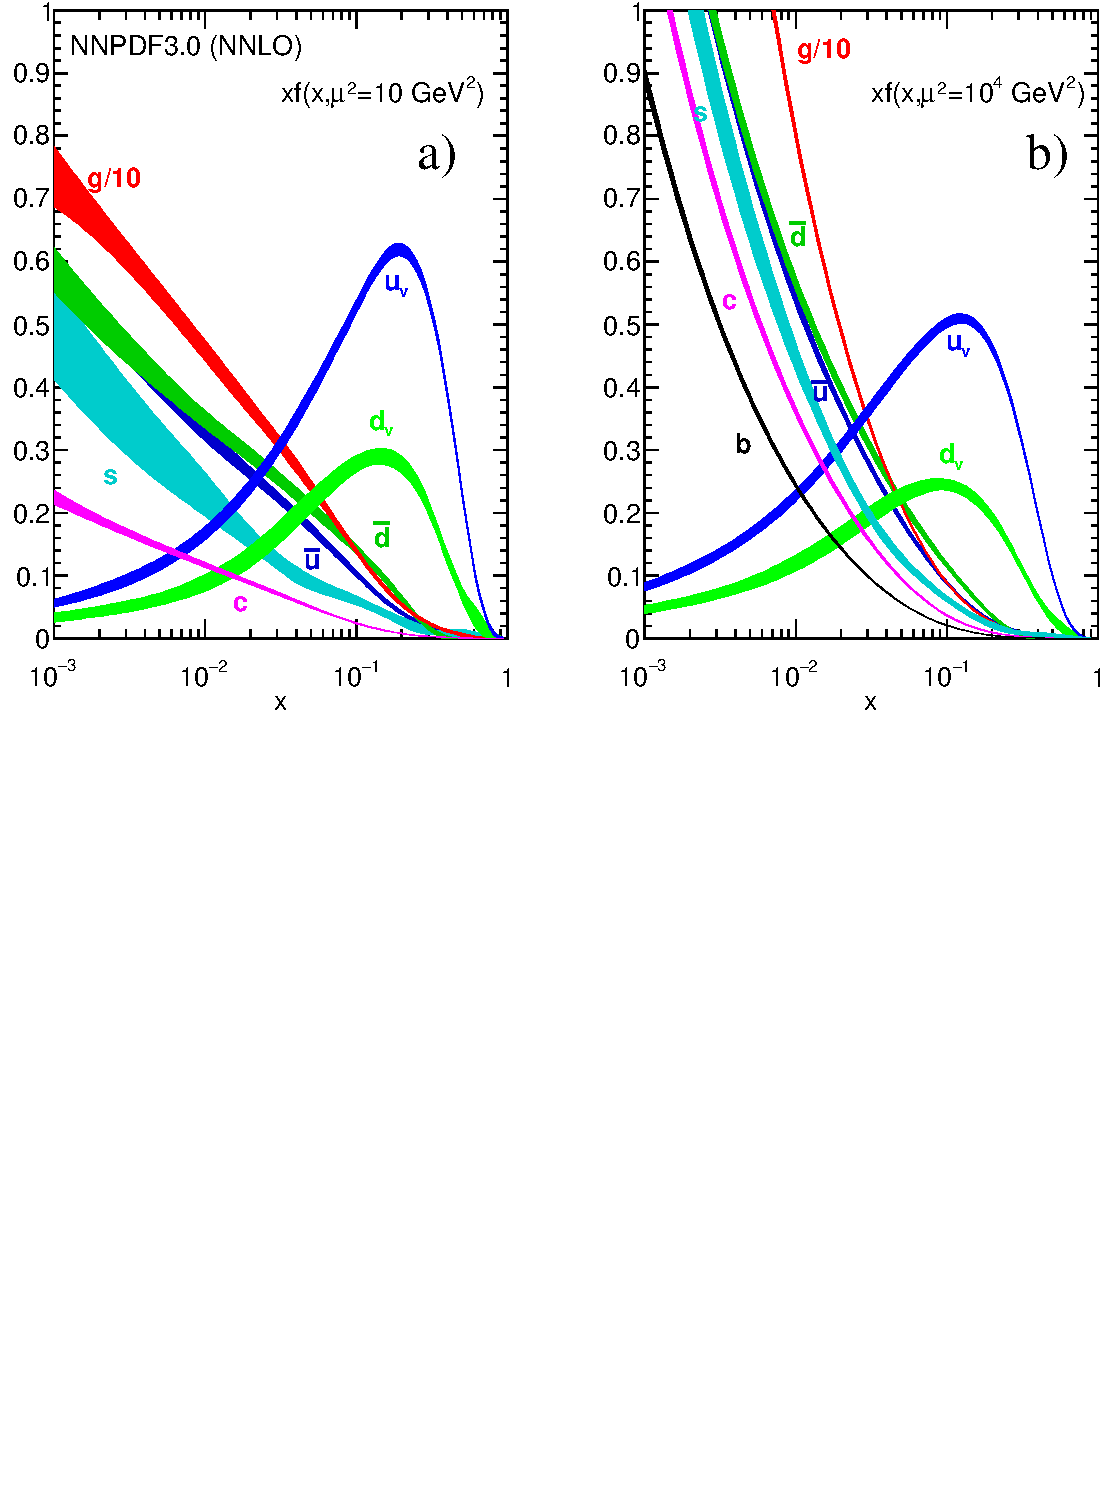
\includegraphics[width=0.7\linewidth]{2_theory/pdfs}
    \caption{Fracción del momento \(x\) del partón multiplicado por su correspondiente \acs{PDF1} \(f_i(x, Q^2)\) (donde \(i = u_v = u - \bar{u}, \, d_v = d - \bar{d},\, \bar{u},\, \bar{d},\, s\simeq\bar{s},\, c=\bar{c},\, b=\bar{b},\, g \)) obtenida por el análisis global a \ac{NNLO} NNPDF3.0~\cite{NNPDF} para dos escalas diferentes: \(\mu^2 = 10~\gev^2\) (izquierda) y \(\mu^2 = 10^4~\gev^2\) (derecha), utilizando \(\alpha_s(M_Z^2) = 0.118\). Las figuras son extraídas de la \Refn{\cite{ParticleDataGroup2020}}.}
    \label{fig:theory:sm:hadron_interactions:pdfs}
\end{figure}




\subsubsection{Descripción del proceso de colisión}

Inicialmente dos hadrones se acercan en un curso de colisión, donde cada hadrón puede pensarse como un grupo de partones esencialmente colineales caracterizados cuantitativamente por las \acp{PDF1}.
Se denomina como colisión dura a la colisión entre los dos partones procedentes uno de cada hadrón. Esta proceso puede ser calculado por una aproximación perturbativa hasta cierto orden en \(\alpha_s\).%, que corresponde al número de partones salientes.
En un escenario de colisión con partículas aceleradas que llevan carga \ac{EM} y cargas de color, procesos de bremsstrahlung pueden ocurrir antes y después de la colisión dura, como por ejemplo radiación de gluones como \(q \to qg\).
Las emisiones que se inician a partir de los dos protones que colisionan se denominan \ac{ISR}, mientras que las radiaciones de los partones salientes se denominan \ac{FSR}. Con el desarrollo de la lluvia de partones, la intensidad del campo de \ac{QCD} aumenta (véase la \Fig{\ref{fig:theory:sm:mathematical:qcd:alphas}}) a medida que los partones pierden energía y pueden romperse mediante la producción de pares quark-antiquark. Así, quarks y antiquarks pueden combinarse para producir un hadrón primario. La creación de hadrones como consecuencia del fenómeno de confinamiento se denomina \enquote{hadronización}. Los productos adicionales de la colisión que no están explícitamente relacionados con el proceso duro (radiación, restos de hadrones, productos de interacciones de múltiples partones, etc.), se suelen agrupar y denominar \ac{UE}. Una visualización de la colisión \pp se muestra en la \Fig{\ref{fig:theory:sm:hadron_interactions:parton_shower}}.



\begin{figure}[ht!]
    \centering
    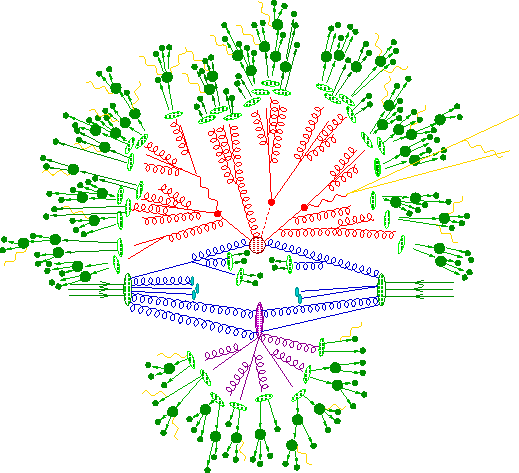
\includegraphics[width=0.7\linewidth]{2_theory/parton_shower}
    \caption{Ilustración de las etapas de una colisión hadrón-hadrón. El círculo rojo en el centro de la figura representa la colisión dura, rodeada por una estructura en forma de árbol que representa la radiación bremmstrahlung que simulan las \textit{parton showers}. El óvalo violeta en la parte inferior representa un ejemplo de un evento secundario de dispersión dura (\ac{UE}). El proceso de hadronización está representado por los óvalos verdes claro, mientras que los círculos verdes oscuro indican los decaimientos hadrónicos. Finalmente, las líneas amarillas señalan la radiación de fotones.~\cite{Hoche-2015}.}
    \label{fig:theory:sm:hadron_interactions:parton_shower}
\end{figure}



A lo largo de los años, diferentes experimentos del \ac{LHC} han medido secciones eficaces de diferentes procesos del \ac{SM}. La \Fig{\ref{fig:theory:sm:hadron_interactions:sm_results}} muestra la buena concordancia entre las secciones eficaces medidas por \ac{ATLAS} de algunos procesos y sus predicciones teóricas.


\begin{figure}[ht!]
    \centering
    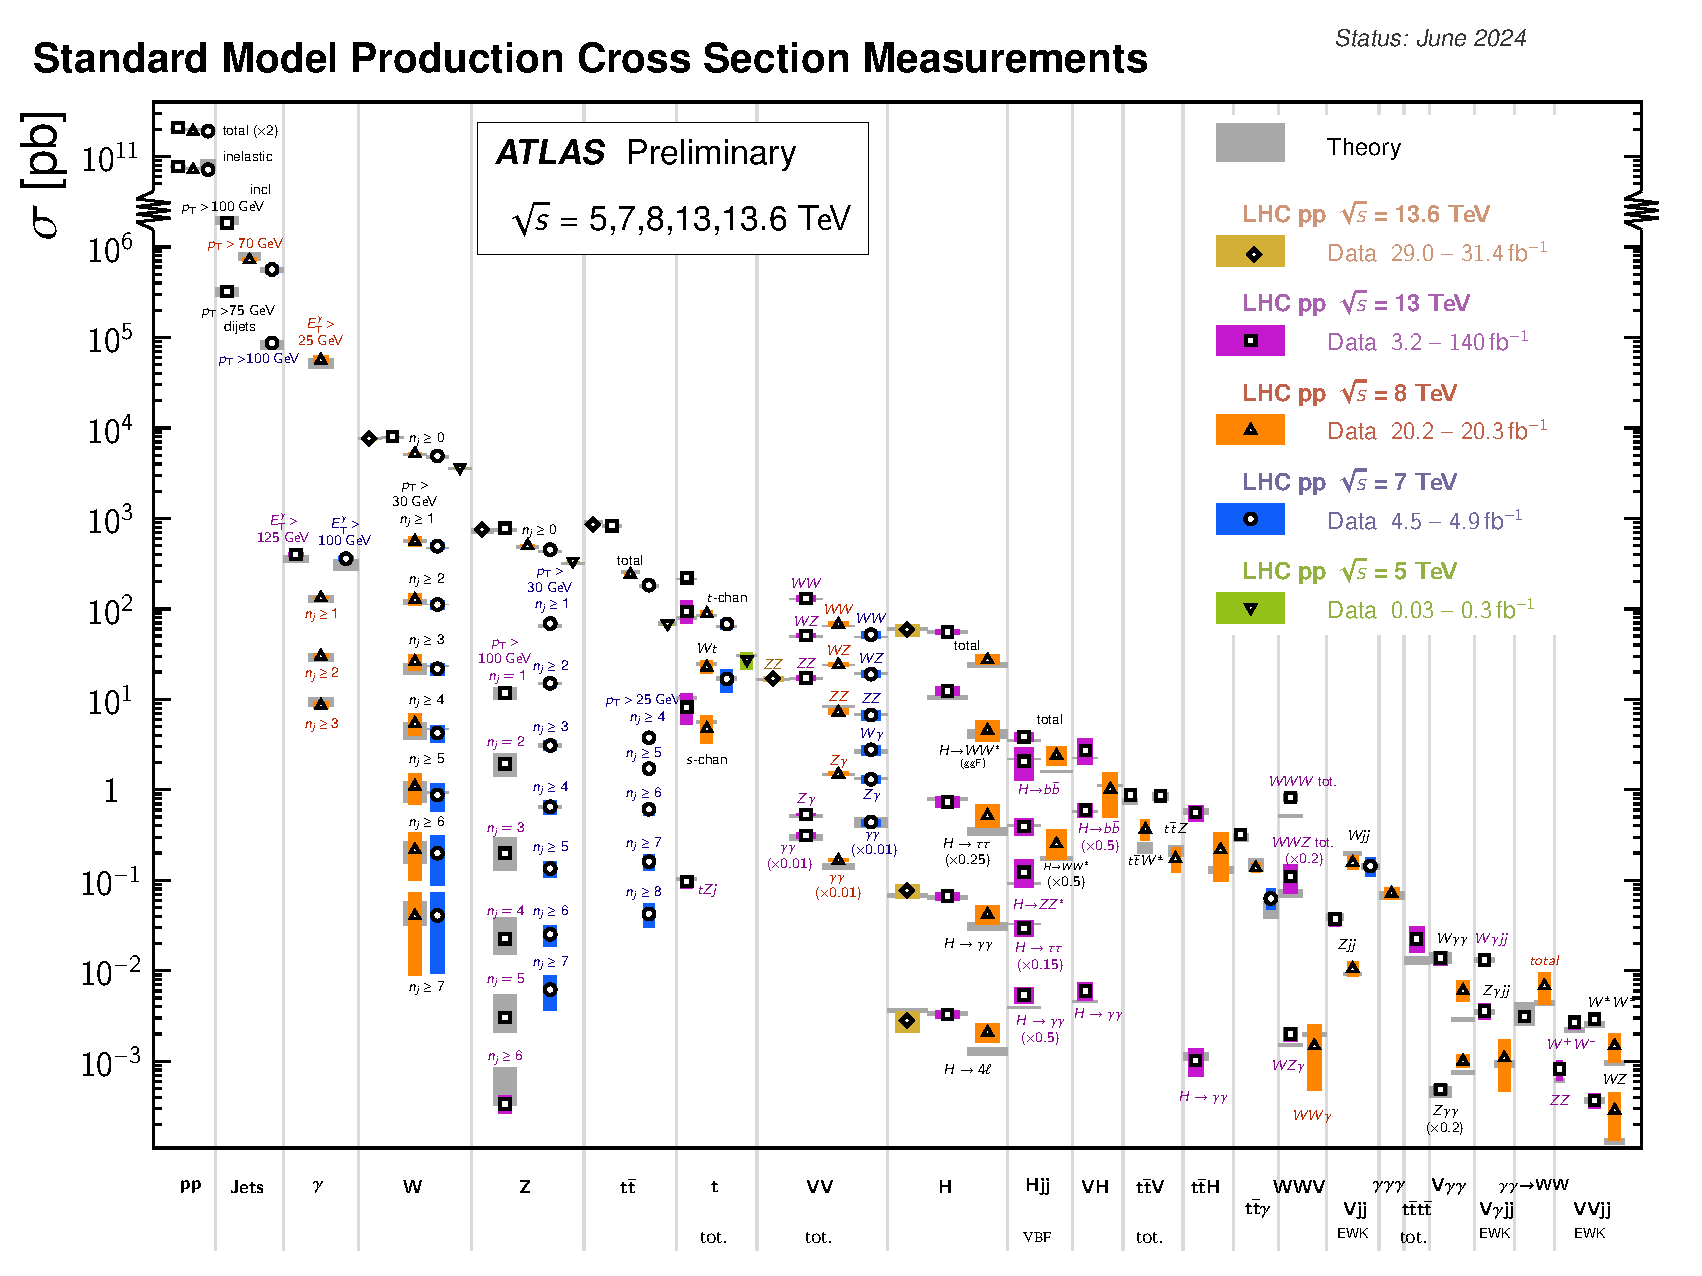
\includegraphics[width=0.8\linewidth]{2_theory/sm_measurements}
    \caption{Resumen de diversas medidas experimentales de las secciones eficaces de producción de diferentes procesos del \ac{SM}, comparadas con las predicciones teóricas~\cite{ATLAS-SM_Measurements}.}
    \label{fig:theory:sm:hadron_interactions:sm_results}
\end{figure}



\subsection{Teoría de producción de fotones \textit{prompt}}
\label{subsec:theory:sm:prompt_photon}


Los fotones de alto momento transverso originados en la colisión \pp (\enquote{prompt}) permiten investigar una gran variedad de procesos en escenarios de colisiones \pp, ya sea para realizar medidas de precisión del \ac{SM} o para llevar a cabo búsqueda de nueva física (\ac{BSM}). Una de las grandes ventajas de estos procesos es que las señales dejadas en los detectores por los fotones son mucho más limpias que las dejadas por jets, en donde además se cuenta con menores incertezas sistemáticas de reconstrucción e identificación.

% la interacción dura y su producción en colisiones protón-protón, \(\pp \to \gamma+X\), ofrece ciertas ventajas sobre otros análisis en eventos de producción de jets, el proceso más abundante en los colisionadores hadrónicos, proporcionando un escenario ideal para investigaciones sobre la teoría \ac{QCD}. En este caso, la presencia de un vértice \ac{QED} a \ac{LO} hace que los cálculos teóricos sean más confiables y da acceso a un rango más bajo de \pt. Además, la resolución energética de los calorímetros electromagnéticos es en general mejor que la de los calorímetros hadrónicos\footnote{Una descripción de ambos calorímetros se brinda en el \Ch{\ref{ch:atlas}}.}, y las incertidumbres sistemáticas en la escala de energía de los fotones son menores. Debido al hecho de que los fotones no hadronizan (véase \Sect{\ref{subsec:theory:mc_simulation:hadronisation}}), la dirección y la energía de los fotones se miden directamente en el calorímetro sin necesidad de contar con la reconstrucción de un jet.

La producción de fotones prompt tiene lugar a través de dos procesos: el proceso de fotones directos (D) en el que el fotón surge directamente de la interacción dura, y el proceso de fotones de fragmentación (F), en el que el fotón se emite en la fragmentación de un partón de alto momento transverso~\cite{Szczurek_Pietrycki-2007,Belghobsi_Fontannaz-2009}. Desde un punto de vista topológico, cuando se produce un fotón directo, generalmente está separado de la actividad hadrónica, mientras que un fotón producido a partir de un proceso de fragmentación, lo más probable es que esté acompañado de hadrones.

A \ac{LO} en teoría de perturbaciones, hay dos subprocesos que contribuyen a la producción de fotones directos: (a) el proceso Compton \(qg \to \gamma q\) y (b) el proceso de aniquilación \(\qqbar \to \gamma+g\), mostrados en las \Figs{\ref{fig:theory:sm:prompt_photon:feynman_lo_direct:compton}}{\ref{fig:theory:sm:prompt_photon:feynman_lo_direct:annihilation}}, respectivamente. A mediano y gran \(x\) (fracción de momento del partón) hay una jerarquía natural de distribuciones de partones en el protón, \(q \gg g \gg \bar{q}\), mientras que a pequeño \(x\), \(g \gg q,\bar{q}\) (\Fig{\ref{fig:theory:sm:hadron_interactions:pdfs}}). Como consecuencia, en las colisiones protón-protón, el proceso Compton \(qg\) domina esencialmente en todo el rango \pt. Esto hace que la producción prompt de fotones sea particularmente útil para restringir la distribución de gluones.

\begin{figure}[ht!]
    \centering
    \begin{subfigure}[h]{0.49\linewidth}
        \centering
        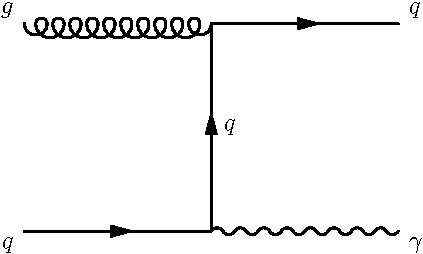
\includegraphics[width=0.7\linewidth]{2_theory/diagrams/gammajet_compton}
        \caption{Compton.}
        \label{fig:theory:sm:prompt_photon:feynman_lo_direct:compton}
    \end{subfigure}
    \hfill
    \begin{subfigure}[h]{0.49\linewidth}
        \centering
        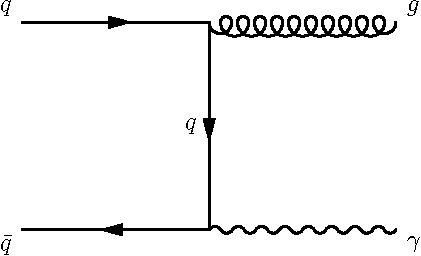
\includegraphics[width=0.7\linewidth]{2_theory/diagrams/gammajet_annihilation}
        \caption{Aniquilación.}
        \label{fig:theory:sm:prompt_photon:feynman_lo_direct:annihilation}
    \end{subfigure}
    \caption{Diagramas de Feynman de producción de fotones directos a \ac{LO} en colisiones \pp.}
    \label{fig:theory:sm:prompt_photon:feynman_lo_direct}
\end{figure}

Las correcciones a \ac{NLO} de este proceso se presentan en la \Fig{\ref{fig:theory:sm:prompt_photon:feynman_nlo_direct}}. En la \Fig{\ref{fig:theory:sm:prompt_photon:feynman_nlo_direct:gluon}}, existe una singularidad colineal cuando los momentos del quark y el gluón del estado final son paralelos. Esta divergencia se cancela cuando se suman las contribuciones real y virtual del gluón (un ejemplo de una contribución virtual se muestra en la \Fig{\ref{fig:theory:sm:prompt_photon:feynman_nlo_direct:gluon_virtual}}) y el efecto neto es una corrección finita \(\mathcal{O}(\alpha_s)\) al proceso \ac{LO}.

\begin{figure}[ht!]
    \centering
    \begin{subfigure}[h]{0.49\linewidth}
        \centering
        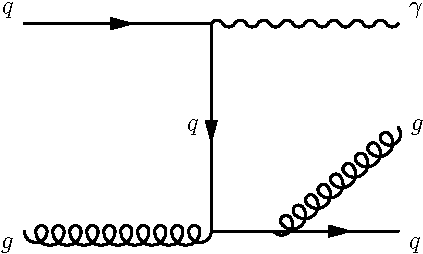
\includegraphics[width=0.7\linewidth]{2_theory/diagrams/gammajet_fsr_gluon}
        \caption{\Ac{FSR} de gluón.}
        \label{fig:theory:sm:prompt_photon:feynman_nlo_direct:gluon}
    \end{subfigure}
    \hfill
    \begin{subfigure}[h]{0.49\linewidth}
        \centering
        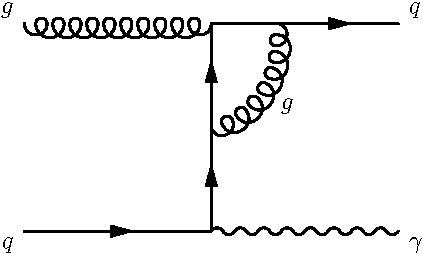
\includegraphics[width=0.7\linewidth]{2_theory/diagrams/gammajet_nlo_direct_virtualcorrection}
        \caption{Correcciones virtuales de gluones.}
        \label{fig:theory:sm:prompt_photon:feynman_nlo_direct:gluon_virtual}
    \end{subfigure}\\
    \caption{Diagramas de Feynman de producción de fotones directos a \ac{NLO} en colisiones \pp.}
    \label{fig:theory:sm:prompt_photon:feynman_nlo_direct}
\end{figure}

Asimismo, en la \Fig{\ref{fig:theory:sm:prompt_photon:feynman_nlo_frag}} se muestran las correcciones a la producción de fotones de fragmentación a \ac{NLO}. Al igual que para el caso de fotones directos, en los diagramas de las \Figs{\ref{fig:theory:sm:prompt_photon:feynman_nlo_frag:photon_fsr}}{\ref{fig:theory:sm:prompt_photon:feynman_nlo_frag:photon_isr}} se observan singularidades colineales pero, esta vez, cuando los momentos del fotón y del quark son paralelos. Esta singularidad, sin embargo, no se cancela sino que tiene que ser absorbida en una función de fragmentación de fotones \(D_q^{\gamma} (z, \mu^2_f )\) que representa la probabilidad de encontrar un fotón portando fracción de momento longitudinal \(z\) en un jet de quarks a escala \(\mu_f\). Estas correcciones a \ac{NLO} de la componente de fragmentación contiene también todos los procesos en los que un partón del estado final fragmenta para producir un fotón (dentro de la cascada partónica), incluido aquel donde el fotón es colineal al al momento del partón originario (\Figs{\ref{fig:theory:sm:prompt_photon:feynman_nlo_frag:quark}}{\ref{fig:theory:sm:prompt_photon:feynman_nlo_frag:gluon}}). Esta función de fragmentación no es calculable en teoría de perturbaciones y obedece a una ecuación de evolución DGLAP similar a la de las funciones de fragmentación hadrónicas. La contribución a la sección eficaz de la \Fig{\ref{fig:theory:sm:prompt_photon:feynman_nlo_frag}} contiene un factor de la forma
\begin{equation}
    \label{eq:theory:sm:prompt_photon:fragmentation_contribution}
    \hat{\sigma}(qg \to qg) \oplus D_q^{\gamma} \left(z, \mu_f^2\right).
\end{equation}
La función de fragmentación de fotones aumenta uniformemente con la escala en todo el rango de \(z\), es decir, \(D_k^{\gamma} \left(z, \mu_f^2\right) \sim d^{\gamma}(z)\ln(\mu^2)\) cuando \(\mu^2 \to \infty\). Cuando \(\pt \gtrsim \gev\), el crecimiento en la forma de \(\ln \pt^2\) de la función de fragmentación en la \Eqn{\ref{eq:theory:sm:prompt_photon:fragmentation_contribution}} compensa uno de los acoplamientos \(\alpha_s \left(\pt^2\right)\) en la sección eficaz del subproceso y la contribución es efectivamente de orden \(\alpha_s \left(\pt^2\right) \alpha_{EM}\), es decir, la misma que la contribución a \ac{LO}.


\begin{figure}[ht!]
    \centering
    \begin{subfigure}[h]{0.49\linewidth}
        \centering
        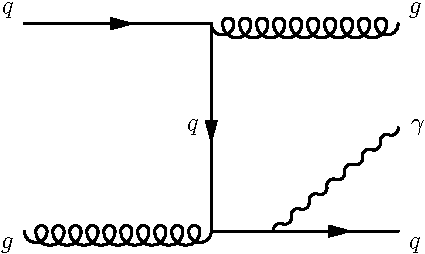
\includegraphics[width=0.7\linewidth]{2_theory/diagrams/gammajet_fsr}
        \caption{\Ac{FSR} de fotón.}
        \label{fig:theory:sm:prompt_photon:feynman_nlo_frag:photon_fsr}
    \end{subfigure}
    \hfill
    \begin{subfigure}[h]{0.49\linewidth}
        \centering
        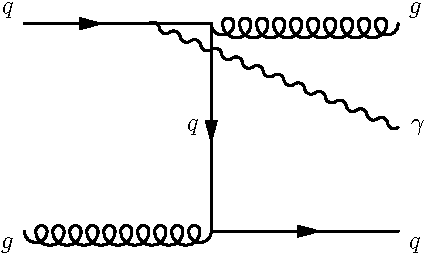
\includegraphics[width=0.7\linewidth]{2_theory/diagrams/gammajet_isr}
        \caption{\Ac{ISR} de fotón.}
        \label{fig:theory:sm:prompt_photon:feynman_nlo_frag:photon_isr}
    \end{subfigure}\\
    \begin{subfigure}[h]{0.49\linewidth}
        \centering
        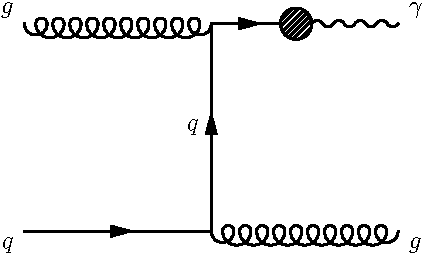
\includegraphics[width=0.7\linewidth]{2_theory/diagrams/gammajet_fragmentation_quark}
        \caption{Fragmentación de un fotón de un quark a \ac{NLO}.}
        \label{fig:theory:sm:prompt_photon:feynman_nlo_frag:quark}
    \end{subfigure}
    \hfill
    \begin{subfigure}[h]{0.49\linewidth}
        \centering
        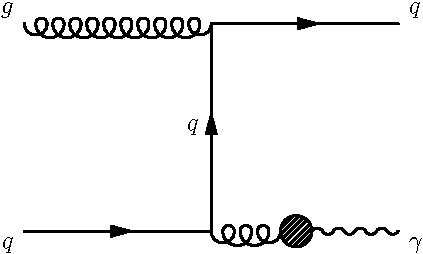
\includegraphics[width=0.7\linewidth]{2_theory/diagrams/gammajet_fragmentation_gluon}
        \caption{Fragmentación de un fotón de un gluón a \ac{NLO}.}
        \label{fig:theory:sm:prompt_photon:feynman_nlo_frag:gluon}
    \end{subfigure}\\
    \caption{Diagramas de Feynman de producción de fotones de fragmentación a \ac{NLO} en colisiones \pp.}
    \label{fig:theory:sm:prompt_photon:feynman_nlo_frag}
\end{figure}






La sección eficaz diferencial inclusiva en \(\etgam\) para la producción de un fotón no aislado viene dada por la suma de las contribuciones directas y de fragmentación:
\begin{align}
    \dv{\sigma}{\etgam} &= \dv{\sigma_{\text{dir}}}{\etgam} + \dv{\sigma_{\text{frag}}}{\etgam} \nonumber\\
    &= \sum_{a,b=q,\bar{q},g} \int \dd{x_a} \dd{x_b} f_a\left(x_a, \mu_F^2\right) f_b\left(x_b, \mu_F^2\right) \times \nonumber\\
    &\quad\quad
    \Biggl[
        \dd{\hat{\sigma}^{\gamma}_{ab} \left(p^{\gamma}; x_a, x_b, \mu_R, \mu_F, \mu_f\right)}
        + \nonumber\\
    &\quad\quad\quad\quad
    \sum_{c=q,\bar{q}, g} \int_{z_{\min}}^{1} \frac{\dd{z}}{z^2} \dd{\hat{\sigma}^c_{ab} \left(p^{\gamma}; x_a, x_b, z, \mu_R, \mu_F, \mu_f\right)} D_c^{\gamma} \left(z, \mu_f^2\right)
    \Biggr],
\end{align}
donde \(D_c^{\gamma} \left(z,\mu_f^2\right)\) es la función de fragmentación de un partón \(c\) a un fotón que lleva la fracción de momento \(z\), \(f_a \left(x_a, \mu^2_F \right)\) es la \ac{PDF1} de un partón \(a\), \(\mu_R\) y \(\mu_F\) son las escalas estándar de renormalización y factorización y \(\mu_f\) es la escala de fragmentación. Las correcciones de la componente directa de la sección eficaz partónica \(\hat{\sigma}^{\gamma}_{ab}\) se conocen hasta el \ac{NNLO} en \ac{pQCD}, mientras que la componente de fragmentación \(\hat{\sigma}^c_{ab}\) sólo se conoce a \ac{NLO}.

A \ac{LO}, los cálculos teóricos para los procesos directos y de fragmentación convergen por separado y pueden considerarse independientemente. Sin embargo, esta distinción no tiene significado físico más allá de \ac{LO}, ya que ambos tipos de procesos deben considerarse al mismo tiempo para cancelar las singularidades colineales e infrarrojas del estado final. Por lo tanto, más allá del \ac{LO}, tanto los procesos directos como los de fragmentación no pueden considerarse por separado. Desde un punto de vista teórico, la distinción viene definida por una elección arbitraria. Se deriva de la necesidad de factorizar las singularidades colineales del estado final y absorberlas en las funciones de fragmentación. Esta factorización requiere la introducción de una escala de fragmentación arbitraria \(\mu_f\), que es un parámetro no físico. En términos más generales, depende de la elección arbitraria del esquema de factorización, que define la parte finita de las correcciones de orden superior que se absorbe en las funciones de fragmentación junto con las singularidades; la parte finita restante se incluye entonces en las contribuciones de orden superior a las secciones eficaces partónicas. La dependencia de esta arbitrariedad y, en particular, de \(\mu_f\) se cancela sólo en la suma de las contribuciones directas y de fragmentación, por lo que sólo esta suma es un observable físico.






\section{Física Más allá del Modelo Estándar}
\label{sec:theory:bsm}

En la sección anterior se han descripto brevemente el \ac{SM}, junto con resultados de \ac{ATLAS} que muestran un muy buen acuerdo del \ac{SM} con los datos experimentales. A pesar de ser una de las teorías más exitosas de la física en general, el modelo tiene naturalmente un rango de validez.
Sin embargo, no puede considerarse la teoría definitiva ya que tiene ciertas limitaciones tanto desde el punto de vista teórico como experimental. El \ac{SM} se sigue considerando una teoría efectiva, una aproximación a baja energía de una teoría más fundamental. Hay tres tipos populares de teorías de la nueva física: (i) modelos con una simetría extendida o sector escalar, (ii) teoría de mayores dimensiones y (iii) fermiones compuestos (es decir, los fermiones del \ac{SM} ya no son elementales~\cite{Kuhn_Zherwas-1984,Cabibbo_Maiani_Srivastava-1984,DeRújula_Maiani_Petronzio-1984,Baur_Spira_Zerwas-1990,Bhattacharya_Chauhan_Choudhary_Choudhury-2009,Zhan_Li_Liu_Li-2016}).
A continuación, se presenta una vista general de las principales deficiencias del \ac{SM}. Luego, se discuten los modelos teóricos utilizados en la búsqueda llevada a cabo en esta tesis, que permiten resolver algunas de las cuestiones que el \ac{SM} no puede responder.

\begin{itemize}
    \item \underline{Gravedad:} Una de las principales limitaciones del \ac{SM} es la imposibilidad de incluir la gravedad del mismo modo que otras interacciones. No sólo incluir la gravedad en la teoría no es suficiente para explicar las observaciones, sino que las teorías matemáticas utilizadas en el \ac{SM} son prácticamente incompatibles con la formulación de la Relatividad General.
    \item \underline{Problema de jerarquías:} En el contexto de la física de altas energías se produce un problema de jerarquía cuando el valor fundamental de algún parámetro físico (como una constante de acoplamiento o una masa) en algún Lagrangiano es enormemente diferente de su valor efectivo, que es el valor que se mide en un experimento. Normalmente, el valor renormalizado de los parámetros se aproxima a sus valores fundamentales y, en general, los problemas de jerarquía están relacionados con el ajuste fino de los parámetros en la teoría. En física de partículas el problema de jerarquías es la diferencia entre la escala \ac{EW} \(M_W \sim 10^2~\gev\) y la escala de Planck, donde los efectos de la gravedad son relevantes \(M_P\sim10^{19}~\gev\), cuya relación es \(M_W / M_P \sim 10^{-17}\).
    \item \underline{\acf{DM}:} Una pista hacia la incompletitud del \ac{SM} es la presencia de \ac{DM}. Según mediciones astrofísicas y consideraciones cosmológicas~\cite{Zwicky-1937,Rubin_Kent-1970,Planck-2014,Clowe-2006,Brada-2008}, la materia conocida sólo representa menos del \(5\%\) del total del universo. Por otra parte, el \(23\%\) del total de la materia está asociado a un tipo de materia desconocida, denominada \ac{DM}, ya que no absorbe radiación \ac{EM}, pero es masiva al tener efectos gravitatorios considerables sobre la materia visible. La única partícula del \ac{SM} que podría ser un candidato \ac{DM} viable es el neutrino, pero como su masa es demasiado pequeña para explicar estos fenómenos, se ha descartado.
    \item \underline{Masa de los neutrinos:} La observación de la oscilación de los neutrinos implica que, aunque ellos tienen una masa muy pequeña, ésta no es nula, en contraste con la predicción del \ac{SM}. Aunque existen varios mecanismos para incluirlos en el \ac{SM}, no hay pruebas suficientes para saber cuál es la forma correcta y algunos modelos proponen la existencia de nuevas partículas pesadas aún no observadas~\cite{GellMann_Ramond_Slansky-2010,Glashow-1980,Ramond-2005}.
    \item \underline{Tres familias de fermiones:} El hecho de que sólo se hayan observado tres familias de fermiones también es uno de los gran interrogantes del \ac{SM} ya que no tiene ninguna explicación teórica. Como ya se ha mencionado, estas familias de quarks y leptones sólo difieren en la masa, mientras que todos los números cuánticos permanecen idénticos. Además, otro interrogante es por qué existen dos familias extras a las de la materia estable del Universo.
\end{itemize}





\subsection{Teorías de quarks compuestos}
\label{subsec:theory:bsm:qstar}

En las teorías de fermiones compuestos, éstos ya no son los constituyentes fundamentales de la materia sino estados ligados de partículas denominadas \textit{preones}~\cite{Pfeil-1981}. Se postula que estas últimas experimentan una fuerza desconocida hasta ahora a causa de una interacción de gauge asintóticamente libre pero confinante~\cite{Hooft-1980}, que se hace muy fuerte a una escala característica \(\Lambda\), dando lugar así a los fermiones compuestos. En muchos de estos modelos~\cite{Pati_Salam_Strathdee-1975,Fritzsch_Mandelbaum-1981,Baur_Fritzsch-1984}, aunque no en todos, los quarks y los leptones comparten al menos algunos constituyentes comunes. Tal hipótesis conduce naturalmente a la existencia de estados excitados de fermiones a una escala de masa comparable a la dinámica de la nueva interacción. Además, estos modelos brindan una solución al problema de las 3 generaciones de fermiones del \ac{SM}, dado que estas generaciones serían diferentes configuraciones o estados excitados de los preones.

Como los \enquote{estados excitados} sí sufren las interacciones de gauge del \ac{SM}, pueden producirse en colisionadores que operen a energías suficientemente altas. Al producirse, decaerían en partículas del \ac{SM} siendo un canal particularmente favorable el decaimiento radiativo en un fermión y un bosón gauge (fotón, \Wboson, \Zboson, o gluón). Si los quarks y los leptones no son constituyentes fundamentales sino que son compuestos, este hecho podría, en principio, revelarse mediante un exceso de datos a escalas de energía comparables a la escala de composición \(\Lambda\) en las colisiones \pp en el \ac{LHC}. Si el valor de \(\Lambda\) no es demasiado alto, entonces se pueden producir \ac{EQ} \textit{on-shell}, mientras que a energías muy por debajo de \(\Lambda\), tales excitaciones podrían manifestarse a través interacciones de contacto de cuatro fermiones que involucrara sólo partículas del \ac{SM}.

En general, las interacciones entre los \acp{EQ} (\qstar) y los bosones gauge pueden escribirse como~\cite{Zhan_Li_Liu_Li-2016}:
\begin{equation}
    \mathcal{L}_{\text{gauge}} = 
    \frac{1}{2\Lambda}
    \overline{\qstar_R}
    \sigma^{\mu\nu}
    \left[
        g_s f_s \frac{\lambda_a}{2} G_{\mu\nu}^a +
        g f \frac{\tau}{2} W_{\mu\nu} +
        g' f' \frac{Y}{2} B_{\mu\nu} +
    \right]
    q_L
    + \text{H.c},
\end{equation}
donde \(G_{\mu\nu}^a\), \(W_{\mu\nu}\) y \(B_{\mu\nu}\) son los tensores de intensidad de campo de los campos gauge SU(3), SU(2) y U(1), respectivamente. Los coeficientes \(g_s\), \(g = e / \sin \theta\), \(g' = e / \cos \theta\) son los acoplamientos gauge fuerte y \ac{EW}, \(\lambda_a\) es la matriz de Gell-Mann, \(\tau\) es la matriz de Pauli y la hipercarga débil es \(Y = 1/3\), respectivamente. \(\Lambda\) es la escala de composición y \(f_s, \, f, \, f'\) son parámetros determinados por la dinámica de composición que representan la intensidad de las interacciones entre el \acp{EQ} y los campos del \ac{SM}. Los diagramas de Feynman de los canales \(s\) y \(t\), a \ac{LO}, para dicho proceso se presentan en la \Fig{\ref{fig:theory:bsm:diagrams}}. Finalmente, la amplitud del decaimiento de \acp{EQ} a un fotón y un quark puede calcularse a \ac{LO}~\cite{Zhan_Li_Liu_Li-2016} como:
\begin{equation}
    \Gamma\left(\qstar \to q \gamma\right) =
    \frac{1}{4}
    \alpha
    \left(f \tau_3 + f' \frac{Y}{2}\right)^2
    \frac{\mq^3}{\Lambda^2}.
\end{equation}
que aumenta con la masa \mq del \ac{EQ} si se considera \(\Lambda = \mq\).


\begin{figure}[ht!]
    \centering
    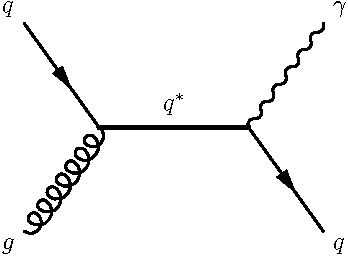
\includegraphics[width=0.3\linewidth]{2_theory/diagrams/qstar_gammajet_s_channel}
    \hspace{1cm}
    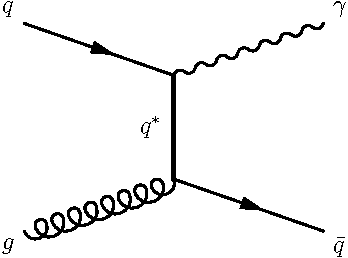
\includegraphics[width=0.3\linewidth]{2_theory/diagrams/qstar_gammajet_t_channel}
    \caption{Diagramas de Feynman de la producción de \ac{EQ} en colisiones \pp y su decaimiento en un quark y photon en el canal \(s\) (izquierda) y \(t\) (derecha).}
    \label{fig:theory:bsm:diagrams}
\end{figure}


En el \ac{SM} no hay un proceso de producción de una resonancia que decaiga en un par fotón+jet producido en colisiones \pp y la producción directa de fotón+jet a \ac{LO} ocurre vía dispersión Compton o aniquilación \qqbar, como se describió en la \Sect{\ref{subsec:theory:sm:prompt_photon}}. Como resultado, la distribución de la masa invariante \gammajet (\myj) cae rápidamente. De esta forma, un \ac{EQ} pesado que decae en un par \gammajet puede ser descubierto si existe. En lo que sigue de la tesis, de los modelos de \ac{EQ} que se estudian, sólo se considerarán los que decaen en un fotón y un jet. En el \Ch{\ref{ch:samples}} se da información sobre las secciones eficaces y las formas de las señales en el detector \ac{ATLAS}.

\subsection{Teorías con dimensiones extras}
\label{subsec:theory:bsm:qbh}

Explicar el problema de jerarquía, el enorme gap entre la escala \ac{EW} y la escala de Planck, ha sido una de las principales motivaciones para construir extensiones del \ac{SM}, como los modelos con supersimetría tecnicolor o de baja energía. Es notable que estas grandes estructuras teóricas, como lo son el \ac{SM} y la Teoría de Relatividad General, se hayan construido sobre el supuesto de la existencia de dos escalas de energía fundamentales muy dispares. Sin embargo, existe una diferencia importante entre estas escalas. Mientras que las interacciones \acp{EW} se han investigado a distancias cercanas a \(\sim m_W^{-1}\), las fuerzas gravitatorias no se han investigado ni remotamente a distancias \(\sim m_P^{-1}\).

Las propuestas de un espacio-tiempo con más de tres dimensiones espaciales se remontan a los años 20, principalmente a través de los trabajos de Kaluza y Klein, en un intento de unificar las fuerzas de la naturaleza~\cite{Bailin_Love-1987}. Aunque su idea inicial fracasó, el formalismo que ellos y otros desarrollaron sigue siendo útil hoy en día. Hacia 1980, la teoría de cuerdas propuso de nuevo ampliar el número de dimensiones espaciales, esta vez como requisito para describir una teoría coherente de la gravedad cuántica. Se suponía que las dimensiones extra se compactarían a una escala cercana a la de Planck por lo que no serían comprobables experimentalmente en un futuro próximo.

Arkani-Hamed, Dimopoulos y Dvali (ADD)~\cite{ADD-1998} dieron un enfoque diferente demostrando que la debilidad de la gravedad podría explicarse postulando dos o más dimensiones extra planas en las que sólo podría propagarse la gravedad. El tamaño de estas dimensiones extra debería oscilar entre aproximadamente un milímetro y \(\sim 1/\tev\), lo que daría lugar a posibles consecuencias observables en experimentos actuales y futuros. Otro enfoque, de Randall y Sundrum (RS)~\cite{RS1-1999_1,RS1-1999_2}, postula un espacio-tiempo Anti-deSitter (AdS) de cinco dimensiones con geometría deformada, donde la compactificación es de la escala de \(1/\tev\).

Estos modelos de gravedad de baja escala~\cite{Antoniadis_Arkani_Dimopoulos_Dvali-1998,ADD-1998,RS1-1999_1,RS1-1999_2,Dvali-2008,Dvali-2010} permiten la producción de \ac{QBH} en colisiones de partículas~\cite{Argyres-1998,Banks-1999,Giddings-2002}.
Los \ac{QBH}, a diferencia de los semiclásicos, muestran diferencias significativas a medida que su masa se aproxima a la escala de Planck. Los agujeros negros semiclásicos decaen térmicamente perdiendo masa a la temperatura de Hawking con un efecto mínimo en el espacio-tiempo circundante. Sin embargo, a medida que la masa del agujero negro disminuye y se acerca a la escala de Planck, la influencia de la reacción de retroceso en el espacio-tiempo se vuelve sustancial y el agujero negro ya no puede mantener el equilibrio térmico con su radiación. Cuando la longitud de onda Compton del agujero negro supera su radio de Schwarzschild, comienza a aparecer un comportamiento cuántico que podría conferirle propiedades similares a las de las partículas. En este punto, los conceptos de temperatura y entropía bien definidos ya no son válidos, lo que hace improbable que estos agujeros negros decaigan térmicamente~\cite{Meade-2008,Alberghi-2006,Alberghi-2007}.

Centrándose en agujeros negros con una masa ligeramente superior a la escala de Planck, se espera que los decaimientos de los \ac{QBH} no sigan un patrón térmico. En su lugar, es probable que dominen los decaimientos en unas pocas partículas y que estos procesos tengan lugar en una pequeña región del espacio-tiempo. Un \ac{QBH} podría comportarse como una resonancia fuertemente acoplada o un estado ligado gravitatoriamente.
% Tras el decaimiento del agujero negro, tendrá lugar el proceso de hadronización \ac{QCD}, dada la implicación de cargas de color.

En colisiones \pp, sólo una fracción de la energía total del centro de masa \sqs está disponible en el proceso de dispersión dura. Definiendo \(sx_ax_b \equiv s \tau \equiv \hat{s}\), donde \(x_a\) y \(x_b\) son las energías fraccionarias de los dos partones que colisionan (ver la \Sect{\ref{subsec:theory:sm:hadron_interactions}}), la sección eficaz completa \(\sigma\) se lee~\cite{Gingrich_Undseth-2020}:
\begin{equation*}
    \sigma_{\pp \to \text{BH} + X}(s) =
    \sum_{a,b}
        \int_{m^2/s}^{1} \dd{\tau}
            \int_{\tau}^{1}
            \frac{\dd{x}}{x}
            f_a\left(\frac{\tau}{x}\right)
            f_b(x)
            \Theta\left(m - m_{\text{th}}\right)
            \hat{\sigma}_{ab\to \text{BH}} (\hat{s} = m^2),
\end{equation*}
donde \(a\) y \(b\) recorren todos los partones y \(f_a\) y \(f_b\) son sus \acp{PDF1}. La función escalón de Heaviside \(\Theta\) marca el umbral de masa mínima \(m_{\text{th}}\) en el que se podría producir un \ac{QBH}.
Para un \ac{QBH}, el rango global en el que se considera que se producen es \(m_P \leq m \leq 3m_P\)~\cite{Gingrich-2010}.
La sección eficaz a nivel de partón \(\hat{\sigma}\) se considera a menudo como la sección eficaz geométrica \(\sigma \sim \pi r_g^2\) con
\begin{equation*}
    r_g = k(D) \frac{1}{m_P} \left(\frac{m}{m_P}\right)^{\frac{1}{D-3}},
\end{equation*}
donde \(k(D)\) es un coeficiente numérico que depende sólo del número de dimensiones y de la definición de la escala fundamental de Planck:
\begin{equation*}
    k(D) = 
    \left(
        2^{D-4}
        \left(\sqrt{\pi}\right)^{D-7}
        \frac{\Gamma \left(\frac{D-1}{2}\right)}{D-2}
    \right)
    ^{\frac{1}{D-3}}
\end{equation*}

Si la escala de Planck es lo suficientemente baja, los \ac{QBH} pueden producirse en abundancia en el \ac{LHC} y aparecerían como resonancias en la masa invariante de las partículas del estado final. Con respecto sólo al estado final \gammajet, hay seis estados de agujero negro no térmico posibles:
\begin{alignat*}{2}
    u + g       & \to QBH^{2/3}     && \to u + \gamma\\
    \bar{d} + g & \to QBH^{1/3}     && \to \bar{d} + \gamma\\
    q + \bar{q} & \to QBH^{0}       && \to g + \gamma\\
    q + g       & \to QBH^{0}       && \to g + \gamma\\
    d + g       & \to QBH^{-1/3}    && \to d + \gamma\\
    \bar{u} + g & \to QBH^{-2/3}    && \to \bar{u} + \gamma,
\end{alignat*}
donde \(u\) representa todos los quarks de tipo up, \(d\) todos los quarks de tipo down y \(q\) todos los sabores de quark. Al igual que en el modelo \ac{EQ}, en el \Ch{\ref{ch:samples}} se ofrece una descripción más detallada de los modelos, incluyendo su sección eficaz de producción.












\section{Simulaciones Monte Carlo}
\label{sec:theory:mc_simulation}


% La técnica \ac{MC} es una forma de calcular integrales complejas mediante métodos numéricos. 
Las colisiones de alta energía entre partículas elementales producen normalmente estados finales complejos, poblados por muchos hadrones, leptones, fotones y neutrinos. La relación entre los estados finales y la descripción física subyacente no es sencilla debido a la falta de comprensión de la física y al hecho de que cualquier aproximación analítica no es factible debido a las grandes multiplicidades de partículas. Una dificultad adicional está relacionada con la necesidad de simular factores geométricos complicados que representan detectores, una situación rutinaria para la colaboración \ac{ATLAS}.
Los métodos \ac{MC} permiten generar eventos completos con partículas finales (es decir, hadrones, leptones y fotones), con el mismo comportamiento medio y las mismas fluctuaciones que los datos. Mientras que en los datos las fluctuaciones surgen del carácter mecánico cuántico de la teoría subyacente, en los generadores estas fluctuaciones son el resultado de la (cuasi)aleatoriedad del enfoque \ac{MC}.

Los principales aspectos de los eventos simulados son: la colisión dura, la lluvia de partones, la hadronización y los \acp{UE}, siguiendo el esquema mostrado en la \Fig{\ref{fig:theory:sm:hadron_interactions:parton_shower}}.
Los principales generadores de eventos \ac{MC} utilizados en esta tesis son \PYTHIA 8~\cite{Pythia8.1,Pythia8.2,Pythia8.3} y \SHERPA 2.2.2~\cite{Sherpa2.2}.

\subsection{Colisión dura y lluvia de partones}

Para describir un proceso \(2 \to n\) a partir del Lagrangiano de la teoría (donde \(n\) representa un número determinado de partones en el estado final), se utilizan los diagramas de Feynman que se evalúan utilizando sus reglas específicas para calcular el \ac{ME1}. A medida que aumenta el número de partones en el estado final, el número de diagramas de Feynman crece factorialmente, haciendo que los cálculos de orden superior sean un reto. Sin embargo, los procesos complejos pueden simplificarse factorizándolos en procesos centrales \(2 \to 2\), que se convolucionan con probabilidades de división de partones para aproximar los efectos de orden superior. Los programas de simulación que aplican este enfoque son, por ejemplo, \pythia y \Herwig. Estos utilizan cálculos perturbativos a \ac{LO} de \acp{ME1} de procesos \(2 \to 2\) e implementan procesos de orden superior \ac{QCD} a través de las llamados \ac{PS} de estado inicial y final~\cite{Sjostrand-2006,Dobbs-2004} para producir el equivalente de estados finales multipartónicos.

En un proceso duro con virtualidad \(Q^2\), los partones entrantes y salientes emiten gluones siguiendo un patrón en el que las emisiones divergen cuando los gluones se vuelven colineales con los quarks o cuando su energía desaparece. Las ramificaciones de gluones (\(g \to gg\)) muestran divergencias similares, mientras que \(g \to \qqbar\) no. Los programas de \ac{QCD} a \ac{NLO}, como \Sherpa y \POWHEG, deben hacer coincidir a las \acp{PS} con el cálculo de \ac{ME1} para evitar el doble cómputo de emisiones. Estas emisiones, ordenadas por virtualidad creciente, continúan hasta que coinciden con el \(Q^2\) del proceso duro. De forma similar, la \ac{FSR} disminuye la virtualidad de los partones hasta que se alcanza un límite inferior (\(Q^2_0 \equiv \Lambda_{\text{QCD}} \sim 1~\gev\)), más allá del cual la teoría de perturbaciones pierde relevancia y se produce la hadronización.

\subsection{Hadronización}
\label{subsec:theory:mc_simulation:hadronisation}

A medida que la evolución alcanza \(Q^2_0 = \Lambda_{\text{QCD}} \), la fase de \ac{PS} se trunca ya que las fuerzas de acoplamiento se vuelven significativas y se produce el confinamiento. Este fenómeno aún no puede describirse a partir de primeros principios y, por tanto, implica cierta modelización para transformar todos los partones con color salientes en hadrones blancos de una escala de masas típica de 1 GeV. La dinámica de esta evolución se absorbe generalmente en funciones de fragmentación que representan la probabilidad de que un partón se fragmente en un hadrón determinado del estado final. Muchos de estos hadrones primarios son inestables y siguen decayendo en varias escalas de tiempo. Los que tienen un tiempo de vida media relativamente largo tienen sus decaimientos visibles en el detector, o son estables. Existen varios modelos del proceso de hadronización que intentan conectar los resultados de la \ac{PS} y el espectro final de partículas observado. Estos modelos pueden complementarse y ajustarse mediante observaciones experimentales. La hadronización se describe comúnmente mediante el modelo de fragmentación de cuerdas de Lund~\cite{Anderson-1983} (como se implementa en \Pythia), o el modelo de fragmentación de clusters~\cite{Webber-1984} (como se implementa en \Herwig y \Sherpa). Esencialmente, el modelo de fragmentación de cuerdas de Lund supone un confinamiento lineal en el que se asume que la energía almacenada en el campo de color entre quarks y antiquarks aumenta linealmente con la separación de las cargas de color. Así, representa la fuerza del color mediante un potencial linealmente creciente a medida que se separan las cargas, por lo que puede romperse por la producción de nuevos pares quark-antiquark que apantallan los colores de los extremos. Entonces, quarks y antiquarks pueden combinarse para producir hadrones. El modelo de fragmentación de clusters se basa en la propiedad de confinamiento de color de los procesos de ramificación que supone que la separación de las cargas de color que forman un singlete están inhibidas. Tras el proceso perturbativo de bifurcación de partones, los gluones restantes se dividen en pares livianos \qqbar, y entonces los quarks y antiquarks vecinos pueden combinarse en singletes de color (clusters incoloros) con distribuciones de bajas masas y asintóticamente independientes de la escala del subproceso duro.


\subsection{Evento subyacente}

Además de la interacción dura generada por la simulación \ac{MC}, también es necesario tener en cuenta las interacciones entre los restantes protones en cada cruce de bunches. Esto se suele modelizar a través de la dispersión múltiple extra \(2 \to 2\) que se produce a una escala de unos pocos GeV. La modelización del \ac{UE} es crucial para reproducir con precisión el flujo de energía que acompaña a las dispersiones duras en los colisionadores hadrónicos. El \ac{UE} puede incluir interacciones duras adicionales y procesos blandos que no pueden calcularse perturbativamente. Estos se modelizan con parámetros que se ajustan a los datos experimentales.



\subsection{Tunes}

Debido a la naturaleza no-perturbativa, y por tanto incalculable, de gran parte de los procesos de la física blanda, como las aproximaciones de lluvia, hadronización y \ac{UE}, los generadores \ac{MC} contienen inevitablemente una serie de parámetros libres. Estos diferentes parámetros suelen ajustarse con datos procedentes de colisionadores. Un conjunto específico de parámetros elegidos para un generador \ac{MC} se denomina \enquote{tune}.
En general, a lo largo de esta tesis se utiliza el tune A14 para \Pythia A14~\cite{Pythia-A14Tune}.
El tune A14 se basa en el tune MONASH~\cite{MonashTune} de los autores de \Pythia, que utiliza datos de colisiones \ee para los parámetros de hadronización y datos de colisiones \pp del tipo \textit{minimum-bias} en el \ac{LHC} para restringir los parámetros sensibles a la radiación del estado inicial y el \ac{UE}. El tune A14 utiliza además una gran variedad de datos de \ac{ATLAS} sensibles a las interacciones de múltiples partones y \ac{ISR}/\ac{FSR}, e incluye jets construidos a partir de trazas y variables sensibles a la estructura interna del jet.


\subsection{Simulación del detector \acs{ATLAS}}

Para comparar directamente los datos recolectados con el detector \ac{ATLAS} con la predicción de eventos simulados del \ac{SM} y \ac{BSM}, hay que además simular la interacción de las partículas producidas con el material del detector.
El paquete de software \GEANT~\cite{Geant4} se utiliza para simular la interacción de las partículas producidas en colisiones \pp  con las diferentes partes del detector (el detector \ac{ATLAS} se describe en el \Ch{\ref{ch:atlas}}). \GEANT es un extenso paquete de simulación de partículas que gobierna todos los aspectos de la propagación de ellas a través de detectores, basándose en una descripción de la geometría de los componentes del detector y del campo magnético. Los procesos físicos incluyen, entre otros, ionización, Bremsstrahlung, conversiones de fotones, dispersión múltiple, centelleo, absorción y radiación de transición. El último paso consiste en la digitalización, que simula las salidas del detector en el mismo formato que los datos reales. Debido a la detallada y complicada geometría del detector \ac{ATLAS} y a la diversidad y complejidad de los procesos físicos implicados, el tiempo de cálculo consumido por evento es grande (\(\mathcal{O}\)(5 minutos)).

La simulación de un gran número de interacciones necesarias para imitar los datos obtenidos en \ac{ATLAS} es computacionalmente extensa. Especialmente la simulación de los desarrollos de las lluvias en los calorímetros consume una gran cantidad de CPU y tiempo de cálculo. Para muchas búsquedas \ac{BSM} hay que simular un gran número de parámetros que afectan a las masas de las nuevas partículas e interacciones predichas, por lo que se ha desarrollado una simulación \enquote{rápida}, parametrizada, del detector para hacer frente a esta gran demanda de simulación.

La llamada simulación AtlFast3 o AF3~\cite{ATLAS-AF3} (construida sobre AltFast2~\cite{ATLAS-AF2}) utiliza la simulación \GEANT~\cite{Geant4} para las interacciones en el \ac{ID} y el \ac{MS} (descriptos en el \Ch{\ref{ch:atlas}}), y se utilizan dos simulaciones parametrizadas del \ac{ECAL} y del \ac{HCAL}: FastCaloSim v2\footnote{La versión previa, AtlFast2, hacía uso de FastCaloSim~\cite{ATLAS-FastCaloSim} para simular el paso de partículas por los calorímetros.} y FastCaloGAN.
Las simulaciones paramétricas de la respuesta del calorímetro simulan la energía de una lluvia de partículas como un único paso basado en una parametrización subyacente en lugar de simular cómo cada partícula se propaga e interactúa dentro del volumen del calorímetro.

AtlFast3 introduce varias mejoras claves en comparación con AtlFast2. En concreto, AtlFast3 mejora significativamente cómo se simulan los depósitos de energía en las celdas del calorímetro. Estas mejoras abordan las limitaciones de AtlFast2, en el que las estructuras de los subclusters y las formas de las lluvias laterales no se describían completamente. Esta nueva generación también integra simulaciones parametrizadas mejoradas y un modelo de calorímetro más preciso, lo que conduce a una reconstrucción mejorada de objetos físicos como jets y energía transversa faltante. Estos cambios mejoran la concordancia entre la simulación rápida y los resultados de la simulación completa.
Además, AtlFast3 soporta algoritmos más avanzados para la simulación de trazas y calorímetros, lo que garantiza que se minimicen las discrepancias observadas en AtlFast2, como las imprecisiones en las formas de las lluvias y las fluctuaciones.


\FloatBarrier
\part{Setup experimental}
\label{part:exp_setup}
\chapter{El LHC y el experimento ATLAS}
\label{ch:atlas}

\epigraph{\emph{Something.}}{Someone}

El trabajo de esta tesis se ha realizado utilizando datos del detector \ac{ATLAS}, uno de los detectores de partículas que registran colisiones de protones acelerados por el \acf{LHC} en la \ac{CERN}.
En el presente capítulo, se ofrece una introducción al \ac{LHC} en la \Sect{\ref{sec:atlas:LHC}}, seguida de una discusión del detector \ac{ATLAS} en la \Sect{\ref{sec:atlas:atlas}}. Finalmente, en la \Sect{\ref{sec:atlas:runs}}, se describe brevemente cu\'ales fueron las condiciones para la toma de datos de \ac{ATLAS}, as\'i como tambi\'en sus propiedades. La discusión se centra en aspectos importantes para los análisis de esta tesis.




\section{LHC}
\label{sec:atlas:LHC}

El \ac{LHC} \cite{LHC-TDR,LHC-Machine} es el mayor acelerador de hadrones del mundo, situado en el \ac{CERN}, en la frontera franco-suiza. Tiene una longitud de 27 km y está situado entre 50 y 174 metros bajo tierra.
El \ac{LHC} está diseñado para hacer colisionar protones a una energía de centro de masa de \(14~\tev\). Para mantener los protones y los iones pesados en el anillo del acelerador, se utilizan un total de 9593 imanes. Este sistema incluye imanes superconductores dipolares y cuadrupolares, enfriados a 1,9 K (-271 $^{\circ} C$), de los cuales los imanes dipolares generan un campo magnético de 8,3 T.

\begin{figure}[ht!]
    \centering
    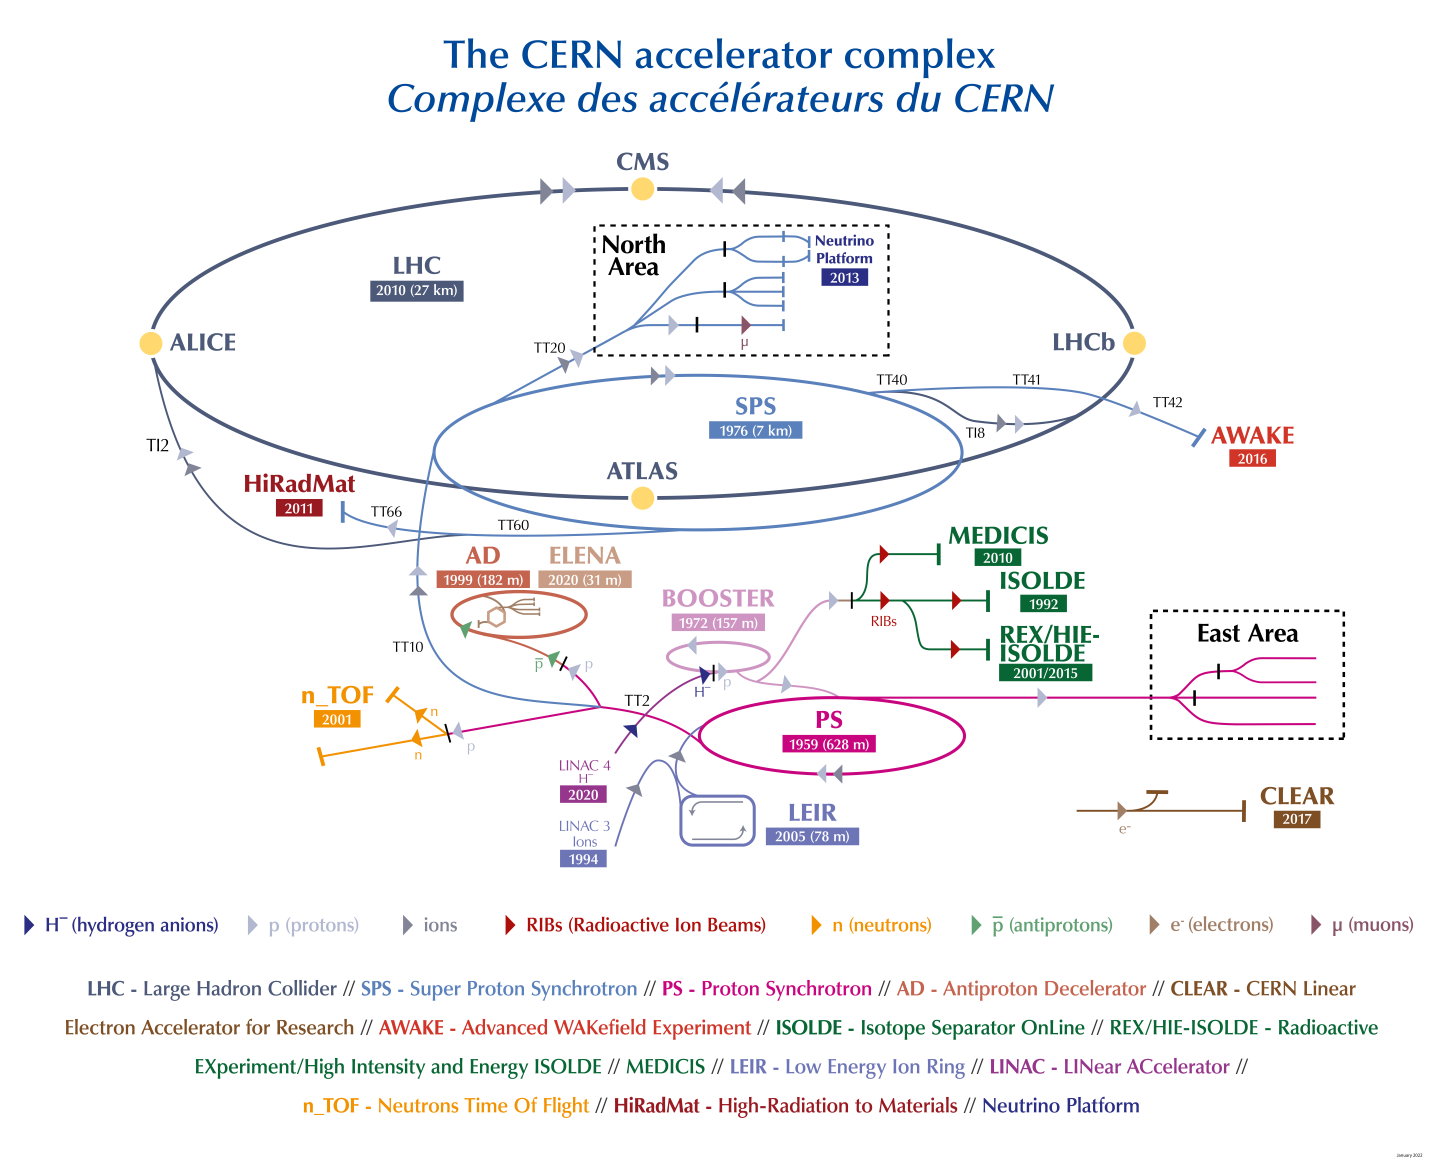
\includegraphics[width=0.75\linewidth]{3_experiment/lhc/AcceleratorComplex2022_large.png}
    \caption{Vista general del complejo de aceleradoes del \ac{LHC}~\cite{LHC-complex}.}
    \label{fig:atlas:lhc:lhc}
\end{figure}

En la \Fig{\ref{fig:atlas:lhc:lhc}} se muestra un esquema general de las instalaciones del acelerador \ac{LHC}. Los protones se obtienen de hidrógeno gaseoso eliminando sus electrones y se aceleran en un primer acelerador lineal (LINAC2) hasta \(50~\mev\). Posteriormente, los protones se aceleran sucesivamente en el \ac{PSB}, el \ac{PSync} y el \ac{SPS}, donde alcanzan una energía de \(450~\gev\) antes de ser inyectados en el \ac{LHC}. En el \ac{LHC}, 8 cavidades de radiofrecuencia pueden impulsar la energía de los protones hasta \(14~\tev\). Los cuatro puntos amarillos en la imagen \Fig{\ref{fig:atlas:lhc:lhc}} son cuatro puntos de interacción entre las part\'iculas acelaradas, que albergan los experimentos \ac{ALICE}~\cite{ALICE}, \acs{LHCb}~\cite{LHCb}, \acs{CMS}~\cite{CMS}, \acs{ATLAS}~\cite{ATLAS}, \acs{LHCf}~\cite{LHCf}, \acs{TOTEM}~\cite{TOTEM}, \acsu{MoEDAL}~\cite{MoEDAL}, entre muchos otros.

Los protones se inyectan en paquetes (\textit{bunches}) de \(\mathcal{O}(10^{11})\) protones en el \ac{LHC} con una separación de 25 ns (7,5 m). Estos haces se llevan posteriormente a colisión en los llamados \textit{bunch-crossing}. El esquema de llenado de la cadena del preacelerador, en combinación con los tiempos de conmutación finitos de los imanes de inyección y descarga, da lugar a patrones regulares de paquetes llenos y vacíos.

% Hasta ahora, el \ac{LHC} ha proporcionado haces de protones e iones pesados durante dos periodos de toma de datos, y se está sometiendo a un tercero. Entre 2009 y 2013 (conocido como \RunOne), el \ac{LHC} operó con una energía de centro de masa ($\sqrt{s}$) de 7 TeV y 8 TeV. Tras la primera larga parada de toma de datos (\ac{LS1}), la segunda corrida (\RunTwo) comenzó en 2015 y finalizó en 2018, proporcionando colisiones de 13 TeV a los experimentos alrededor del anillo \ac{LHC}. En 2022 comenzó el Run-3, en el que se producen \pp colisiones a una energía de \(13.6~\tev\), que se estima durará hasta 2026.



Uno de los parámetros más importantes para caracterizar el funcionamiento del acelerador es la luminosidad instantánea \(\mathcal{L}\), definida como el número de partículas por unidad de tiempo por unidad de \'area, y puede calcularse a partir de la relación
\begin{equation}
    \mathcal{L} = \frac{N_b^ 2n_b f_{rev}\gamma_r}{4\pi\epsilon_n\beta^*}F
    \label{eq:atlas:LHC:instantaneous_lumi}
\end{equation}
donde $N_b$ es el número de partículas por bunch, $n_b$ el número de bunches por haz, $\gamma_r$ es el factor gamma relativista, $\epsilon_n$ es la emitancia transversal normalizada del haz y $\beta^*$ es la función beta en el punto de colisión que determina la dispersión transversal del haz de partículas. El término de corrección F tiene en cuenta el ángulo de cruce del haz. La frecuencia de revolución está representada por $f_{rev}$ que es de \(\sim 11~\)kHz, y con el espaciado del haz de \(25~ns\), permite el cruce del haz en los cuatro puntos de interacción con una frecuencia de \(\sim 40~\)MHz.

La medida para el total de datos registrados se obtiene a partir de la luminosidad integrada a lo largo del tiempo y viene dada por
\begin{equation}
    N_{event} = L_{int} \sigma_{event} = \sigma_{event} \int \mathcal{L} dt.
    \label{eq:atlas:LHC:integrated_lumi}
\end{equation}
Esta variable relaciona la luminosidad con el número de eventos. Más detalles sobre las mediciones de luminosidad en \ac{ATLAS} se muestran en \Sect{\ref{sec:atlas:runs}}.








\FloatBarrier
\section{ATLAS}
\label{sec:atlas:atlas}

\ac{ATLAS} es uno de los detectores multipropósito del \ac{LHC}. Fue diseñado y construido para estudiar las colisiones \pp (y de iones pesados) y un gran espectro de procesos f\'isicos en la escalade energ\'ia del \tev.

La forma general del detector es la de un cilindro, como se muestra en la \Fig{\ref{fig:atlas:atlas:atlas}}. Tiene una longitud de 44 m y 25 m de diámetro, siendo el mayor detector de partículas construido hasta la fecha. El detector \ac{ATLAS} está dividido geométricamente en dos partes: la parte central (\textit{barrel}), y las tapas exteriores (\textit{end-caps}).

\begin{figure}[ht!]
    \centering
    \includegraphics[width=0.8\linewidth]{3_experiment/atlas/ATLAS_full.png}
    \caption{Vista general del detector \ac{ATLAS} y de todos sus subdetectores, incluidos los sistemas añadidos durante el \ac{LS2}~\cite{ATLAS-Diagram}.}
    \label{fig:atlas:atlas:atlas}
\end{figure}

\ac{ATLAS} está construido en capas de subdetectores, cada uno de los cuales está diseñado para tener un papel diferente en la identificación y reconstrucción de las partículas producidas en las colisiones. \ac{ATLAS} proporciona una cobertura hermética alrededor del eje del haz, permitiendo la detección de todas las partículas cargadas generadas en las colisiones en el plano ortogonal al eje del haz. Esto es particularmente importante en las búsquedas de nueva física, que se basan en análisis de balances de momento en el plano ortogonal.

Está formado por múltiples capas, empezando por el componente más interno, el \acf{ID}, que permite reconstruir trazas cerca del tubo del haz. Alrededor del \ac{ID}, hay un solenoide superconductor que crea un campo magnético axial de \(\sim 2\) T para curvar las trazas de las partículas cargadas.
Tras este imán, hay un sistema de dos calorímetros: el \acf{ECAL} y el \acf{HCAL}. El primero se encarga de medir la energía cinética de fotones y electrones, y el segundo mide la energía de los jets.
Las partes más externas del \ac{ATLAS} están constituidas por el \acf{MS}, que proporciona la reconstrucción del momento de los muones que atraviesan las capas internas del detector. Entrelazadas con el \ac{MS}, hay un total de 8 bobinas toroidales que proporcionan un campo magnético total de 4 T para medir el momento de los muones. El campo magnético de los toroides se completa con los toroides en las regiones del end-cap, que también generan un campo magnético de hasta 4 T para los muones que salen en la direcci\'on m\'as pr\'oxima al haz.

% El trabajo conjunto de todos los componentes de \ac{ATLAS} permite reconstruir e identificar una gran variedad de partículas con gran precisión. En la \Tab{\ref{tab:atlas:atlas:expected_performance}}, adaptado de \Refn{\cite{ATLAS}}, se da una visión general de las capacidades de diseño de \ac{ATLAS} en términos de resolución de momento y energía.
% Aquí, la resolución est\'a dada primero por un término estocástico, que mide la incertidumbre basada en la interacción de una partícula con el material, seguido de un término de ruido, que da cuenta de las incertidumbres debidas al ruido electrónico en el proceso de lectura.




% \begin{table}[ht!]
%     \caption{Rendimiento esperado del detector \ac{ATLAS}. Las unidades de \pt y \(E\) están en \gev. Extraído de \Refn{\cite{ATLAS}}}
%     \begin{tabular}{|l|c|c|c|}
%         \hline
%         \multirow{2}{*}{\textbf{Componente del detector}}    & \multirow{2}{*}{\textbf{Resoluci\'on requerida}}     & \multicolumn{2}{c|}{\textbf{Cobertura en $\eta$}}             \\\cline{3-4} 
%                                                         &                                                   & Offline               & Trigger                        \\ \hline
%         \ac{ID}                                        & \( \sigma_{\pt}/\pt = 0.05\%\pt \oplus 1\%    \)  & \( \pm 2.5 \)            &                                \\ \hline
%         \ac{ECAL}                                  & \( \sigma_{E}/E = 10\%/\sqrt{E} \oplus 0.7\%  \)  & \( \pm 3.2 \)            & \( \pm 2.5 \)                  \\ \hline
%         \ac{HCAL} (jets)                     &                                                   &                          &                                \\
%         $\quad$ barrel y end-cap                       & \( \sigma_{E}/E = 50\%/\sqrt{E} \oplus 3\%    \)  & \( \pm 3.2 \)            & \( \pm 3.2 \)                  \\
%         $\quad$ direcci\'on forward                                  & \( \sigma_{E}/E = 100\%/\sqrt{E} \oplus 10\%  \)  & \( 3.1 < \abseta< 4.9 \) & \( 3.1 < \abseta< 4.9 \)       \\ \hline
%         \ac{MS}                               & \( \sigma_{\pt}/\pt = 10\%\) at \(\pt =1~\tev \)  & \( \pm 2.7 \)            & \( \pm 2.4 \)                  \\
%         \hline
%     \end{tabular}
%     \label{tab:atlas:atlas:expected_performance}
% \end{table}







\subsection{Sistema de coordenadas de ATLAS}

\begin{figure}[ht!]
    \centering
    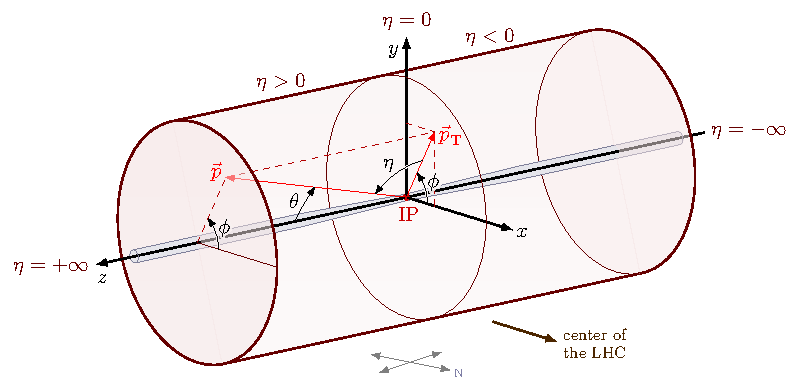
\includegraphics[width=0.8\linewidth]{3_experiment/atlas/ATLAS_coordinates}
    \caption{Sistema de coordenadas de \ac{ATLAS}~\cite{ATLAS-Diagram}.}
    \label{fig:atlas:atlas:atlas_coordinates}
\end{figure}

El sistema de coordenadas utilizado en \ac{ATLAS}, que se muestra en \Fig{\ref{fig:atlas:atlas:atlas_coordinates}}, se utiliza en toda esta tesis y se describe brevemente a continuación~\cite{ATLAS}.
El origen del sistema de coordenadas está en el punto de interacción nominal, con el eje x positivo apuntando hacia el centro del \ac{LHC}. El plano x-y es perpendicular al eje del haz, definiendo el eje z. Hacia la superficie define el eje y positivo. Alrededor del eje del haz se define un ángulo azimutal $\phi$, y un ángulo polar $\theta$ es el ángulo desde el eje del haz. En lugar de $\theta$ se utiliza la rapidez $y$ que para objetos pesados tiene la forma:
\begin{equation}
    y = \frac{1}{2} \ln[(E+p_z)/(E-p_z)].
\end{equation}
Las diferencias en la rapidez son invariantes a \textit{boosts} a lo largo del eje del haz. Para objetos sin masa o relativistas ($m \ll \vb*{p}$) se utiliza en su lugar la pseudorapidez:
\begin{equation}
    \eta = -\ln(\tan(\theta/2)).
\end{equation}
Para cuantificar la distancia entre dos objetos, se define \DeltaR:
\begin{equation}
    \DeltaR = \sqrt{\Delta\phi^2 + \Delta\eta^2}
\end{equation}
El momento transverso y la energía se definen en el plano x-y, con el momento transverso dado como $\pt = \sqrt{p_x^2 +p_y^2}$.






\subsection{Detector Interno}
\label{subsec:atlas:atlas:id}

\begin{figure}[ht!]
    \centering
    \begin{subfigure}[t]{0.49\linewidth}
        \centering
        \includegraphics[width=\linewidth]{3_experiment/atlas/inner_detector.jpg}
        \caption{El \ac{ID} con todos sus submódulos en las regiones de barrel y end-cap.~\cite{ATLAS-InnerDetector}.}
        \label{fig:atlas:atlas:atlas_inner_detector:general}
    \end{subfigure}
    \hfill
    \begin{subfigure}[t]{0.49\linewidth}
        \centering
        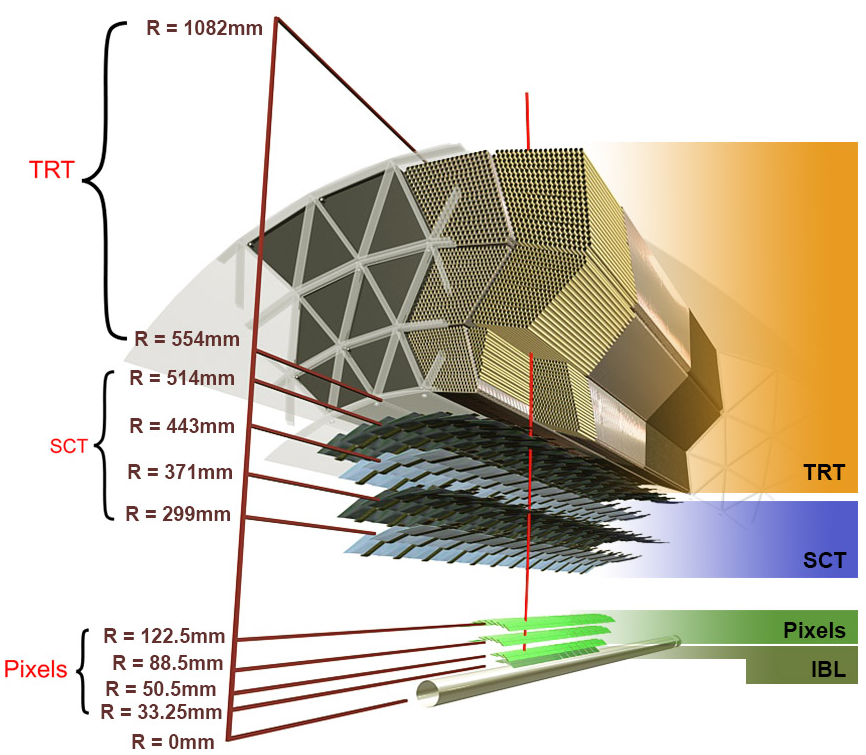
\includegraphics[width=0.8\linewidth]{3_experiment/atlas/inner_detector_layers}
        \caption{Capas del \ac{ID} mostrando su distancia al haz~\cite{ATLAS-InnerDetector}.}
        \label{fig:atlas:atlas:atlas_inner_detector:layer_radius}
    \end{subfigure}
    \caption{Diagramas del \ac{ID} que muestran los diferentes submódulos, con sus correspondientes dimensiones.}
    \label{fig:atlas:atlas:atlas_inner_detector}
\end{figure}

El esquema de un corte transversal del \acf{ID} \cite{ATLAS-ID-TDR} se muestra en la \Fig{\ref{fig:atlas:atlas:atlas_inner_detector}}, resaltando la distancia de cada subsistema respecto al tubo del haz. La parte más interna del \ac{ID} se denomina \ac{IBL}, seguido de tres capas de detectores de píxeles. A 299 mm de distancia radial del tubo del haz, cuatro capas de módulos del \ac{SCT} se sitúan antes del \ac{TRT}, que amplía el tamaño total del \ac{ID} a un radio de 1082 mm. El \ac{ID} permite la reconstrucción de las trazas de partículas en un rango de $\abseta < 2.5$.


La función del \ac{ID} es la reconstrucci\'on de las trazas de las partículas cargadas para determinar su carga y momento. Está inmerso en un campo magnético de 2 T generado por el sistema magnético del solenoide de \ac{ATLAS}, que curva las trayectorias de las partículas cargadas. El radio de curvatura es proporcional al momento de la partícula y su dirección distingue las cargas positivas de las negativas. Las trazas de las partículas detectadas permiten reconstruir los vértices de colisiones primarios, lo cual es importante para distinguir las colisiones de \textit{pile-up} (t\'ermino que ser\'a descrito m\'as adelante) de las colisiones de interés, y los vértices secundarios de decaimiento producidos por partículas de vida media larga, lo que es crucial para la identificación de, por ejemplo, mesones \(B\) o leptones \(\tau\). A continuaci\'on, se brinda una breve descripci\'on de cada parte del \ac{ID}.


\paragraph{\acf{IBL}}
Después del Run-1, durante el \ac{LS1} en el per\'iodo de 2013-2014, el sistema detector de píxeles fue sometido a mantenimiento y actualizaciones. Dentro de este conjunto de actualizaciones, una cuarta capa de píxeles a 3,3 cm de distancia del tubo del haz fue instalada~\cite{ATLAS-IBL-TDR,ATLAS-IBL-proceedings} y ha permitido mejoras significativas en la reconstrucción de vértices de interacción y la identificación de jets iniciados por quarks \(b\).


\paragraph{Detector de P\'ixeles}
La capa de píxeles más interna, el \ac{IBL}, está rodeada por tres capas de detectores de píxeles, dispuestas alrededor del tubo del haz~\cite{ATLAS-Pixel-DesignPerformance,ATLAS-Pixel-Performance-Proceedings}. El método de detección de partículas cargadas es la medición de cargas inducidas depositadas en una capa de silicio, producto de la ionización. La primera capa se encuentra a una distancia de 50,5 mm del centro del tubo del haz. Como se puede ver en la \Fig{\ref{fig:atlas:atlas:atlas_inner_detector:general}}, en la regi\'on del end-cap los detectores de píxeles consisten en 3 discos alrededor del tubo, aumentando la longitud del detector de píxeles del \ac{ID} a 1,4 m a lo largo del eje del haz. El detector de píxeles consta de un total de 1744 módulos de píxeles con un tamaño nominal de $50 ~\mu m \times 400 ~\mu m$ en el plano $(\phi, z)$, que comprenden más de 80 millones de canales de lectura.  
La parte de píxeles y \ac{IBL} del detector \ac{ATLAS} es crucial para la reconstrucci\'on de trazas, ya que proporciona 4 puntos de medici\'on (\textit{hits}) en todo el rango de cobertura de pseudorapidez ($|\eta| < 2.5.$).  

\paragraph{\acf{SCT}}
El detector de píxeles y \ac{IBL} se encuentran dentro de los módulos del \ac{SCT}~\cite{ATLAS-SCT}.  
Al igual que los módulos detectores de píxeles, los módulos del \ac{SCT} están basados en semiconductores, dispuestos en capas cilíndricas alrededor del tubo del haz en la región del barrel, formando discos en los end-caps. Dado que los módulos del \ac{SCT} sólo proporcionan una localización precisa a lo largo de un eje, se combinan dos módulos uno detrás de otro y rotados entre sí para obtener información espacial bidimensional. En el barrel hay cuatro capas y en los end-caps, nueve discos en cada lado (véase la \Fig{\ref{fig:atlas:atlas:atlas_inner_detector:general}}). Incluyendo los discos de los end-caps, el \ac{SCT} se extiende hasta $|z| < 2735~mm$.

\paragraph{\acf{TRT}}
La última parte del \ac{ID} es el \ac{TRT}~\cite{ATLAS-TRT-DesignPerformance}, el cual en la regi\'on barrel se extiende de 554 mm a 1082 mm de distancia radial. Este detector se compone de tubos detectores de 4 mm de diámetro, dispuestos en paralelo al tubo del haz en la regi\'on barrel, y radialmente en los end-caps. En el rango de $|\eta| < 2.0$, se sit\'uan tres anillos en el barrel y 18 unidades en los end-caps, proporcionando típicamente 36 impactos por traza. Los tubos están entrelazadas con fibras de polipropileno, que cuando las part\'iculas las atraviesan, crean la radiación de transición. En el interior de los tubos hay un fino cable de tungsteno que recoge las cargas. El nivel de radiación y las cargas recogidas en cada tubo pueden utilizarse para discriminar entre electrones y piones cargados. El \ac{TRT} sólo ofrece información espacial en el plano $(R-\phi)$, y no se puede extraer información en la dirección z debido a la orientación de estos tubos. Hay un total de aproximadamente 50000 tubos en la región del barrel, mientras que en los end-caps se sit\'uan aproximadamente 250000 tubos.








\subsection{Calor\'imetros}

\begin{figure}[ht!]
    \centering
    \includegraphics[width=0.8\linewidth]{3_experiment/atlas/calorimenters.jpg}
    \caption{Sistema de calor\'imetros de \ac{ATLAS}, mostrando el \acf{ECAL} y el \acf{HCAL}~\cite{ATLAS-Calorimeter-Diagram}.}
    \label{fig:atlas:atlas:atlas_calorimeters}
\end{figure}

El sistema \ac{ID} está rodeado por dos calorímetros: el \acf{ECAL} y el \acf{HCAL}, como se muestra en la \Fig{\ref{fig:atlas:atlas:atlas_calorimeters}}. Estos calorímetros están diseñados para medir la energía y la posición de las partículas incidentes, a través de la energía depositada por las cascadas de partículas secundarias producidas por las incidentes. Cubre todo el rango \(\phi\) y hasta el \(\abseta<4.9\), con una granularidad más fina en la región que coincide con el \ac{ID}.
El sistema de calorímetro permite discriminar entre fotones y electrones de hadrones (jets). Además, permite medir el desequilibrio energético (gracias a su cobertura total y hermiticidad) y proporciona al sistema de trigger la información necesaria para la selección de eventos.

Ambos calorímetros son denominados calorímetros de muestreo, con capas alternas de material absorbente y activo. La capa absorbente desencadena una lluvia de part\'iculas consecutivas con el material detector, la capa activa detecta la señal.
El desarrollo de la lluvia y sus propiedades son de vital importancia para la identificación de las partículas, como se verá más adelante.
Dos magnitudes importantes en relación con los calorímetros son la longitud de radiación, $X_0$, y la longitud de interacción $\lambda$. La longitud de radiación se refiere a la distancia después de la cual la energía de una partícula (electrones por ejemplo) se ha reducido a \(1/e\) de su energía inicial. La longitud de interacción describe el camino libre medio antes de que se produzca una interacción hadrónica.

La resolución de diseño del sistema sobre la energía calorimétrica viene dada por
\begin{equation}
    \frac{\sigma(E)}{E} = 
    \frac{a}{\sqrt{E}} \oplus b \oplus \frac{c}{E}
\end{equation}
donde \(\oplus\) significa que los términos se suman en cuadratura. El término estocástico \(\frac{a}{\sqrt{E}}\) está relacionado con las fluctuaciones en los desarrollos de la lluvia, el término constante \(b\) tiene en cuenta las inhomogeneidades del detector, y el último término está asociado con el ruido electrónico y es proporcional a \(\frac{1}{E}\). El valor de los coeficientes \(a\) y \(b\) depende de los objetos incidentes. Para el caso de los electrones en el \ac{ECAL}, \(a\sim 10\%~\gev^{1/2}\) y \(b~\sim 0.7\%\), mientras que los de los piones cargados en el centro del detector son \(a~\sim50\%~\gev^{1/2}\) y \(b\sim5\%\) \cite{ATLAS-Calorimeters-PerformanceRun2}.



\subsubsection{\acf{ECAL}}
\label{subsubsec:atlas:atlas:cals:ecal}

El \ac{ECAL} está especializado en la detección de electrones, positrones y fotones, que depositan su energía en lluvias relativamente densas: electrones energéticos que irradian fotones Bremsstrahlung, mientras que los fotones energéticos se convierten en pares electrón-positrón al atravesar el material denso.
El material absorbente está hecho de plomo (Pb) con láminas de acero inoxidable, mientras que el \ac{LAr} se utiliza como material activo con electrodos de cobre y kapt\'on para la lectura.


El calorímetro tiene una geometría de acordeón que proporciona una simetría completa \(\phi\) sin fisuras azimutales.
Está dividido en dos medios barriles que cubren la región central del detector (\(\abseta<1.475\)), con un pequeño hueco (4 mm) en $z = 0$ y una tapa final a cada lado del haz (\(1.375<\abseta<3.2\)).
La región de transición entre el barrel y end-cap se denomina región \textit{crack}, y la mayoría de los análisis físicos que utilizan el \ac{ECAL} requieren que los fotones y electrones se encuentren fuera de ella.
Además el \ac{LAr} se utiliza para las tapas de los calorímetros hadrónicos, así como en el \acf{FCAL} ($3.1 < \eta < 4.9$).

El grosor de \ac{ECAL} es superior a 22 longitudes de radiación (\(X_0\)) en la región del barrel, mientras que es superior a \(24 X_0\) en la región de end-caps. En el caso de los fotones, la distancia a la que la energía baja a \(1/e\) es de \(9/7 X_0\), por lo que toda la energía electromagnética del fotón se deposita en el \ac{ECAL}, y sólo una pequeña parte llega al \ac{HCAL}.

El modo de medición es el siguiente. Las partículas incidentes interactúan con el medio absorbente (Pb), iniciando una lluvia de partículas cargadas y neutras. Las partículas cargadas ionizan el \ac{LAr} y los electrodos recogen los electrones producidos en el proceso de ionización. La señal total del medio activo es entonces proporcional a la energía real total de la partícula incidente.

\begin{figure}[ht!]
    \centering
    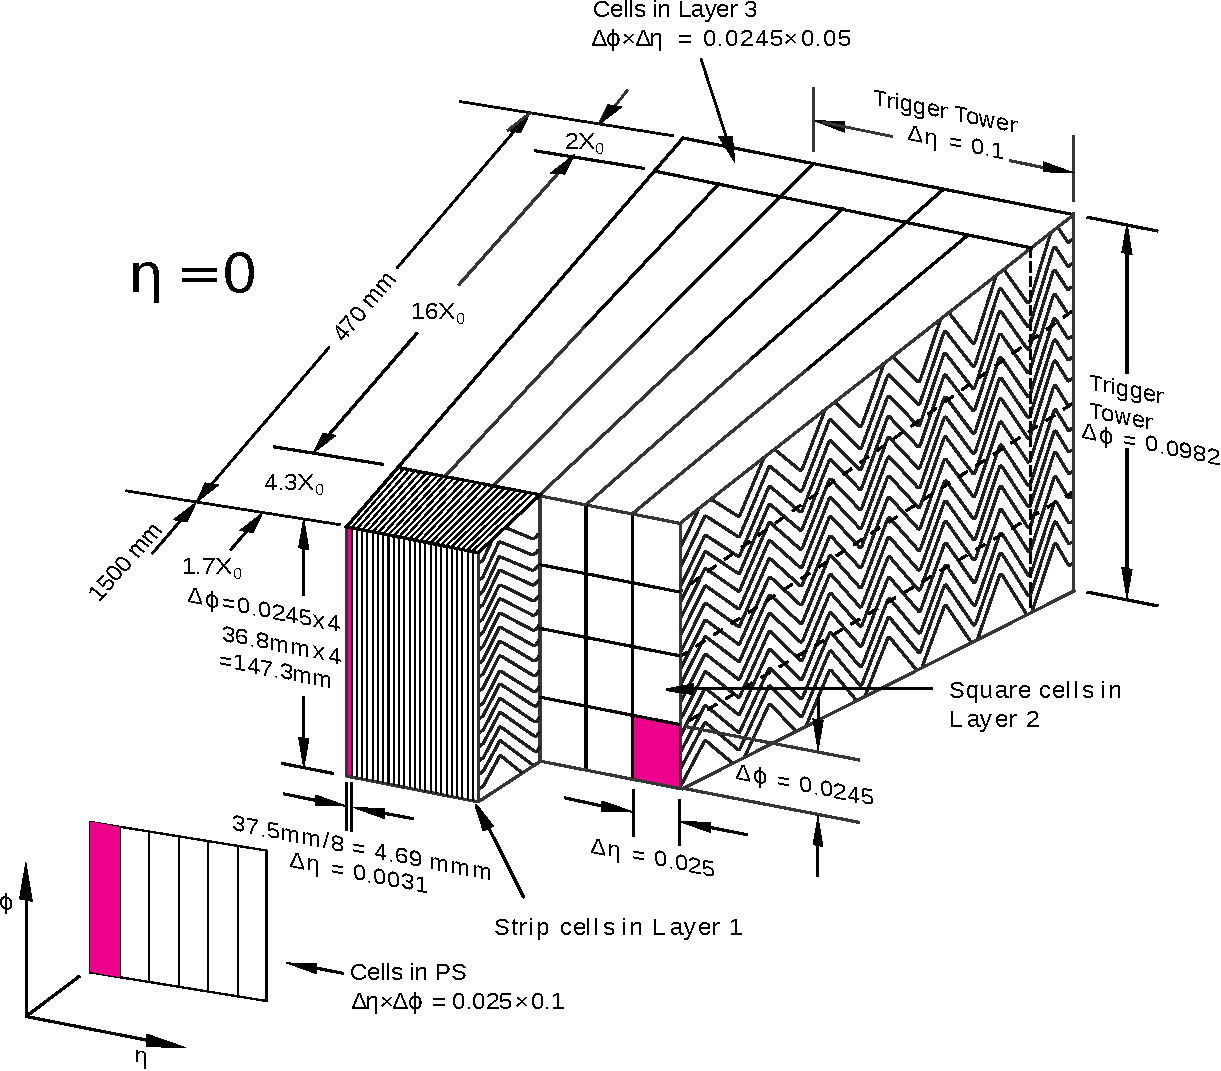
\includegraphics[width=0.8\linewidth]{3_experiment/atlas/ecal_cells}
    \caption{Segmento del \ac{ECAL} mostrando la disposici\'on de las capas y celdas del calor\'imetro. Adem\'as, se muestran las dimensiones de las celdas en cada capa~\cite{ATLAS}.}
    \label{fig:atlas:atlas:cals:ecal:ecal_cells}
\end{figure}

\begin{figure}[ht!]
    \centering
    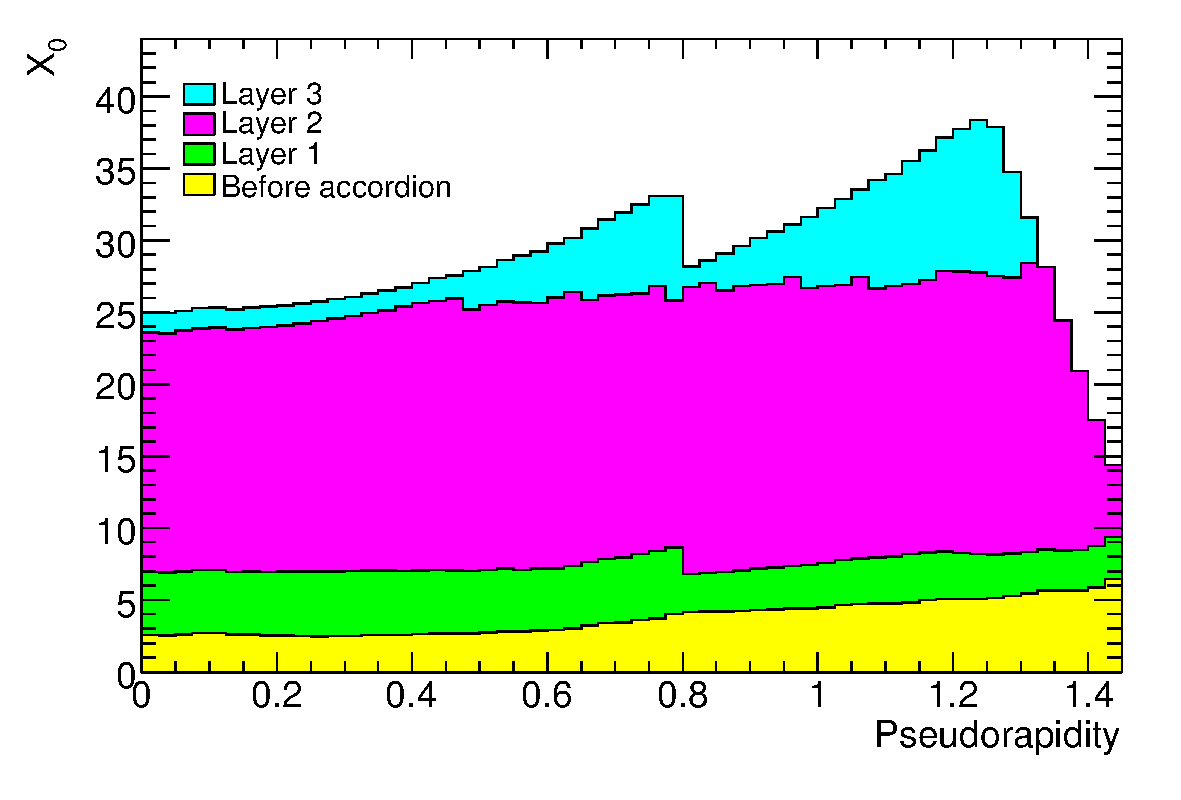
\includegraphics[width=0.46\linewidth]{3_experiment/atlas/ecal_radiation_lengths1}
    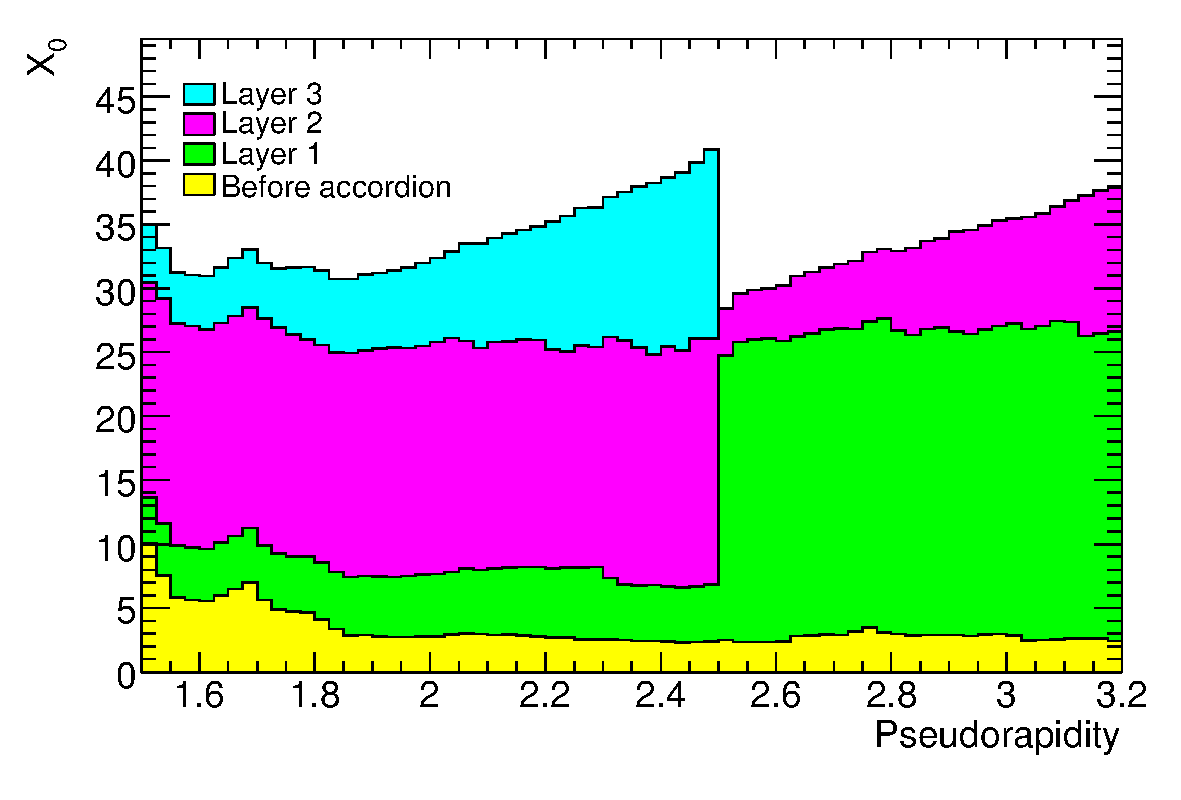
\includegraphics[width=0.46\linewidth]{3_experiment/atlas/ecal_radiation_lengths2}
    \caption{Longitudes de radiaci\'on en funci\'on de \abseta para cada capa del \ac{ECAL}~\cite{ATLAS}.}
    \label{fig:atlas:atlas:cals:ecal:ecal_radiation_length}
\end{figure}

Dentro de la región aceptada para las medidas de precisión (\(\abseta<2.5\) excluyendo el crack), el \ac{ECAL} se segmenta en tres capas longitudinales, mostradas en la \Fig{\ref{fig:atlas:atlas:cals:ecal:ecal_cells}}.
La primera capa consiste en bandas de granularidad fina (también llamada \textit{strip layer}) que ayuda a discriminar entre fotones aislados y pares de fotones espacialmente cercanos procedentes de decaimientos \(\pizero\to\gamma\gamma\). Esta capa tiene un espesor constante de \(\sim 6 X_0\) en función de \(\eta\) (véase la \Fig{\ref{fig:atlas:atlas:cals:ecal:ecal_radiation_length}}), y proporciona una medida precisa de \(\eta\).
Para los fotones y electrones de alta energía, la mayor parte de su energía se recoge en la segunda capa, que tiene una granularidad lateral de \(0.025 \times 0.025\) en \((\eta, \phi)\) y un espesor de \(\sim 24 X_0\).
La tercera capa recoge la energía depositada por las colas de la lluvia electromagnética, con un espesor que varía entre 2 y 12 \(X_0\).
También hay un \textit{presampler} (no se muestra en las figuras), que cubre la región \(\abseta<1.8\) que mejora la medición de la energía para las partículas que comienzan la lluvia antes de entrar en el calorímetro.




\subsubsection{\acf{HCAL}}



Tres capas de calorímetro hadrónico rodean el \ac{ECAL} y proporcionan discriminación adicional para electrones y fotones al medir la energía hadrónica. El \ac{HCAL} se extiende en pseudorapidez hasta \(\abseta<4.9\), permitiendo cubrir prácticamente la totalidad del ángulo sólido desde el punto de interacción. En la región del barrel (\(\abseta<1.7\)) se encuentra el primer calorímetro, el \textit{Tile calorimeter}, un calorímetro de muestreo que utiliza acero como material absorbente y tejas centelladoras como material activo~\cite{ATLAS-Tile-TDR}. Está dividido en dos parte: \(\abseta<1.0\) y \(0.8<\abseta<1.7\). Las tejas centelleadoras est\'an dispuestas de una forma periódica y están conectadas a una fibra óptica que transporta la luz producida por las partículas que pasan a un tubo fotomultiplicador. Este arreglo se extiende, en \(R\), de 2.28 a 4.25 m. En la región del end-cap (\(1.5<\abseta<3.2\)) hay un calorímetro de muestreo hadrónico, el \acf{HEC}, con placas de cobre como absorbente y argón líquido como material activo. Cada lado del endcap consiste en dos ruedas, una detrás de la otra con las placas planas de Cu dispuestas perpendicularmente al eje del haz, con un radio de 2.3 m. Finalmente está el \ac{FCAL}, un calorímetro de muestreo que extiende la cobertura del sistema hasta \(\abseta<4.9\), coaxial al eje del haz y situado a 4.7 m a cada lado del punto de interacción. El material principal de los módulos es el \ac{LAr} (con cobre o tungsteno), y aunque no se utiliza para mediciones de precisión, proporciona información para el cálculo de la energía transversa faltante y la reconstrucción de jets en regiones muy cercanas al eje del haz.

El \ac{HCAL} tiene un espesor superior a \(7.7~\lambda\) en la región del barrel (\(9.7~\lambda\) en total si se cuenta el \ac{ECAL}). Análogamente a la longitud de radiación mencionada para el \ac{ECAL}, se puede definir la longitud de interacción hadrónica como la distancia media a lo largo de la cual la energía de un hadrón se reduce a \(1/e\) de su energía inicial. Así, toda la energía con la que los hadrones llegan al \ac{HCAL} se deposita allí.





\subsection{\acf{MS}}

\begin{figure}[ht!]
    \centering
    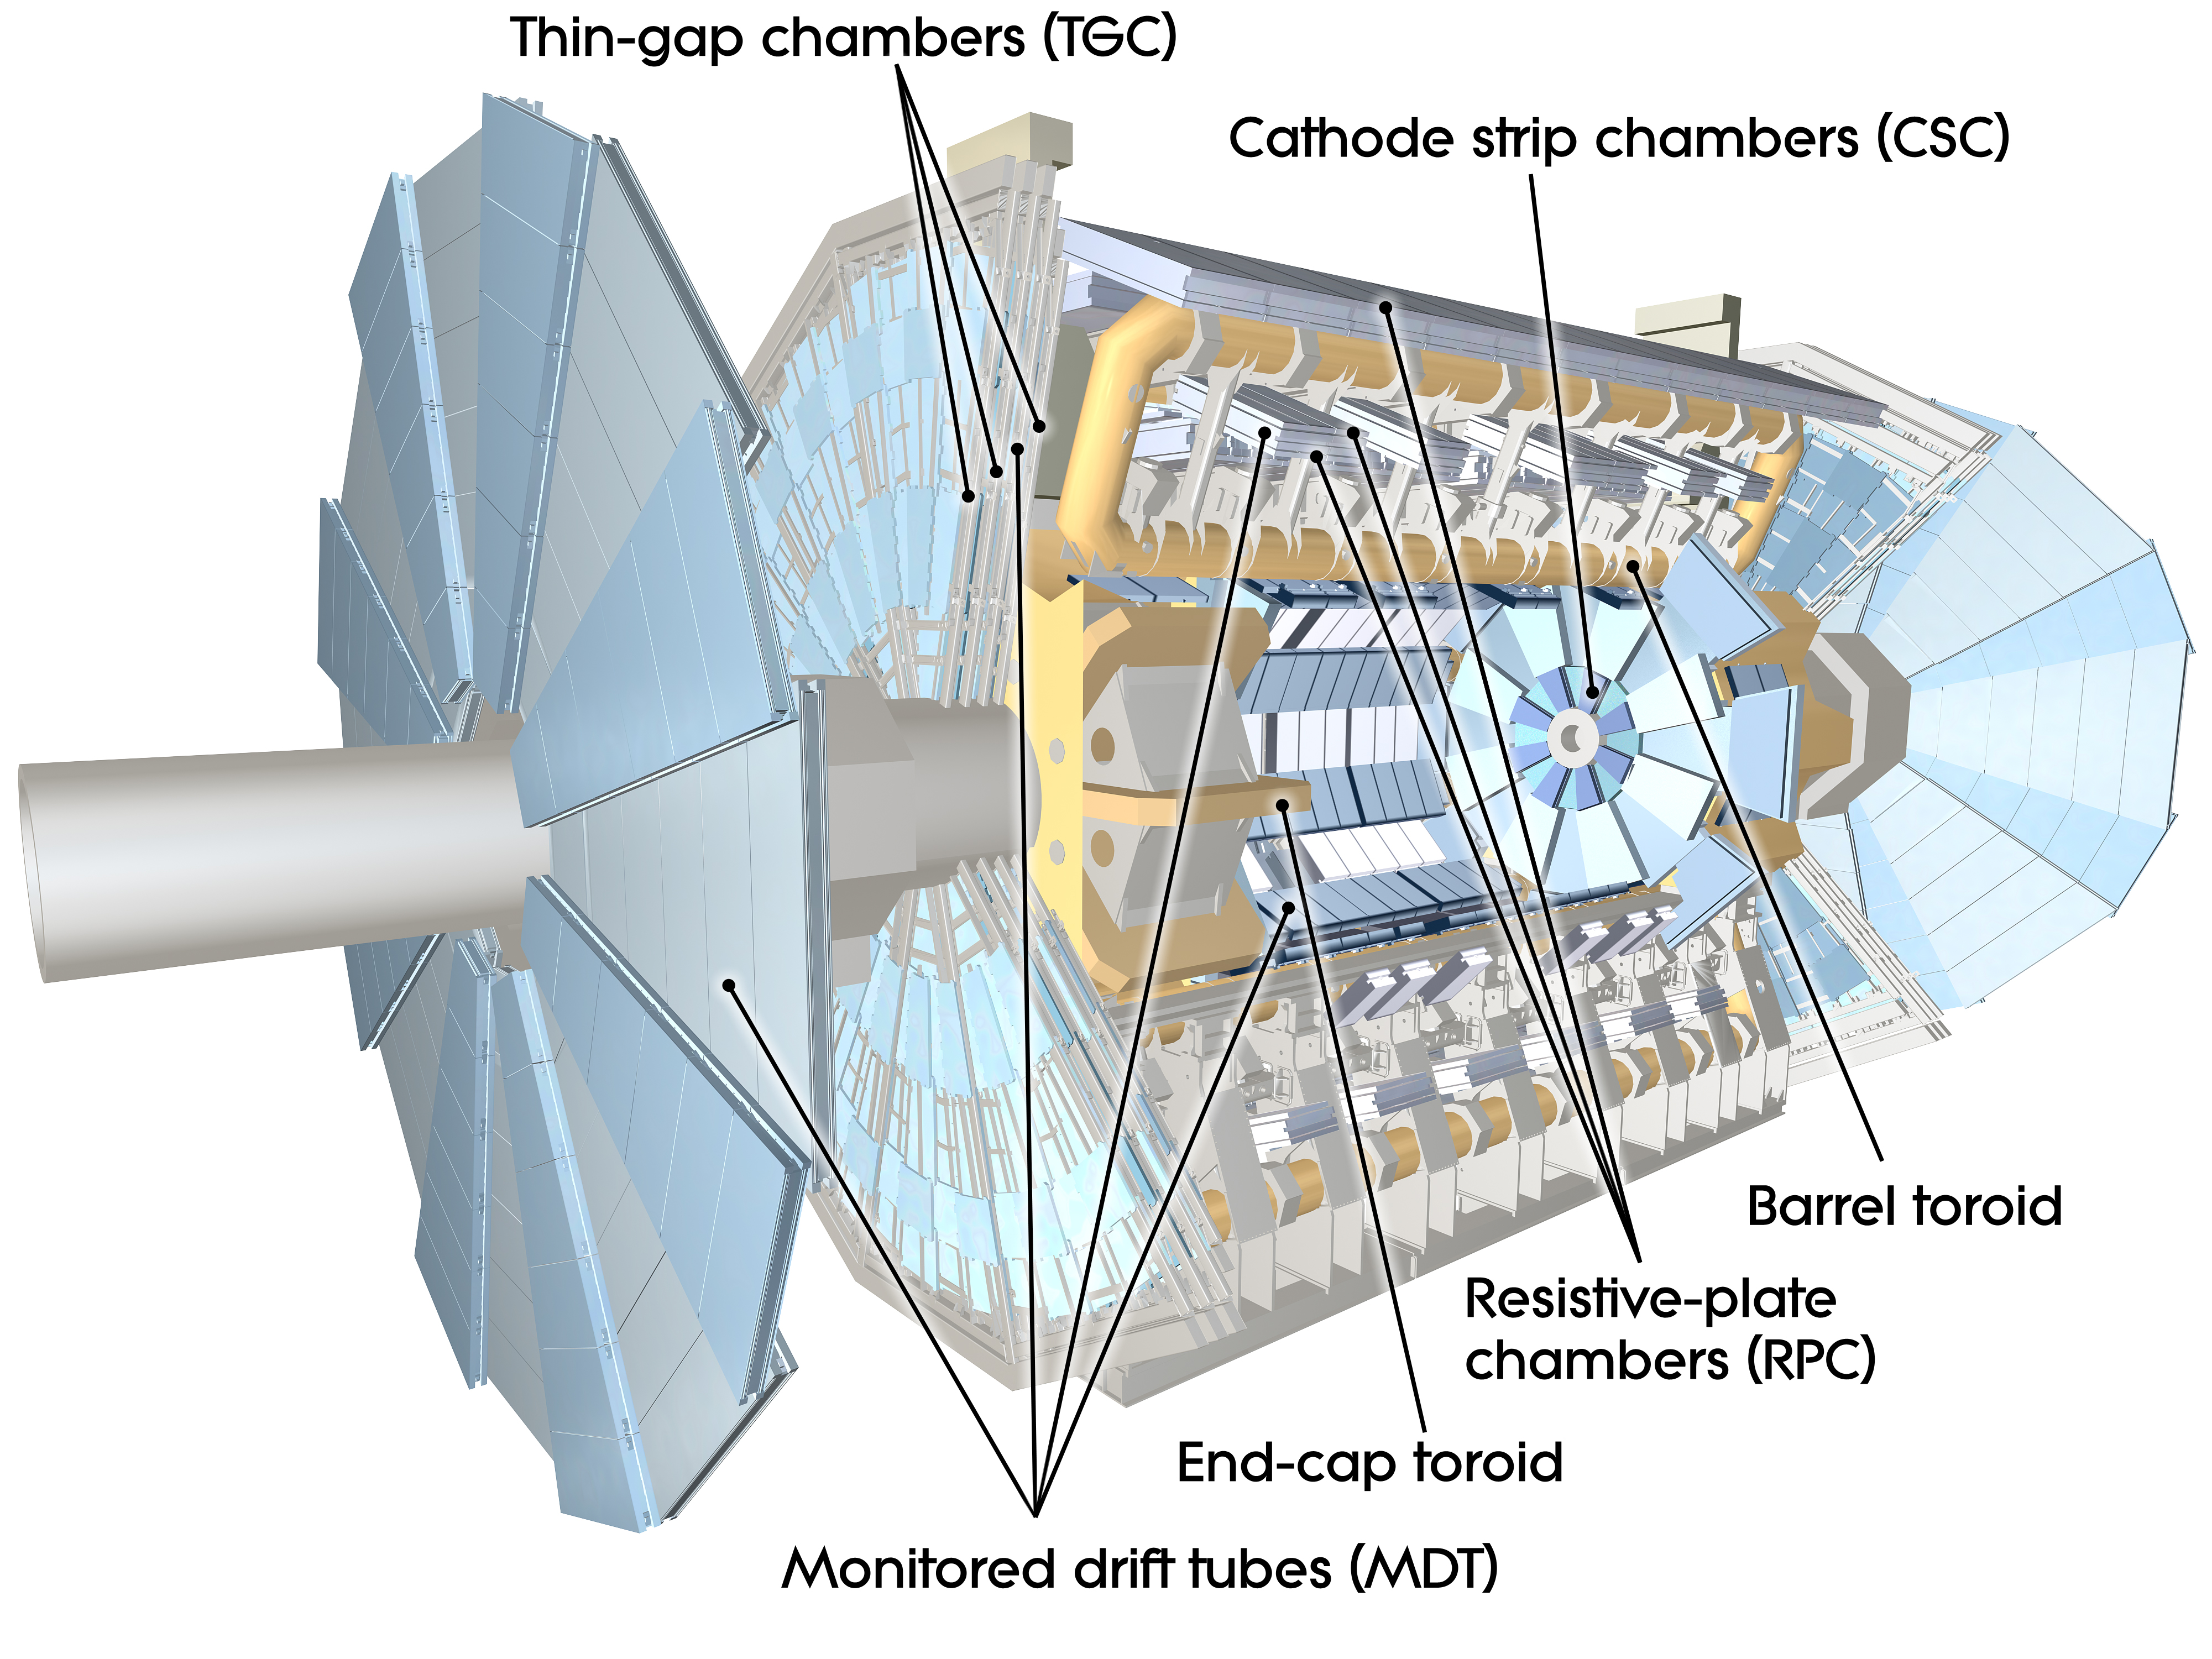
\includegraphics[width=0.6\linewidth]{3_experiment/atlas/muon_detector}
    \caption{Diagrama del \acf{MS}~\cite{ATLAS}.}
    \label{fig:atlas:atlas:muon_spectrometer:muon_spectrometer}
\end{figure}

Los muones de alto \pt generados en el punto de interacción tienen un poder de penetración muy elevado y son poco interactivos. Por lo tanto, el \ac{MS} \cite{ATLAS-Muon-TDR} está situado en la parte más externa del detector \ac{ATLAS}, insertado dentro del campo magnético de 4 T generado por los imanes toroidales del barrel y end-caps, y está diseñado para obtener medidas de posición y momento con alta precisión de los muones de alto \pt en un rango de \abseta de \(\abseta<2.7\). Se trata del mayor subdetector y el que da a \ac{ATLAS} su tamaño. Este subdetector se muestra en la \Fig{\ref{fig:atlas:atlas:muon_spectrometer:muon_spectrometer}}, destacando los subsistemas.

El \ac{MS} se compone de diferentes tipos de cámaras de detección (véase la \Fig{\ref{fig:atlas:atlas:muon_spectrometer:muon_spectrometer}}). Los \acp{MDT} son responsables de la mayoría de las medidas de precisión y cubren el rango de pseudorapidez hasta \(\abseta<2.7\). Funcionan de forma similar al \ac{TRT}, con tubos llenos de un gas ionizante y un ánodo central que recoge los electrones producidos, y el tiempo de deriva está asociado a la distancia a la traza dejada por la part\'icula. En la región del endcap se encuentran las \acp{CSC} que tienen una alta resolución espaciotemporal y una cobertura de \(\abseta>2.0\). Estas cámaras funcionan midiendo la carga depositada en un ánodo como resultado de la cascada de electrones creada cerca de \'el. Las \acp{RPC} proporcionan una estimación rápida del momento de los muones a nivel de trigger con una cobertura de \(\abseta<1.05\)\footnote{Durante el \ac{LS2}, la capa del end-cap ma\'s interna ha sido reemplazada por las \acp{NSW}~\cite{ATLAS-NSW}. Presenta MicroMegas como rastreadores de precisión ya que proporcionan un mejor rendimiento a las altas tasas esperadas en las futuras operaciones del LHC.}. Las \acp{RPC} miden la descarga entre dos placas resistivas paralelas sometidas a una elevada diferencia de potencial, siguiendo la ionización del volumen de gas interno causada por el paso de muones energéticos. Por último, en la región del endcap, se encuentran los \acp{TGC}, de función similar a los \acp{CSC}. También proporcionan información al sistema de trigger en esta región y tienen una cobertura de \(\abseta<2.4\).

Si los hits en el \ac{ID} y el \ac{MS} se pueden asociar a un solo muón, se obtiene una muy buena resolución del momento de hasta
\begin{equation}
    \frac{\sigma(\pt)}{\pt} = 
    0.02\% \cdot \pt~[\gev] \oplus 2\%,
\end{equation}
la cual se degrada si sólo se identifica una traza en uno de los dos sistemas.






\subsection{El sistema de Trigger}



El sistema de trigger de \ac{ATLAS}~\cite{ATLAS-Trigger-Performance-2010,ATLAS-Trigger-Performance-2015,ATLAS-Trigger-Performance-Run2} utiliza información del detector para rechazar eventos que no son de inter\'es para el programa de \ac{ATLAS} (colisiones \textit{soft}, por ejemplo), reduciendo la frecuencia de eventos de 40 MHz (frecuencia de cruce de bunches mencionada en la \Sect{\ref{sec:atlas:LHC}}) a alrededor de 1.5 kHz. Es necesario enfatizar aquí el papel central del sistema de trigger para el correcto funcionamiento de todo el experimento, siendo el responsable de decidir qué eventos se almacenan para su posterior an\'alisis, que podr\'ia llevar, por ejemplo, a un descubrimiento. Para lograr tal reducción en la frecuencia de eventos y, al mismo tiempo, tener una alta eficiencia en la selección de los de interés, el sistema de trigger se compone de dos niveles consecutivos capaces de realizar una identificación de partículas cada vez más compleja; un primer nivel de trigger basado en hardware, el \acf{L1}, y luego un trigger de alto nivel basado en software, el \acf{HLT}. Cada nivel permite analizar los eventos con mayor detalle, aumentando la precisión de los criterios de selección y la complejidad de los algoritmos utilizados.


\subsubsection{\acf{L1}}

La decisión del trigger comienza con el \ac{L1}, basado en hardware~\cite{ATLAS-L1Trigger}, que identifica lo que se conoce como \ac{ROI}. La \ac{ROI} consiste en celdas vecinas en los \ac{ECAL} y \ac{HCAL}, y se define a partir de la posición en el calorímetro de cada objeto encontrado en un evento potencialmente interesante, que se extiende como un cono desde el punto de interacción a lo largo del detector.
En cuanto a los muones, toma la información leída por el \ac{MS}, más concretamente por el \ac{TGC} y el \ac{RPC}, y permite obtener una estimación rápida del \pt del muón.
El \ac{L1} también tiene una componente que permite tener en cuenta los requisitos topológicos, como las selecciones de masa invariante y las medidas de distancia, denominado el \ac{L1Topo}.

El diseño del \ac{L1} permite tener una aceptabilidad en el rango de \(\abseta<2.5\) para electrones, fotones, muones y taus, hasta \(\abseta<3.2\) para jets, y \(\abseta<4.9\) para el cálculo del momento transverso faltante.
Utilizando las \acp{ROI}, el trigger \ac{L1} debe tomar la decisión de guardar o descartar el evento, reduciendo la tasa de eventos de 40 MHz a menos de 100 kHz en aproximadamente \(2.5~\mu s\), tiempo determinado en parte por el tamaño limitado de los buffers de memoria y en parte por el tiempo que tardan los muones producidos en el evento en llegar al \ac{MS}. Esta decisión final la toma el \ac{CTP}, y luego pasa las \acp{ROI} al siguiente nivel de trigger: el \ac{HLT}.



\subsubsection{\acf{HLT}}


Cuando un evento es aceptado por el \ac{L1}, el \ac{HLT}~\cite{ATLAS-HLTTrigger} ejecuta una secuencia de algoritmos a partir de las \acp{ROI} definidas por el \ac{L1}, y permite reducir la tasa de eventos que se almacena a 1.5 kHz en 0.2 s.
La reconstrucción e identificación de partículas candidatas en el \ac{HLT} se evalúa en una secuencia de pasos donde se aplican diferentes algoritmos.
Si la selección falla en un determinado paso, los pasos siguientes ya no se ejecutan para ahorrar tiempo de ejecución.
En el \ac{HLT}, los algoritmos se agrupan en conjuntos de algoritmos de reconstrucción rápida que se ejecutan en primer lugar y, a continuación, se ejecuta un conjunto de algoritmos de reconstrucción de precisión similares a los utilizados \textit{offline}.
Los algoritmos de reconstrucción rápida utilizan la información del calorímetro y de las trazas del \ac{ID} sólo dentro de la \ac{ROI} para realizar la selección e identificación de candidatos, y llevar a cabo el rechazo del fondo lo más rápido posible.
Si la partícula candidata supera los criterios definidos por la selección de reconstrucción rápida, se ejecutan los algoritmos de selección de precisión. Estos tienen acceso a la información del detector fuera de la \ac{ROI}, con la máxima granularidad e incluyendo detalles sobre la calibración energética del calorímetro, la alineación del subdetector y el mapeo del campo magnético.

La secuencia exacta y el tipo de algoritmos considerados en el \ac{HLT} se definen en el \textit{menu} del trigger. Esto comprende una base de datos de triggers, cada uno de los cuales define una secuencia de algoritmos y los requisitos de estos algoritmos para que un evento pase el \ac{HLT}.

Los requisitos de trigger se diseñan de forma tal que la tasa global del \ac{HLT} no supere 1 kHz. En algunos casos, incluso la reducción de la tasa de eventos conseguida mediante los algoritmos del \ac{HLT} para los requisitos de trigger deseados, como los trigger para objetos con bajo momento, es demasiado alta. Para mantener la tasa general del \ac{HLT} por debajo de 1 kHz en estos casos, los triggers pueden seguir incluyéndose en el menú, pero con una preescala. Un preescalado es un escalado artificial del trigger, que sólo acepta la N-\'esima decisión de trigger si el factor de preescalado es N. Esto permite que los triggers con una alta tasa sigan recogiendo eventos.

Los algoritmos del \ac{HLT} se ejecutan en aproximadamente 40.000 núcleos de CPU. Además, la construcción parcial de eventos se utiliza para análisis a nivel de trigger, para el monitoreo del detector y las calibraciones del subsistema detector. Finalmente, los eventos aceptados por el \ac{HLT} se almacenan y se distribuyen, disponibles \textit{offline} para cualquier estudio o análisis.






\FloatBarrier
\section{Toma de datos durante el Run-2}
\label{sec:atlas:runs}


El funcionamiento del \ac{LHC} se organiza en distintos per\'iodos conocidos como \textit{runs}.
% Cada run suele durar varios años y se caracteriza por condiciones experimentales específicas, como la energía a la que colisionan los protones y la intensidad de los haces.
Desde su puesta en marcha, se pueden distinguir los siguientes runs: Run-1 (2010-2013) operó a energías de colisión de hasta 8 TeV, Run-2 (2015-2018) a 13 TeV, y Run-3 (2022-presente) a 13,6 TeV. Cada per\'iodo de toma de datos, una vez que el \ac{LHC} anuncia haces estables, se divide en \ac{LB} de aproximadamente dos minutos. En cada \ac{LB}, la luminosidad instantánea es prácticamente constante y las condiciones del haz son estables. Debido a la alta complejidad del \ac{LHC} y del detector \ac{ATLAS}, se espera que haya ineficiencias en los detectores y subdetectores y/o en la cadena de adquisición de datos. Durante cada run, cada parte del \ac{ATLAS} es monitoreada y cualquier falla o problema es registrado, incluyendo componentes inactivos, o problemas en el haz del \ac{LHC}.

Para garantizar la alta calidad de los datos, libres de defectos significativos, los \ac{LB} y los rangos dentro de ellos que superan todos los criterios de calidad se compilan en \ac{GRL}. Las listas se elaboran y distribuyen de forma centralizada, con el fin de proporcionar a cualquier grupo de \ac{ATLAS} la misma colección de \acp{LB}. Dado que durante los per\'iodos de tomas de datos están disponibles diferentes partes del detector (en un run óptimo, todos los subdetectores están disponibles), hay múltiples \acp{GRL} disponibles para utilizar. Cada análisis, entonces, selecciona qué \ac{GRL} utilizar dependiendo de su tolerancia a las fallas de los subdetectores.

La presente tesis utiliza datos recolectados por \ac{ATLAS} de colisiones \pp del \ac{LHC} durante el Run-2 (2015-2018), a una energía del centro de masa de \(\sqrt{s} = 13~\tev\). Durante este run, el \ac{LHC} entreg\'o un total de \(156~\ifb\), de los cuales \ac{ATLAS} recolect\'o \(147~\ifb\). La luminosidad integrada total disponible para análisis de f\'isica es de \(140.07~\ifb\)\footnote{Las primeras medidas y \ac{GRL} iniciales s\'olo brindaban un total de \(139~\ifb\) disponibles para an\'alisis}, como se ve en la \Fig{\ref{fig:atlas:runs:lumi_run2}}. La incertidumbre en la luminosidad integrada combinada para el Run-2 es de \(0.83\%\)~\cite{ATLAS-Lumi-Run2}, obtenida usando el detector LUCID-2~\cite{ATLAS-LUCID2}.
Hasta el momento, combinando los años 2022, 2023 y 2024 de toma de datos del Run-3, se recogieron 159 \ifb de datos, mostrados en la \Fig{\ref{fig:atlas:runs:lumi_run3}}~\cite{ATLAS-Lumi-Run3-2022,ATLAS-Lumi-Run3-2023}.

\begin{figure}[ht!]
    \centering
    \begin{subfigure}[h]{0.46\linewidth}
        \centering
        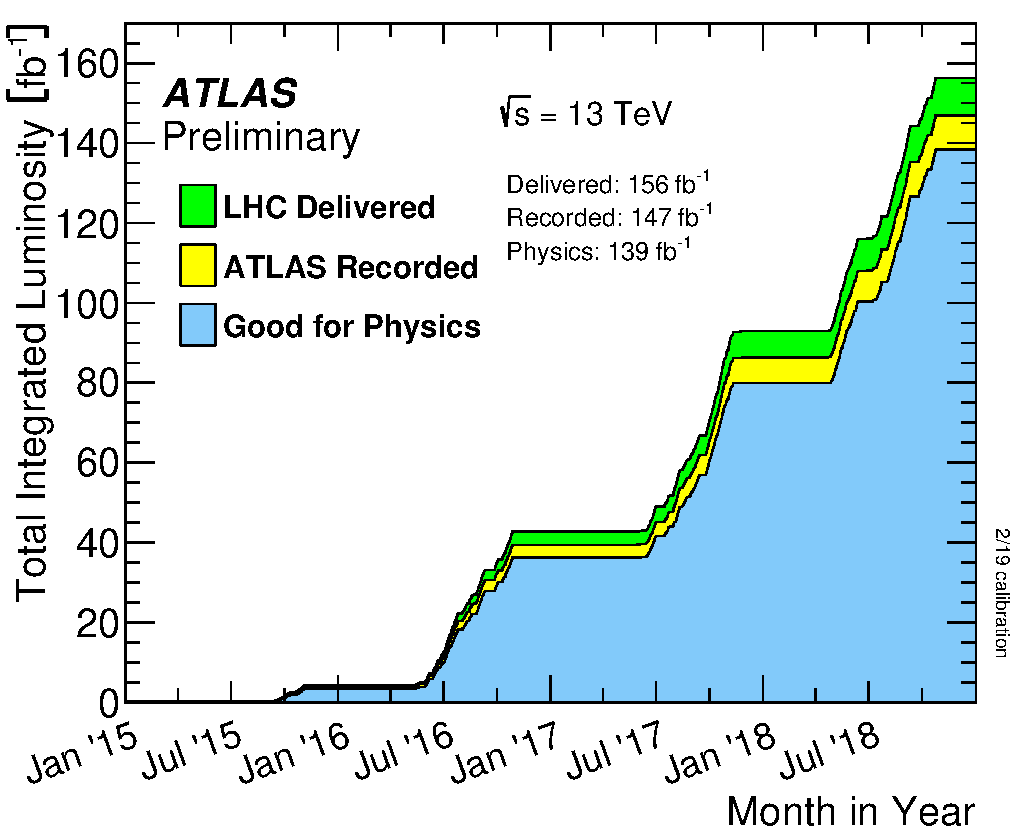
\includegraphics[width=\linewidth]{3_experiment/lhc/DeliveredLuminosityRun2}
        \caption{Run-2 (2015-2018)}
        \label{fig:atlas:runs:lumi_run2}
    \end{subfigure}
    \hfill
    \begin{subfigure}[h]{0.46\linewidth}
        \centering
        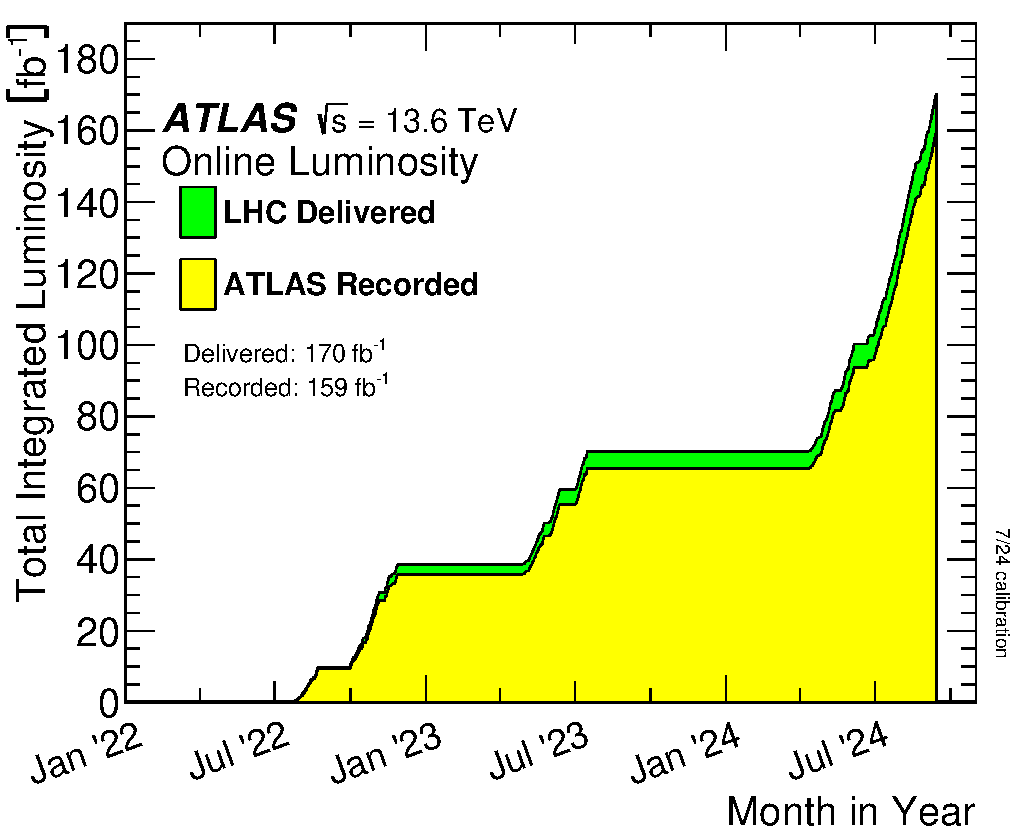
\includegraphics[width=\linewidth]{3_experiment/lhc/DeliveredLuminosityRun3}
        \caption{Early Run-3 (2022-2024)}
        \label{fig:atlas:runs:lumi_run3}
    \end{subfigure}
    \caption{Luminosidad entregada por el \ac{LHC} y recolectada por \ac{ATLAS} durante el Run-2~\cite{ATLAS-Lumi-Run2} y el Run-3. En el caso de Run-2, tambi\'en se muestra la fracci\'on de datos recolectados que son \'utiles para an\'alisis de f\'isica.}
    \label{fig:atlas:runs:lumi}
\end{figure}

Otro concepto importante en la adquisición de datos en \ac{ATLAS} es el \textit{pileup}, que se produce cuando las partículas producidas en más de una colisión \pp llegan al detector al mismo tiempo, o más generalmente, cuando las señales se solapan de forma que no pueden separarse. Cuando colisionan haces de protones, la probabilidad de que se produzca una interacción es proporcional a la densidad de partículas, o mejor, al flujo de partículas, que se expresa mediante la luminosidad instantánea. El número real de colisiones de partículas que tienen lugar cuando dos haces se cruzan es una variable aleatoria que sigue una distribución de Poisson. Para luminosidades bajas, en la mayoría de los cruces de haces no se produce ninguna colisión, pero para luminosidades instantáneas altas, en la mayoría de los cruces se producen muchas colisiones simult\'aneas entre partículas. Dependiendo del subdetector y del tipo de medida, puede o no ser posible distinguir entre partículas procedentes de diferentes interacciones simultáneas. Es lo que se denomina como \textit{in-time pileup}. Por el contrario, el \textit{out-of-time pileup} incluye los efectos que surgen cuando el tiempo que el detector necesita para volver a su estado de espera es mayor que el tiempo entre cruces de haces. Una medida cuantitativa del pileup y de la actividad de eventos es el valor medio de interacciones inelásticas \pp por bunch-crossing, \avgmu.

Las luminosidades instantáneas máximas se multiplicaron por cuatro a lo largo de los cuatro años del Run-2, resultando en un aumento de \avgmu desde 10 hasta 60, como se muestra en la \Fig{\ref{fig:atlas:runs:pileup_run2}}. Para el Run-3, el pileup aumentó drásticamente hasta valores de 57 para el año 2024, aumentando en promedio hasta 52 interacciones por bunch-crossing, mostradas en la \Fig{\ref{fig:atlas:runs:pileup_run3}}.

\begin{figure}[ht!]
    \centering
    \begin{subfigure}[h]{0.46\linewidth}
        \centering
        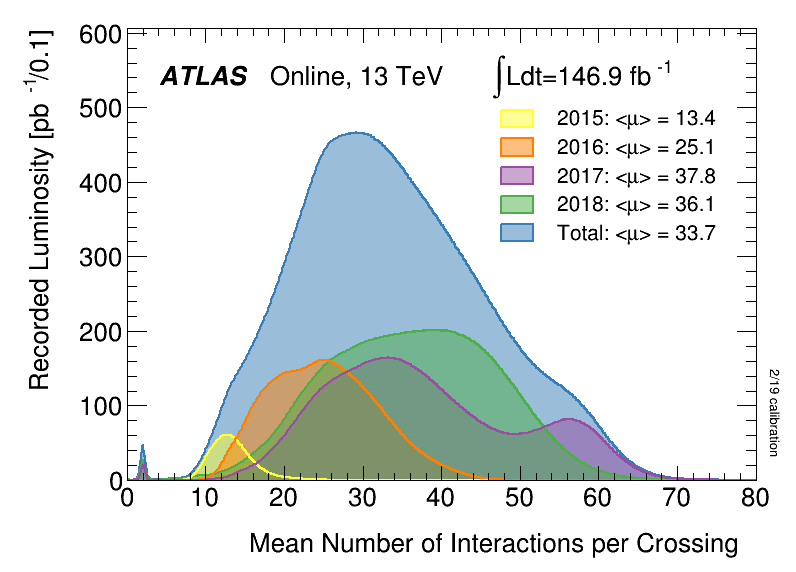
\includegraphics[width=\linewidth]{3_experiment/lhc/PileupConditionsRun2.png}
        \caption{Run-2}
        \label{fig:atlas:runs:pileup_run2}
    \end{subfigure}
    \hfill
    \begin{subfigure}[h]{0.46\linewidth}
        \centering
        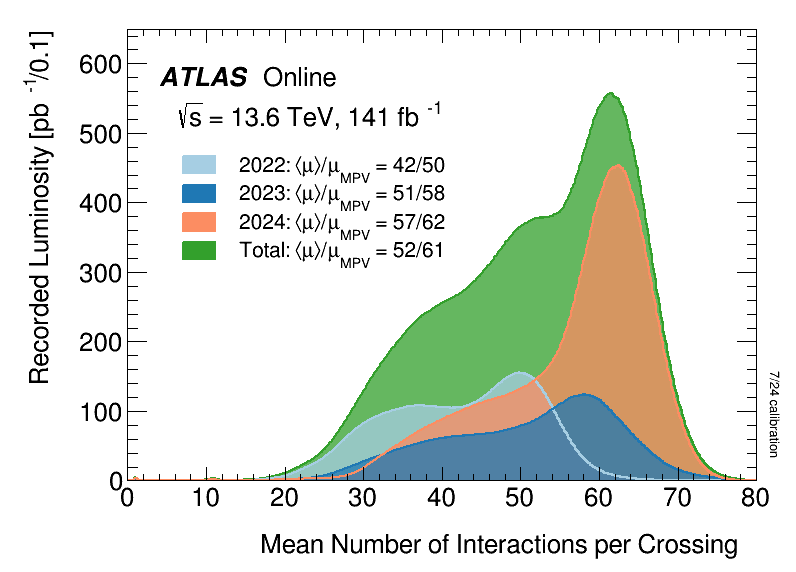
\includegraphics[width=\linewidth]{3_experiment/lhc/PileupConditionsRun3.png}
        \caption{Run-3}
        \label{fig:atlas:runs:pileup_run3}
    \end{subfigure}
    \caption{Distribuci\'on del n\'umero de interacciones por bunch-crossing durante Run-2 (izquierda) y Run-3 (derecha).}
    \label{fig:atlas:runs:pileup}
\end{figure}
\chapter{Reconstrucci\'on e identificaci\'on de objetos f\'isicos}
\label{ch:objects}
\epigraph{\emph{“Champions keep playing until they get it right.”}}{Billie Jean King}


Las partículas (y los productos de sus decaimientos) producidas en cada colisión, interactúan con el detector de una manera particular según su naturaleza. La información recogida por todos los subdetectores descritos en el capítulo anterior permite reconstruir e identificar los objetos físicos presentes en cada suceso aceptado por el sistema de trigger. Existen dos tipos de reconstrucción e identificación. La \textit{online}, se lleva a cabo al mismo tiempo que se producen las colisiones \pp, y la \textit{offline}, realizada después de que los eventos se guarden para su almacenamiento. La reconstrucción se realiza evento por evento, y se lleva a cabo del mismo modo para los eventos recolectados por el detector \ac{ATLAS} y para los eventos simulados con \acf{MC}. A continuación, se da un breve resumen de la reconstrucción offline y la identificación de los objetos utilizados en esta tesis.







\section{Reconstrucci\'on de trazas y v\'ertices}

En un evento con alto pileup, puede haber del orden de 1000 partículas cargadas pasando por el detector \ac{ATLAS}. La información del \ac{ID} (\Sect{\ref{subsec:atlas:atlas:id}}) se utiliza para reconstruir las trayectorias de las partículas cargadas, denominadas \textit{tracks}.

Dado que el \ac{ID} es el detector más cercano al haz y está compuesto por material mínimamente ionizante con una granularidad elevada, este detector desempeña el papel principal en la reconstrucción de trazas. \'Estas, permiten encontrar el momento y la trayectoria de las partículas cargadas, dado que dejan una se\~nal en las diferentes capas del \ac{ID}. Adem\'as, como el campo solenoidal dentro del \ac{ID} es homogéneo, la trayectoria resultante es circular en el plano \(xy\). Cinco parámetros mostrados en la \Fig{\ref{fig:objects:track_vtx:track_parameters}} definen las trazas de las partículas cargadas:
\begin{itemize}
    \item \(q/\pt\): la relación entre la carga y el momento transverso que define la curvatura.
    \item \(d_0\): la distancia de máxima aproximación al vértice primario en el plano-\(xy\) que define el parámetro de impacto transversal.
    \item \(z_0\): el parámetro de impacto longitudinal a lo largo del eje \(z\).
    \item \(\phi_0\): el ángulo azimutal.
    \item \(\theta_0\): el ángulo polar de la dirección de la partícula en el punto más cercano de aproximación~\cite{ATLAS-Tracks-Performance-Run2}.
\end{itemize}

\begin{figure}[ht!]
    \centering
    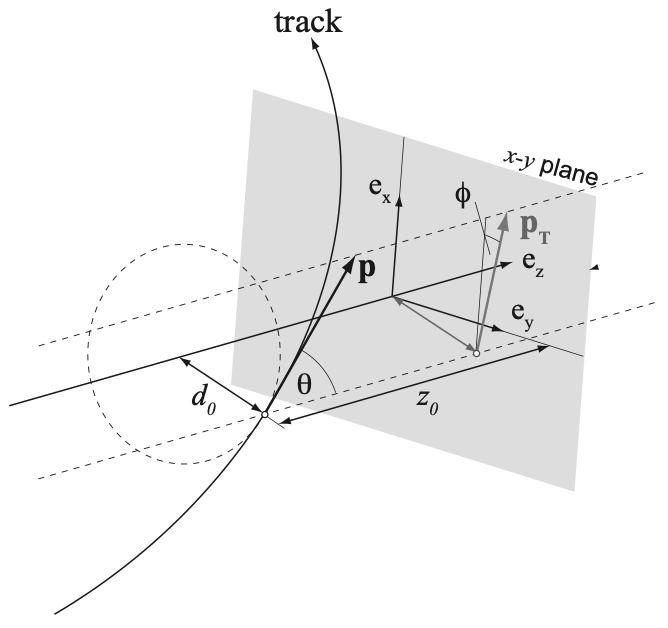
\includegraphics[width=0.6\linewidth]{3_experiment/object_reconstruction/tracking_coordinates.png}
    \caption{Esquema mostrando los par\'ametros usados para la reconstrucc\'on de trazas~\cite{ATLAS-Tracking-2007}.}
    \label{fig:objects:track_vtx:track_parameters}
\end{figure}

La reconstrucción de trazas utilizada en durante el Run-2 utiliza dos enfoques complementarios: el enfoque \textit{inside-out} y el \textit{outside-in}~\cite{ATLAS-NEWT}.

El primer paso para la reconstrucción de trazas en el m\'etodo inside-out es la búsqueda de \textit{seeds}, en la que se buscan tres hits en el detector de silicio para comenzar la reconstrucción de la traza. A partir de estos tres hits y suponiendo un campo magnético uniforme, se obtiene una primera estimación de los parámetros de la traza. A partir de las seeds de la traza, ésta se extrapola a las demás capas del detector de silicio, a partir de las cuales se utiliza un filtro combinatorio de Kalman para estimar los parámetros de la traza. En esta fase del proceso puede haber varias trazas candidatas para cada seed. Una vez formada la traza, se aplica un algoritmo de resolución de ambigüedades para reasignar los clusters compartidos a la traza con mejor coincidencia~\cite{ATLAS-NNClustering}, y se ajusta la traza candidata final utilizando un método global \chisq. La última parte del método inside-out consiste en extender las trazas hasta el \ac{TRT}, e incluir los hits del \ac{TRT}, para mejorar as\'i su resolución del momento.

Para mejorar la eficiencia de las trazas de los decaimientos desplazados del punto de colisión original, se utiliza el m\'etodo \textit{outside-in}. Se utilizan los hits del \ac{TRT} para comenzar la reconstrucci\'on de la traza y luego se extiende para incluir los hits del detector de silicio, aplicándose de nuevo un algoritmo para resolver las ambigüedades, mitigando as\'i los hits compartidos entre m\'ultiples trazas.

Los vértices primarios y secundarios son de vital importancia para la posterior reconstrucción de objetos en \ac{ATLAS}. En este paso, las trazas encontradas como se ha explicado anteriormente se utilizan como \textit{input} para el algoritmo de reconstrucci\'on de vértices~\cite{ATLAS-PVReconstruction,ATLAS-VertexReconstruction}. En primer lugar, el \ac{PV} se define como el lugar donde se da la interacci\'on entre los dos protones inyectados por el \ac{LHC}. Los \acp{PV} se reconstruyen emparejando las trazas que se cruzan, lo que se realiza en tres pasos principales: b\'suqueda de seeds, asignación de trazas y ajustes. Finalmente, el vértice con el mayor \(\sum \pt^2\) para todas las trazas asociadas, que tambi\'en se denomina vértice de dispersión dura, se asigna como el \ac{PV}.
Hay algunas partículas que decaen rápidamente tras su producción, como los leptones \(\tau\) o los quarks más pesados (\(b\) o \(\cquarks\)), y su posición de decaimiento puede medirse. A partir de las trazas restantes originadas por estos decaimientos, es posible identificar vértices secundarios. Todos los vértices reconstruidos restantes se consideran pileup.








\section{Fotones y electrones}

La reconstrucción de electrones y fotones en el \ac{ATLAS} se basa en la deposición de energía en el \ac{ECAL}. Como los electrones y los fotones dejan señales similares en este calor\'imetro, su reconstrucción se realiza simultáneamente, distinguiéndolos por la información de las trazas reconstruidas que se mostr\'o anteriormente.


\subsection{Reconstrucci\'on}
\label{subsec:objects:egamma:reco}

La reconstrucción de fotones y electrones \textit{offline}~\cite{ATLAS-EGamma-Performance-2015-2017,ATLAS-TopoClusters-Run2} hace uso de clusters dinámicos de tamaño variable, conectados topológicamente entre las celdas del \ac{ECAL} y \ac{HCAL}~\cite{ATLAS-TopoClusters-Run1}, denominados \textit{\topos}, que se agrupan adem\'as en \textit{superclusters}. 
Durante el Run-1~\cite{ATLAS-EGamma-Performance-Run1, ATLAS-EGamma-CalibrationPerformance-Run1, ATLAS-CalorimeterClustering-2008}, en contraste, los clusters eran de tama\~no fijo, y que si bien ten\'ian una respuesta lineal energ\'etica y estabilidad frente al pileup, no permit\'ia reconstruir eficientemente la energ\'ia de fotones bremsstrahlung o de electrones/positrones producto de la creaci\'on de pares. La implementaci\'on de superclusters durante el Run-2, junto con la calibraci\'on de la energ\'ia descripta en la \Refn{\cite{ATLAS-EGamma-Calibration-2015-2016}} permite solucionar esto sin perder la linealidad y estabilidad de los clusters de tama\~no fijo.
De esta forma, se distinguen tres tipos de objetos:
\begin{itemize}
    \item Electrones: consiste en un cluster construido a partir de los depósitos de energía en el \ac{ECAL} el cual tiene asignado una traza.
    \item Fotones convertidos: consiste en un cluster asignado con un vértice (o vértices) de conversión.
    \item Fotones no convertidos: un cluster que no se encuentra emparejado ni a una traza ni a un vértice de conversión.
\end{itemize}

\begin{figure}[ht!]
    \centering
    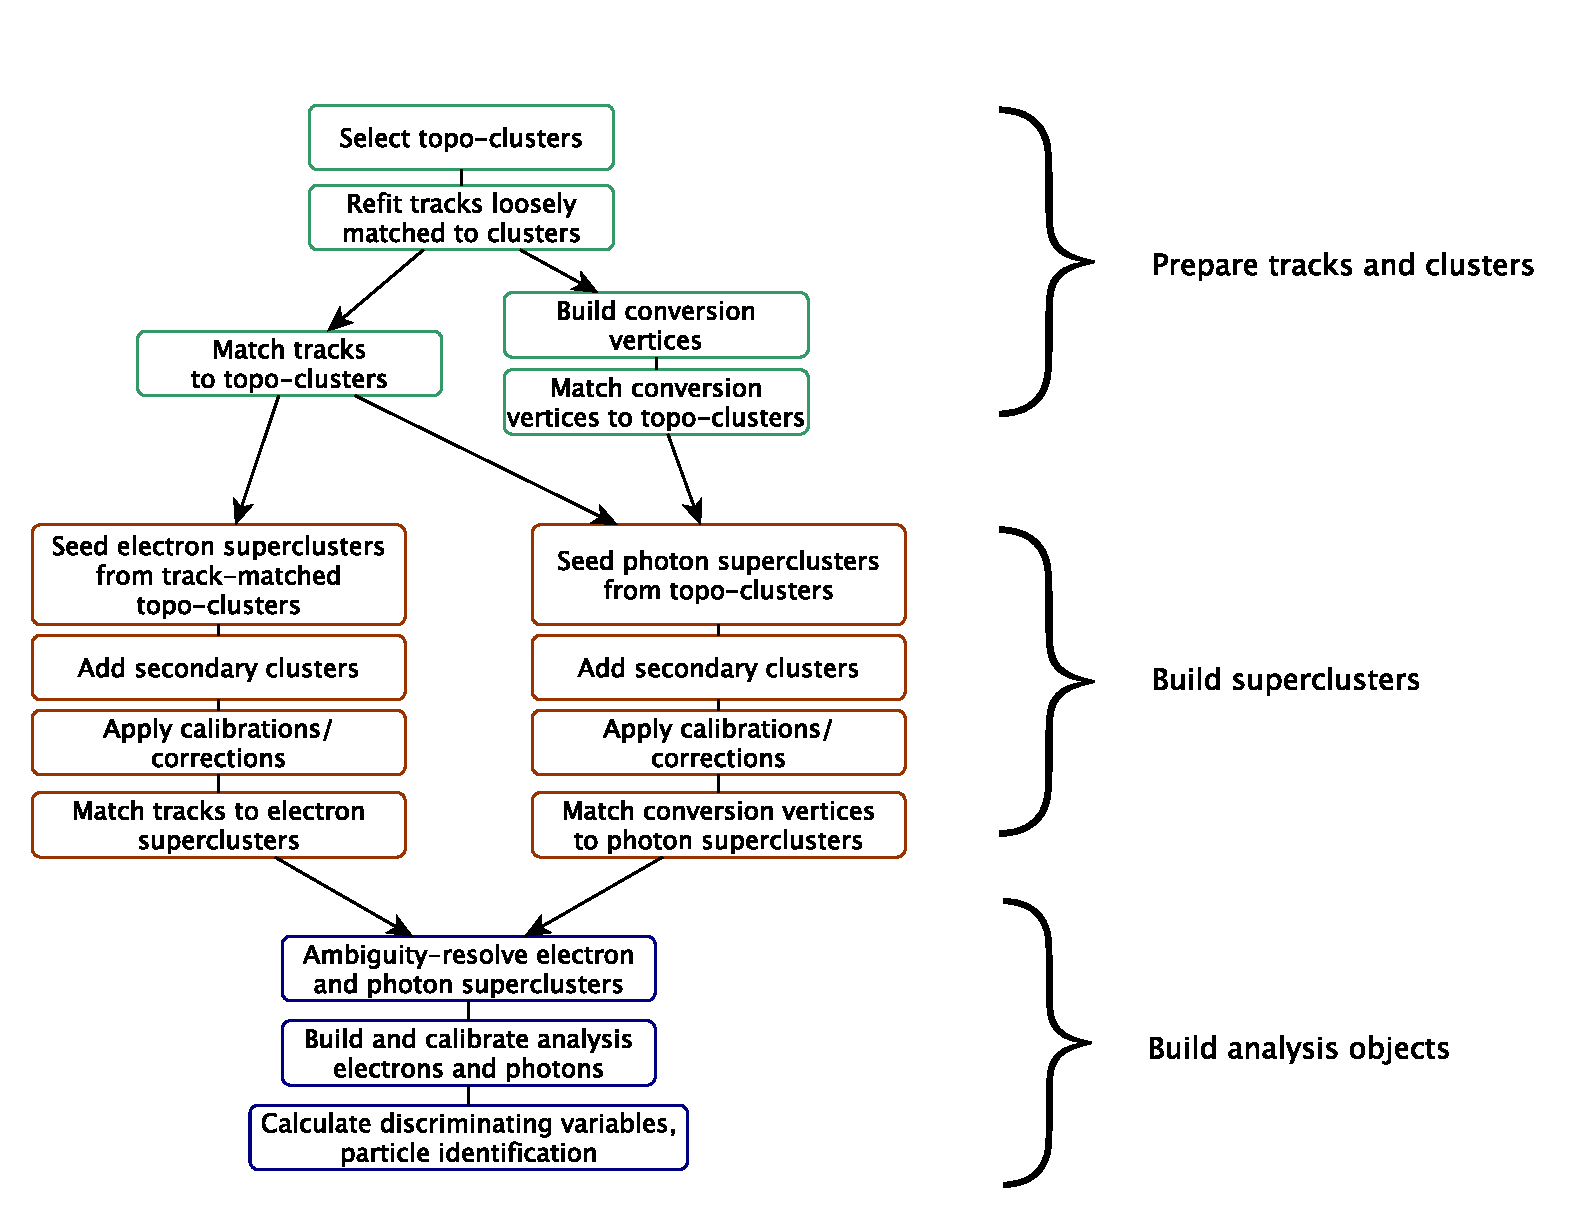
\includegraphics[width=0.8\linewidth]{3_experiment/object_reconstruction/egamma_reconstruction}
    \caption{Diagrama mostrando el algoritmo de reconstrucci\'on de electrones and fotones, extra\'ido de \Refn{\cite{ATLAS-EGamma-Performance-2015-2017}}}
    \label{fig:objects:egamma:reco:reco_diagram}
\end{figure}

El algoritmo para la reconstrucción de electrones y fotones procede como se muestra en la \Fig{\ref{fig:objects:egamma:reco:reco_diagram}}.
El proceso de reconstrucción comienza con la formación de \topos. Primero, se forman proto-clusters en el \ac{ECAL} y \ac{HCAL} agrupando celdas que tienen una requerida y predefinida energía, y añadiendo posteriormente celdas vecinas en cuatro pasos consecutivos, obteniendo as\'i los \topos. Las reconstrucciones contin\'uan sólo en aquellos casos en los que la energía de los \topos en el \ac{ECAL} es superior a \(400~\mev\) y que la fracci\'on de la misma con respecto a la energ\'ia total del \topo sea mayor a \(0.5\), reduciendo gran parte los efectos de pileup.

El algoritmo también construye vértices de conversión a partir de las trazas reajustadas y los empareja con los \topos seleccionados.
Tras el ajuste inicial de las trazas y la construcción de las conversiones, los algoritmos de superclusters de electrones y fotones se ejecutan por separado y en paralelo. En la primera etapa, los \topos se evalúan para su uso como candidatos a clusters semilla, que forman la base de los superclusters; en la segunda etapa, los clusters cercanos a los candidatos a clusters semilla se identifican como candidatos a clusters satélite, que pueden surgir de la radiación bremsstrahlung o de la división de los \topos. Los clusters satélite se añaden a los candidatos a semilla para formar los superclusters finales, si superan unos ciertos criterios de selección necesarios.
Tras aplicar correcciones de posición iniciales a los superclusters resultantes, el algoritmo de reconstrucción hace coincidir las trazas con los superclusters de electrones y los vértices de conversión a los superclusters de fotones.

Dado que un objeto puede reconstruirse como electrón y como fotón, se realiza una resolución de ambigüedad para eliminar parte del solapamiento. Sin embargo, se permite cierto solapamiento para mantener una alta eficiencia de reconstrucción de electrones y fotones, y luego se deja a que los análisis pueden aplicar sus propios criterios. Finalmente, se construyen y calibran los electrones y fotones finales, lo que facilita el cálculo de las variables adicionales utilizadas para los cortes de calidad y la resolución de ambigüedades.



\subsection{Identificaci\'on}
\label{subsec:objects:egamma:id}

Con el objetivo de poder discrminar los objetos \textit{prompt}\footnote{El término \textit{prompt} hace referencia a aquellos objetos producidos rápidamente luego de la colisión, generalmente provenientes del vértice primario, para distinguirlos de aquellos producidos por el decaimiento tardío de otra partícula, como puede ser un hadrón.} de aquellos que no lo son, existen diferentes criterios de identificaci\'on. En \ac{ATLAS}, para fotones y electrones, esto se logra mediante una serie de variables denominadas \acfp{SS}, que con ciertos algoritmos, se logra incrementar la pureza de los objetos deseados, al costo de tener una menor eficiencia de selecci\'on. Finalmente, se definen diferentes \acp{WP} que son derivados de forma central y luego distribu\'idos a toda la colaboraci\'on.

El objetivo principal de la identificaci\'on de electrones es separar los electrones prompt de los electrones producto del proceso de creaci\'on de pares a partir de los fotones, de los jets que depositan energ\'ia en el \ac{ECAL}, y de los electrones proveninentes del decaimiento de hadrones de \textit{heavy-flavor}. La identificaci\'on se basa en un m\'etodo likelihood que utiliza algunas de las variables que ser\'an descriptas en el \Ch{\ref{ch:pid_ss}}, utilizando electrones provenientes de decaimientos de \jpsi y \Zboson para bajo y alto \et, respectivamente~\cite{ATLAS-EGamma-Performance-2024}. Se definen entonces 3 \acp{WP}, denominados \texttt{Loose}, \texttt{Medium} y \texttt{Tight}, cuyas eficiencias de identificaci\'on de un electr\'on con \(\et=40~\gev\) son de \(93\%, \, 88\%\) y \(80\%\), respectivamente~\cite{ATLAS-EGamma-Calibration-2015-2016}.


Para distinguir los fotones reales (los procedentes de la colisión) de los fotones de fondo que tienen secciones transversales de producción mucho mayores (procedentes del decaimiento de hadrones, también llamados fotones falsos), es necesario basarse en un algoritmo de identificación con alta eficiencia de señal y rechazo de fondo, para fotones candidatos con \(\pt \sim 10~\gev\) hasta la escala \tev.
Actualmente, la identificación de fotones en \ac{ATLAS} se basa en un conjunto de cortes rectangulares en las \acp{SS} mencionadas anteriormente, que son calculadas a partir de la energía depositada en las celdas del cluster en la primera y segunda capa del \ac{ECAL}, y de la fuga hacia el \ac{HCAL}. Estas variables describen el paso de los fotones a través de los calorímetros, caracterizando las lluvias electromagnéticas laterales y longitudinales.
El proceso completo de identificación de fotones se presenta en \Ch{\ref{ch:pid_ss}}, donde las \acp{SS} se explican una a una. Además, en los \Chs{\ref{ch:ffs}}{\ref{ch:cellrw}} se presentan dos enfoques para corregir las diferencias observadas en estas variables entre los datos y \ac{MC}.





\subsection{Aislamiento}
\label{subsec:objects:egamma:iso}

Para mejorar aún más la selecci\'on de fotones y electrones se aplican criterios de aislamiento a estos objetos. A su vez, la presencia de otros objetos cerca del fotón o el electrón puede interferir en la correcta reconstrucción de las variables cinemáticas del mismo, como su energía. Para ello, se definen dos criterios de aislamiento: calorim\'etrico y de trazas. 

\begin{figure}[ht!]
    \centering
    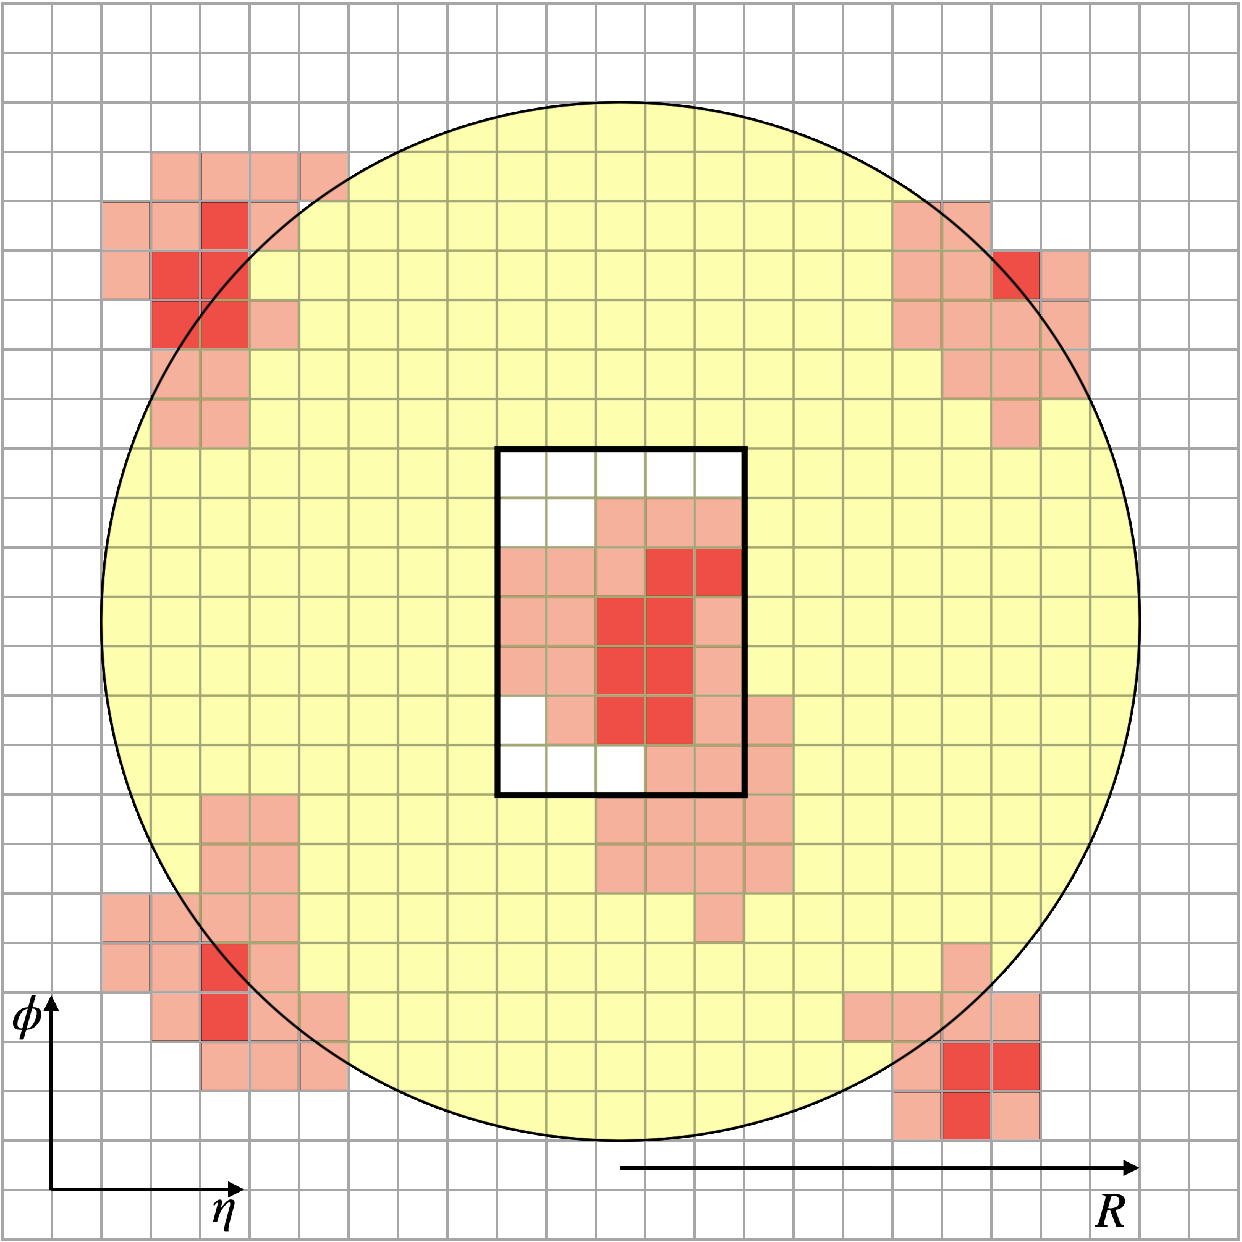
\includegraphics[width=0.5\linewidth]{3_experiment/object_reconstruction/isolation_diagram}
    \caption{Diagrama mostrando el proceso del c\'alculo de la variable de aislamiento calorim\'etrico. Cuando se utiliza un cono con \(R=0.4\), se puede construir la variable \etconefo mencionada en el texto.}
    \label{fig:objects:egamma:iso:iso_diagram}
\end{figure}

El procedimiento para calcular la energía de aislamiento calorim\'etrico \etconefo es el siguiente, y se muestra en la \Fig{\ref{fig:objects:egamma:iso:iso_diagram}}. En primer lugar, se construye un cono de radio \(\DeltaR<0.4\) alrededor del candidato a fotón o electrón, y se suman las energías de todas las celdas de los \topos (introducidos en la \Sect{\ref{subsec:objects:egamma:reco}}) cuyos baricentros se encuentran dentro del cono. A continuación, a esta energía calculada, se le resta la energía de todas las celdas en una ventana de \(5\times 7\) (en unidades de \(\eta \times \phi\) en la segunda capa del \ac{ECAL}) centrada alrededor del candidato, con el fin de eliminar la energía del propio candidato. También se tienen en cuenta las contribuciones del pileup y las fugas de energía fuera del cono.

La variable de aislamiento de trazas, \ptconetw, se obtiene sumando los \pt de las trazas de buena calidad en un cono de radio \(\DeltaR<0.2\) alrededor del candidato a electrón o en la dirección del cluster de fotones convertidos.
Se excluyen de este cómputo las trazas asociadas a la traza o al fotón convertido, así como aquellas trazas que no pasan el requisito de trazas de buena calidad. Una traza de buena calidad se define como aquella en la que el \pt es \(\pt>1~\gev\), y tiene una distancia mínima al vértice primario a lo largo del eje \(z\) de \(|z_0 \sin \theta| < 3\) mm.

En general, para los fotones y electrones, no hay otra energía depositada en el cono alrededor del candidato, aparte de los objetos de baja energía originados por los restos de la colisión, las interacciones múltiples y el pileup. En cambio, para los falsos candidatos a fotones y los fotones no directos, se observa energía adicional dentro del cono, originada por los objetos que acompañan al jet.

\begin{table}[ht!]
    \caption{Resumen de los \ac{WP} de aislamiento para electrones y fotones usados a lo largo de esta tesis.}
    \resizebox{\linewidth}{!}{
        \begin{tabular}{|l|c|c|c|}
            \hline
            Objecto                      & \ac{WP}                             & Aislamiento Calorim\'etrico                                    & Aislamiento de trazas   \\ \hline
            \multirow{3}{*}{Fot\'on}     & \texttt{FixedCutLoose}         & \(E_{T}^{\text{cone20}}<0.065\times \pt \)                & -                                  \\
                                        & \texttt{FixedCutTightCaloOnly} & \(\etconefo < 0.022\times \pt + 2.45~\gev\)               & -                                  \\
                                        & \texttt{FixedCutTight}         & \(\etconefo < 0.022\times \pt + 2.45~\gev\)               & \(\ptconetw/\pt < 0.05\)           \\ \hline
            \multirow{2}{*}{Electr\'on}   & \texttt{Loose\_VarRad}         & \(\etconetw < 0.2\times\pt\)                              & \(\pt^{\text{cone30}}/\pt < 0.15\) \\
                                        & \texttt{HighPtCaloOnly}        & \(\etconetw < \max\left(0.015\times\pt, 3.5~\gev\right)\) & -                                  \\ \hline
        \end{tabular}
    }
    \label{fig:objects:egamma:iso:iso_table}
\end{table}

A partir del aislamiento calorimétrico y de trazas se pueden definir diferentes \acp{WP} por separado tanto para electrones como para fotones. En el caso de los electrones, se definen dos estrategias: o bien conseguir una eficiencia fija, o bien aplicar cortes fijos en las variables de aislamiento. En el caso de los fotones, hay \acp{WP} que no utilizan ambas variables de aislamiento, como es el caso del \ac{WP} que sólo utiliza el aislamiento calorimétrico. Las definiciones de los diferentes \acp{WP} utilizados a lo largo de esta tesis se muestran en la \Tab{\ref{fig:objects:egamma:iso:iso_table}}. Además, es común definir las siguientes variables para \ac{WP} \texttt{FixedCutTight} del fotón:
\begin{align}
    \etiso &= \etconefo - 0.022 \times \et - 2.45~\gev\\
    \ptiso &= \ptconetw / \et
\end{align}
dejando por tanto las variables definiendo el \ac{WP} \texttt{FixedCutTight} como:
\begin{align}
    \etiso &< 0 ~\gev\\
    \ptiso &< 0.05.
\end{align}















\section{Muones}



La tasa de radiación bremsstrahlung es inversamente proporcional al cuadrado de la masa de una partícula. Dado que los muones son unas 200 veces más pesados que los electrones, interactúan principalmente con el material del detector a través de ionización. Por lo tanto, los muones son partículas mínimamente ionizantes que no crean lluvia electromagnética en los calorímetros y atraviesan todas las capas del detector \ac{ATLAS}. Es por esta raz\'on que la detección de muones depende de las mediciones de las trazas dejadas por ellos en el \ac{ID} y el \ac{MS}. La combinación de los dos subdetectores define cuatro tipos de muones, dependiendo de la información utilizada para la reconstrucción:
\begin{itemize}
    \item \ac{CB}: mu\'on reconstruido a partir de un reajuste global de las trazas del \ac{ID} y del \ac{MS},
    \item \ac{ST}: mu\'on reconstruido a partir de una traza ajustada del \ac{ID} que al extrpolarla al \ac{MS} tienen un segmento en el \ac{MDT} o el \ac{CSC},
    \item \ac{CT}: mu\'on reconstruidos a partir de la traza del \ac{ID} ajustada a los depósitos de mínima energía ionizante en los calorímetros,
    \item \ac{ME}: mu\'on reconstruido únicamente a partir de las trazas \ac{MS}.
\end{itemize}

El solapamiento entre distintos tipos de muones se resuelve del siguiente modo. Cuando dos tipos de muones comparten la misma traza del \ac{ID}, el orden de preferencia es: primero el \ac{CB}, luego el \ac{ST} y finalmente el \ac{CT}. El solapamiento con \ac{ME} se resuelve analizando los hits de las trazas, seleccionando aquellas trazas con mejor ajuste y mayor número de hits.

Para la identificación de muones, se aplican cortes de calidad para distinguir los muones aislados de los procedentes de procesos de fondo, principalmente del decaimiento de piones y kaones.
Las variables con buen poder discriminatorio utilizadas se describen en \Refn{\cite{ATLAS-Muon-Performance-2016}}. Se definen cuatro selecciones de identificación: \texttt{Loose}, \texttt{Medium}, \texttt{Tight} y \texttt{High-pT}. Las tres primeras categorías son inclusivas, siendo \texttt{Medium} la selección por defecto en \ac{ATLAS}. Por último, se pide a los candidatos a muones que van a ser utilizados por los análisis que satisfagan los requisitos de aislamiento, tanto a nivel de trazas como calorimétricos, de forma análoga a los detallados para los electrones y fotones en el apartado anterior. Para el aislamiento de trazas, se utiliza una variable similar a la empleada para los electrones fotones, pero con un cono de radio variable \(\DeltaR = \min(10~\gev/\pt, 0.3)\) alrededor del momento del muón, excluyendo la traza del mismo. Para el aislamiento calorimétrico se utiliza la misma variable \etconefo, con la diferencia de utilizar un radio de \(R=0.2\), en lugar de \(0.4\). En base a estas variables, se definen 7 criterios de selección de aislamiento (7 \acp{WP}), optimizados para diferentes análisis.








\section{Jets}


Debido al confinamiento de color, un quark o gluón no puede existir por sí mismo y pasa por el proceso de hadronización para formar un chorro colimado de partículas de color neutro, denominados \textit{jets}. Generalmente, los jets penetran a través del \ac{ECAL} y son totalmente absorbidos por el material del calorímetro hadrónico. A continuación, se describe brevemente el método típico de agrupación adoptado por \ac{ATLAS}. También se describen los dos tipos existentes de reconstrucción de jets.


\subsection{Algoritmo de clusterizaci\'on de jets \antikt}

Dado que los jets están constituidos por un elevado número de partículas que dejan deposiciones de energía en el \ac{ECAL} y \ac{HCAL} y trazas en el \ac{ID}, un algoritmo de clusterizaci\'on agrupa los constituyentes en el evento para definir los jets. Dicho algoritmo se denomina algoritmo \antikt~\cite{AntiKtAlgorithm}. Del mismo modo que para los electrones y los fotones, la reconstrucción de los jets \ac{ATLAS} se basa en la formación de \topos: depósitos de energía agrupados en las celdas de los calorímetros mediante un algoritmo de combinación secuencial. Entonces, el algoritmo \antikt combina el \topos con los siguientes pasos:
\begin{itemize}
    \item Medir la distancia entre todos los \topos entre sí, y de cada \topo con el haz:
        \begin{gather}
            \dij = \min \left( p_{T,i}^{-2}, p_{T,j}^{-2} \right) \frac{\Delta_{i,j}^2}{R^2}\\
            d_{iB} = p_{T,i}^{-2}
        \end{gather}
        donde \(\Delta_{ij}^2 = \Delta\phi_{ij}^2 + \Delta\eta_{ij}^2\) y \(R\) es el radio del jet.
    \item Si el mínimo de todas las distancias calculadas anteriormente es \(d_{iB}\), el \topo \(i\) se clasifica como jet, y se descarta en iteraciones sucesivas.
    \item Si el mínimo de todas las distancias es \(d_{ij}\), \topos \(i\) y \(j\) se combinan, todas las distancias se calculan de nuevo con este nuevo \topo y la iteración se realiza de nuevo.
\end{itemize}
Este proceso se repite hasta que todas las partículas del evento se han agrupado.

El algoritmo \antikt comienza agrupando la radiación alrededor de la partícula más dura del evento, ya que la partícula con mayor \pt definirá el término \(\min \left( \frac{1}{p_{T,i}^2}, \frac{1}{p_{T,j}^2}  \right)\) en la definición de \dij. Esto permite que los jets del evento tengan una dirección estable al principio del proceso de combinación. El algoritmo \antikt es preferible a otros algoritmos secuenciales de jets ya que los jets tienen formas regulares que son aproximadamente cónicas, mostrados en la \Fig{\ref{fig:objects:jets:antikt}}. Los jets que se originan a partir de quarks o gluones en general se denominan small-\(R\) jets y para su reconstrucción se utiliza un radio de \(R=0.4\). Por otro lado, los jets que representan partículas masivas que decaen hadrónicamente se denominan large-\(R\) jets, y se utiliza \(R=1.0\), dado que el uso de un cono más amplio ayuda a incluir la mayoría de las partículas producto del decaimiento.


\begin{figure}[ht!]
    \centering
    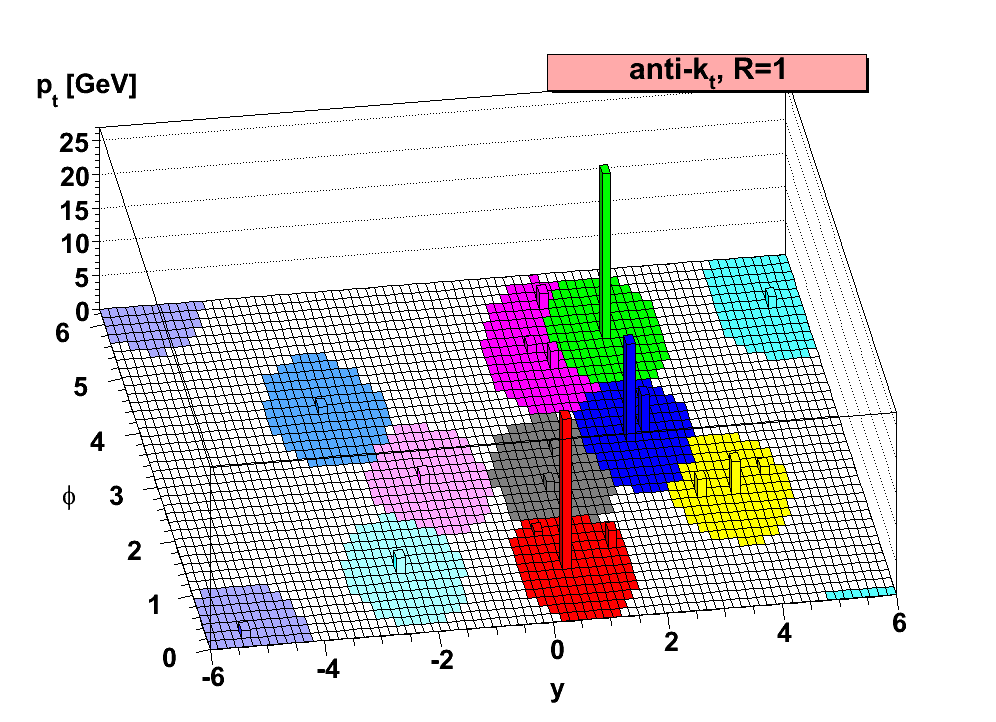
\includegraphics[width=0.7\linewidth]{3_experiment/object_reconstruction/antikt_clusters}
    \caption{Representaci\'on esquem\'atica del algoritmo \antikt para el proceso de clusterizaci\'on de jets~\cite{AntiKtAlgorithm}.}
    \label{fig:objects:jets:antikt}
\end{figure}

\subsection{Jets Calorim\'etricos}

Una forma de reconstruir los jets se basa en los depósitos de energía en el calorímetro. De forma similar a lo que se ha explicado para electrones y fotones en \Sect{\ref{subsec:objects:egamma:reco}}, los depósitos de energía en las celdas del \ac{ECAL} y \ac{HCAL} se utilizan para construir \topos, que aproxima los depósitos de energía de hadrones individuales~\cite{ATLAS-TopoClusters-Run1,ATLAS-TopoClusters-Run2}. Los jets reconstruidos de esta manera y agrupados con el algoritmo \antikt con un radio de \(R=0.4\) se denominan jets \textsc{EMTopo}, y son los proxies de los quarks y gluones individuales. En la reconstrucción de jets, sólo se incluyen los \topos con energía neta positiva.

\subsection{\acf{PFlow} Jets}

Otro m\'etodo para la reconstrucci\'on de jets se basa en el algoritmo \ac{PFlow}~\cite{ATLAS-JetPFlow-Performance}, en el que las mediciones del \ac{ID} y del calorímetro se combinan para formar las señales, que idealmente representan partículas individuales. El algoritmo comienza vinculando cada traza del \ac{ID} con un solo \topo. Luego se calcula la energ\'ia esperada en el calor\'imetro depositada por cada part\'icula que tambi\'en inici\'o la traza. Luego, para cada sistema \topo/traza, el algoritmo eval\'ua la probabilidad de que la energ\'ia de la part\'icula haya sido depositada en m\'as de un \topo, y decide si es necesario agregar m\'as \topos al sistema \topo/traza para recuperar la energ\'ia total del la lluvia. Posteriormente, la energ\'ia depositada por la part\'icula que inicia la traza es sustra\'ida celda por celda del conjunto de \topos vinculados. Finalmente, si la energ\'ia remanente en el sistema es consitente con la esperada por las fluctuaciones de la lluvia de la se\~nal de una sola part\'icula, los remanentes del \topo son removidos.

El resultado de este algoritmo es un conjunto de trazas, y un conjunto de \topos modificadas y no modificadas por el procedimiento anterior, que son los objetos \ac{PFlow}. Los objetos \ac{PFlow} también pueden agruparse con el algoritmo \antikt y el mismo \(R=0.4\) para formar los jets \ac{PFlow}.

El algoritmo \ac{PFlow} tiene bastantes ventajas sobre el \textsc{EMTopo}:
\begin{itemize}
    \item La resolución en \pt del \ac{ID} es significativamente mejor que la resolución de energía del calorímetro para partículas cargadas de baja energía.
    \item Permite una mayor aceptancia para partículas más \textit{soft}. Las trazas se reconstruyen para partículas cargadas con un mínimo \pt de \(400~\mev\), el cual es menor que el requerido para la formaci\'on de \topos.
    \item Mejora la resolución angular de una sola partícula cargada, ya que utiliza la información del \textit{tracker} (\acf{ID}) en lugar de la del calorímetro.
    \item Las partículas cargadas de bajo \pt que se originan dentro de un jet hadrónico son barridas fuera del cono del jet por el campo magnético para cuando alcanzan el calorímetro. Utilizando la coordenada azimutal de las trazas en el perigeo, estas partículas tambi\'en son agrupadas en el jet.
    \item Es posible eliminar las trazas originadas por el pileup, sabiendo que éstas no proceden del \ac{PV}.
\end{itemize}

Sin embargo, tambi\'en introduce una complicación. Para cualquier partícula cuya medición de traza deba utilizarse, es necesario identificar correctamente y sustraer su señal en el calorímetro para evitar un doble conteo. En el algoritmo \ac{PFlow}, se toma una decisión booleana sobre si utilizar la medición del tracker o del calorímetro. La capacidad de sustraer con precisión toda la energía de una sola partícula, sin eliminar la energía depositada por otras partículas, constituye el criterio clave de rendimiento sobre el que se optimiza el algoritmo.

En esta tesis, se consideran los \ac{PFlow} jets, ya que han demostrado proporcionar una mejor reconstrucción del jet~\cite{ATLAS-JetPFlow-Performance}, principalmente para aquellos con bajo \pt y en la reconstrucción \met~\cite{ATLAS-MET-Performance-2016}.


\subsection{Calibraci\'on de jets}

Una vez reconstruidos los jets, su cuadrimomento se corrige para que coincida con la cinemática de un \textit{truth}-jet\footnote{Los truth jets, o jets reales, provienen de part\'iculas del estado final de simulaciones, luego de pasar por el algoritmo de clusterizaci\'on \antikt.}, como se muestra en la \Fig{\ref{fig:objects:jets:jet_calib:jet_calib_sequence}}. Las tres primeras correcciones tienen en cuenta la contaminación de la distribución de pileup subyacente y las fluctuaciones debidas al origen del jet~\cite{ATLAS-Jet-Calibration-Run2}. La \textit{Global Sequential Calibration} mejora la resolución de \pt de los jets (y las incertidumbres asociadas) eliminando secuencialmente la dependencia de la respuesta reconstruida del jet (\(R= E^{\text{reco}} / E^{\text{truth}}\)) en diversos observables. Por último, las diferencias residuales entre los datos y \ac{MC} se tienen en cuenta midiendo el desequilibrio de momento en \Zjets, \gammajet y eventos multijet.

\begin{figure}[ht!]
    \centering
    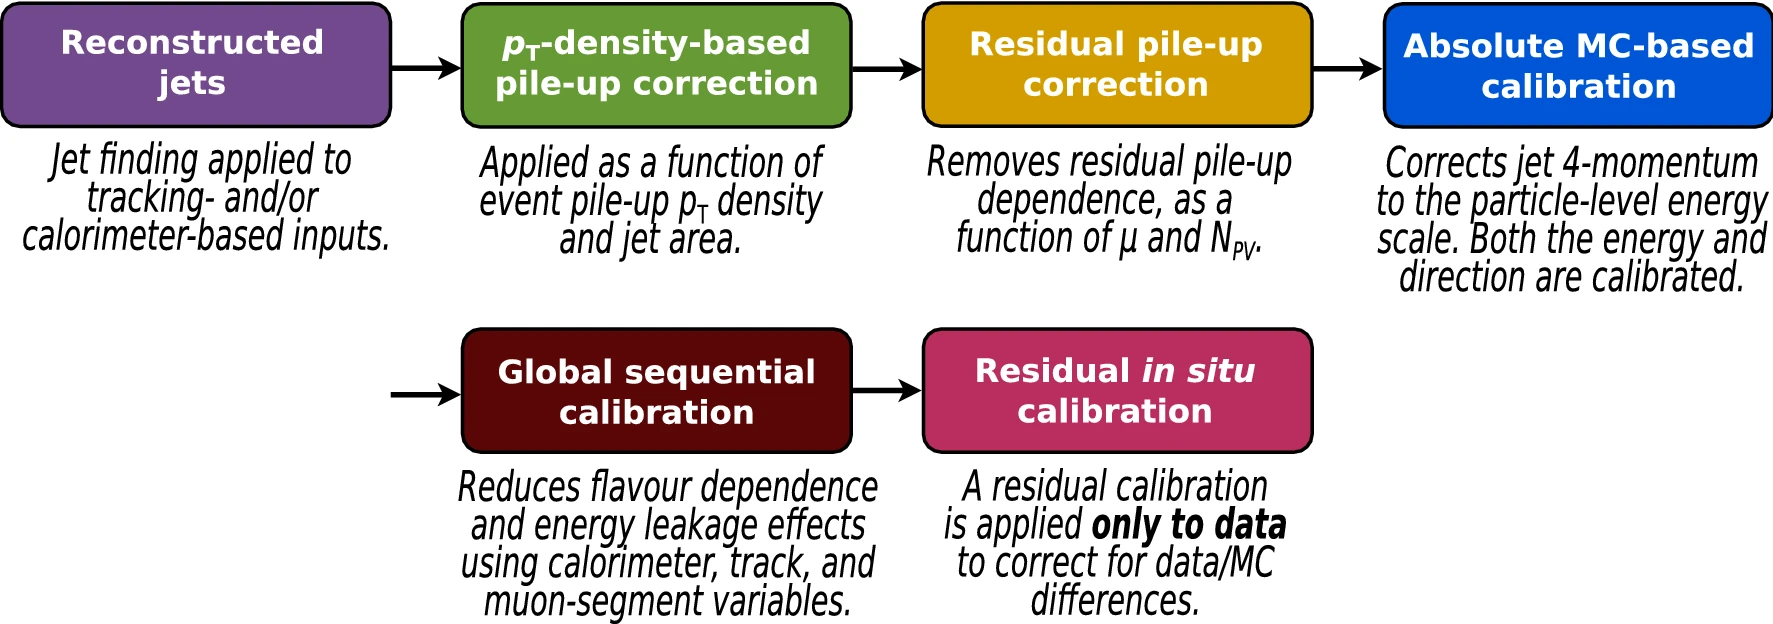
\includegraphics[width=\linewidth]{3_experiment/object_reconstruction/jet_calibration}
    \caption{Pasos para la calibraci\'on del cuadrimomento de \texttt{PFLow} jets~\cite{ATLAS-Jet-Calibration-Run2}.}
    \label{fig:objects:jets:jet_calib:jet_calib_sequence}
\end{figure}

Para reducir el número de jets con una fracción considerable de energía procedente del pileup, se utiliza el algoritmo \ac{JVT}. Este algoritmo \fixme{update to NNJVT} reconstruye un discriminante multivariante que combina, entre otras cantidades, el \ac{JVF} (fracción de las trazas \pt asociada a un jet originado por el \ac{PV}, y el número total de trazas) y el número de \acp{PV} en el evento \Npv. Como los jets que no proceden de la interacción hard-scatter son generalmente más suaves, el corte \ac{JVT} se aplica sólo a los jets con \(\pt<60~\gev\) y \(\abseta<2.4\). El \ac{JVT} \ac{WP} por defecto es \(96\%\) eficiente para los jets de dispersión dura.


















\section{Jets de sabor pesado (\textit{heavy flavor})}

Las decaimientos de hadrones pesados (de ahora en m\'as heavy-flavor) se rigen principalmente por el hadrón más pesado en la cascada de decaimiento. Un hadrón \(b\) generalmente decae en cascada a un hadrón \(c\), que a su vez decae a un hadrón \(s\), etc., lo que conduce a la existencia de múltiples vértices.

\ac{FTAG} es la clasificación de los jets que contienen hadrones \(b\) (\bjets), \(c\) (\cjets) o ni \(b\) ni \(c\) (jets livianos, o \ljets) utilizando algoritmos sensibles a las propiedades distintivas de las respectivas clases.
Estos complejos algoritmos se basan en los múltiples vértices, en la elevada masa, la alta multiplicidad de decaimientos y los modos de decaimiento característicos de los hadrones \(b\) y \(c\), así como en las propiedades de la fragmentación de los quarks pesados.


En \ac{ATLAS} se emplea un proceso de dos etapas para reconstruir las características clave de los heavy-flavor jets. En la primera etapa, los algoritmos de bajo nivel utilizan métodos complementarios para extraer información sobre las trazas de las partículas cargadas vinculadas al jet. Algunos algoritmos se centran en las propiedades de las trazas individuales, mientras que otros analizan sus correlaciones o las combinan para reconstruir explícitamente los vértices desplazados. En la segunda etapa, las salidas de estos algoritmos se integran en un algoritmo de alto nivel que utiliza clasificadores multivariantes para optimizar el rendimiento. Con el tiempo, los algoritmos han evolucionado significativamente, empezando con discriminantes basados en likelihoods y \acp{BDT} durante el Run-1 del \ac{LHC}, y avanzando hacia métodos más avanzados como las redes neuronales recurrentes y profundas, lo que ha dado lugar a notables mejoras en el rendimiento de la identificación~\cite{ATLAS-FTAG-Calibration-2012,ATLAS-FTAG-Efficiency-2012,MV2Algorithm,ATLAS-FTAG-DeepLearning}.

A partir del Run-3, el grupo de \ac{ATLAS} \ac{FTAG}, desarrolla un novedoso algoritmo "GN2" basado en un \textit{Transformer}. El algoritmo GN2 es un único modelo entrenado que sustituye a DL1d~\cite{ATLAS-FTAG-DL1-Run2} y a los algoritmos de bajo nivel que lo alimentan. Se basa en GN1~\cite{ATLAS-FTAG-GN1}, que se refinó rápidamente para pasar a ser GN2. GN2 sustituye la \textit{Graph Attention Network}~\cite{GANs} utilizada por GN1 por un Transformador~\cite{GN2Transformer}, y también se beneficia de otras optimizaciones de arquitectura y de un orden de magnitud más de estadística para su entrenamiento.

GN2 acepta directamente información sobre el jet y las trazas asociadas y, como tal, no depende de otros algoritmos de etiquetado de sabores (\textit{flavor tagging}). GN2 mantiene los dos objetivos de entrenamiento auxiliares que se introdujeron con GN1: la agrupación de trazas que se originan en un vértice común y la predicción del proceso físico subyacente del que se originó cada traza.

Este nuevo algoritmo también está preparado para proporcionar la identificación de \cjets y jets procedentes de decaimientos \(\tau\). Las salidas de este tagger corresponden a las probabilidades de que un jet sea taggeado como un jet \(b\), \(c\), \(\tau\) o \textit{light}, denominadas como \(p_b\), \(p_c\), \(p_{\tau}\) y \(p_u\), respectivamente.

\subsection{Identificaci\'on y performance de \btagging}

Para evaluar la capacidad del tagger de identificar \bjets con una eficiencia constante, se mide la capacidad de rechazar los jets \(c\), \(\tau\) y light. Las probabilidades de salida del tagger se combinan para construir un único discriminante \gntb, definido como
\begin{equation}
    \gntb = \log \left(
        \frac{p_b}{f_c p_c + f_{\tau} p_{\tau} + \left(1-f_c-f_{\tau}p_u\right)}
    \right).
\end{equation}
Los parámetros \(f_{c(\tau)}\) son libres y determinan la importancia entre \(p_{c(\tau)}\) y \(p_u\) en el discriminante. Los valores específicos de estos parámetros se determinan mediante un procedimiento de optimización basado en maximizar el rechazo de \cjets (\(\tau\)-jets) y \ljets, y resultan ser \(0.2\) (\(0.01\)).


A partir de la valor discriminante del tagger, se pueden definir varios \acp{WP}, simplemente exigiendo que el valor \gntb esté por encima de un determinado umbral. El grupo \ac{FTAG} de \ac{ATLAS} proporciona de forma centralizada a toda la colaboración 5 \acp{WP} diferentes para lograr una eficiencia global fija de \btagging: \(65, 70, 77, 85\) y \(90\%\), y se muestran en la \Fig{\ref{fig:objects:jet_tagging:btag_discrminant}}. En dicha figura se comparan tambi\'en las distribuciones de datos y \ac{MC} del tagger GN2, donde las contribuciones de los distintos sabores se muestran con colores diferentes.

\begin{figure}[ht!]
    \centering
    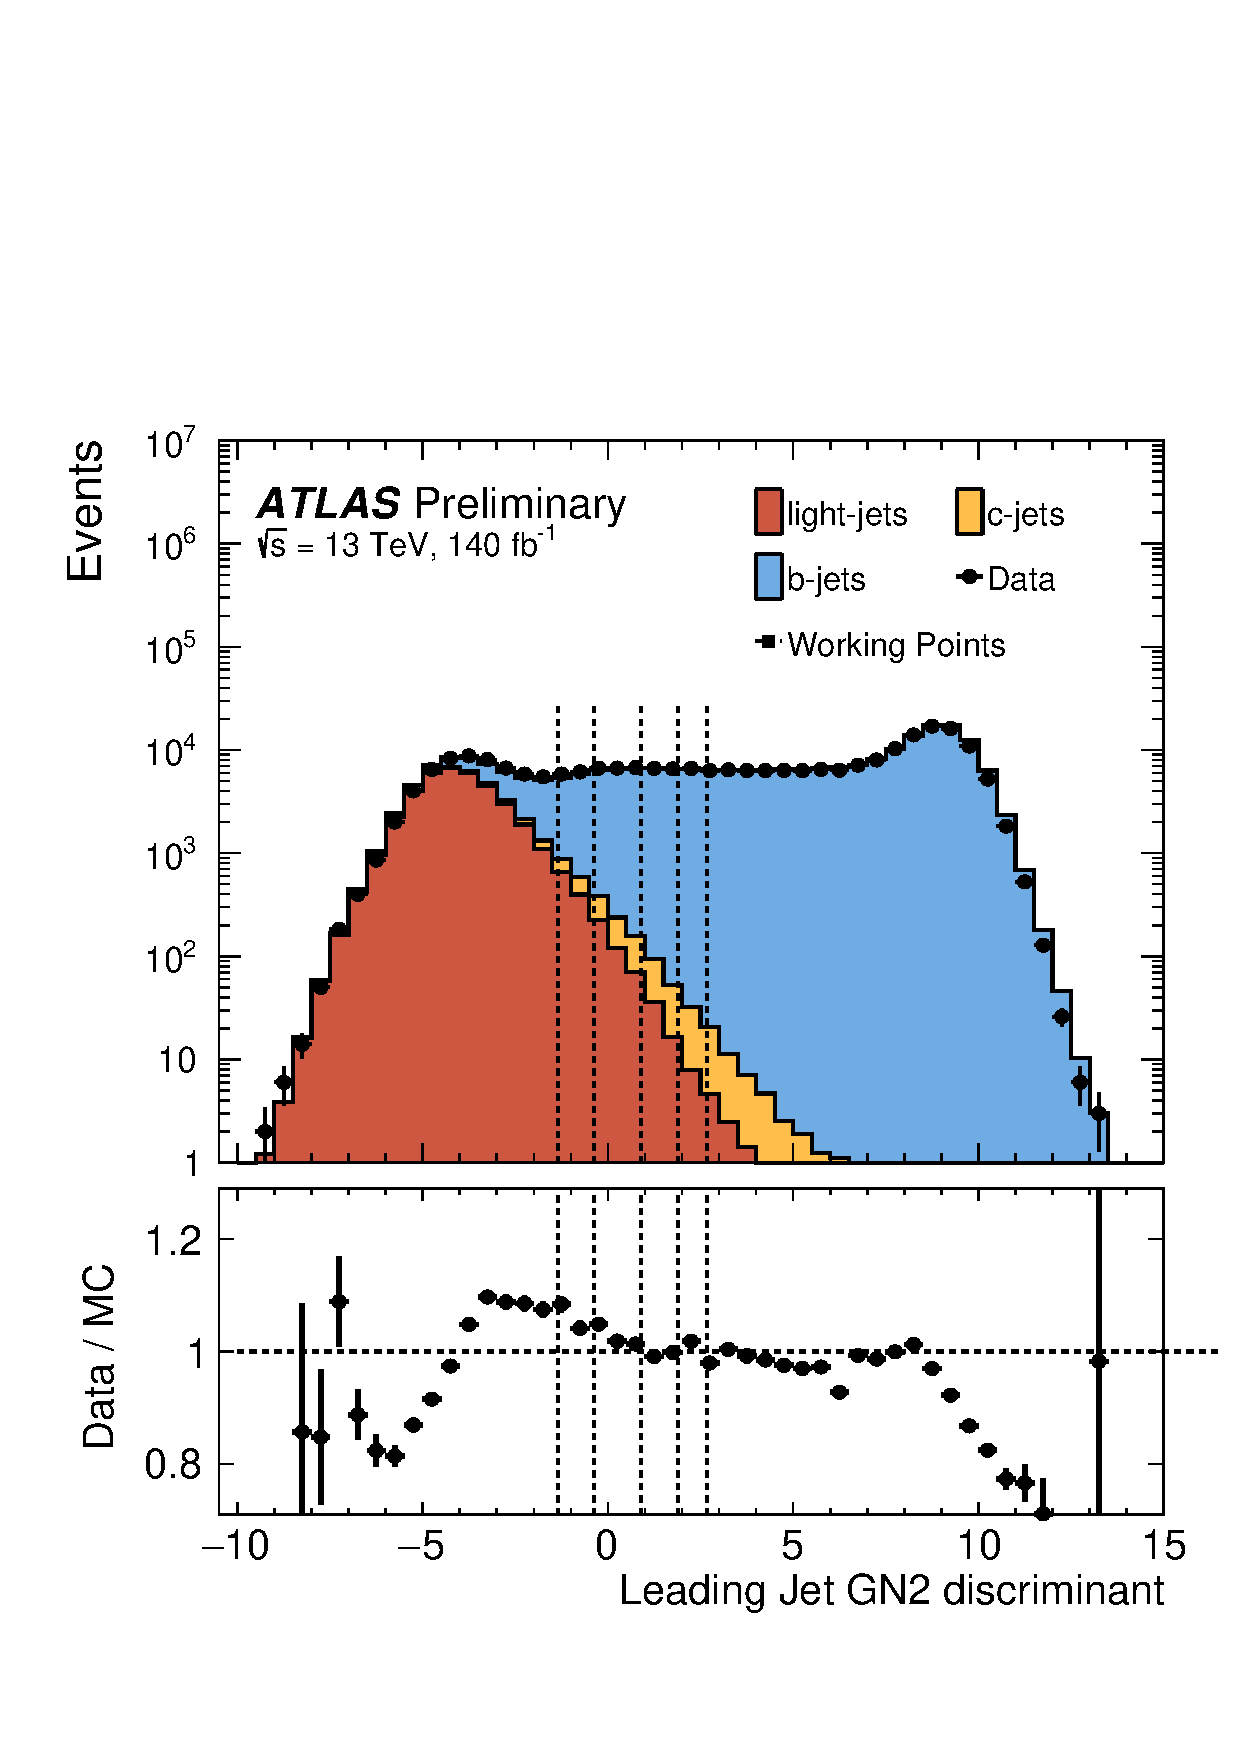
\includegraphics[width=0.6\linewidth]{3_experiment/object_reconstruction/btagging_discriminant}
    \caption{Comparaci\'on entre datos y simulaci\'on \ac{MC} (eventos de \ttbar de un s\'olo lepton) del discriminante del tagger GN2. Las contribuciones de los jets \(l\), \(b\) y \(c\) se muestran con diferentes colores, y los 5 \acp{WP} de \btagging se muestran con las l\'ineas verticales punteadas. De izquierda a derecha, las l\'ineas representan los \acp{WP} de \(90, 85, 77, 70\) y \(65\%\) de eficiencia. El panel inferior muestra el ratio entre los datos y toda la simulaci\'on \ac{MC}~\cite{ATLAS-FTAG-GN2BtagWPs}.}
    \label{fig:objects:jet_tagging:btag_discrminant}
\end{figure}

Uno de los principales problemas del \btagging es la disminución de la eficiencia a mayor \pt. En este régimen de \pt elevado, las partículas son m\'as colimadas y tienden a viajar más lejos en el \ac{ID} antes de decaer, lo que puede dar lugar a una traza de decaimiento con hits espurios. La degradación de la eficiencia se visualiza en la \Tab{\ref{tab:objects:ftag:btag_efficiency_original}}, donde se muestran las eficiencias de tagging para \bjets, junto con los rechazos \cjets, \ljets y \tjets, en los regímenes de bajo y alto \pt. Los valores mostrados se calculan utilizando diferentes muestras, en las que \ttbar se utiliza en la región bajo de \pt y eventos de decaimiento de \(Z'\)~\footnote{El model leptof\'obico de vector axial \(Z'\) es un modelo de Materia Oscura simplificado en el cual el decaimiento teorizado es un par de quarks.} se utilizan en la región alto de \pt. Puede verse que la eficiencia de \btag cae en un \(30\%\) para jets de \pt más alto.

\begin{table}[ht!]
    \caption{Medidas de eficiencias de \btagging, y de rechazos de \cjets, \ljets y \tjets, en los regímenes de bajo y alto \pt.}
    \label{tab:objects:ftag:btag_efficiency_original}
    \resizebox{\textwidth}{!}{
        \begin{tabular}{llcccc}
            \toprule
            Muestra & Rango de \pt [\gev]                                    & Eficiencia de \bjet & Rechazo de \cjet & Rechazo de \ljet & Rechazo de \tjet \\ \midrule
            $t\bar{t}$  & \(20<\pt<250\)    & $0.76$         & $17.52$       & $448.61$               & $71.15$          \\
            $Z'$        & \(250<\pt<6000\)  & $0.41$         & $20.27$       & $179.99$               & $452.94$         \\ \bottomrule
        \end{tabular}
    }
\end{table}

\subsection{Identificaci\'on y performance de \ctagging}

Al igual que con \btagging, se puede construir un único discriminante a partir de las probabilidades dadas por el tagger para identificar \cjets frente a \bjets, \tjets y \ljets:
\begin{equation}
    \gntc = \log \left(
        \frac{p_c}{f_b p_b + f_{\tau} p_{\tau} + \left(1-f_b-f_{\tau}p_u\right)}
    \right)
\end{equation}
donde ahora los valores \(f_{b(\tau)}\) son los parámetros libres que controlan el rechazo entre jets \(b\), \(\tau\) y light. Utilizando el mismo procedimiento de optimización que para \btagging, los valores para \(f_{b(\tau)}\) resultan ser \(0.3\) (\(0.05\)).

Gracias a la gran eficiencia \btagging conseguida por GN2, es posible diseñar un \ac{WP} de \ctagging tras aplicar un veto de \btagging, separando aún más los \cjets de los \ljets. Construyendo este \ac{WP} de tagging simultáneo y asumiendo que la fracción de \tjets es despreciable, se puede separar los jets \(b\), \(c\) y livianos en tres regiones ortogonales. Partiendo de exigir que un jet \textit{no} pase el \ac{WP} de \btagging de \(77\%\) de eficiencia (veto \btag), se definen tres \acp{WP} diferentes de \ctagging definidos para eficiencias de \(10, \, 30\) y \(50\%\), fijando el valor de \gntc. Las medidas de eficiencia y rechazo de las dos muestras descritas anteriormente, tras aplicar el \ac{WP} de \ctag de \(50\%\) de eficiencia se muestran en el \Tab{\ref{tab:objects:ftag:ctag_efficiency_original}}.

\begin{table}[ht!]
    \caption{Medidas de eficiencia de \ctagging efficiencies para \cjets, y valores de rechazos de \bjets, \ljets y \tjets en los regímenesde bajo y alto \pt. Los valores corresponden a aquellos luego de aplicar el veto del \ac{WP} de \btagging de \(77\%\) y de \(50\%\)  de \ctagging. \fixme{rejection values not correct!}}
    \label{tab:objects:ftag:ctag_efficiency_original}
    \resizebox{\linewidth}{!}{
        \begin{tabular}{llcccc}
            \toprule
            Muestra & Rango de \pt [\gev]   & Eficiencia de \cjet & Rechazo de \bjet & Rechazo de \ljet & Rechazo de \tjet \\ \midrule
            $t\bar{t}$  & \(20<\pt<250\)    & $0.467$         & $17.52$       & $448.61$               & $71.15$          \\
            $Z'$        & \(250<\pt<6000\)  & $0.344$         & $20.27$       & $179.99$               & $452.94$         \\ \bottomrule
        \end{tabular}
    }
\end{table}


\FloatBarrier
\part{Correcciones de las Shower shapes de fotones}
\label{part:pid}
\chapter{Photon identification and shower shapes}
\label{ch:pid_ss}
\epigraph{\emph{“Champions keep playing until they get it right.”}}{Billie Jean King}

% In \Sect{\ref{subsec:objects:egamma:id}} a very brief description on the identification procedure was described. In the current chapter, a more detailed explanation on the process as well as on the variables used to perform the photon identification is presented. \fixme{elaborate more}

The \ac{ECAL} was described in \Sect{\ref{subsubsec:atlas:atlas:cals:ecal}}, where the measurement mechanism was described. In this subdetector, photons deposit their energy via bremsstrahlung radiation and electron-positron pair creation, therefore creating an \ac{EM} shower. The \ac{ECAL} does a great job to compute the energy of the \ac{EM} shower, but identifying the initiating particle remains a challenging task. 
However, by virtue of the different layers and granularities in the \ac{ECAL}, different characteristics of these \ac{EM} showers can be studied, and are encoded by different variables called \acfp{SSV}.

% \fixme{give the overview of the chapter?} As a first step, the variables used to identify correctly the photons are described in detail and the current problem of disagreement between data and \ac{MC} is explained. 






\section{Shower shapes}
\label{sec:pid_ss:ss}

As mentioned in \Sect{\ref{subsec:objects:egamma:id}}, photon identification relies on rectangular cuts applied to \acp{SSV} that can achieve excellent separation power between real isolated photons from fake photons originating from hadrons. These \acp{SSV} are computed from the photon candidates' energy deposits in the \ac{ECAL} and \ac{HCAL} cells, and serve to describe the passage of the photons candidates throughout the calorimeters, characterizing the lateral and longitudinal \ac{EM} showers.

In general, real photons produce narrower energy deposits in the \ac{ECAL}, and have lower leakages to the \ac{HCAL}, compared to those photons proveninent from hadrons, where the presence of additional neighbouring hadrons close to the fake photon tend to widen the showers. Furthermore, since the first layer of the \ac{ECAL} consists on fine strips, it is possible to discriminate photon candidates coming from \(\pizero\to\gamma\gamma\) decays, characterized by two local maxima due to the presence of two nearby photons.



In the following, the \acp{SSV} used for photon identification are detailed.
The first variable makes use of the energy measured in the \ac{HCAL}:
\begin{itemize}
    \item Hadronic leakage: is the trasnverse energy deposited in the \ac{HCAL}, normalized to the energy deposited in the \ac{ECAL}:
        \begin{equation}
            {\rhad}_{(1)} = \frac{\et^{\text{had}}}{\et^{\text{EM}}}
        \end{equation}
        In order to minimize the effects of resolution degradation, in the barrel-endcap transition region of the \ac{HCAL} (\(0.8\leq \abseta\leq 1.37\)) the energy deposit in the whole \ac{HCAL} is used (\rhad). On the reminaing of the detector, only the energy deposited in first layer of the \ac{HCAL} is used (\rhado).
\end{itemize}
The following variables use the second-layer information of the \ac{ECAL}:
\begin{itemize}
    \item Lateral energy profile in \(\eta\):
        \begin{equation}
            \reta = \frac{E_{3\times7}^{s2}}{E_{7\times7}^{s2}}
        \end{equation}
        where \(E_{i\times j}^{s2}\) is the energy sum in the second calorimeter layer contained in a window of \(i \times j \) cells (units of \(\eta \times \phi\) cells), centered at the most energetic cell. This variable gives a measure of the showers' width in the \(\eta\) direction.
    \item Lateral energy profile in \(\phi\):
        \begin{equation}
            \rphi = \frac{E_{3\times3}^{s2}}{E_{3\times7}^{s2}}
        \end{equation}
        defined in a similar way as \reta. However, this variable behaves very different for converted and unconverted photons. Due to the action of the magnetic field, the electrons and positros are curved into opposite directions in \(\phi\), having as a result, \ac{EM} showers much wider in the case of converted photons than those for unconverted ones.
    \item Lateral shower width in \(\eta\):
        \begin{equation}
            \weta = \sqrt{
                \frac{\sum E_i \eta_i^2}{\sum E_i}
                -
                \left(\frac{\sum E_i \eta_i}{\sum E_i}\right)^2
            }
        \end{equation}
        measures the proper width of the \ac{EM} shower, where \(E_i\) is the energy in the \(i\)-th cell of the \ac{ECAL}, measured in a window of \(3\times 5 \) cells in \(\eta \times \phi\).
\end{itemize}
The following variables use the information from the first \ac{ECAL} layer, composed of the strip cells that allow for a high \(\eta\) resolution and allows for a good separation between isolated photons from photons product of the \(\pizero\) decay. The following FIGURE shows the difference in the energy deposited in the \ac{ECAL} between the two cases mentioned previously.
\begin{itemize}
    \item Lateral energy profile in \(\eta\)
        \begin{equation}
            \fside = \frac{E_7^{s1} - E_3^{s1}}{E_3^{s1}}
        \end{equation}
        measures the energy outside the core of the three central strips within a window of 7 cells, divided by the energy in the three central cells.
    \item Lateral shower width in \(\eta\) (3 strips)
        \begin{equation}
            \wone = \sqrt{
                \frac{\sum E_i (i - i_{max})^2}{\sum E_i}
            }
        \end{equation}
        where \(i\)runs over all cells in a window of 3 cells around the highest-energy-cell. This variable measures the width of the \ac{EM} shower in the first layer of the calorimeter.
    \item Lateral shower width in \(\eta\) (full).
        It is defined in a similar way as \wone, but uses all the cells in a window of \(\delta\eta\times\delta\phi=0.0625\times 0.2\), corresponding to approximately to \(20\times 2\) strips \(\eta\times\phi\).
    \item Energy difference
        \begin{equation}
            \deltae = E_{\text{max}, 2}^{s1} - E_{\text{min}}^{s1}
        \end{equation}
        represents the energy difference between the second maximum and the minimum reconstructed energy between the two maxima in the strip layer.
    \item Energy ratio
        \begin{equation}
            \eratio = \frac{
                E_{\text{max}, 1}^{s1} - E_{\text{max}, 2}^{s1}
            }{
                E_{\text{max}, 1}^{s1} + E_{\text{max}, 2}^{s1}
            }
        \end{equation}
        is the ratio of energy difference between the two maxima, normalized to the sum of those energies, in the strip layer.
\end{itemize}


\section{Photon Identification}


\subsection{Optimisation}
\label{subsec:pid_ss:pid:optimisation}

Starting from these discriminating \acp{SSV}, three \acp{WP} can be defined: \textit{loose}, \textit{medium} and \textit{tight} \acp{WP}~\cite{ATLAS-EGamma-Performance-2024}. The loose \ac{WP} is employs cuts to the variables defined in the second layer and to the hadronic leakage variable, used primarily by the trigger. The medimum \ac{WP} is a \ac{WP} optimised to have a flat \(95\%\) efficiency. This \ac{WP} applies cut to all the previously defined variables (strip and middle layer and leaks to the \ac{HCAL}). Finally, the tight \ac{WP}, uses all the \acp{SSV} defined and provides an excellent background rejection. TABLE shows which variables are used for each \ac{WP}.

ADD PLOTS OF ALL THE VARIABLES COMPARING REAL AND FAKE

The cuts on the \acp{SSV} for each identification \ac{WP} are optimised as a function of the transverse energy and the pseudo-rapidity of the photon candidate, to account for the shape of the variables for different \(\eta\) and for variations in the amount of material and the geometry of the calorimeter. The three \acp{WP} are also optimised separately for converted and unconverted photons.
The optimisation is performed with a \ac{MV} approach where signal efficiencies are scanned between \(0\%\) and \(100\%\) while trying to maximise the background rejection. The resulting, optimised, cut values are subject to fluctuations and therefore they are manually smoothed.

Two different \ac{MC} samples are used for the optimisation procedure, representative at different \ptgam. For photons with \(10<\pt<25~\gev\), radiative \Zboson decays (\(\Zboson\to\ellell\gamma\)) samples are used as signal, while \Zjets events accounts for the background. Events used are selected by requiring two opposite charged leptons and a minimum angular separation between the photon and the lepton of \(\DeltaR_{\text{min}}(\ell, \gamma) > 0.4\). To reject non-radiating \Zboson bosons, the dilepton invariant mass has to satisfy \(m_{\ell\ell}<83~\gev\), and the three-body invariant mass \(m_{\gamma\ell\ell}\) needs to approximate the \Zboson boson mass: \(80~\gev < m_{\gamma\ell\ell} < 100~\gev\). Finally, the photon is required to have \(\abseta<2.37\), excluding the crack region.
Finally, for higher \pt photons, \(\pt>25~\gev\), the inclusive-photon (\yj) signal events are compared agains dijet backgrounds. The event selection used in this case is simply requiring the photon to be in the \ac{ECAL} acceptance region (excluding the crack).





\subsection{Efficiency measurements}

Photon identification efficiency measurements are carried out using three different methods that are detailed in \Refn{\cite{ATLASEGammaPerformance20152016}} and that are combined to yield correction factors for analyses. In all cases, photons are required to satisfy the Loose isolation criterion defined in \Refn{\cite{ATLASEGammaPerformance20152016}} and therefore the photon efficiencies are measured relative to this isolation criterion. In the following paragraphs, a brief description of each method is given.

For the lower \pt range (\(7<\pt<100~\gev\)), photons from radiative \Zboson decays are used as signal photons, selecting the events in the same way as for the \acp{WP} optimisation (\Sect{\ref{subsec:pid_ss:pid:optimisation}}). The only difference in this case, is an additional lower limit on the di-lepton invariant mass of \(40<m_{\ellell} < 83~\gev\). To estimate the number of signal and background events, template fits to the observed three-body invariant-mass distribution are performed.

The second method to compute efficiencies relies on Smirnov transformations~\cite{SmirnovTransform} to the electrons' \acp{SS} to resemble those of photons'. The samples used in this approach are \(\Zboson\to ee\) decays, in which the electrons are required to pass loose photon isolation. The candidate electrons in data contain a small background from \Wjets and multijet production; this background is subtracted by fitting simulated signal samples and background templates derived from data control regions to the \(m_{ee}\) data distributions. The electron candidates are counted for events in the range \(70 < m_{ee} < 110~\gev\), and the efficiencies are measured using the tag-and-probe method described in \Refn{\cite{ATLASEGammaPerformance20152017}}. The \pt range in which this method is implemented is \(25<\pt<250~\gev\).

The final and third method uses higher \pt photons originating from \ac{QCD} \gammajet production with transverse momenta in the range \(50<\pt<1500~\gev\). The photons for this study are required to pass the loose identification \ac{WP} employed in the trigger. This sample is dominated by background dijet events whose production cross section is orders of magnitude higher. The maxtrix method~\cite{ATLASEGammaPerformance20152016} is used in this case, which constructs four orthogonal regions that either pass or fail the tight identification \ac{WP}, and pass or fail the track-isolation (described in \Sect{\ref{subsec:objects:egamma:iso}}). For each region, two unknowns arise: the number of signal and background events.
If the track isolation efficiencies are known for the signal and background components, then it is possible to estimate the efficiency for loose photons passing the tight identification criteria. The isolation efficiencies for signal photons are estimated using \ac{MC} samples, and the ones for backgrounds are obtained in a jet-enriched control region constructed by inverting the identification criteria.
The efficiency measurements in data for the tight identification \ac{WP} then reads:
\begin{equation}
    \varepsilon^{\text{tight-ID}} = \frac{
        \frac{
            \hat{\varepsilon}_{\text{ID}} - \hat{\varepsilon}_{\text{ID}}^b
        }{
            \hat{\varepsilon}_{\text{ID}}^s - \hat{\varepsilon}_{\text{ID}}^b
        }
        \cdot
        N_{\text{ID}}^T
    }{
        \frac{
            \hat{\varepsilon} - \hat{\varepsilon}^b
        }{
            \hat{\varepsilon}^s - \hat{\varepsilon}^b
        }
        \cdot
        N^T
    },
\end{equation}
where \(N^T\) accounts for the totality of photons in the inclusive sample which consists on \(N^s\) prompt photons (or signal photons) and \(N^b\) fake photons (background photons). The number \(N^T_{\text{ID}}\) is the subset of \(N^T\) that pass the identification requirement. Data, signal and background track isolation efficiencies are represented by \(\hat{\varepsilon}\), \(\hat{\varepsilon}^s\) and \(\hat{\varepsilon}^b\), respectively. Similarly, the track isolation efficiencies for those photons passing tight identification are shown as \(\hat{\varepsilon}_{\text{ID}}\), \(\hat{\varepsilon}_{\text{ID}}^s\) and \(\hat{\varepsilon}_{\text{ID}}^b\), respectively. The measured efficiencies for photons with \(\pt>150~\gev\) is between \(90\) and \(96\%\).

Since data and simulation measured efficiencies do not match, \ac{MC} needs to be corrected to account for these differences. In the ideal case where one expects perfect agreement between both samples, ratios of the data efficiencies to simulation efficiencies in each \(\pt-\eta\)-conversion status bin should be \(1.0\). These ratios are referred as \acp{SF} and are computed separately for each one of the methods described. Then, the different methods' \acp{SF} are combined using a weighted average in each bin, assuming the statistical and systematic uncertinaties to be uncorrelated between the methods. Resulting \acp{SF} in all cases are consistent with \(1.0\), only deviating by a maximum of \(2\%\). The only exception to this case is in the first \pt-bin (\(7<\pt<10~\gev\)) where deviations of up to \(30\%\) take place.





\section{Shower shapes variables differences between data and MC}

The \ac{ATLAS} \ac{MC} simulation does not perfectly describes data. This is clearly seen when computing the previsously mentioned \acp{SF}, whose values were different from 1, meaning that different efficiencies are obtained in data and in \ac{MC}. In particular, when comparing the \acp{SS} distributions, it is seen that \ac{MC} distributions are shifted or even the whole shape differs.

The main differences on the distributions arise for the \(\eta\) shower profiles, where broader distributions were seen in data compared to \ac{MC}. Part of the effect was corrected in 2010 after moving to detailed description of the material composition in the accordion absorbers in \textsc{Geant4}. However, the remaining data-\ac{MC} disagreements are still under study and could be due to several potential effects:
\begin{itemize}
    \item Detector geometry description of the lead thickness (including possible variations of due to gravity) or material composition, material before the \ac{ECAL}, a decrease of the width of cells caused by calorimeter contraction due to temperature (mainly in the first layer).
    \item Mismodeling of the electric field in the \ac{LAr} gaps.
    \item Mismodeling of the cross-talk effect (energy sharing between calorimeter cells due to electronics possible in \(\eta\) direction).
\end{itemize}



To account for the differences in the \acp{SS}, historically, corrections were made in the form of shifts to each one of the \ac{MC} distributions. These shifts comprised the so-called \acp{FF}, and were determined using a \chisq minimisation on the comparison of data and \ac{MC} \acp{SS}~\cite{ATLASEGammaPerformance20152016,ATLASEGammaPerformance20152017}.
Even though the differences decreased substantially after these corrections, some of them remained, shown in FIGURE. It is seen from the distributions that the main differences that remained are related to the shape of the distributions, therefore needing for higher order corrections. In \Ch{\ref{ch:ffs}} a detailed description of newly derived corrections is presented.
Since \acp{SS} are built from energy deposits on the \ac{ECAL} cells, another possible way of correcting the current disagreement between data and \ac{MC} \acp{SS} is to directly correct the energies on \ac{MC} at a cell-level, fixing the differences in all \acp{SSV} at once. This new approach is studied in \Ch{\ref{ch:cellrw}}.


\section{Samples and event selection for the \ac{SS} correction studies}

As mentioned above, the improved \ac{FF} method and a novel cell-based reweighting method is presented in \Chs{\ref{ch:ffs}}{\ref{ch:cellrw}}.

Similar to what had been done for the identification optimisation studies, two photon samples are used for the \acp{FF} calculation. For photons with \(7\leq\ptgam\leq 50~\gev\), \ac{FSR} photons from \Zboson-boson decay are considered, while photons from \ac{QCD} \gammajet events are used for photons with \(\ptgam\geq50~\gev\), hereinafter referred as \ac{RZ} photons and \ac{SP} samples, respectively. On the other hand, for the cell-level corrections to the \acp{SSV}, only \ac{RZ} photons are used. In what follows, event selection for both types of samples is detailed.

For both types of corrections, the \ac{MC} samples are reweighted to match the luminosity of the collected \ac{ATLAS} data, and also pileup re-weighted to match the pileup profile shown in \Sect{\ref{sec:atlas:run2}}.

\subsection{Radiative \Zboson boson decays}

For low-\pt photons, \ac{RZ} photons are used as signal photons, while backgrounds are modeled by \(\Zboson\to\ell\ell\) events. The photons are required to pass the following selection:
\begin{itemize}
    \item \textbf{\ac{ECAL} \abseta acceptance region}. First of all, the photons are required to be inside the \ac{ECAL} acceptance region excluding the crack, detailed in \Sect{\ref{subsubsec:atlas:atlas:cals:ecal}}, given by \(\abseta<1.37\) or \(1.52<\abseta<2.37\). 
    \item \textbf{Isolation}. Fake photon candidates are removed by imposing an isolation requirement on the calorimetric isolation variable with the \texttt{FixedCutTightCaloOnly} \ac{WP}.
    \item \textbf{\ac{FSR} selection}. As shown in FIGURE, the vast majority of events correspond to \(m_{\gamma\ell\ell}>100~\gev\) and \(m_{\ell\ell}\sim m_{\Zboson} \approx 91~\gev\), which represent \ac{ISR} photons (photons radiated from the inital quarks). Photon candidates from \ac{ISR} are largely affected by the \Zjets background, where a jet fakes a photon~\footnote{The production cross-section of \Zjets is about three orders of magnitude higher than that of \(\Zboson+\gamma\), and a non-negligible fraction of jets contains high-\pt \pizero's, decaying to collimated photon pairs}.
    However, a second peak appears in the distribution where the three-body invariant mass approximates the \Zboson mass (\(m_{\gamma\ell\ell}\approx m_{\Zboson}\)). These particular type of events are referred as \ac{FSR} photons, characterised by high real photon purity, and are the ones of interest for the correction studies.
    \item \textbf{Photon-lepton overlap}. By requiring a minimum angular distance between the photon and the closest lepton (\(\DeltaR_{\text{min}}>0.4\)), biases in the \ac{ECAL} deposits by the objects are avoided.
    \item \textbf{Truth-matching}. \fixme{give description here}
\end{itemize}


\subsubsection{Special selection for cell-based reweighting corrections}

For the cell-energy reweighting method to correct the \acp{SS}, a special selection needs to be applied to the \ac{EM} clusters. For the current studies, only \acp{SS} built from the second layer are studied. Clusters of \(7\times 11\) cells in \(\eta\times\phi\) are considered, shown in FIGURE with the current cell arrangement used.

In this work, only "healthy clusters" are considered, that is, events need to be associated to clusters of 77 cells (no cells missing) and the central cell must be the one with highest energy in the corresponding cluster ("hottest" cell). In FIGURE, an example of the averaged energies at each cell, for events with unconverted photons in data is shown.

For these particular studies, the photon isolation requirement is relaxed to the \texttt{FixedCutLoose} \ac{WP} is used.

%  and no identification selection is applied. The same \ac{FSR} requirements are posed on the events in which the invariant masses must satisfy \(80 < m_{\gamma\ell\ell} < 100~\gev\) and \(40<m_{\ellell} < 83~\gev\) which removes the majority of non-\ac{FSR} photons. The photon to the closest lepton candidate are required to be separated by a minimum angular distance of \(\DeltaR_{\text{min}}>0.4\), and the photons need to be in the \ac{ECAL} acceptance region of 

\subsection{Inclusive photons}

Photon+jet events are used for the high-\pt regime of the \acp{FF} corrections. The events pass loose identification trigger requirements and for the nominal values of the corrections tight identification is applied. This selection is applied to reduce the vast di-jet background, which has much higher production cross-sections. As for the \ac{RZ} photon samples, the photons are required to be within the \ac{ECAL} acceptance region excluding the crack.
\chapter{Correcciones de las \acfp{SS}}
\label{ch:ss_corrections}
\epigraph{\emph{“Champions keep playing until they get it right.”}}{Billie Jean King}


En el capítulo anterior se vio que los \acp{SF} (cociente entre las eficiencias de los datos y las obtenidas a partir de la simuluaci\'on \ac{MC}) se desvían de la unidad. Dado que la identificación de fotones se basa en los cortes de las \acp{SS} de fotones, se vio que las diferencias de hecho aparecen en estas variables. Desde el Run-1, estas se han corregido con lo que se conoce como \acfp{FF}, que se han calculado como simples desplazamientos a las distribuciones \ac{MC} y se ha visto que proporcionan muy buenas mejoras de los \acp{SF}. Sin embargo, como se ha visto antes, siguen habiendo discrepancias entre las distribuciones que hay que abordar para poder contar con una simulación aún mejor.
En la la \Sect{\ref{sec:ss_corrections:ffs}}, se presenta un enfoque más sofisticado basado en un cálculo de orden superior para corregir las \acp{SS}. Asimismo, en la la \Sect{\ref{sec:ss_corrections:cell_rw}} se estudia y aborda un nuevo enfoque que utiliza directamente las energías de las celdas. Los estudios presentados en este capítulo constituyen uno de los principales temas de trabajo de la presente tesis.





\section{\acfp{FF}}
\label{sec:ss_corrections:ffs}


\subsection{Muestras de datos y simulaciones \ac{MC}}
\label{subsec:ss_corrections:ffs:samples}

Los \acp{FF} se calculan utilizando el conjunto completo de datos de Run-2, recolectados a una energ\'ia de centro de masa de \(\sqrt{s}=13~\tev\) y con una luminosidad integrada correspondiente a \(140~\ifb\).
Las muestras simuladas de \ac{RZ} y \ac{SP} se utilizan para este estudio, ya que representan rangos \pt complementarios. Los eventos de \ac{RZ} se generan con \SHERPA 2.2.11~\cite{Sherpa2.2}, mientras que \SHERPA 2.2.1 se utiliza para los eventos de fondo \(\Zboson \to \ell\ell\). Respecto a las muestras \ac{SP}, los eventos se generan con \PYTHIA 8.186~\cite{Pythia8.1}, que incluye eventos \gammajet de \acf{LO} procedentes tanto de procesos directos (\(qg\to q\gamma\) y \(\qqbar \to g \gamma\)) como de fragmentación de fotones procedentes de eventos \ac{QCD} dijet.

En ambos casos, el detector \ac{ATLAS} se simula utilizando \GEANT~\cite{Geant4} y los eventos \ac{MC} se escalean para que sus distribuciones de pileup se asemejen a las de los datos, para cada año del periodo de toma de datos.


\subsection{C\'alculo de \acfp{FF}}
\label{subsec:ss_corrections:ffs:calculation}





El cálculo se realiza por separado para las dos muestras consideradas: \ac{RZ} para fotones con \(7\leq\pt\leq 50~\gev\) y \ac{SP} para fotones con \(\pt> 50~\gev\), que ya se discutieron en la la \Sect{\ref{subsec:pid_ss:pid:event_selection}}. Dado que las distribuciones de las \acp{SS} varían en función de \pt y \abseta, el cálculo se realiza en bines de estas variables:
\begin{gather*}
    \ptgam:
    \begin{cases}
        \text{\ac{RZ}}: [7,\, 15,\, 20,\, 30,\, 50] ~\gev\\
        \text{\ac{SP}}: (50,\, 60,\, 80,\, 100,\, 150,\, 300,\, 600,\, \infty] ~\gev\\
    \end{cases}\\
    \abseta: [0,\, 0.6,\, 0.8,\, 1.15,\, 1.37,\, 1.52,\, 1.81,\, 2.01,\, 2.37].
\end{gather*}
Además, como se menciona en la \Sect{\ref{sec:pid_ss:ss}}, hay variables muy sensibles al estado de conversión del fotón, es decir, si los fotones están convertidos o no. Por esta razón, el cálculo se hace por separado para fotones convertidos y no convertidos. En total se corrigen nueve variables con este método: \eratio, \fside, \reta, \rphi, \rhad, \rhado, \wone, \weta y \wstot; ya que son en las que se observan las mayores discrepancias entre los datos y \ac{MC}.

Para cada \ac{SS}, se crean histogramas de \ac{MC} y datos de 100 bines. La elección del \textit{binneado} se basa en disponer de estadística suficiente en cada bin y también en capturar todas las características de las variables.
Después, cada histograma se suaviza utilizando una herramienta del paquete de TMVA~\cite{TMVA} denominada \acf{KDE}. El método \ac{KDE} consiste en estimar la forma de una \acf{PDF2} mediante la suma sobre eventos suavizados. La \ac{PDF2} \(p(x)\) de una variable \(x\) es entonces
\begin{equation*}
	p(x) = \frac{1}{N}\sum_{i=1}^{N} K_h(x-x_i)
\end{equation*}
donde \(N\) es el número de eventos, \(K_h(t) = K(t/h)/h\) es la función kernel, y \(h\) es el ancho de banda del kernel. La idea básica es que cada evento se considera como una función Dirac-\(\delta\), que se sustituye por una función Kernel (Gaussiana) y finalmente se suman para formar la \ac{PDF2} final. El m\'etodo de suavizado \ac{KDE} puede aplicarse de dos formas: no adaptativo o adaptativo, como se ve en la \Fig{\ref{fig:ss_corrections:ffs:calculation:adaptive_nonadaptive_kde}}. En el primer caso, el ancho de banda es constante para toda la muestra \(h_{NA}\), mientras que en el segundo, se utiliza el valor de \ac{KDE} no adaptativo pero que varía en función de \(p(x)\) como
\begin{equation*}
	h_A = \frac{h_{NA}}{\sqrt{p(x)}}.
\end{equation*}
El m\'etodo \ac{KDE} adaptativo mejora la forma de la \ac{PDF2} especialmente en regiones de baja estadística, pero en regiones de alta estadística puede dar lugar a un exceso de suavizado o \textit{oversmoothing}. El grado de suavizado se ajusta multiplicando el ancho de banda \(h\) por lo que se denominan \textit{fine factors}.
Estos factores son parámetros definidos por el usuario que se ajustan para permitir que la \ac{PDF2} conserve las características importantes del histograma original y también para evitar fluctuaciones estadísticas. Los valores más altos de los factores indican funciones Kernel más amplias y, por lo tanto, la \ac{PDF2} capta menos fluctuaciones estadísticas.
En la \Fig{\ref{fig:ss_corrections:ffs:calculation:smoothing_ss}} se muestran ejemplos del procedimiento de suavizado aplicado a \rhad para casos en los que los histogramas originales tienen baja y alta estadística.

\begin{figure}[ht!]
    \centering
    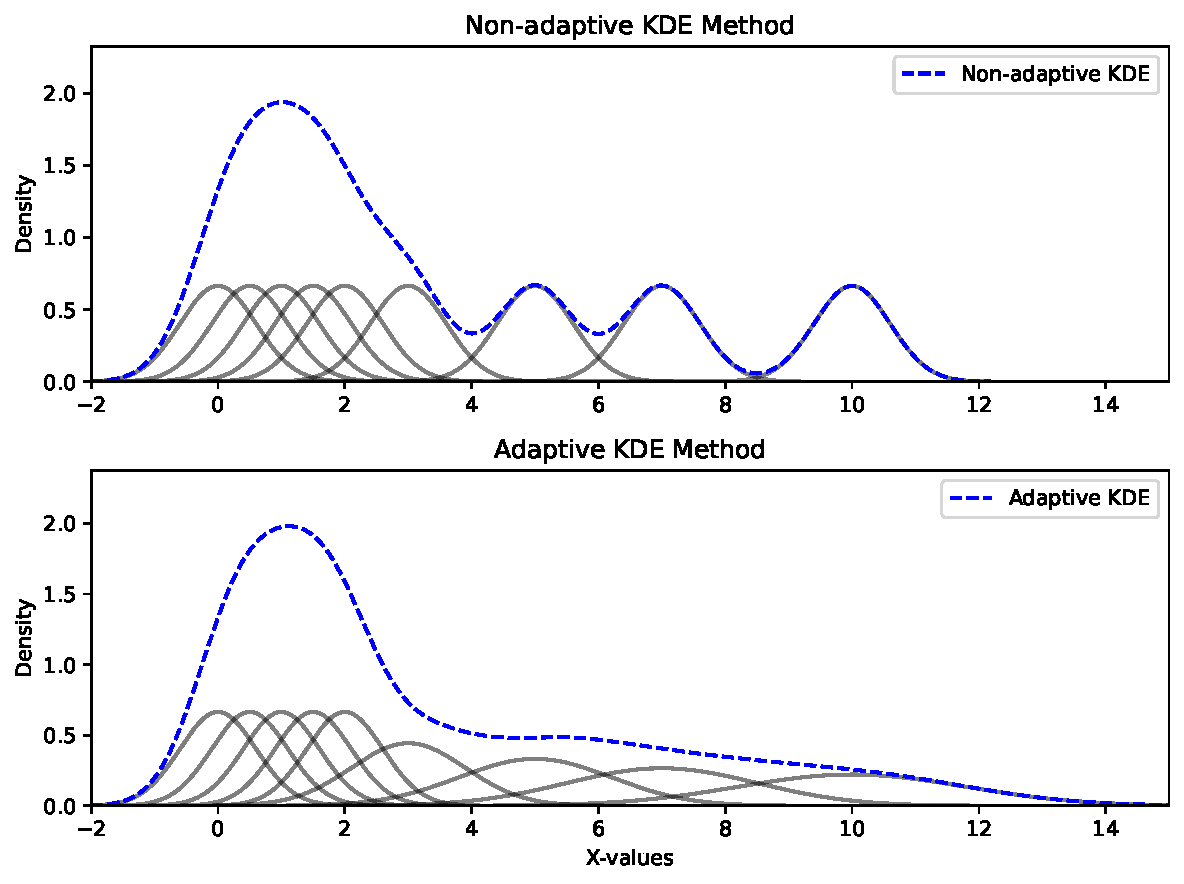
\includegraphics[width=0.6\linewidth]{4_photonid/ffs/smoothing/kde}
    \caption{Esquema del suavizado no adaptativo y adaptativo del m\'etodo \ac{KDE}.}
    \label{fig:ss_corrections:ffs:calculation:adaptive_nonadaptive_kde}
\end{figure}

\begin{figure}[ht!]
    \centering
    \begin{subfigure}[h]{0.49\linewidth}
        \centering
        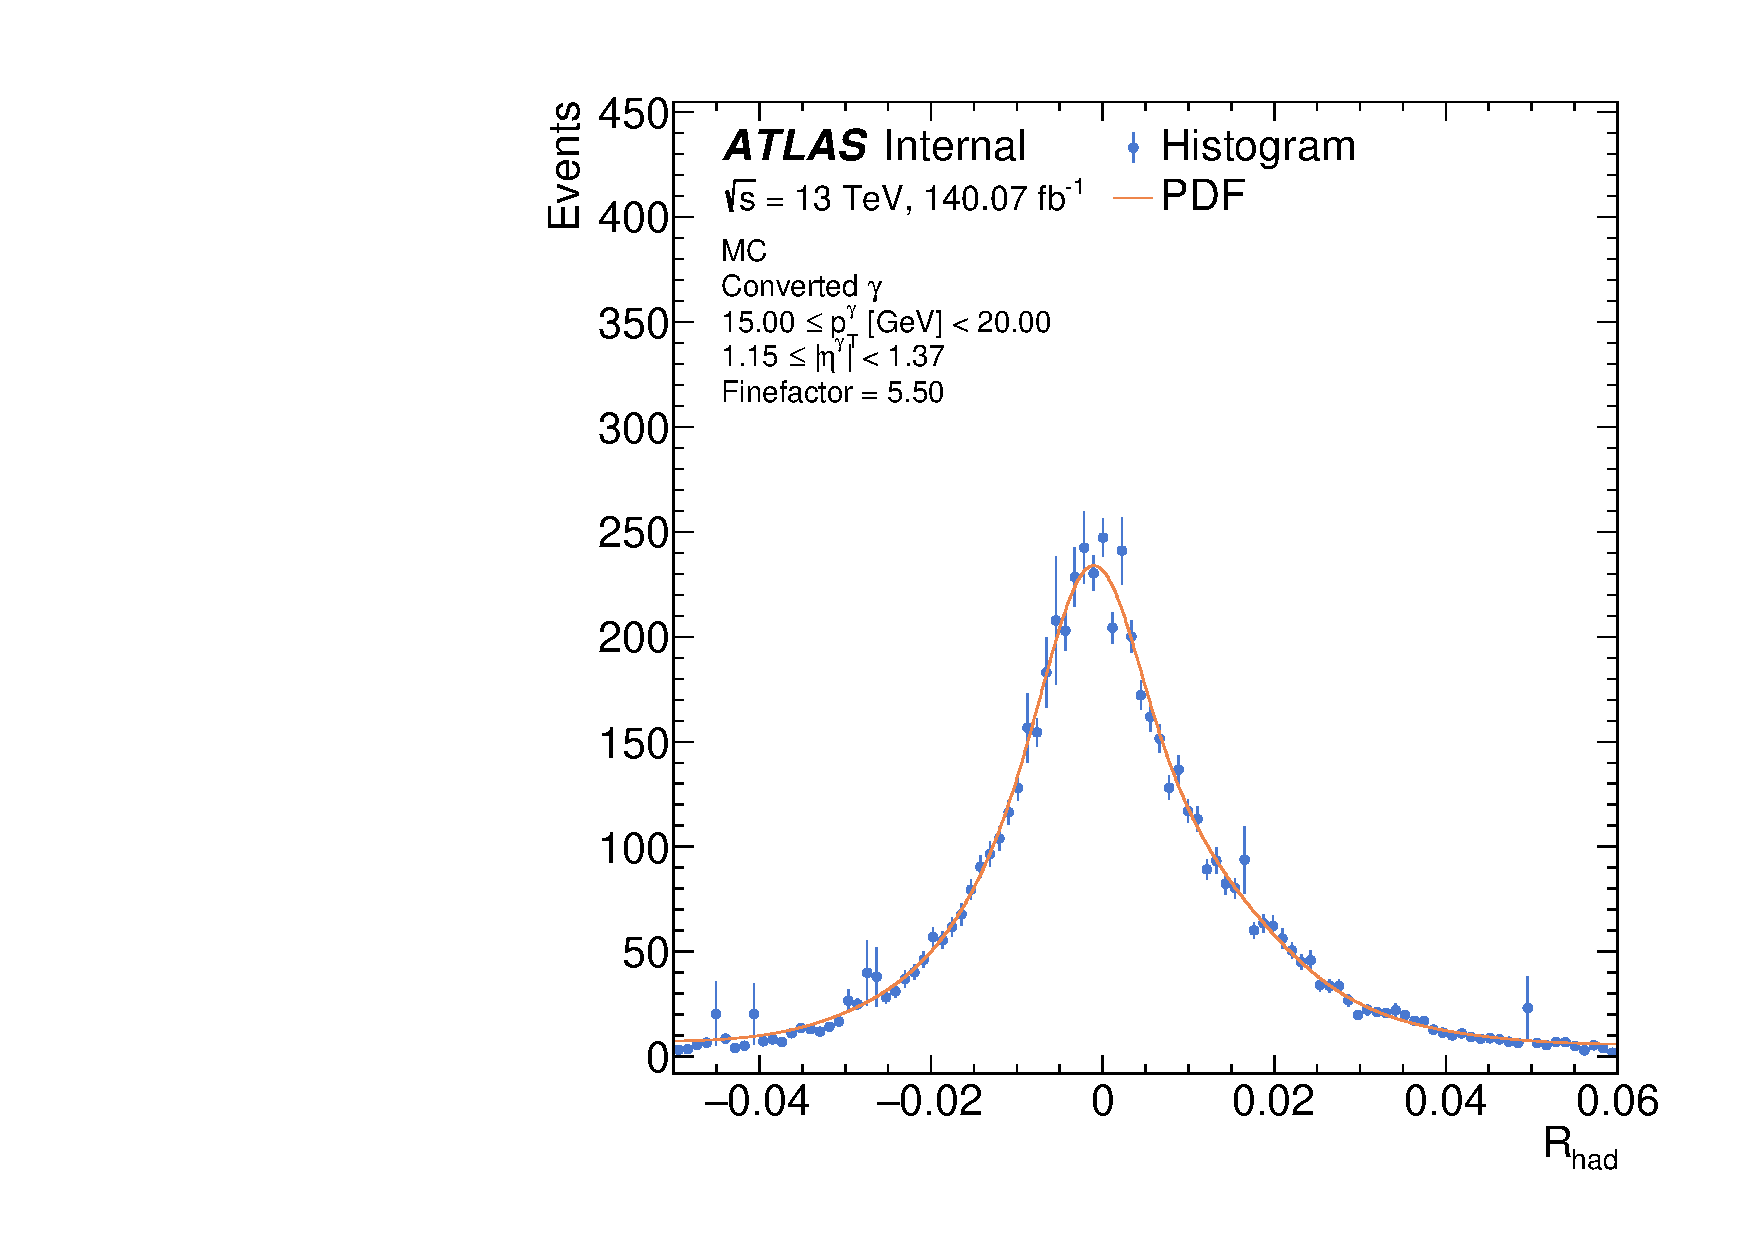
\includegraphics[width=\linewidth]{4_photonid/ffs/smoothing/can__pdfhist__mc__ph_rhad1__c_pt15p0_eta1p15}
        \caption{Caso de baja estad\'istica: muestras de \ac{RZ}}
    \end{subfigure}
    \hfill
    \begin{subfigure}[h]{0.49\linewidth}
        \centering
        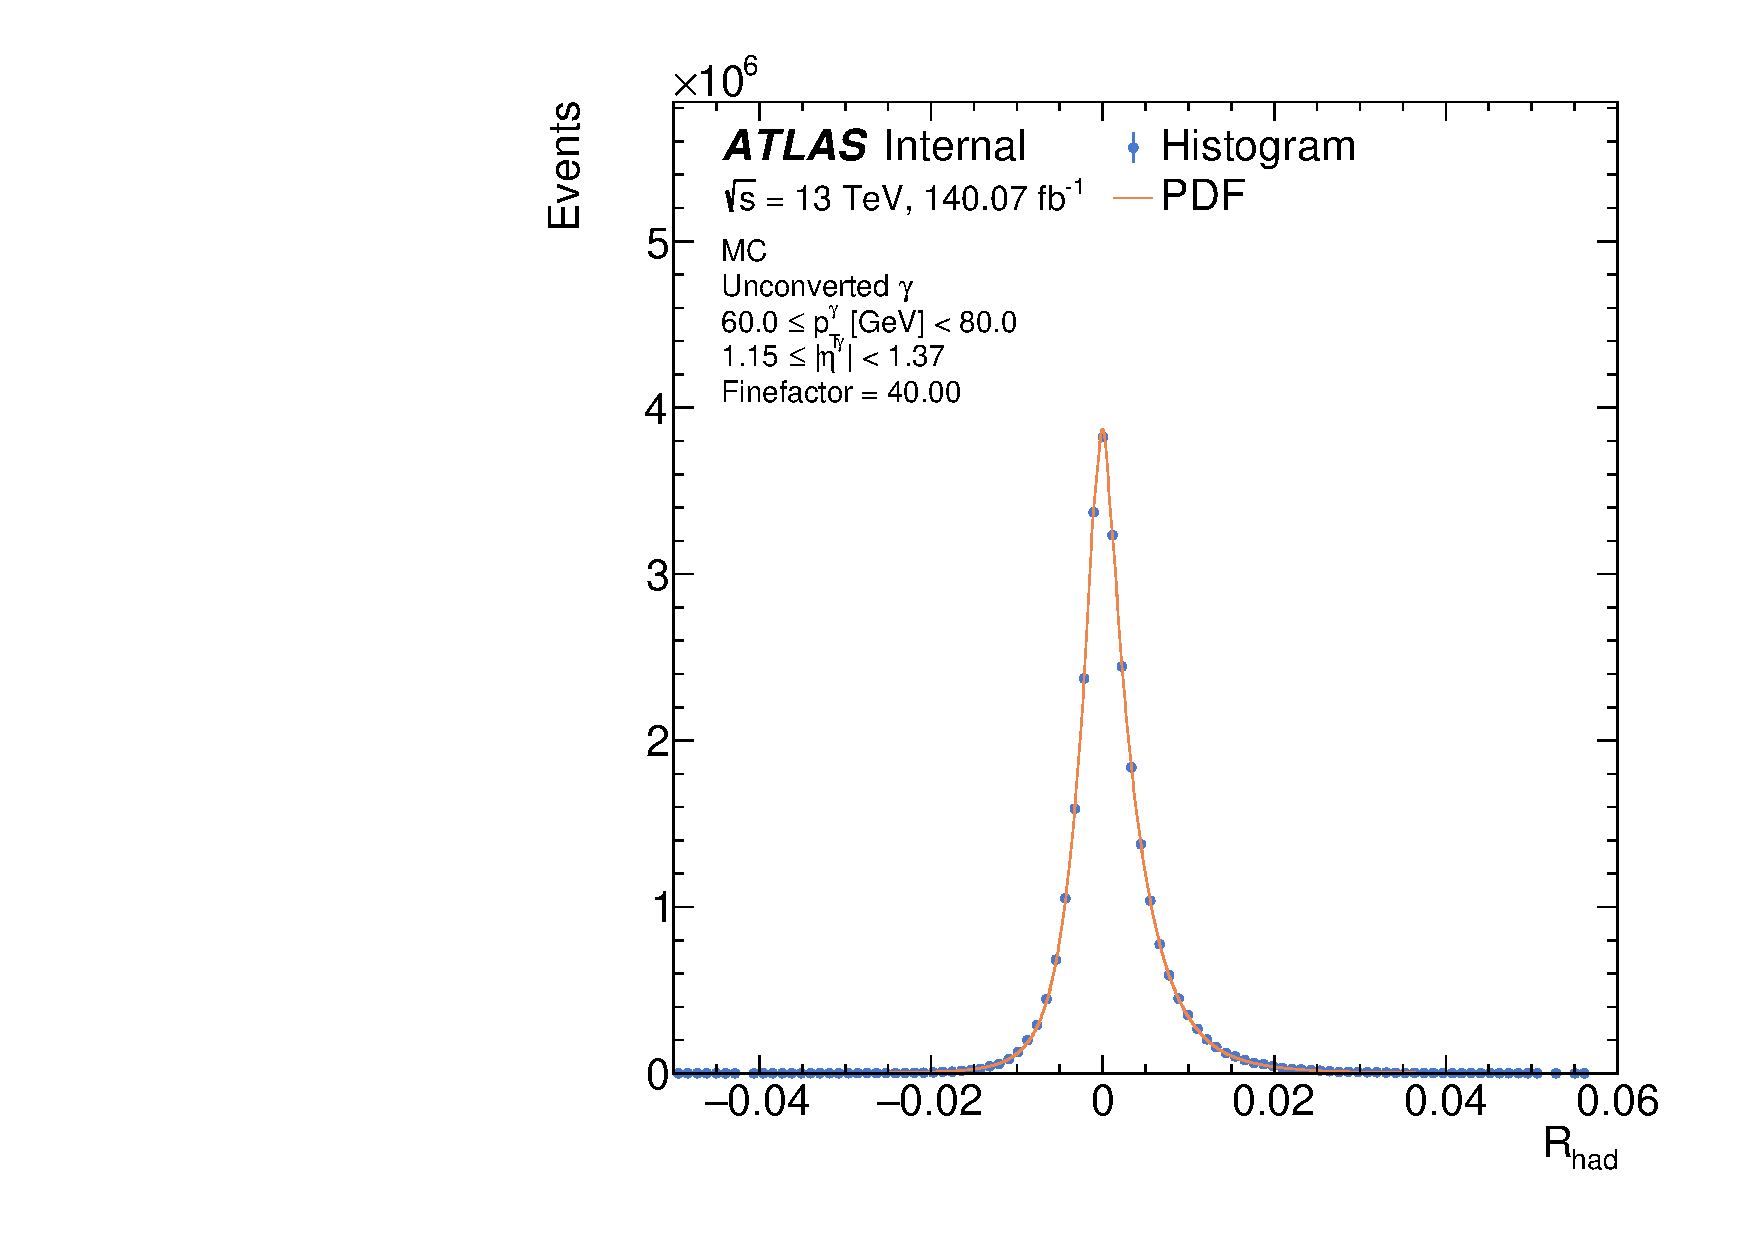
\includegraphics[width=\linewidth]{4_photonid/ffs/smoothing/can__pdfhist__mc__ph_rhad1__u_pt0060p0_eta1p15}
        \caption{Caso de alta estad\'istica: muestras de \ac{SP}}
    \end{subfigure}
    \caption{Suavizado utilizando el m\'etodo \ac{KDE} aplicado a la \ac{SS} \rhad para fotones en \(0.8<\abseta<1.15\) bajo dos posibles escenarios: baja y alta estad\'istica. El histograma original se muestra con los puntos azules y las correspondientes \acp{PDF2} con la l\'inea naranja. Adem\'as, se muestran los valores de los fine factors usados en cada caso.}
    \label{fig:ss_corrections:ffs:calculation:smoothing_ss}
\end{figure}


Una vez creados las \acp{PDF2} de los datos y la simulaci\'on \ac{MC} para una dada variable, bin de \pt y \abseta, y tipo de conversión, la \ac{PDF2} de \ac{MC} se normaliza al de los datos y se calcula un valor \chisq entre ambos como~\cite{Chi2Histograms}:
\begin{equation}
	\chisq = \sum_{i=1}^{N} \dfrac{(w_{\text{MC},i} W_{\text{data}} - w_{\text{data},i} W_{\text{MC}})^2}{s_{\text{MC},i}^2 W_{\text{data}}^2 + s_{\text{data},i}^2 W_{\text{MC}}^2}.
\end{equation}
\(N\) es el número de bines de las \acp{PDF2}, \(w_{\text{MC},i}\) y \(w_{\text{data},i}\) son los números de eventos de \ac{MC} y datos en cada bin, respectivamente, \(s_{\text{MC},i}\) y \(s_{\text{data},i}\) son los errores del bin y, por último, \(W_{\text{data}}\) y \(W_{\text{MC}}\) son la suma de los pesos en datos y \ac{MC}, respectivamente.

\subsubsection{Correcciones \textit{shift-only}}

Como ha sido mencionado anteriormente, las correcciones a las \acp{SS} de \ac{MC} han sido realizadas a partir de simples corrimientos de ellas. Estos corrimientos o desplazamientos se denominan, de aqu\'i en adelante, \textit{shift fugde-factors} \ac{FF}, o simplemente \textit{shifts}.
Para ello, se desplaza a la \ac{PDF2} de \ac{MC} a la izquierda y a la derecha un bin a la vez.
El número inicial de bines que se debe desplazar a la distribución \ac{MC} se calcula mediante la diferencia de los valores medios de las distribuciones de datos y \ac{MC}. A partir de este valor inicial, se consideran shifts de 100 bines a cada lado.
Como consecuencia de este procedimiento, la resolución del shift depende directamente del ancho del bin de la \acp{PDF2}, por lo que bines m\'as pequeños conducen a una mejor resolución del shift. Dado que los histogramas, en primer lugar, se construyen con bines relativamente anchos, la \acp{PDF2} puede construirse utilizando bines pequeños de alta precisión para asegurar una alta resolución. Después de pruebas de convergencia de los \acp{FF}, se decide construir las \acp{PDF2} con 5000 bines.

Para cada bin que se ha desplazado la distribución, se calcula y se registra el valor \chisq antes mencionado. Suponiendo que los errores \(s_{\text{MC},i}\) y \(s_{\text{data},i}\) tienen una distribución gaussiana est\'andar~\footnote{Este requsito se cumple siempre que los contenidos de los bines de ambas \acp{PDF2} sean mayores que 10, lo que también se satisface puesto que los histogramas se construyen con bines relativamente amplios.}, se espera que la forma seguida por los valores \chisq cerca del m\'inimo sea aproximadamente parab\'olica.

Para extraer los \acp{FF}, se realiza un ajuste a los valores de \chisq cercanos al mínimo (5 bines a cada lado del bin mínimo) utilizando una función parabólica y el \ac{FF} de shift se obtiene a partir del mínimo ajustado. Por último, utlilizando este valor, se puede corregir a la \acp{SS} evento a evento como:
\[
	x = x_{\text{old}} + \text{shift}.
\]
donde \(x_{\text{old}}\) y \(x\) representan el valor original y el valor post-correcci\'on de la variable la cual se quiere corregir, respectivamente.


\subsubsection{Correcciones \textit{shift+stretch}}

Se observó que incluso después de aplicar correcciones de shift a las \acp{SS} de \ac{MC}, seguían existiendo diferencias en las formas de las mismas, y en algunos casos éstas pueden ser bastante sustanciales. Una forma de seguir mejorando el acuerdo entre los datos y \ac{MC} es incluir otra corrección que se denomina \textit{stretching}. Las dos correcciones, actuando en conjunto, son denominadas como correcciones shift+stretch (o desplazamiento+estiramiento), que pretenden corregir simultáneamente el valor medio y los anchos de las distribuciones de \ac{MC}.

El método de corrección shift+stretch empieza por encontrar el máximo de la \ac{PDF2} de \ac{MC}. Posteriormente, la \ac{PDF2} se estira al alrededor del m\'aximo calculando la nueva posición de cada bin por el producto \(\text{stretch}\times (x - \text{stretch point})\), donde \(x\) es el centro del bin en cuesti\'on. De este modo, el centro de cada bin conserva la distancia inicial al centro de la distribución, multiplicada por el factor de stretch. En el escenario en el que el stretch es \(>1\), puede haber casos en los que sea lo suficientemente grande como para dar lugar a bines vacíos. El contenido de estos bines vacíos se interpola linealmente a partir de los bines vecinos distintos de cero.
Una vez \textit{estirada} la \ac{PDF2}, se desplaza a izquierda y derecha siguiendo el mismo procedimiento que para el caso de shift-only, calculando los valores \chisq para cada \(\text{shift}_i\) después de aplicar el \(\text{stretch}_j\). Como resultado de este procedimiento, ahora se obtiene una grilla bidimensional de valores de \chisq en el plano de shift-stretch. El par shift-stretch se obtiene del el centro del bin mínimo, y comprenden ahora los \acp{FF}. Las correcciones pueden ser aplicadas a cada \ac{SS} \(x\), evento a event, como:
\begin{equation}
	x = \text{stretch}\times(x_{\text{old}} - \text{stretch point}) + \text{shift} + \text{stretch point},
\end{equation}
donde nuevamente \(x_\text{old}\) representa el valor de la variable sin corregir.

Un ejemplo de los valores de \chisq resultantes para la variable \fside se muestra en la \Fig{\ref{fig:ss_corrections:ffs:calculation:fside_calculation:chi2}}, donde el shift est\'a representado en el eje \(x\) y el stretch en el eje \(y\). El valor óptimo de shift-stretch en este caso corresponde a \(\text{shift}=0.03\) y \(\text{stretch}=1.09\). En la \Fig{\ref{fig:ss_corrections:ffs:calculation:fside_calculation:pdfs}} se muestran las \acp{PDF2} antes y después de aplicar las correcciones, donde se comparan con la \ac{PDF2} de los datos. Como se ve en la figura, hay una gran mejora y las distribuciones coinciden casi a la perfección.

\begin{figure}[ht!]
    \centering
    \begin{subfigure}[t]{0.49\linewidth}
        \centering
        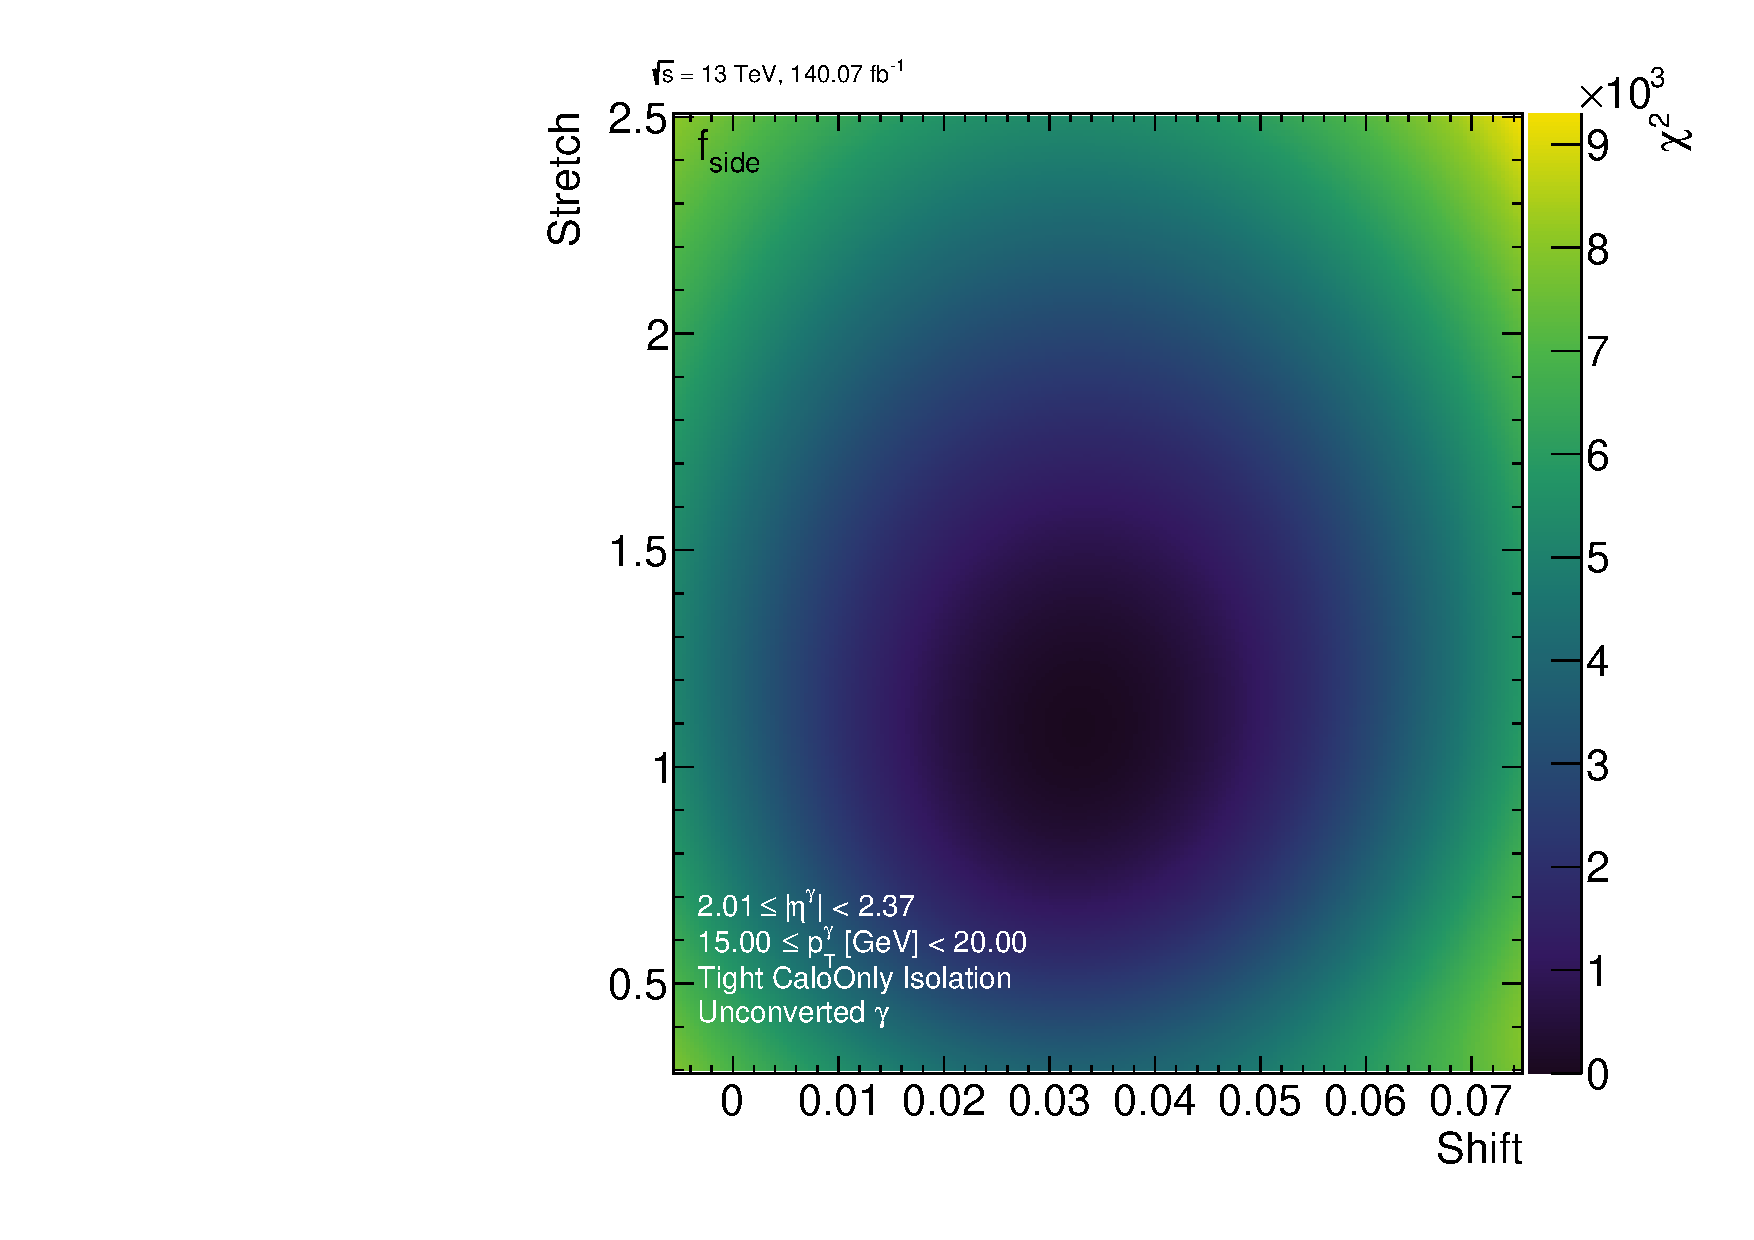
\includegraphics[width=\linewidth]{4_photonid/ffs/procedure/can2d__chi2scan_nocontour__ph_fside__Isotightcaloonly_IdNone_u_pt15p0_eta2p01}
        \caption{Valores de \chisq en el plano shift-stretch.}
        \label{fig:ss_corrections:ffs:calculation:fside_calculation:chi2}
    \end{subfigure}
    \hfill
    \begin{subfigure}[t]{0.49\linewidth}
        \centering
        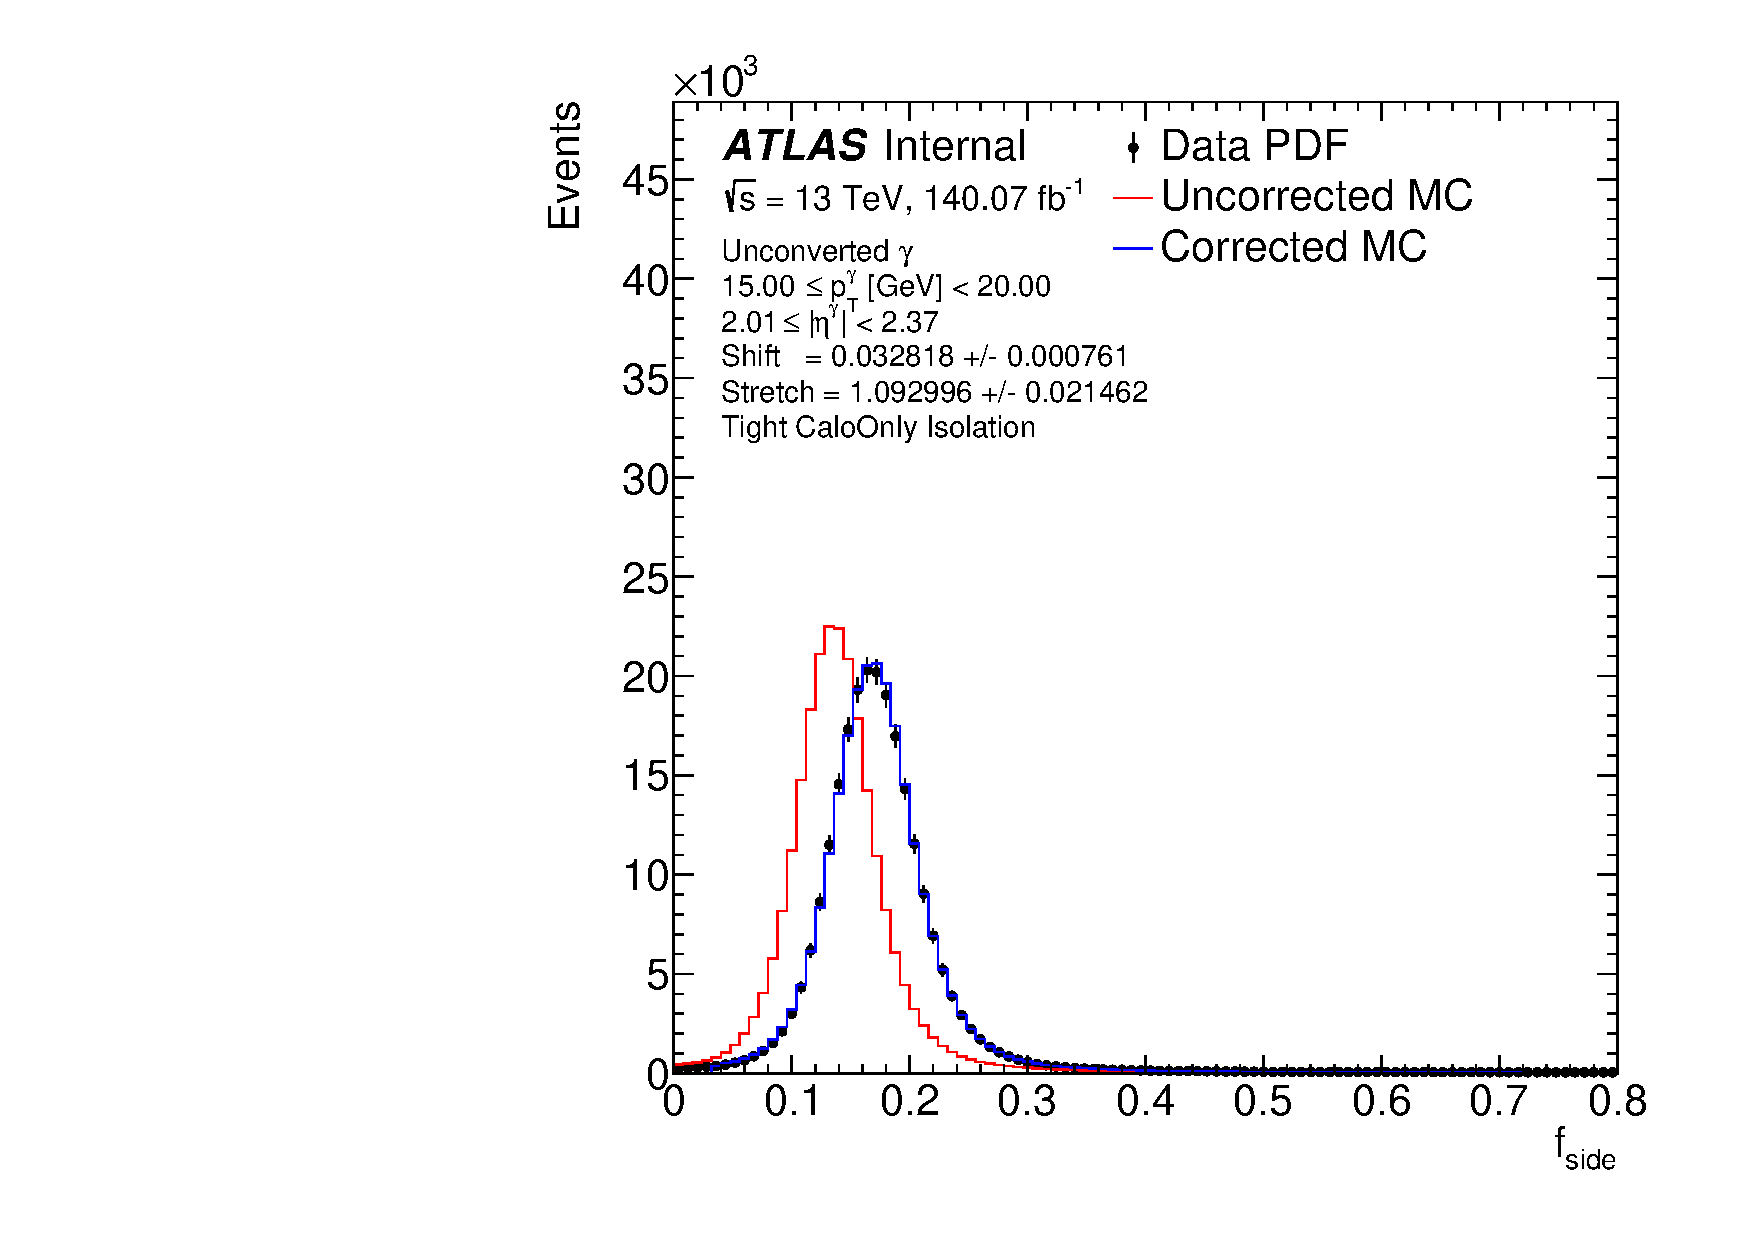
\includegraphics[width=\linewidth]{4_photonid/ffs/procedure/can__data_mc_fudged_comp__ph_fside__Isotightcaloonly_IdNone_u_pt15p0_eta2p01}
        \caption{\acp{PDF2} de datos (puntos negros) y simulaci\'on \ac{MC} sin corregir (l\'inea roja) y corregida (l\'inea azul), mostrando el impacto de las correcciones.}
        \label{fig:ss_corrections:ffs:calculation:fside_calculation:pdfs}
    \end{subfigure}
    \caption{C\'alculo de los \acp{FF} de shift+stretch para \fside utilizando fotones no convertidos con momento transverso de \(15<\pt<20~\gev\) y pseudorapidez \(2.01<\abseta<2.37\) }
    \label{fig:ss_corrections:ffs:calculation:fside_calculation}
\end{figure}







\subsection{C\'alculo de incertezas}
\label{subsec:ss_corrections:ffs:uncs}

\subsubsection{Incertezas estad\'isticas}

Para extraer las incertezas estadísticas de los \acp{FF} de shift y stretch, se realiza un ajuste al contorno de \(1\sigma\) (nivel de confianza del \(68.3\%\)) sobre los valores \chisq. Este contorno representa una elipse que toma la siguiente forma:
\begin{equation}
    \chi^2 = \chi^2_{\text{min}} + \frac{1}{1-\rho^2} \left[ \left( \frac{x-x_0}{\sigma_x} \right)^2 + \left( \frac{y-y_0}{\sigma_y} \right)^2 - 2\rho \left( \frac{x-x_0}{\sigma_x} \right) \left( \frac{y-y_0}{\sigma_y} \right) \right],
\end{equation}
donde \(\rho\) es el coeficiente de correlación entre ambas variables, \(\sigma_x\) y \(\sigma_y\) las incertezas sobre \(x\) y \(y\), respectivamente, \((x_0, y_0)\) es la posici\'on del centro de la elipse, y \(\chi^2_{\text{min}}\) es el valor mínimo de \(\chi^2\) obtenido del histograma bidimensional.


Extrayendo los semiejes mayor y menor de la elipse ajustada, y con el ángulo de inclinación de la misma, las incertezas estadísticas sobre dos variables \(x\) y \(y\) (que en este caso representan el shift y el stretch, respectivamente) son (véase el \App{\ref{app:ellipse_formulae}}):
\begin{gather}
    \sigma_x = \sqrt{a^2 \cos^2\theta + b^2 \sin^2\theta}\\
    \sigma_y = \sqrt{a^2 \sin^2\theta + b^2 \cos^2\theta}.
\end{gather}

\subsubsection{Incertezas sistem\'aticas}

Las incertezas sistemáticas se obtienen variando los criterios de preselección, es decir, la identificación y el aislamiento de fotones. El cambio de los diferentes criterios de preselección permite que las \acp{SS} varíen dependiendo de la cantidad de contaminación de fondo, y en consecuencia también lo hacen los \acp{FF}.
Las diferentes selecciones son, para cada muestra:
\begin{itemize}
    \item \acf{RZ}:
        \begin{itemize}
            \item Nominal: Sin criterio de identificaci\'on, aislamiento \texttt{FixedCutTightCaloOnly}.
            \item Identificación loose, sin aislamiento.
            \item Identificación loose, aislamiento \texttt{FixedCutTightCaloOnly}.
            \item Sin identificación, aislamiento \texttt{FixedCutLoose}.
        \end{itemize}
    \item \acf{SP}:
        \begin{itemize}
            \item Nominal: identificaci\'on tight, aislamiento \texttt{FixedCutLoose}.
            \item identificaci\'on tight, aislamiento \texttt{FixedCutTight} .
        \end{itemize}
\end{itemize}
Todas las demás combinaciones (o falta de ellas) de criterios de selección darían como resultado una muestra con estadísticas demasiado bajas o una muy baja pureza.

Los \acp{FF} se derivan para cada una de las selecciones anteriores, y se calcula la diferencia entre la nominal y la variada. La diferencia máxima se toma como incerteza sistemática, como el caso más conservativo. Finalmente, las incertezas estad\'isticas y sistem\'aticas se suman en cuadratura.










\subsection{Resultados}
\label{subsec:ss_corrections:ffs:results}


Debido al hecho de que los \acp{FF} se calculan en un amplio rango de \pt y utilizando dos muestras distintas que abarcan regiones complementarias, los resultados se concatenan en \(50~\gev\), que coincide con el l\'imite entre ellas.

A continuación, los valores de shift y stretch para distintas \acp{SS} ser\'an mostrados. Los valores de shift se normalizan utilizando la desviaci\'on est\'andar de la \ac{SS} luego de aplicar el \ac{FF} de stretch, ya que esta cantidad permite comprender cuánto se desplaza cada variable con respecto a su ancho. Además, proporciona una medida única para todas las variables consideradas, ya que cada una de ellas abarca rangos diferentes. No obstante, el ancho de las variables varía según los distintos bines de \pt y \abseta, lo que puede dar lugar a grandes diferencias entre bines vecinos.
%En tales casos, no hay diferencias drásticas con respecto a los valores de shift originales, trat\'andose s\'olo de diferencias en los anchos de las distribuciones.

En la \Fig{\ref{fig:ss_corrections:ffs:reslts:ffs}}, se presentan ejemplos de los \acp{FF} resultantes para las variables \reta y \weta utilizando fotones convertidos. Se puede observar que para ambas variables los \acp{FF} dependen de \pt, especialmente hacia momentos transversos más altos. Este comportamiento también se repite en todas las variables.
Inspeccionando los comportamientos y tendencias de los \acp{FF}, también es posible recuperar información sobre el mal modelado de las \acp{SS} por el \ac{MC}. Como se mencion\'o en la \Sect{\ref{sec:pid_ss:ss_differences}}, se observaron anchos y perfiles en \(\eta\) más amplios para los datos en comparación con la simulación. De hecho, esto se puede inferir dado los valores de stretch aumentan hacia valores más altos de \pt, estirando las simulaciones \ac{MC} hasta el doble de su ancho inicial. En el caso de \reta (\weta) mostrado, la simulación \ac{MC} sobreestima (subestima) el valor central de la distribuci\'on en casi una desviación estándar después de corregir la ancho, lo que significa que las diferencias entre la distribución \ac{MC} sin corregir con la de los datos son muy grandes.

\begin{figure}[ht!]
    \centering
    \begin{subfigure}[h]{0.49\linewidth}
        \centering
        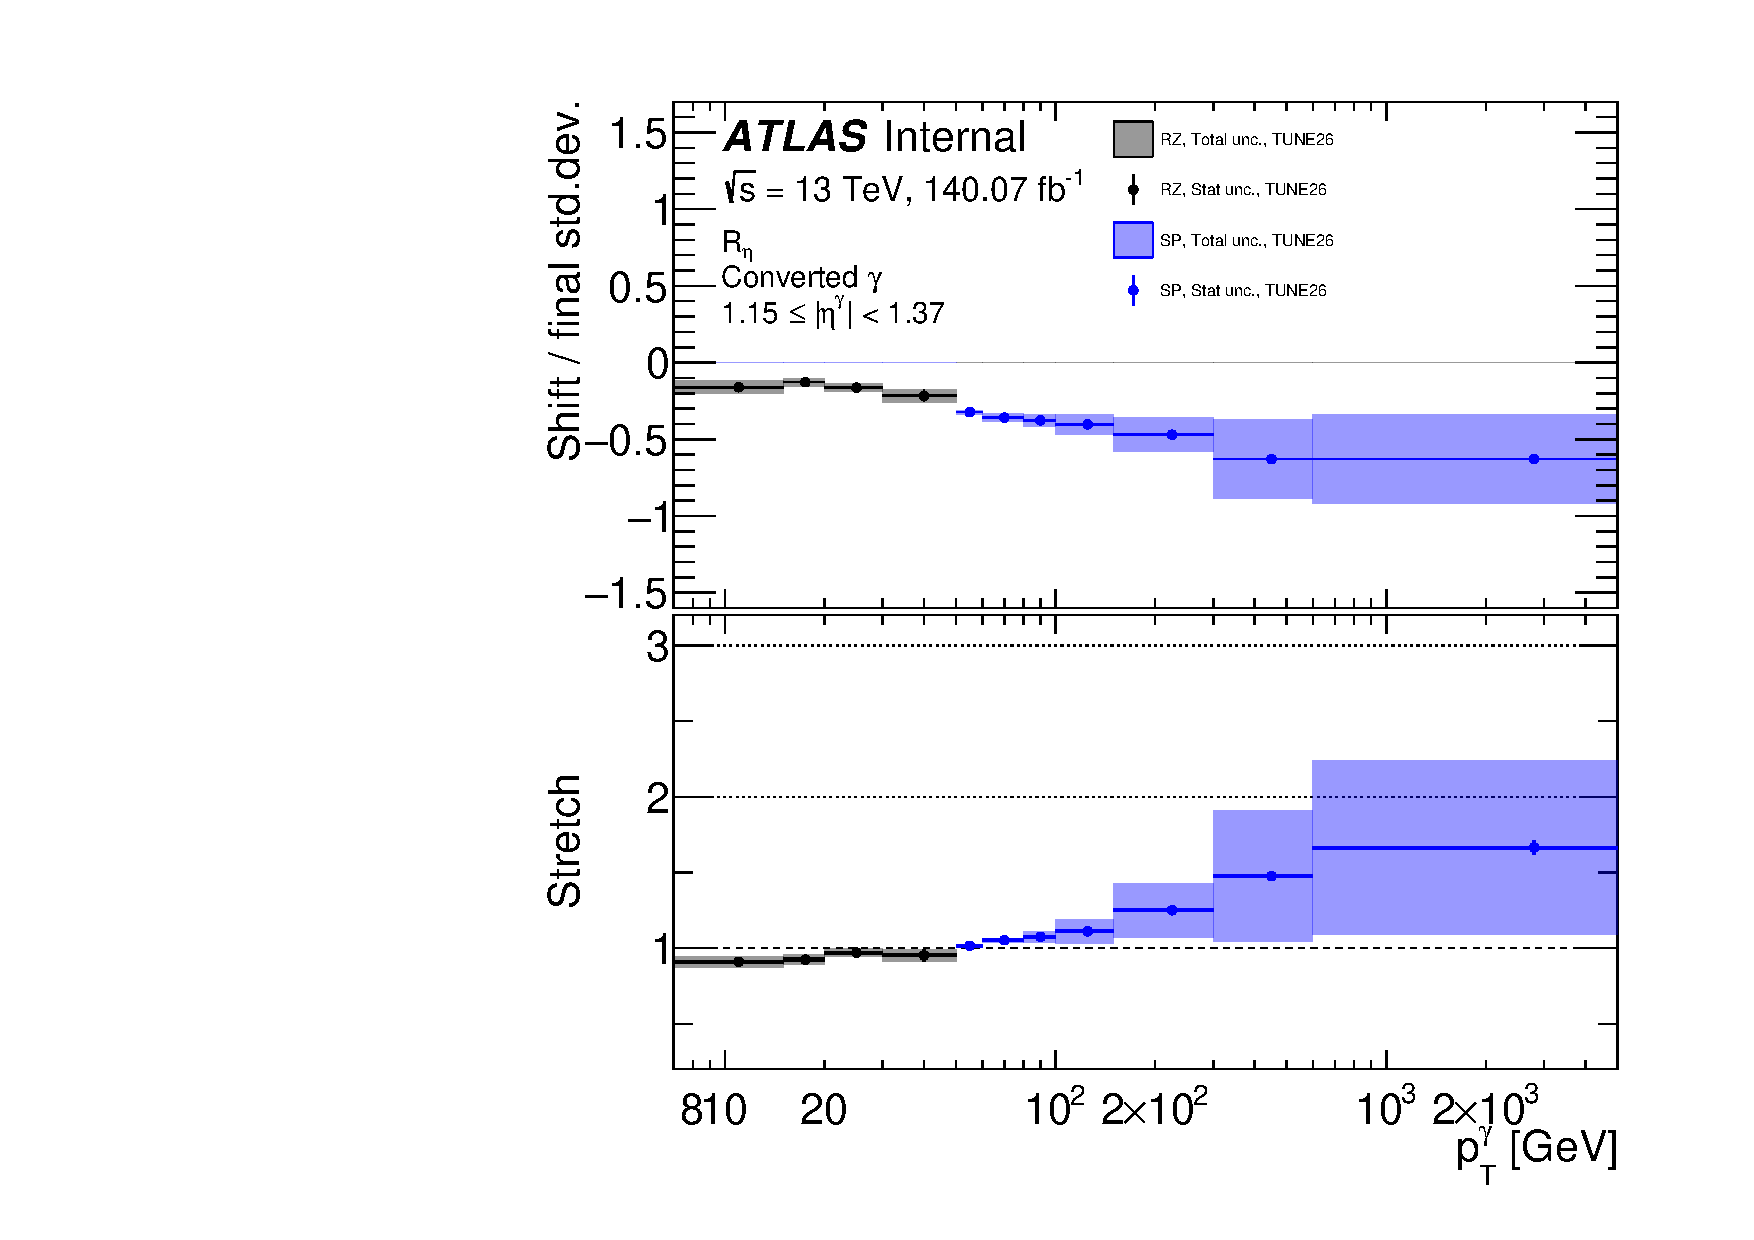
\includegraphics[width=\linewidth]{4_photonid/ffs/results/combined/1d/can__comb__ph_reta__c__eta1p15__shift_normalized}
        \caption{\reta}
        \label{fig:ss_corrections:ffs:reslts:ffs:reta}
    \end{subfigure}
    \hfill
    \begin{subfigure}[h]{0.49\linewidth}
        \centering
        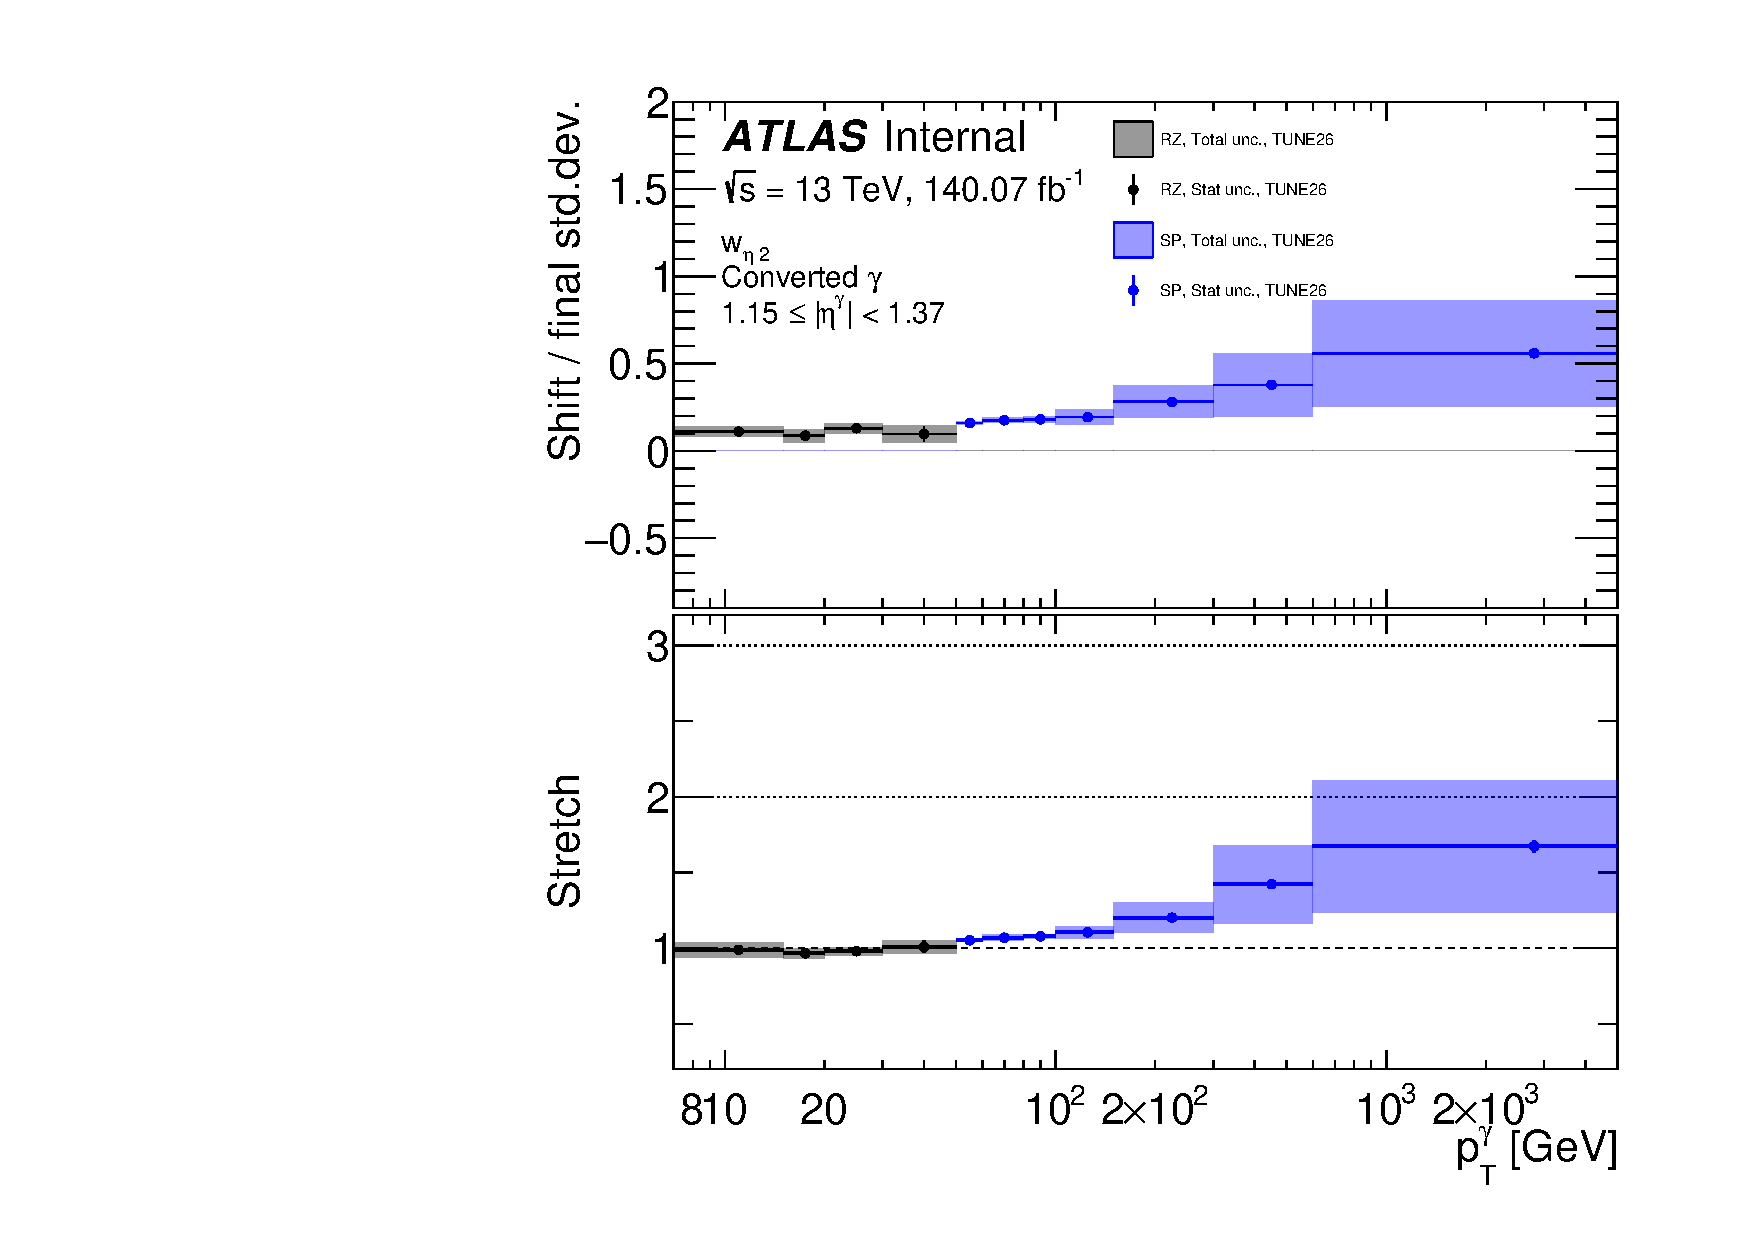
\includegraphics[width=\linewidth]{4_photonid/ffs/results/combined/1d/can__comb__ph_weta2__c__eta1p15__shift_normalized}
        \caption{\weta}
        \label{fig:ss_corrections:ffs:reslts:ffs:weta}
    \end{subfigure}
    \caption{Valores de los \acp{FF} de shift y stretch para las \reta (izquierda) y \weta (derecha) para fotones convertidos con \(1.15<\abseta<1.37\), en funci\'on de \pt. Los resultados obtenidos por las muestras de \ac{RZ} est\'an representados por el color negro, mientras que los resultados de \ac{SP} se muestran en azul. Los puntos y las l\'ineas denotan los valores centrales con sus incertezas estad\'isticas, mientras que las regiones sombreadas representan las incertezas totales. Los valores de shift se muestran en el panel superior, los cuales son normalizados por el ancho de la distribuci\'on luego de ser estirada por el stretch, como se ha explicado en el texto. Este \'ultimo valor se muestra en el panel inferior de las figuras.}
    \label{fig:ss_corrections:ffs:reslts:ffs}
\end{figure}

También es útil visualizar los \acp{FF} en un bin de \pt fijo y en función de \abseta, para as\'i determinar qu\'e tan dependientes de \abseta son las correcciones. Esto se muestra para \wstot utilizando fotones convertidos con \(50<\pt<60~\gev\) en la \Fig{\ref{fig:ss_corrections:ffs:reslts:ffs_eta_wstot}}. Como se puede notar, para \(\abseta>1.81\) (los dos últimos bines), los valores de shift normalizados son mayores que los de los bines anteriores en, al menos, un factor 2. Sin embargo, los valores de shift sin normalizar mostrados en la \Fig{\ref{fig:ss_corrections:ffs:reslts:ffs_eta_wstot:raw_shift}} no presentan un cambio tan brusco, observ\'andose s\'olo una peque\~na dependencia en \abseta. Como consecuencia de este comportamiento, se puede concluir que el cambio brusco observado es debido al cambio en el ancho de la distribuci\'on entre los distintos bines de \abseta., tal como se hab\'ia anticipado.


\begin{figure}[ht!]
    \centering
    \begin{subfigure}[h]{0.49\linewidth}
        \centering
        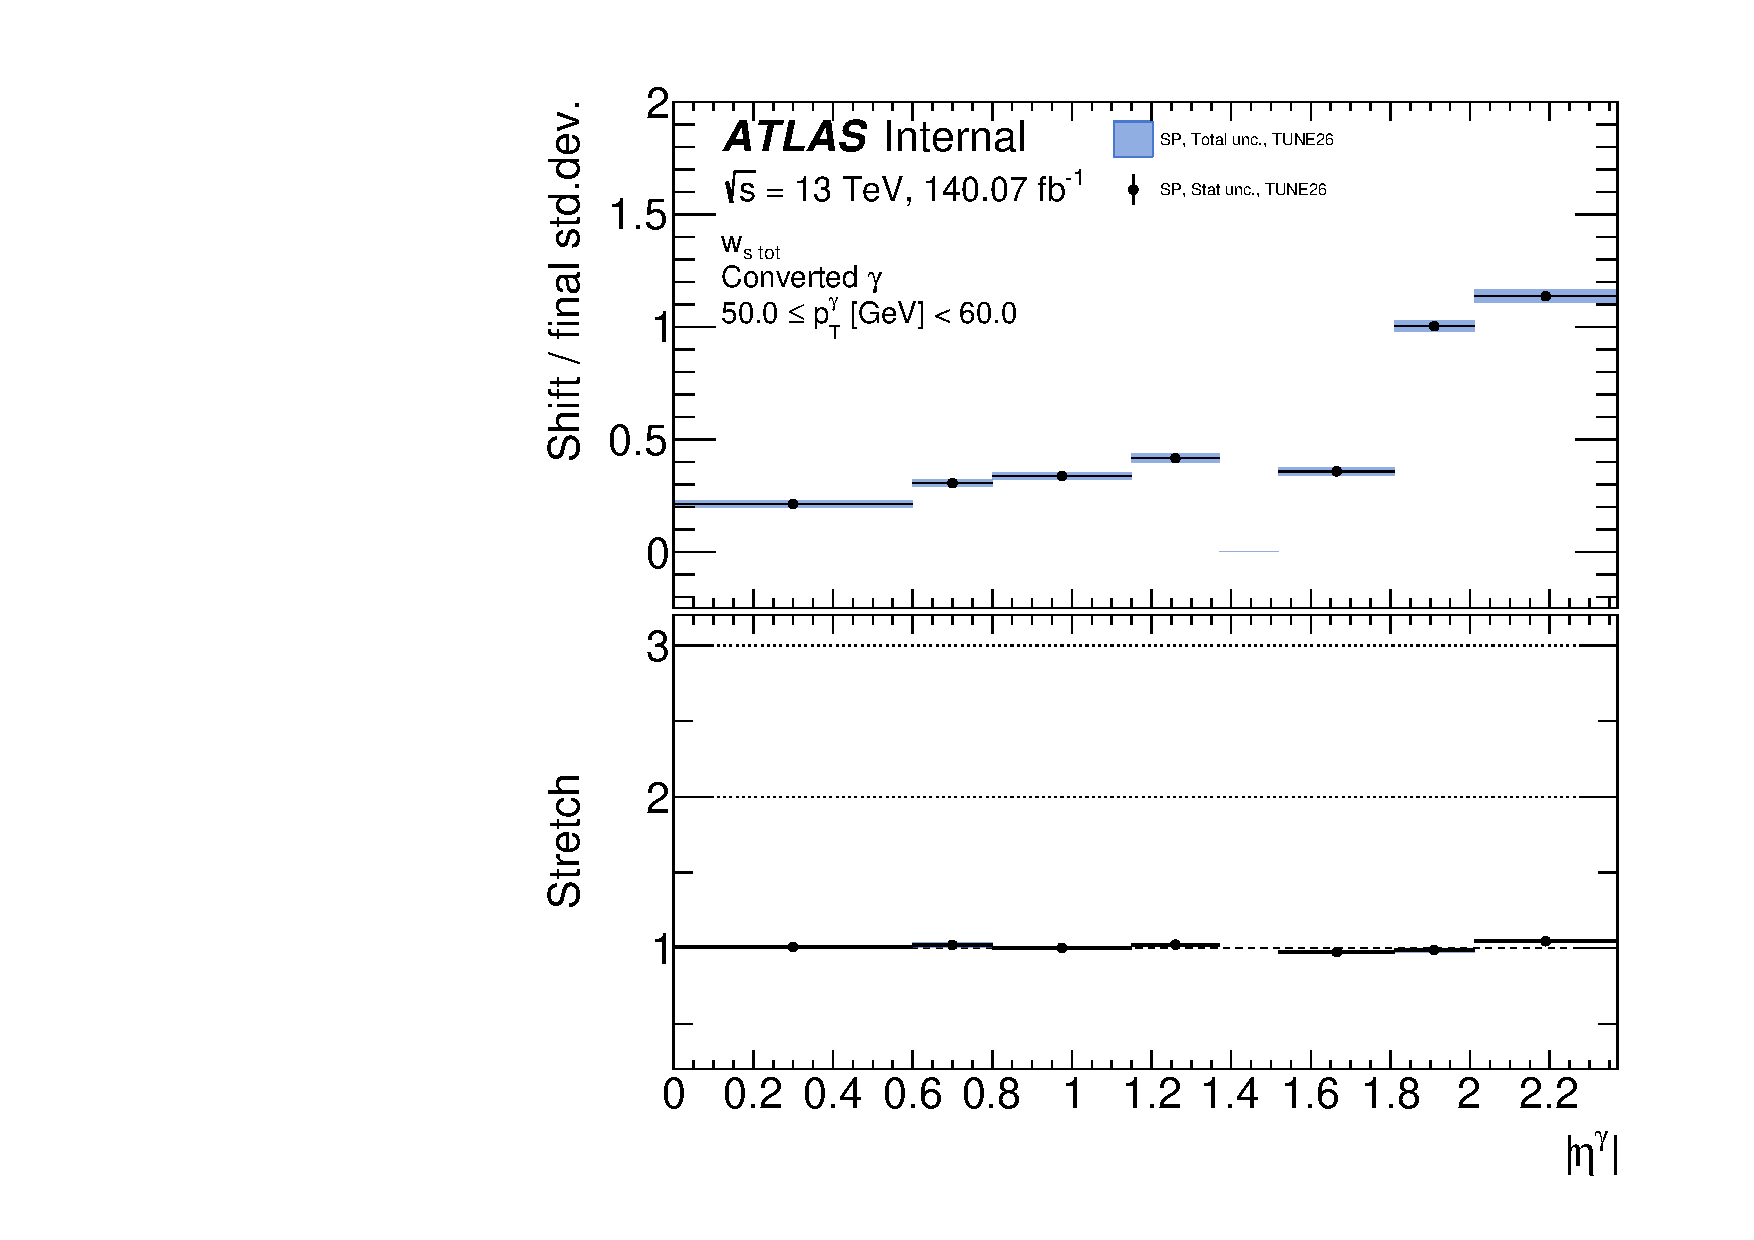
\includegraphics[width=\linewidth]{4_photonid/ffs/results/SP/1d/can__SP__ph_wstot__c__pt0050p0__shift_normalized}
        \caption{Valores de shift normalizados.}
        \label{fig:ss_corrections:ffs:reslts:ffs_eta_wstot:normalised_shift}
    \end{subfigure}
    \hfill
    \begin{subfigure}[h]{0.49\linewidth}
        \centering
        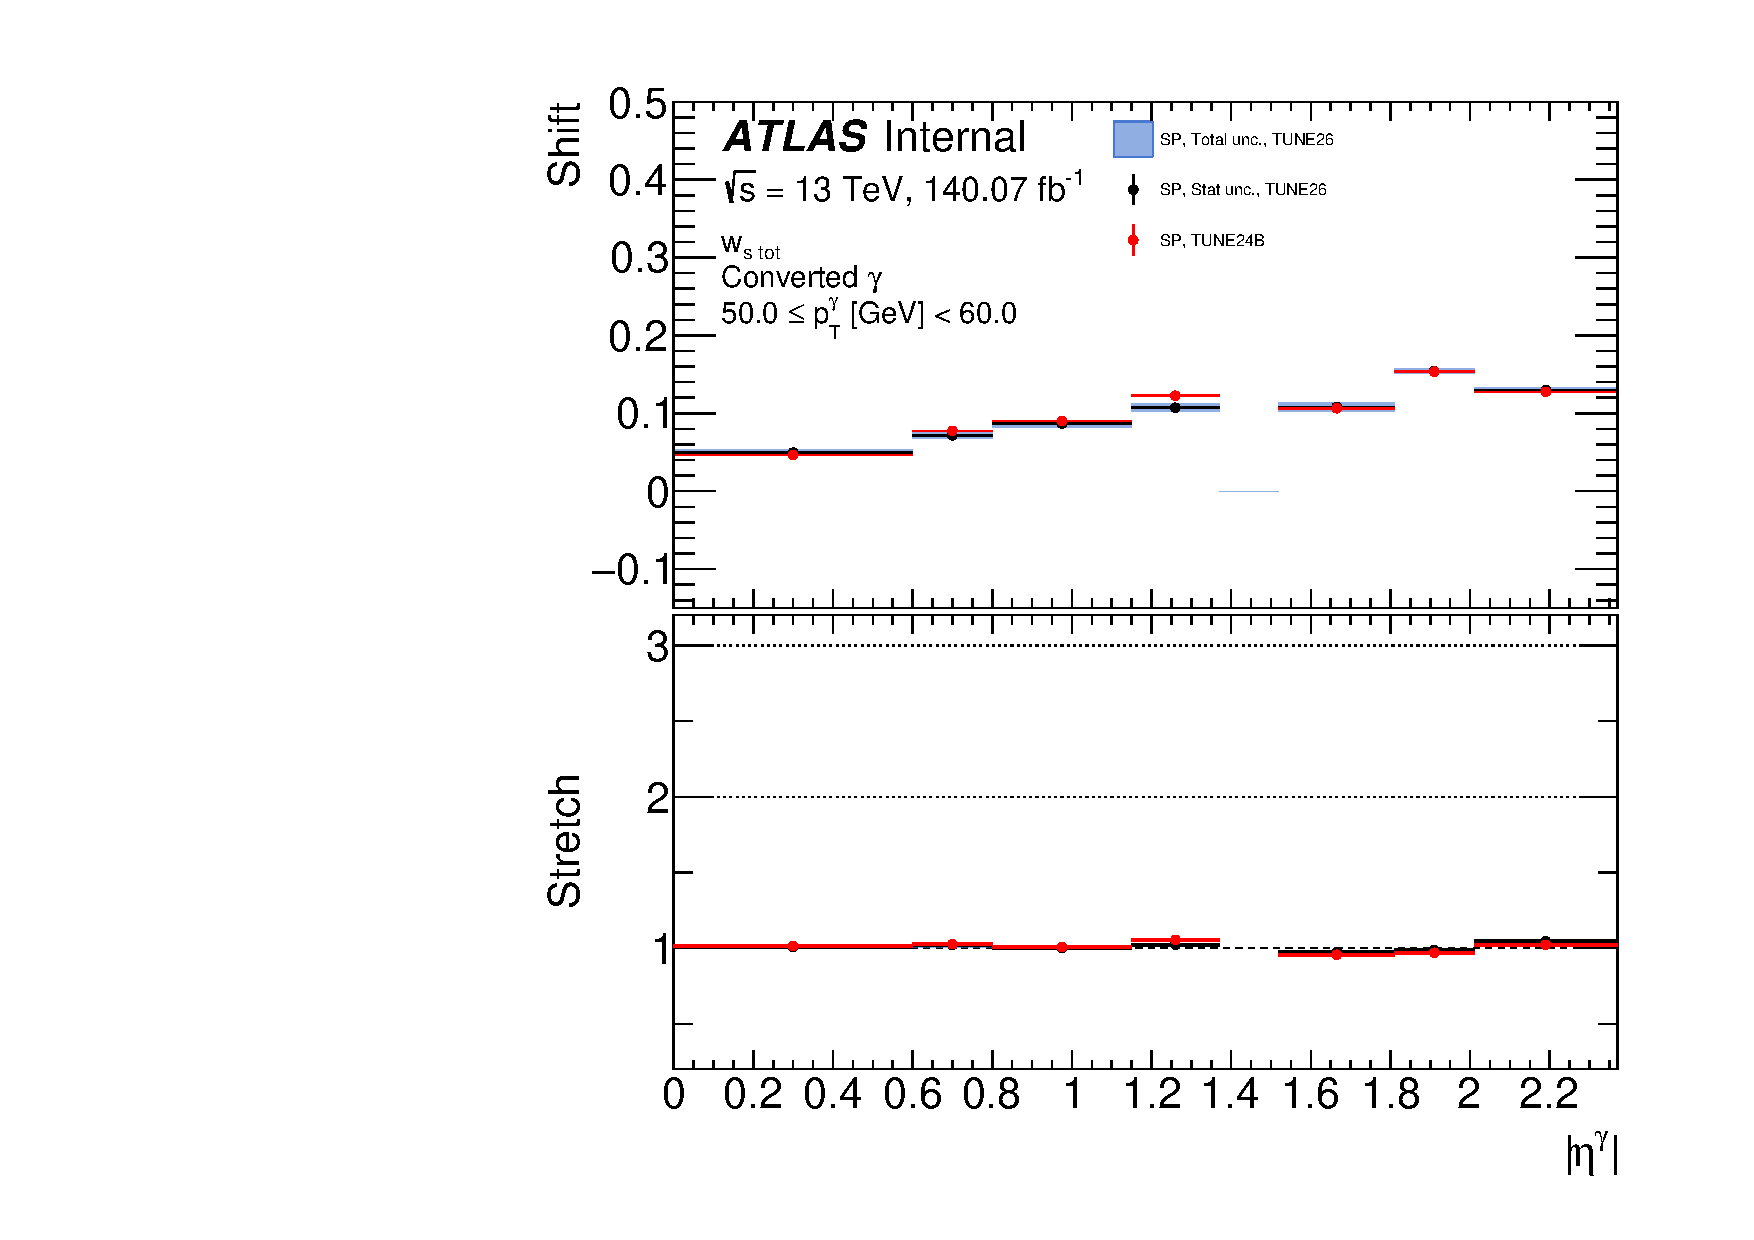
\includegraphics[width=\linewidth]{4_photonid/ffs/results/SP/1d/can__SP__ph_wstot__c__pt0050p0}
        \caption{Valores de shift sin normalizar.}
        \label{fig:ss_corrections:ffs:reslts:ffs_eta_wstot:raw_shift}
    \end{subfigure}\\
    \caption{Valores de los \acp{FF} de shift y stretch para \wstot en funci\'on de \abseta utilizando fotones convertidos con \(50<\pt<60~\gev\) de las muestras de \ac{SP}. La \Fig{\subref{fig:ss_corrections:ffs:reslts:ffs_eta_wstot:normalised_shift}} muestra los valores de shift normalizados, mientras que los no normalizados se encuentra en la \Fig{\subref{fig:ss_corrections:ffs:reslts:ffs_eta_wstot:raw_shift}}. Los puntos con las l\'ineas de color muestran los valores centrales y las incertezas estad\'isticas, mientras que las \'areas sombreadas representan las incertezas totales en cada bin. Los valores de stretch se muestran en los paneles inferiores de cada figura.}
    \label{fig:ss_corrections:ffs:reslts:ffs_eta_wstot}
\end{figure}


Para validar los \acp{FF} obtenidos, las correcciones se aplican a las \acp{SS} evento por evento.
Las \Figs{\ref{fig:ss_corrections:ffs:results:ss_rz}}{\ref{fig:ss_corrections:ffs:results:ss_sp}} muestran la aplicación de los \acp{FF} a algunas de las \ac{SS} utilizando las muestras \ac{RZ} y \ac{SP}, respectivamente, divididas en las regiones barrel y endcap en \abseta. En la región barrel, las correcciones mejoran el acuerdo entre datos y \ac{MC}, pero la mejora no es tan significativa como en la región endcap, donde se observan excelentes acuerdos entre datos y \ac{MC}. Tomando como ejemplo las variables \wone y \wstot, se observan grandes diferencias en las formas entre la simulación nominal y los datos, que los métodos shift+stretch consiguen corregir. El mismo comportamiento se observa con las muestras \ac{SP}, en las que estas variables presentan dos o más picos, y que se corrigen correctamente con el método de \acp{FF}. En todos los casos mostrados, el \ac{MC} corregido y los datos son casi indistinguibles, lo que demuestra la importancia de estas correcciones y cómo logran un excelente acuerdo.

\begin{figure}[ht!]
    \centering
    \begin{subfigure}[h]{0.32\linewidth}
        \centering
        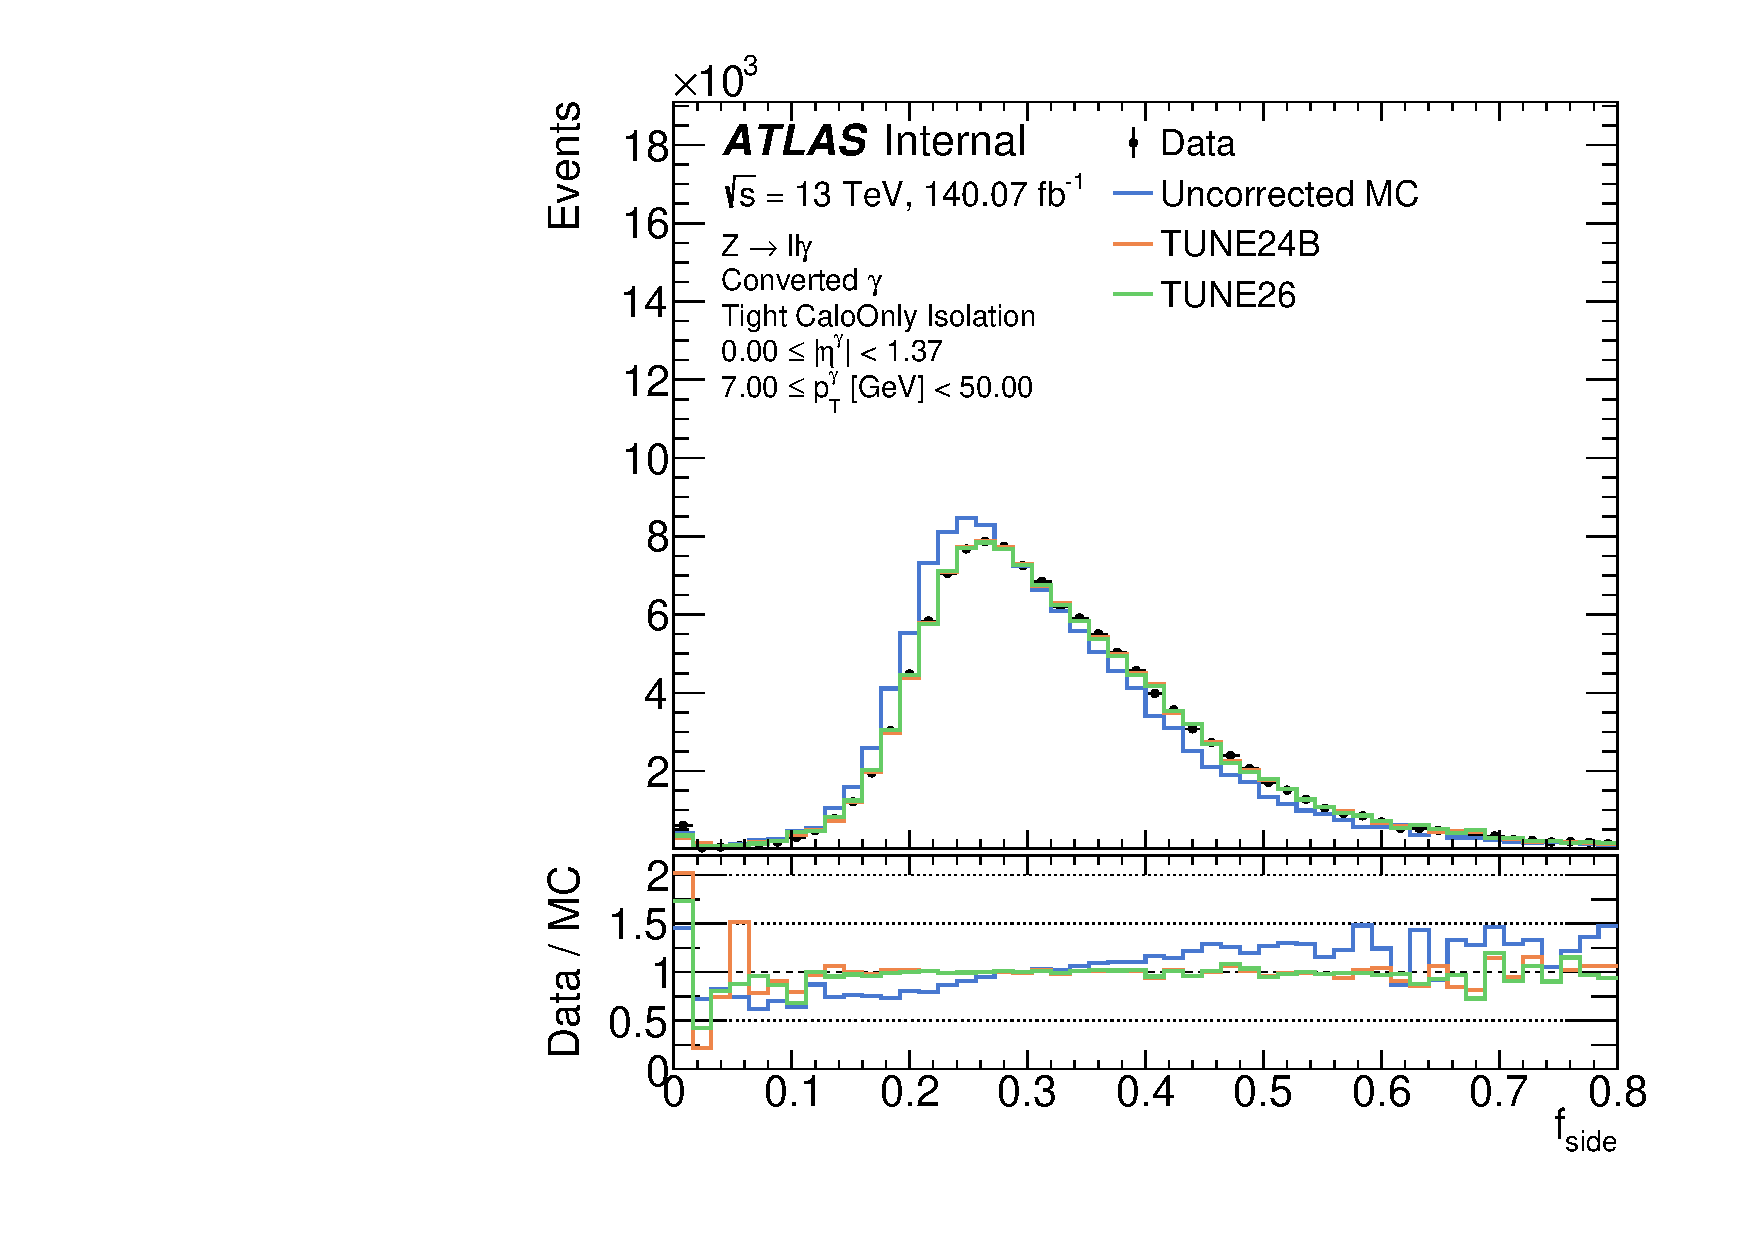
\includegraphics[width=\linewidth]{4_photonid/ffs/results/RZ/corrections/c/ptFull/etaCoarse/can__correction__ph_fside__Isotightcaloonly_IdNone__c__ptFullpt07p0__etaCoarseeta0p00}
        \caption{\fside, barrel.}
    \end{subfigure}
    \hfill
    \begin{subfigure}[h]{0.32\linewidth}
        \centering
        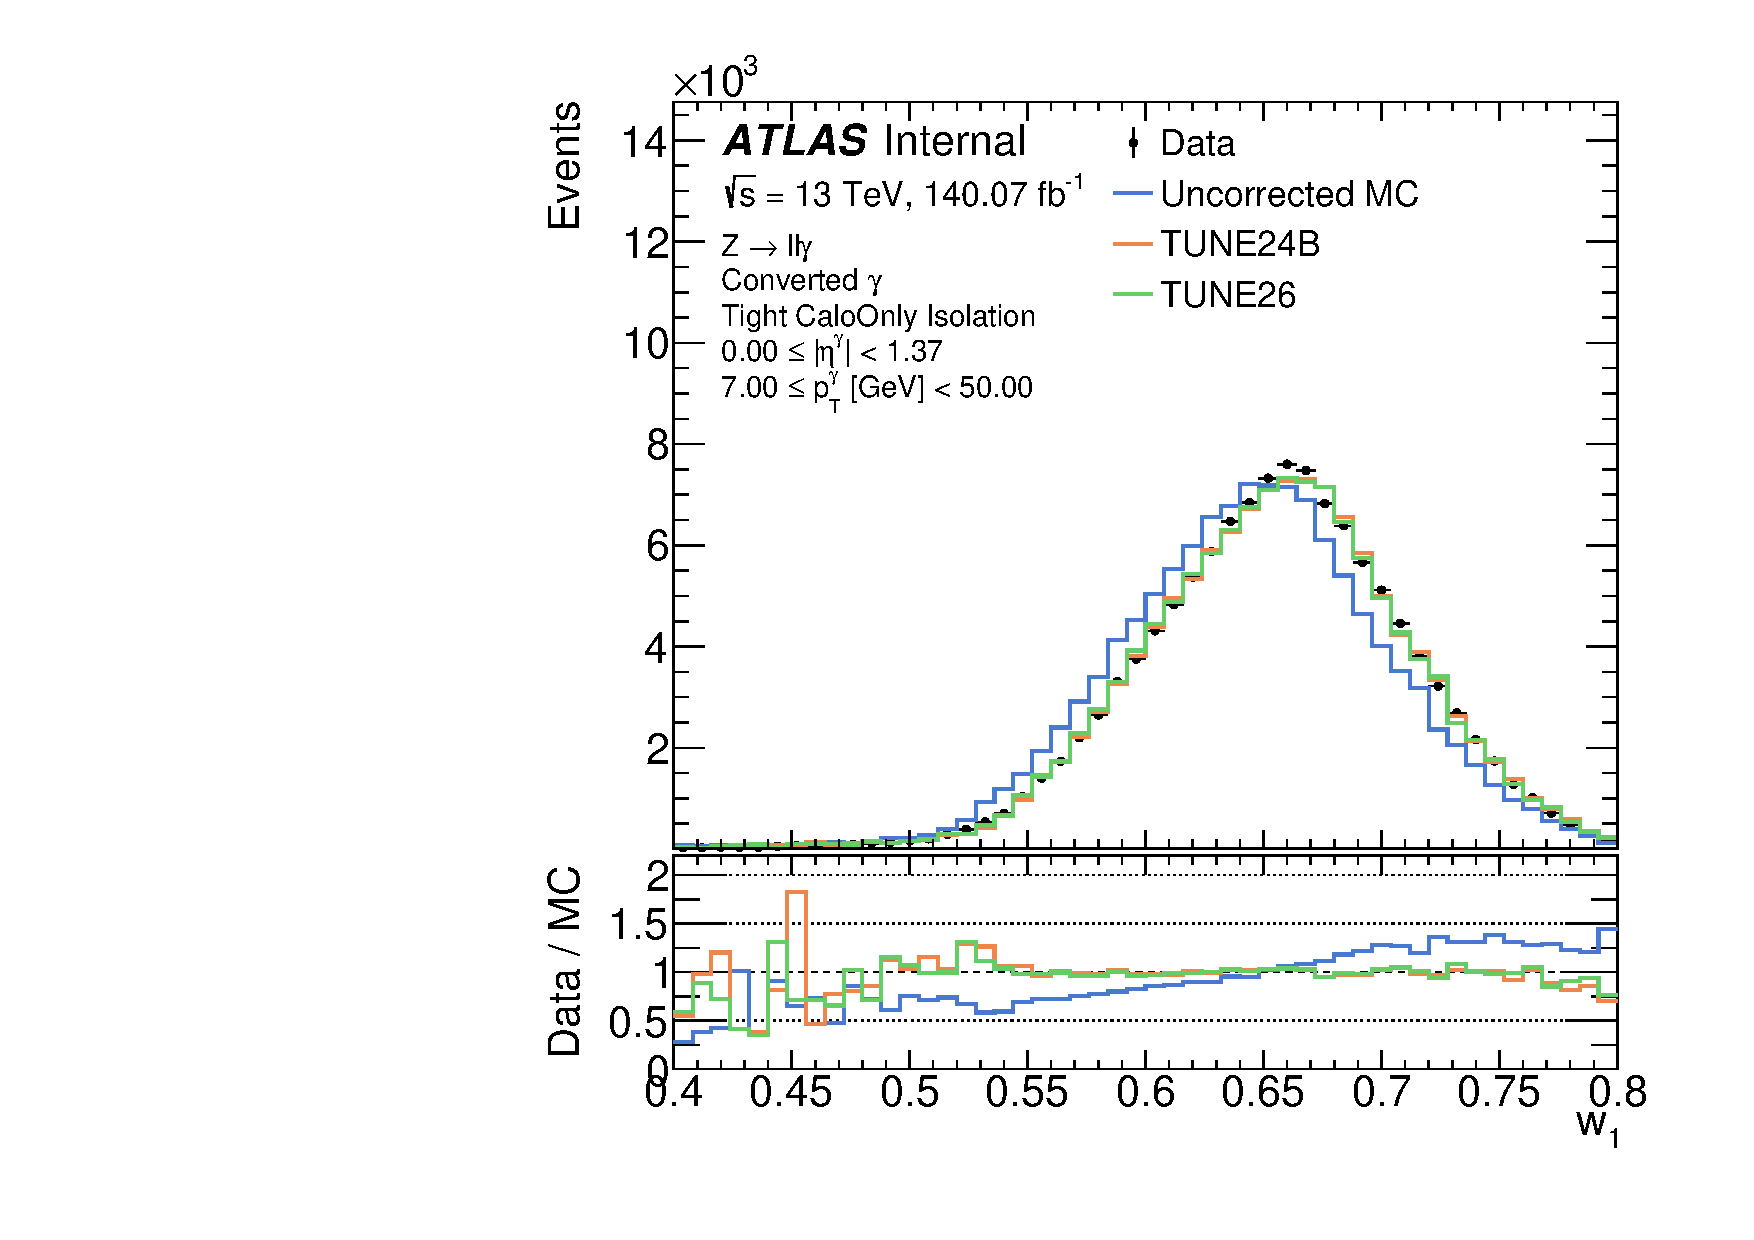
\includegraphics[width=\linewidth]{4_photonid/ffs/results/RZ/corrections/c/ptFull/etaCoarse/can__correction__ph_w1__Isotightcaloonly_IdNone__c__ptFullpt07p0__etaCoarseeta0p00}
        \caption{\wone, barrel.}
    \end{subfigure}
    \hfill
    \begin{subfigure}[h]{0.32\linewidth}
        \centering
        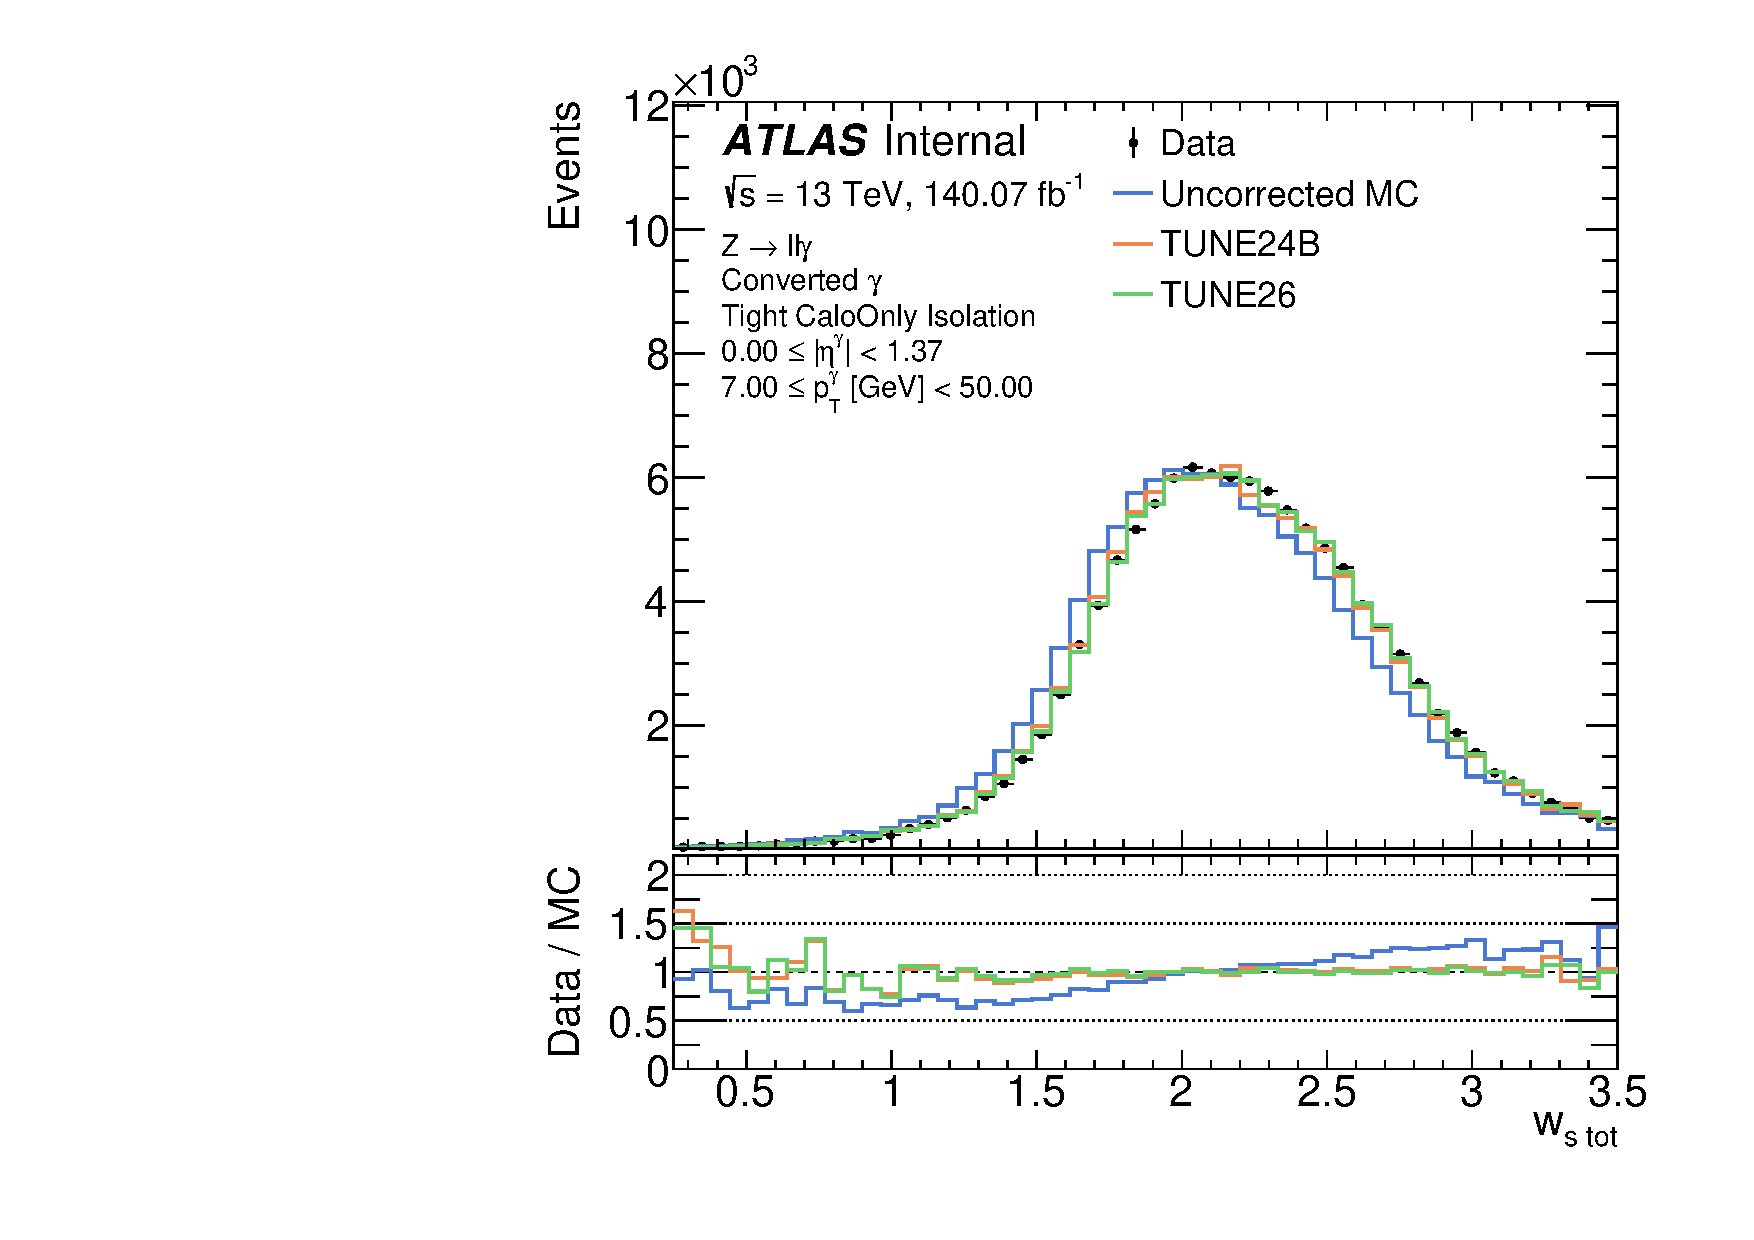
\includegraphics[width=\linewidth]{4_photonid/ffs/results/RZ/corrections/c/ptFull/etaCoarse/can__correction__ph_wstot__Isotightcaloonly_IdNone__c__ptFullpt07p0__etaCoarseeta0p00}
        \caption{\wstot, barrel.}
    \end{subfigure}\\
    \begin{subfigure}[h]{0.32\linewidth}
        \centering
        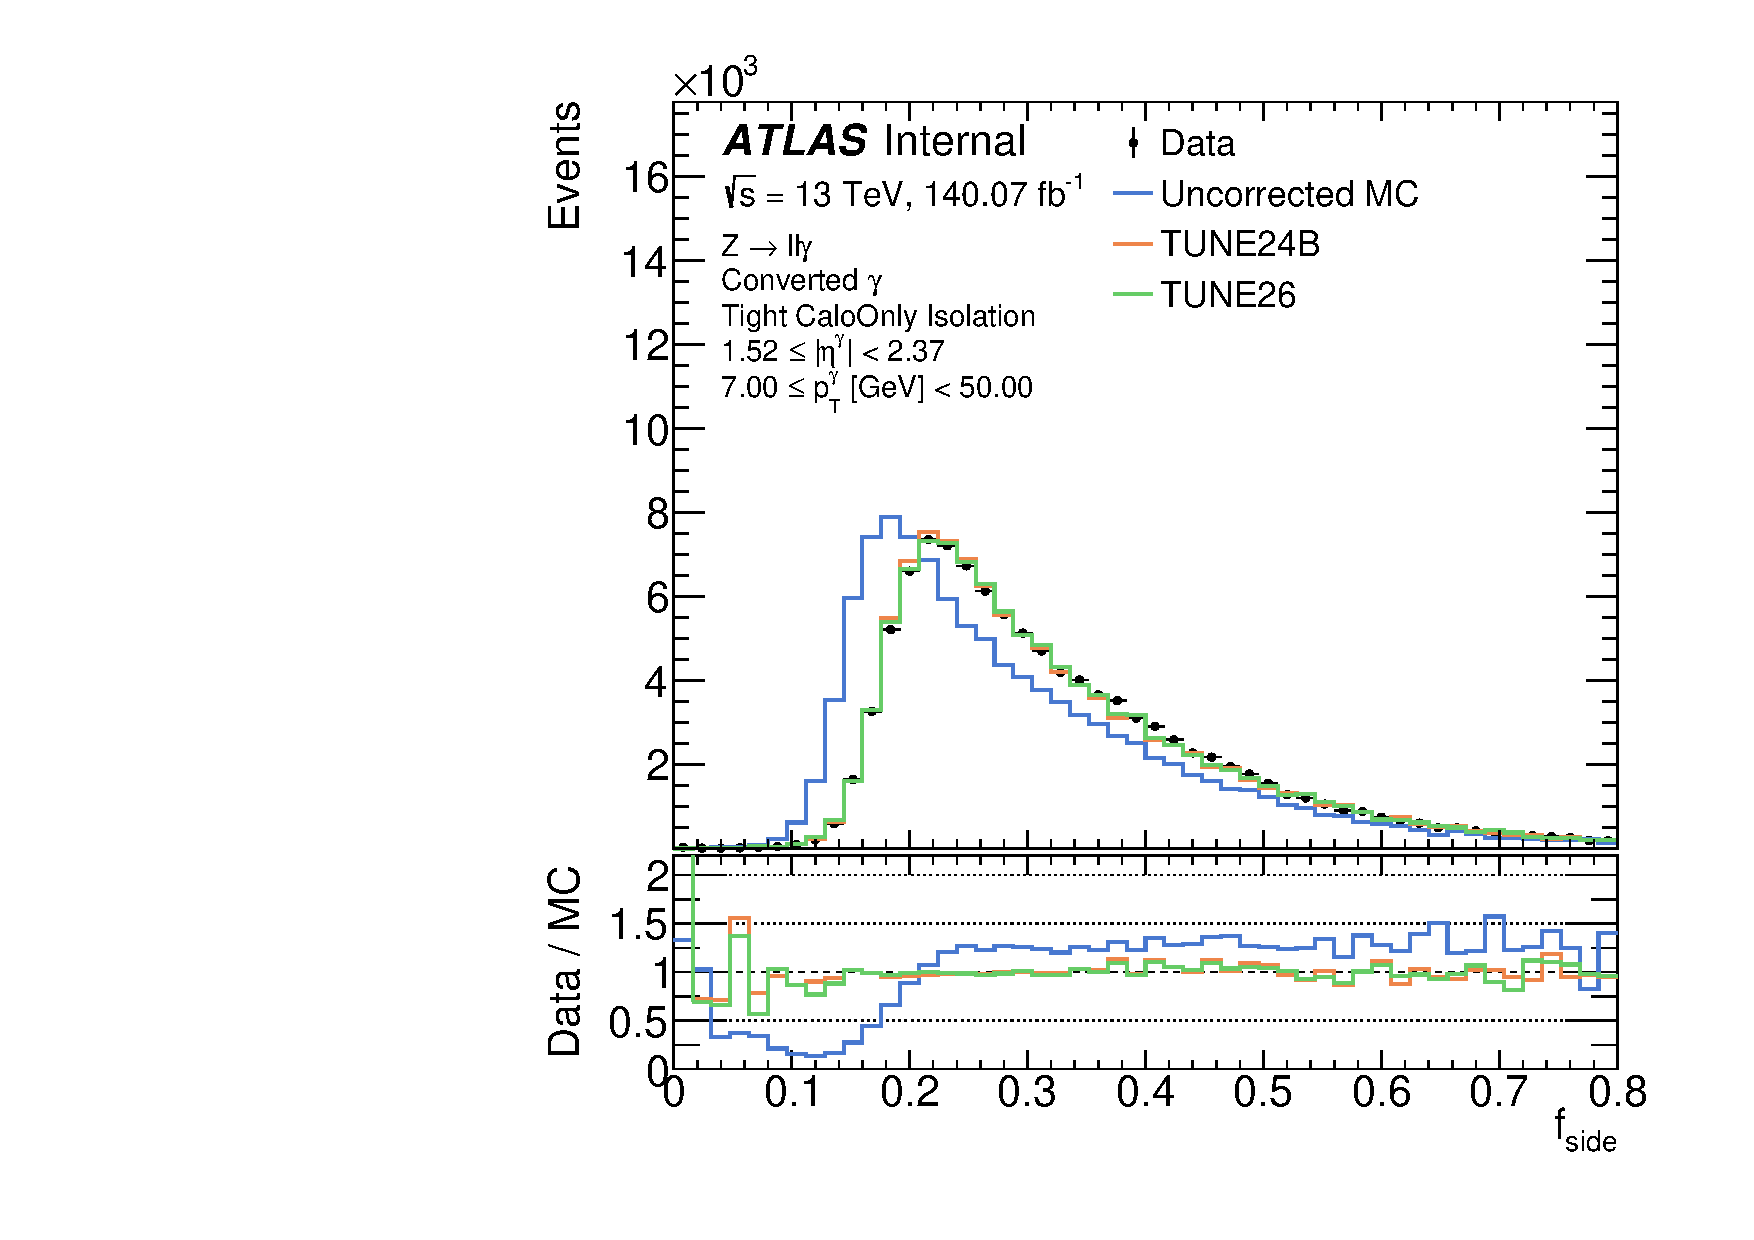
\includegraphics[width=\linewidth]{4_photonid/ffs/results/RZ/corrections/c/ptFull/etaCoarse/can__correction__ph_fside__Isotightcaloonly_IdNone__c__ptFullpt07p0__etaCoarseeta1p52}
        \caption{\fside, endcap.}
    \end{subfigure}
    \hfill
    \begin{subfigure}[h]{0.32\linewidth}
        \centering
        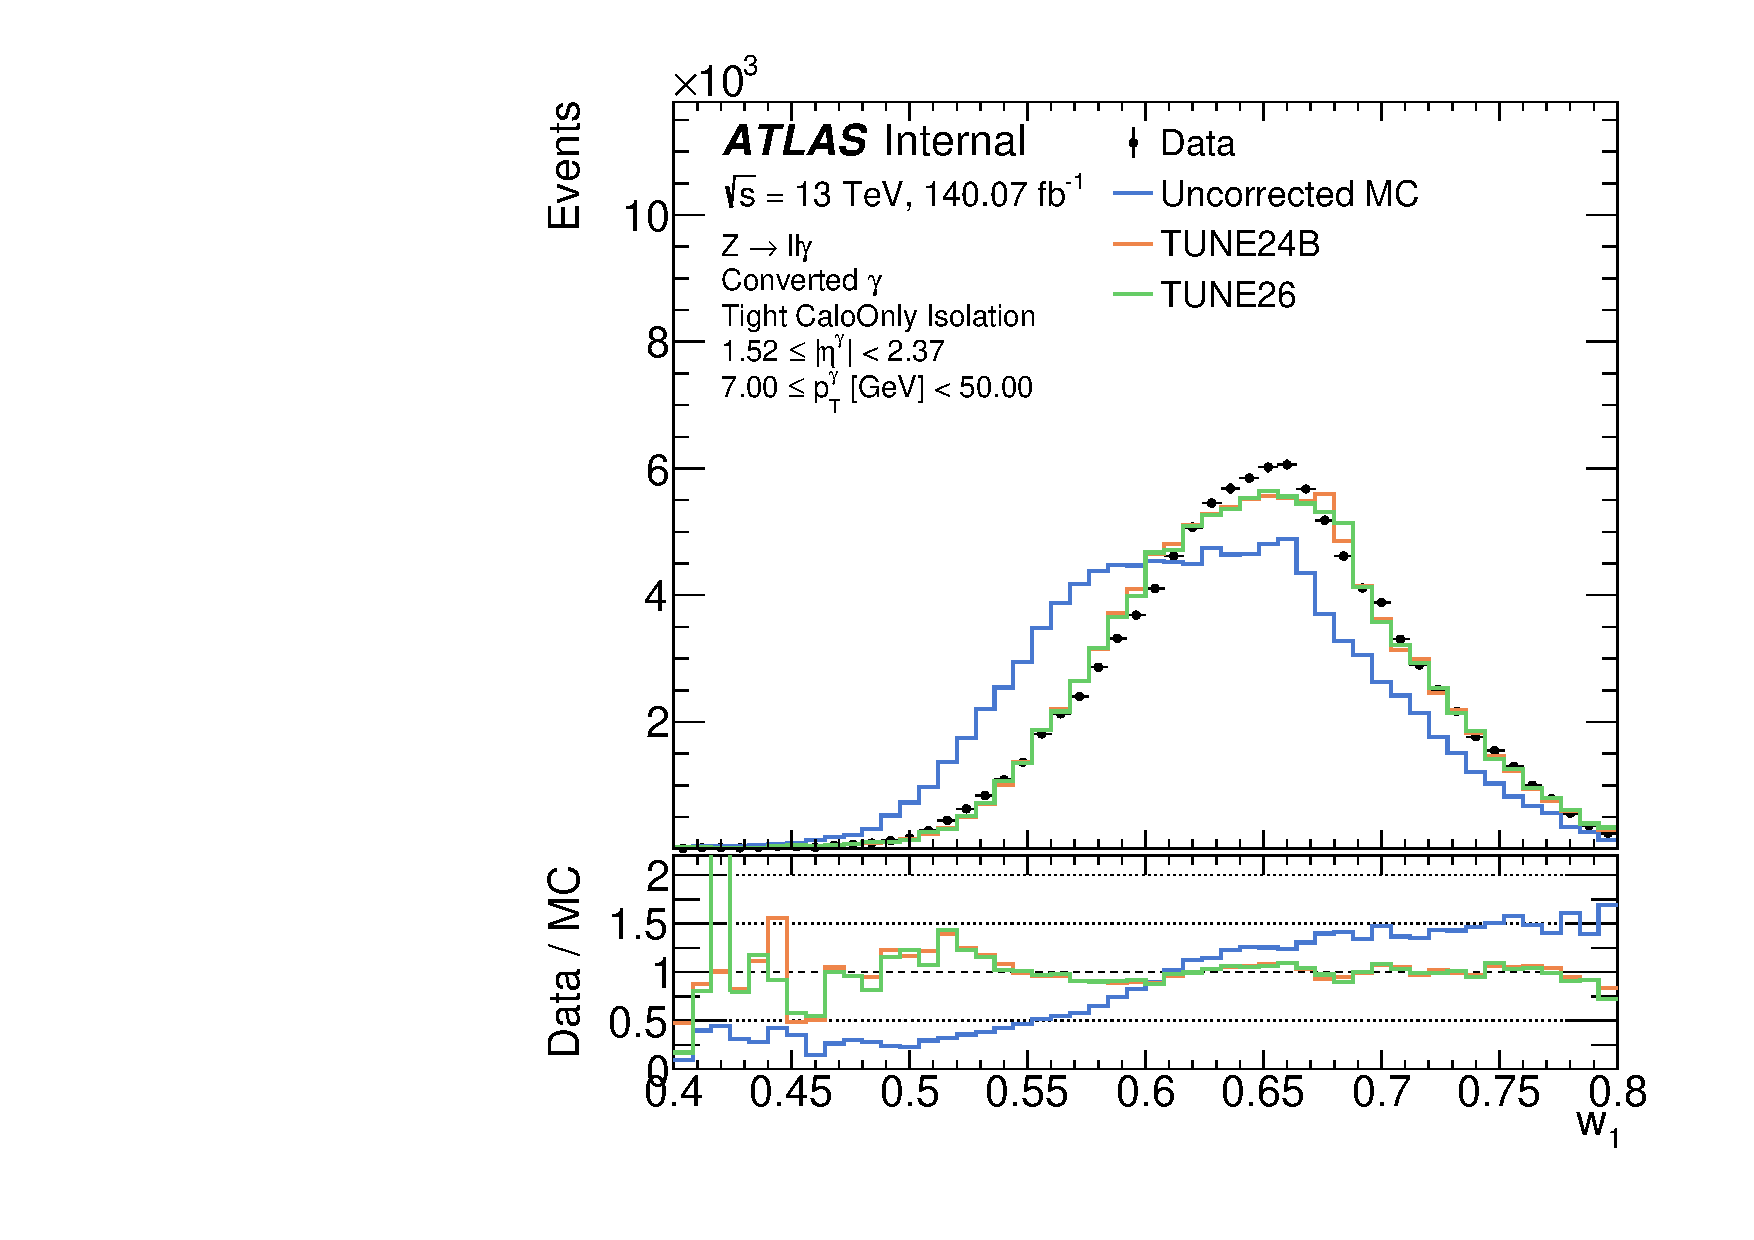
\includegraphics[width=\linewidth]{4_photonid/ffs/results/RZ/corrections/c/ptFull/etaCoarse/can__correction__ph_w1__Isotightcaloonly_IdNone__c__ptFullpt07p0__etaCoarseeta1p52}
        \caption{\wone, endcap.}
    \end{subfigure}
    \hfill
    \begin{subfigure}[h]{0.32\linewidth}
        \centering
        \includegraphics[width=\linewidth]{4_photonid/ffs/results/RZ/corrections/c/ptFull/etaCoarse/can__correction__ph_wstot__Isotightcaloonly_IdNone__c__ptFullpt07p0__etaCoarseeta1p52}
        \caption{\wstot, endcap.}
    \end{subfigure}\\
    \caption{Distribuciones de algunas \acp{SS} seleccionadas usando las muestras de \ac{RZ} para fotones convertidos luego de aplicar las correcciones de los \acp{FF} en la simulaci\'on. Las distribuciones de las \ac{SS} est\'an separadas para fotones en la regi\'on del barrel (fila de arriba) y en la regi\'on del endcap (fila de abajo). Los puntos negros representan los datos recolectados por \ac{ATLAS}, mientras que las simulaciones no corregidas y corregidas est\'an mostradas por las l\'ineas azules y verdes, respectivamente. Los paneles inferiores, en cada figura, muestra el cociente entre el histograma de datos con cada uno de los obtenidos de las simulaciones \ac{MC}.}
    \label{fig:ss_corrections:ffs:results:ss_rz}
\end{figure}

\begin{figure}[ht!]
    \centering
    \begin{subfigure}[h]{0.32\linewidth}
        \centering
        \includegraphics[width=\linewidth]{4_photonid/ffs/results/SP/corrections/c/ptFull/etaCoarse/can__correction__ph_fside__Isoloose_Idtight__c__ptFullpt0050p0__etaCoarseeta0p00}
        \caption{\fside, barrel.}
    \end{subfigure}
    \hfill
    \begin{subfigure}[h]{0.32\linewidth}
        \centering
        \includegraphics[width=\linewidth]{4_photonid/ffs/results/SP/corrections/c/ptFull/etaCoarse/can__correction__ph_w1__Isoloose_Idtight__c__ptFullpt0050p0__etaCoarseeta0p00}
        \caption{\wone, barrel.}
    \end{subfigure}
    \hfill
    \begin{subfigure}[h]{0.32\linewidth}
        \centering
        \includegraphics[width=\linewidth]{4_photonid/ffs/results/SP/corrections/c/ptFull/etaCoarse/can__correction__ph_wstot__Isoloose_Idtight__c__ptFullpt0050p0__etaCoarseeta0p00}
        \caption{\wstot, barrel.}
    \end{subfigure}\\
    \begin{subfigure}[h]{0.32\linewidth}
        \centering
        \includegraphics[width=\linewidth]{4_photonid/ffs/results/SP/corrections/c/ptFull/etaCoarse/can__correction__ph_fside__Isoloose_Idtight__c__ptFullpt0050p0__etaCoarseeta1p52}
        \caption{\fside, endcap.}
    \end{subfigure}
    \hfill
    \begin{subfigure}[h]{0.32\linewidth}
        \centering
        \includegraphics[width=\linewidth]{4_photonid/ffs/results/SP/corrections/c/ptFull/etaCoarse/can__correction__ph_w1__Isoloose_Idtight__c__ptFullpt0050p0__etaCoarseeta1p52}
        \caption{\wone, endcap.}
    \end{subfigure}
    \hfill
    \begin{subfigure}[h]{0.32\linewidth}
        \centering
        \includegraphics[width=\linewidth]{4_photonid/ffs/results/SP/corrections/c/ptFull/etaCoarse/can__correction__ph_wstot__Isoloose_Idtight__c__ptFullpt0050p0__etaCoarseeta1p52}
        \caption{\wstot, endcap.}
    \end{subfigure}\\
    \caption{\'Idem a la \Fig{\ref{fig:ss_corrections:ffs:results:ss_rz}} pero utilizando las muestras de \ac{SP}.}
    \label{fig:ss_corrections:ffs:results:ss_sp}
\end{figure}
























\section{Correcciones de energ\'ia de las celdas}
\label{sec:ss_corrections:cell_rw}

El diseño y la funcionalidad del \ac{ECAL} de \ac{ATLAS} se describi\'o en la \Sect{\ref{subsubsec:atlas:atlas:cals:ecal}}, así como el proceso a partir del cual los electrones y los fotones depositan sus energías en el \ac{ECAL}: creación de pares y radiación bremsstrahlung. Luego, a partir de estas deposiciones de energía en el \ac{ECAL} se construyen los \acp{SS} y se utilizan para la identificación de fotones. Sin embargo, el hecho de que las \acp{SS} calculadas mediante las simulaci\'on \ac{MC} y los datos \acp{SS} no coincidan, significa que las deposiciones de energía son diferentes entre estos dos, lo que lleva a un desacuerdo a un nivel inferior.

Aunque el método de \acf{FF} descripto anteriormente condujo a una excelente mejora del acuerdo entre los datos y las distribuciones \ac{MC}, sigue basándose en la modificación de variables de alto nivel y todas independientemente unas de otras. En cambio, otro enfoque diferente es el de corregir directamente los depósitos de energía de las celdas en la simulación \ac{MC}.
Esto permitir\'ia calcular todas las \acfp{SS} y cualquier otra variable que utiliza la energ\'ia de las celdas ya corregidas.

El enfoque de corregir las energ\'ias de las celdas del \ac{ECAL} se ha desarrollado y probado inicialmente para electrones~\cite{thesis_khandoga}, y posteriormente para fotones~\cite{thesis_belfkir}. Para el caso de los electrones, los resultados han sido muy prometedores, ya que se corrigieron sustancialmente las \acp{SS} de la segunda capa del calor\'imetro. Sin embargo, para los fotones, el mismo método que se utilizó para los electrones no funcion\'o de la forma que se esperaba, ya que sólo permiti\'o corregir las energ\'ias en promedio. Otro enfoque para corregir la simulación se basó en hacer coincidir eventos de datos y eventos simulados, estudio que s\'olo fue probado pseudodatos y resulta técnicamente complicado, pero que condujo a mejores resultados~\cite{thesis_belfkir}.

En la presente sección, se estudia una nueva forma de corregir las energías de celda en \ac{MC}, utilizando sólo la segunda capa del \ac{ECAL}, por simplicidad. El método comparte similitudes con el método \ac{FF}, lo que adem\'as facilita su comprensión.
En primer lugar, se presenta la selección de eventos especiales utilizada para este estudio. Se discute brevemente el m\'etodo de correcci\'on de energ\'ias utilizado por los primeros estudios basados en electrones y fotones, y luego se presenta en detalle cómo se mejora este método.





\subsection{Selecci\'on de eventos}
\label{subsec:ss_corrections:cell_rw:event_selection}

Los estudios presentados en esta sección se llevan a cabo con el mismo conjunto de datos utilizado para el cálculo \ac{FF}, descripto en la \Sect{\ref{subsec:ss_corrections:ffs:samples}}. Sin embargo, en este caso sólo se utilizan las muestras de \ac{RZ}.
Los eventos se seleccionan como se describe en la \Sect{\ref{subsec:pid_ss:pid:event_selection}}, utilizando fotones que pasan el criterio de aislamiento loose. Sin embargo, dado que estos estudios se basan en la información de la segunda capa del \ac{ECAL}, es necesario tener en cuenta una selección especial de las celdas que la conforman.

Cuando un electrón o fotón entra en el calorímetro, su huella en la segunda capa es un grupo visible de celdas que rodean a la más energética y central (también denominada \textit{hottest cell}). En este estudio, se consideran clusters de \(7\times 11\) celdas en \(\eta\times\phi\), mostradas en la \Fig{\ref{fig:ss_corrections:cell_rw:event_selection:cluster:arrangement}} donde tambi\'en se muestra la disposición utilizada.
Aproximadamente, el 90\% de la energía del cluster se reparte entre las 9 celdas centrales, resaltadas en azul en la \Fig{\ref{fig:ss_corrections:cell_rw:event_selection:cluster:arrangement}}. La energía media normalizada de los datos se muestra en la \Fig{\ref{fig:ss_corrections:cell_rw:event_selection:cluster:energy}}, visualizando cómo se distribuye la energía.

\begin{figure}[ht!]
    \centering
    \begin{subfigure}[t]{0.49\linewidth}
        \centering
        \includegraphics[width=0.5\linewidth]{4_photonid/cell_rw/cells_visualization}
        \caption{Disposici\'on de las celdas, mostrando para cada una su n\'umero. La celda central corresponde a la celda n\'umero 39 resaltada en azul oscuro, mientras que las 8 celdas vecinas se muestran resaltadas en celeste.}
        \label{fig:ss_corrections:cell_rw:event_selection:cluster:arrangement}
    \end{subfigure}
    \hfill
    \begin{subfigure}[t]{0.49\linewidth}
        \centering
        \includegraphics[width=0.8\linewidth]{4_photonid/cell_rw/cells-energy-u-etainclusive}
        \caption{Energ\'ia promedio en cada celda.}
        \label{fig:ss_corrections:cell_rw:event_selection:cluster:energy}
    \end{subfigure}
    \caption{Disposici\'on de las celdas y distribuci\'on de la energ\'ia entre las celdas del cluster.}
    \label{fig:ss_corrections:cell_rw:event_selection:cluster}
\end{figure}

En este trabajo, sólo se consideran los eventos en los que los clusters tienen el total de las 77 celdas. Además, se requiere en los eventos que la celda central sea la más energética.






\subsection{C\'alculo de las correcciones}
\label{subsec:ss_corrections:cell_rw:calculation}

\subsubsection{Primeros pasos}
\label{subsubsec:ss_corrections:cell_rw:calculation:previous}

Todos los eventos que superen la selección mencionada tendrán asociado un cluster, cada uno de los cuales tendrá \(N\) celdas y cada celda tendrá una energía \(E_i\), con \(i=1,\dots,N\). Para cada evento, en primer lugar, se obtiene la energía total del cluster \(E\) sumando las energ\'ias de cada una de las celdas \(E_i\).
El m\'etodo de las correcciones de las \acp{SS} mediante la correcci\'on de las energ\'ias depositadas en el \ac{ECAL} hace uso de las energ\'ias normalizadas en cada celda, \(e_i = E_i/E\). Estos valores dan a entender qu\'e proporci\'on de la energ\'ia total depositada tiene una celda en particular.

El proceso de correcci\'on comienza entonces calculando el valor medio de las distribuciones \(e_i\) (obtenidas una vez que todas los eventos pasan la selecci\'on) para la \(i\)-\'esima celda, en la simulaci\'on \ac{MC} y en los datos, y la diferencia entre estos valores dan lugar a la correcci\'on \(\Delta_i\) en dicha celda:
\begin{equation}
    \label{eq:ss_corrections:cell_rw:calculation:previous:old_corrections}
    \Delta_i = \overline{\left( \frac{ E_i^{\text{data}} }{ E^{\text{data}} } \right)} - \overline{\left( \frac{ E_i^{\text{MC}} }{ E^{\text{MC}} } \right)}
    = \bar e_i^{\text{data}} - \bar e_i^{\text{MC}}.
\end{equation}
Los valores \(E^{\text{data/MC}}\) son las energías totales del cluster para los datos y \ac{MC}, respectivamente.

La energ\'ia de la celda \(i\), se corrige entonces como
\begin{equation}
    \label{eq:ss_corrections:cell_rw:calculation:previous:correction_method}
    E_i^{\text{MC-RW}} = E_i^{\text{MC}} + \Delta_i E^{\text{MC}},
\end{equation}
que se traduce en desplazar la energía normalizada de la celda \(e_i^{\text{MC}}\) en una cantidad \(\Delta_i\), para que los valores medios de las distribuciones de \(e_i\) de datos y \ac{MC} coincidan. 

Tambi\'en es importante notar que, por definición, estos coeficientes de corrección suman 0 en todo el cluster:
\begin{equation*}
    \sum_i \Delta_i = \sum_i \overline{\left( \frac{ E_i^{\text{data}} }{ E^{\text{data}} } \right)} - \sum_i \overline{\left( \frac{ E_i^{\text{MC}} }{ E^{\text{MC}} } \right)}
    = \overline{\sum_i \frac{ E_i^{\text{data}} }{ E^{\text{data}} }} - \overline{\sum_i \frac{ E_i^{\text{MC}} }{ E^{\text{MC}} }}
    = 1 - 1 = 0,
\end{equation*}
implicando que el cambio de energ\'ia total del cluster se mantiene constante:
\begin{equation*}
    E^{\text{MC-RW}} \equiv \sum_i E_i^{\text{MC-RW}}
    = \sum_i E_i^{\text{MC}} + \sum_i \Delta_i E^{\text{MC}} = E^{\text{MC}} + E^{\text{MC}} \sum_i \Delta_i = E^{\text{MC}}.
\end{equation*}
Este hecho es de vital importancia, ya que no se desea cambiar la energ\'ia total del cluster en la simulaci\'on \ac{MC}, sino que se desea lograr una redistribuci\'on de la energ\'ia entre las celdas, de forma tal que cada una se asemeje a la de los datos.

Los coeficientes de correcci\'on resultantes para cada celda en clusters de 77 celdas, se pueden visualizar en la \Fig{\ref{fig:ss_corrections:cell_rw:calculation:previous:reweights}}. Como se puede notar de los valores mostrados, la celda central presenta una correcci\'on negativa, mientras que las 8 vecinas a la central tienen correcciones positivas. Esto se puede traducir a que en la simulaci\'on, la celda central suele tener m\'as energ\'ia, en promedio, que en los datos, mientras que lo opuesto ocurre en las vecinas. Mediante la aplicaci\'on de una correcci\'on negativa (implicando un corrimiento negativo de \(e_i\)), se remueve energ\'ia de la celda central que luego es distribu\'ida en las circundantes.

\begin{figure}[htbp]
    \centering
    \includegraphics[width=0.6\linewidth]{4_photonid/cell_rw/old_method/reweights_method1u_ptInclusive_eta040_phiInclusive}
    \caption{Correcciones a las energ\'ias de las celdas de la simulaci\'on \ac{MC} utilizando el mismo m\'etodo dise\~nado para electrones. \fixme{fix luminosity}}
    \label{fig:ss_corrections:cell_rw:calculation:previous:reweights}
\end{figure}

A partir de las energ\'ias de las celdas, se pueden calcular las \acp{SS} de la segunda capa del \ac{ECAL}, las cuales son \reta, \rphi y \weta:
\begin{gather*}
    \reta = \frac{E_{3\times 7}}{E_{7\times 7}}\\
    \rphi = \frac{E_{3\times 3}}{E_{7\times 3}}\\
    \weta = \sqrt{\frac{\sum_i E_i \eta^2_i}{\sum_i E_i} - \left( \frac{\sum_i E_i \eta_i}{\sum_i E_i} \right)^2}
\end{gather*}
donde \(E_{i\times j}\) es la energía de la celda sumada en una región de \(\eta\times\phi=i\times j\) celdas alrededor de la celda central. Se demostró en los estudios anteriores~\cite{thesis_belfkir} que este método sólo corrige las formas de las variables en promedio, pero las diferencias en la forma de permanecer. Esto se debe al hecho de que este método sólo corrige los valores medios de energ\'ia en las celdas. Sin embargo, estas distribuciones de energía siguen presentando diferencias, especialmente en lo que se refiere a las formas, lo que conduce a una situación muy similar a la observada para los \acp{FF}. De este modo, se puede emplear un enfoque muy similar para corregir los valores medios y los anchos de las distribuciones de energía normalizadas.
























\subsubsection{Nuevo m\'etodo de correcci\'on de energ\'ias}

Este nuevo método pretende corregir tanto el valor medio como la varianza de las distribuciones normalizadas de energía de las celdas, mediante la aplicaci\'on de corrimientos (shift) y estiramientos (stretch) de las mismas. De forma similar al enfoque seguido para las \acp{SS} utilizando el m\'etodo de \acp{FF}, una primera aproximación a los valores de shift y stretch de las distribuciones de energía consiste en calcular el valor medio y la raíz cuadrática media (RMS) de las mismas en cada celda, respectivamente.
Luego, la energía normalizada de la \(i\)-\'esima celda se obtiene como:
\begin{equation}
    \label{eq:ss_corrections:cell_rw:calculation:new:normalized_e}
    e_i^{\text{MC-RW}} =
    \underbrace{\frac{\text{RMS}_{e,i}^{\text{data}}}{\text{RMS}_{e,i}^{\text{MC}}}}_{\text{stretch}} e_i^{\text{MC}}
    +
    \underbrace{\left(\bar e_i^{\text{data}} - \frac{\text{RMS}_{e,i}^{\text{data}}}{\text{RMS}_{e,i}^{\text{MC}}} \bar e_i^{\text{MC}}  \right)}_{\text{shift}},
\end{equation}
donde el subíndice \(e\) en los valores de RMS indica que estos se calculan a partir de las distribuciones de energía normalizadas, y el \'indice \(i\) recorre todas las celdas del cluster. De la expresi\'on anterior se pueden identificar nuevamente un factor de shift, que es una transformaci\'on constante de la energ\'ia normalizada, y un factor de stretch, lineal en la variable que se requiere corregir.

Dado que la energía normalizada en la celda \(i\) puede calcularse como \(e_i^{j} = E_i^{j} / E^{j}\), para \(j=\)MC-RW, MC y datos, y se requiere tener la misma energía total del cluster luego de aplicar las correcciones (\(E^{\text{MC-RW}} = E^{\text{MC}}\)), se puede multiplicar la \Eqn{\ref{eq:ss_corrections:cell_rw:calculation:new:normalized_e}} por \(E^{\text{MC-RW}}\) y llegar a una expresión para \(E_i^{\text{MC-RW}}\):
\begin{equation}
    \label{eq:ss_corrections:cell_rw:calculation:new:correction_method}
    E_i^{\text{MC-RW}} =
    \frac{\text{RMS}_{e,i}^{\text{data}}}{\text{RMS}_{e,i}^{\text{MC}}} E_i^{\text{MC}}
    +
    \left( \bar e_i^{\text{data}} - \frac{\text{RMS}_{e,i}^{\text{data}}}{\text{RMS}_{e,i}^{\text{MC}}} \bar e_i^{\text{MC}} \right) E^{\text{MC}}.
\end{equation}
Por último, para garantizar que la energía del cluster permanezca constante, las energías de las celdas se reescalan por \(\sum_i E_i^{\text{MC}} / \sum_i E_i^{\text{MC-RW}}\).

Como el resultado de este procedimiento de correcci\'on de energ\'as involucra una correcci\'on de shift y otra de stretch, se obtienen dos matrices de correcci\'on, y un ejemplo de ellas se presenta en la \Fig{\ref{fig:ss_corrections:cell_rw:calculation:new:reweights}}.
En lo que sigue, este nuevo método se aplica para corregir las energías de las celdas, y se computa de forma inclusiva en \pt y \abseta, sólo separando entre fotones no convertidos y convertidos.

\begin{figure}[ht!]
    \centering
    \begin{subfigure}[h]{0.49\linewidth}
        \centering
        \includegraphics[width=\linewidth]{4_photonid/cell_rw/results/h_u_shift_mpl}
        \caption{Shift}
    \end{subfigure}
    \hfill
    \begin{subfigure}[h]{0.49\linewidth}
        \centering
        \includegraphics[width=\linewidth]{4_photonid/cell_rw/results/h_u_stretch_mpl}
        \caption{Stretch}
    \end{subfigure}
    \caption{Ejemplo de las matrices de correcci\'on de shift (izquierda) y stretch (derecha). Los valores mostrados corresponden al c\'alculo de las correcciones utilizando fotones no convertidos. Los valores de shift son multiplicados por un factor de 100 para mejorar su visualizaci\'on.}
    \label{fig:ss_corrections:cell_rw:calculation:new:reweights}
\end{figure}









\subsection{Resultados}
\label{subsec:ss_corrections:cell_rw:results}

La \Fig{\ref{fig:ss_corrections:cell_rw:calculation:new:reweights}} muestra las matrices de correcci\'on de shift y stretch obtenidas para fotones no convertidos. Puede observarse que, al igual que en el caso del m\'etodo anterior, la mayor corrección de shift se realiza en la celda central, donde el shift corresponde a un valor negativo. De la misma forma que en el caso anterior, los shifts de las celdas vecinas en la direcci\'on de \(\eta\) son positivos y grandes, indicando la redistribuci\'on de la energ\'ia de la celda central en estas dos vecinas.
Sin embargo, se puede notar que las segundas celdas vecinas en la direcci\'on de \(\phi\) sufren una gran correcci\'on, quitando energ\'ia mediante el shift, pero aumentando tambi\'en el ancho de la distribuci\'on, dado por los estiramientos positivos. Del resto de las celdas del cluster, se nota que no presentan corrimiento significativo, pero presenta un stretch \(<1\), indicando que se hacen m\'as angostas, especialmente las celdas de los extremos del cluster.

Utilizando estos factores de corrección para las energías normalizadas de cada celda, en las \Fig{\ref{fig:ss_corrections:cell_rw:results:cells}} se muestran las distribuciones de energía normalizadas resultantes para las celdas 28, 39 y 50~\footnote{Como fue mostrado en la \Fig{\ref{fig:ss_corrections:cell_rw:event_selection:cluster:arrangement}}, la celda número 39 es la central, mientras que las celdas 28 y 50 están a la izquierda y derecha, respectivamente, en la dirección \(\eta\).}. El nuevo método de correcci\'on consigue grandes mejoras en el acuerdo entre los datos y la simulaci\'on. Adem\'as, el m\'etodo logra corregir bien las colas de las distribuciones de todas las celdas, así como los picos de las mismas, lo que puede observarse especialmente en la celda 28.

\begin{figure}[ht!]
    \centering
    \begin{subfigure}[h]{0.32\linewidth}
        \centering
        \includegraphics[width=\linewidth]{4_photonid/cell_rw/results/cells/c__u__L2_e_cell_028_normTo1}
        \caption{Celda 28}
    \end{subfigure}
    \hfill
    \begin{subfigure}[h]{0.32\linewidth}
        \centering
        \includegraphics[width=\linewidth]{4_photonid/cell_rw/results/cells/c__u__L2_e_cell_039_normTo1}
        \caption{Celda 39}
    \end{subfigure}
    \hfill
    \begin{subfigure}[h]{0.32\linewidth}
        \centering
        \includegraphics[width=\linewidth]{4_photonid/cell_rw/results/cells/c__u__L2_e_cell_050_normTo1}
        \caption{Celda 50}
    \end{subfigure}
    \caption{Distribuciones de las energ\'ias normalizadas de las celdas 28, 39 y 50 de cluster de 77 celdas, para fotones no convertidos. Los puntos azules y rojos corresponden a las distribuciones de la simulaci\'on \ac{MC} con y sin las correcciones, respectivamente, mientras que el histograma gris representa los datos.}
    \label{fig:ss_corrections:cell_rw:results:cells}
\end{figure}



Para evaluar el comportamiento del nuevo procedimiento de correcci\'on aplicado a las \acp{SS} de la segunda capa \ac{ECAL}, en la \Fig{\ref{fig:ss_corrections:cell_rw:results:ss}} se muestra la comparación de los métodos de corrección para las variables \reta, \rphi y \weta. En los tres casos, se observa una mejora con respecto al \ac{MC} sin corregir, especialmente para \rphi y \weta. El método de correcci\'on de energía, en el caso de fotones no convertidos, no alcanza el nivel de acuerdo con los datos logrado por el m\'etodo de \acp{FF}, que ha demostrado proporcionar una excelente acuerdo con los datos experimentales. Sin embargo, casi no se observan diferencias entre el método de correcci\'on de energ\'ias y el de \acp{FF} para fotones convertidos, lo que indica que a\'un hay margen de mejora en las correcciones.


\begin{figure}[ht!]
    \centering
    \begin{subfigure}[h]{0.32\linewidth}
        \centering
        \includegraphics[width=\linewidth]{4_photonid/cell_rw/results/ss/c__u_eta00__ss_Reta}
        \caption{\reta, unconverted photons}
    \end{subfigure}
    \hfill
    \begin{subfigure}[h]{0.32\linewidth}
        \centering
        \includegraphics[width=\linewidth]{4_photonid/cell_rw/results/ss/c__u_eta00__ss_Rphi}
        \caption{\rphi, unconverted photons}
    \end{subfigure}
    \begin{subfigure}[h]{0.32\linewidth}
        \centering
        \includegraphics[width=\linewidth]{4_photonid/cell_rw/results/ss/c__u_eta00__ss_Weta2}
        \caption{\weta, unconverted photons}
    \end{subfigure}\\
    \begin{subfigure}[h]{0.32\linewidth}
        \centering
        \includegraphics[width=\linewidth]{4_photonid/cell_rw/results/ss/c__c_eta00__ss_Reta}
        \caption{\reta, converted photons}
    \end{subfigure}
    \hfill
    \begin{subfigure}[h]{0.32\linewidth}
        \centering
        \includegraphics[width=\linewidth]{4_photonid/cell_rw/results/ss/c__c_eta00__ss_Rphi}
        \caption{\rphi, converted photons}
    \end{subfigure}
    \begin{subfigure}[h]{0.32\linewidth}
        \centering
        \includegraphics[width=\linewidth]{4_photonid/cell_rw/results/ss/c__c_eta00__ss_Weta2}
        \caption{\weta, converted photons}
    \end{subfigure}\\
    \caption{Distribucioens de las \acp{SS} calculadas en la segunda capa del \ac{ECAL} para fotones no convertidos (fila superior) y convertidos (fila inferior) con pseudorapidez \(\abseta<0.6\), comparando los diferentes m\'etodos de correcci\'on con los datos. Los datos experimentales est\'an representados por los histogramas grises. La simulaci\'on \ac{MC} sin corregir se muestra con los puntos rojos, la simulaci\'on corregida por el m\'etodo de correcci\'on de energ\'ias con la l\'inea azul y la corregida por el m\'etodo de \acp{FF} con la l\'inea verde.}
    \label{fig:ss_corrections:cell_rw:results:ss}
\end{figure}






\section{Conclusiones y trabajo futuro}
\label{sec:ss_corrections:summary}

En el presente capítulo se han estudiado dos métodos para corregir el desacuerdo observado en las \acfp{SS} entre los datos y la simulación \ac{MC}.

El método de \acf{FF} se ha utilizado históricamente en la colaboración, al principio basado únicamente en simples desplazamientos de las distribuciones. A pesar de que las correcciones conducían a buenas mejoras y por tanto a la obtención de mejores \acp{SF}, seguían existiendo notables diferencias de forma entre los datos y la simulación. En el contexto de este trabajo, al añadir un término lineal a la transformación de la variable, se logra corregir los anchos de las distribuciones simuladas, lo que conduce a un acuerdo aún mejor con los datos. Este nuevo método de corrección de \acp{SS} mediante \acp{FF} se denomina método shift+stretch y actualmente se utiliza por toda la colaboración \ac{ATLAS}.

También se ha desarrollado un método novedoso y de menor nivel de correcci\'on que pretende modificar las energías en las celdas del \ac{ECAL}. Utilizando las distribuciones de energía en cada celda en clusters alrededor de la celda más energética, es posible corregir todas las \acp{SS} en simult\'aneo. Este método usa la misma estrategia de shift+stretch, pero esta vez aplicado a las distribuciones de energ\'ia normalizada en cada celda de la simulación \ac{MC}, para que coincida con la distribución encontrada en los datos. Aunque el método es nuevo y aún necesita de mejoras, como tambi\'en extenderlo a las dem\'as capas del \ac{ECAL}, ha dado resultados prometedores en los que algunas variables se corrigen de la misma manera que con el \acp{FF}. El método de correcci\'on de las energ\'ias de las celdas muestra un gran potencial en la colaboración, no sólo en el contexto de la identificación de fotones \textit{offline}, sino también a nivel de trigger.

\subsection{Trabajo a futuro}

Uno de los enfoques más interesantes y prometedores para corregir el \acp{SS} es el método basado en las correcciones de las energ\'ias de las celdas. Como se ha mencionado anteriormente, este enfoque podría emplearse en diferentes pasos del proceso de identificación de fotones, como en el nivel de trigger, o de forma \textit{offline} para corregir todos los \acp{SS} simultáneamente. Otro uso potencial e importante es utilizar los clusters corregidos para calcular directamente la identificación de fotones, por ejemplo, considerando a los clusters como imágenes y utilizando una red neuronal convolucional (CNN) para realizar la identificación de fotones~\cite{thesis_belfkir}.

Las \acfp{SS} tienen la gran ventaja de que se pueden interpretar fácilmente en términos físicos. Por esta razón, mantener estas variables sirve para comprender la física subyacente de los procesos. Seguir corrigiendo estas variables es de gran interés y hay varias formas de hacerlo. El método actual de transformar la variable pero utilizando términos de orden superior sigue siendo una tarea difícil, pero aún no explorada. Haciendo uso de las novedosas técnicas de Machine Learning (ML), es posible obtener factores de corrección para los términos de orden superior en la expansión, corrigiendo además los momentos de orden superior de las distribuciones (asimetría estad\'istica, curtosis, etc.). Otro enfoque interesante es el uso de un re-escaleo \acf{MV}, que se exploró en \Refn{\cite{thesis_spah}}, mostrando resultados muy prometedores.


\FloatBarrier
\part{B\'usqueda de Nueva Física en estados finales de fotón+jet de alta masa}
\label{part:search}
\chapter{Analysis motivation and strategy}
\label{ch:motivation_strategy}
\epigraph{\emph{“Champions keep playing until they get it right.”}}{Billie Jean King}

yet another template (yat)
\chapter{Modelos de señal y muestras simuladas}
\label{ch:samples}
\epigraph{\emph{``If you wish to make an apple pie from scratch, you must first invent the universe."}}{Carl Sagan}


La simulación de los distintos procesos físicos bajo consideración y de la respuesta del detector es necesaria para optimizar y estimar el rendimiento de los distintos análisis. Además permite desarrollar las estrategias para la identificación de partículas antes de la toma de datos y comprobar la eficiencia de los algoritmos. La preparación de búsquedas de nueva física requiere una simulación detallada del detector para estimar su potencial de descubrimiento y desarrollar métodos óptimos para medir las propiedades de las partículas. Una correcta comprensión de los eventos de señal y fondo es esencial para distinguir entre ambos. Una vez que se dispone de datos de colisiones reales, también se necesitan datos simulados para encontrar desviaciones de \ac{SM}. Todos los pasos de la simulación \ac{MC} se describieron en \Sect{\ref{sec:theory:mc_simulation}}.

De forma similar a cualquier análisis de física en el \ac{LHC}, este análisis hace uso de muestras simuladas, tanto para entender las posibles señales a descubrir, como para hacer un modelado correcto del fondo con estados finales de \gammajet.
En este capítulo se dan detalles sobre la generación y simulación de las muestras de señal y fondo.


\section{Señales}
\label{sec:samples:samples:sig}

\subsection{Quarks excitados}
\label{subsec:samples:samples:sig:qstar}

Una de las dos teorías que se ponen a prueba en esta tesis corresponde a la de \acf{EQ}, que se explicó detalladamente en la \Sect{\ref{subsec:theory:bsm:qstar}}. Si los quarks en realidad están compuestos por constituyentes más fundamentales unidos entre sí por alguna interacción desconocida, deberían aparecer nuevos efectos dependiendo del valor de la escala de composición \(\Lambda\).
También se vio que los \acp{EQ} se acoplan a los bosones del \ac{SM}, cuyas fuerzas están determinadas por las constantes de acoplamiento \(f\), \(f'\) y \(f_s\).

En esta teoría, hay un total de 5 parámetros: la escala de composición \(\Lambda\), los tres acoplamientos y la masa del \ac{EQ}. Para reducir el número de parámetros, es habitual fijar \(\Lambda = \mq\)~\cite{Zhan_Li_Liu_Li-2016}, y tomar las tres constantes de acoplamiento como iguales. De esta manera, sólo la masa y el acoplamiento son los parámetros libres de la teoría.

Se producen muestras de eventos de \ac{EQ} utilizando el software \pythia 8.245~\cite{Pythia8.2} con el conjunto de \acp{PDF1} a \ac{LO} de NNPDF 2.3~\cite{NNPDF2} y el tune A14 para el \ac{UE}.
Por primera vez en los estados finales de \gammajet en el \ac{LHC}, se consideran tres sabores diferentes: \ac{EQ} livianos (o light) \qstar (\(u^* / d^*\)) y pesados, separando entre \cstar y \bstar. Además, en este trabajo se estudian diferentes acoplamientos con los siguientes valores: \(f = 0.01, \, 0.1, \, 0.5, \, 0.75, \, 1.0\). Las masas de los \acp{EQ} y los acoplamientos utilizados se enumeran en la \Tab{\ref{tab:samples:samples:sig:qstar:xs}} donde se muestra la sección eficaz de los eventos multiplicada por el \textit{branching ratio}. Además, todos estos valores se muestran en la \Fig{\ref{tab:samples:samples:sig:qstar:xs}}.



\begin{table}[ht!]
    \centering
    \caption{Producto de la sección eficaz y el branching ratio en fb del modelo de \acp{EQ} para los tres sabores considerados y las distintas constantes de acomplamiento.}
    \resizebox{\linewidth}{!}{
        \begin{tabular}{lcccccc}
            \toprule
            \multirow{2}{*}{Quark excitado}  & \multirow{2}{*}{Masa [GeV]}  
            & \multicolumn{5}{c}{Acoplamiento \(f=f'=f_s\)}
            \\
            \cmidrule(l){3-7}
            &           & 0.01          & 0.10      & 0.50          & 0.75      & 1.00          \\
            \midrule
            \multirow{10}{*}{\(\qstar \rightarrow \gamma + u/d\)}
            & $500$     & 29.9400       & 3007.0000 & 75240.0000    & -         & 304200.0000   \\
            & $1000$    & 1.6560        & 165.0000  & 4153.0000     & -         & 16490.0000    \\
            & $2000$    & 0.0536        & 5.3800    & 133.2000      & -         & 520.8000      \\
            & $3000$    & -             & 0.4435    & 11.0200       & -         & 43.0600       \\
            & $4000$    & -             & 0.0488    & 1.2270        & -         & 4.8240        \\
            & $5000$    & -             & -         & 0.1450        & -         & 0.5877        \\
            & $5500$    & -             & -         & -             & -         & 0.2064        \\
            & $6000$    & -             & -         & 0.0163        & 0.0384    & 0.0719        \\
            & $6500$    & -             & -         & -             & -         & 0.0250        \\
            & $7000$    & -             & -         & -             & 0.0043    & 0.0088        \\
            \midrule
            \multirow{5}{*}{\(\cstar \rightarrow \gamma + c\)}
            & $500$     & 3.6540        & 362.2000  & 9051.0000     & -         & 36290.0000    \\
            & $1000$    & 0.1333        & 13.3400   & 332.4000      & -         & 1297.0000     \\
            & $2000$    & -             & 0.2434    & 6.0190        & -         & 23.6800       \\
            & $3000$    & -             & -         & 0.3135        & -         & 1.2450        \\
            & $4000$    & -             & -         & -             & -         & 0.0906        \\
            \midrule
            \multirow{5}{*}{\(\bstar \rightarrow \gamma + b\)}
            & $500$     & 0.6381        & 63.7700   & 1588.0000     & -         & 6324.0000     \\
            & $1000$    & 0.0220        & 2.2080    & 54.7600       & -         & 215.4000      \\
            & $2000$    & -             & 0.0372    & 0.9249        & -         & 3.6200        \\
            & $3000$    & -             & -         & 0.0446        & -         & 0.1770        \\
            & $4000$    & -             & -         & -             & -         & 0.0121        \\
            \bottomrule
        \end{tabular}
    }
    \label{tab:samples:samples:sig:qstar:xs}
\end{table}

\begin{figure}[ht!]
    \centering
    \includegraphics[width=0.6\linewidth]{5_resonances/samples/qstar_xs}
    \caption{Producto de la sección eficaz y el branching ratio de los diferentes modos de producción de los \acp{EQ} como función de la masa del \ac{EQ} a una energía de centro de masa de \(\sqs=13~\tev\). La figura muestra la comparación entre las señales de \qstar (azul), \cstar (naranja) y \bstar (verde) utilizando los acoplamientos de \(f=1.0,\, 0.75,\, 0.5\).}
    \label{fig:samples:samples:sig:qstar:xs}
\end{figure}


% Finalmente, en la \Fig{\ref{fig:samples:samples:sig:qstar:couplings}}, se muestra una comparación entre dos eñales de \qstar con diferentes acoplamientos.
% \begin{figure}[ht!]
%     \centering
%     \includegraphics[width=0.5\linewidth]{5_resonances/samples/qstar/couplings}
%     \caption{Comparación de dos señales de \qstar con masa \(\mq=5000~\gev\) utilizando diferentes acoplamientos: \(f=1.00\) (negro) y \(f=0.50\) (rojo).}
%     \label{fig:samples:samples:sig:qstar:couplings}
% \end{figure}




\subsection{Micro-Agujeros Negros}
\label{subsec:samples:samples:sig:qbh}

% La producción de \ac{QBH} en colisiones \pp del \ac{LHC} es predicha por modelos con dimensiones extra.

A través de la existencia de dimensiones extra, se predice la producción de \acf{QBH} en el \ac{LHC}, en colisiones \pp.
La sección eficaz de producción viene determinada por el radio gravitatorio que depende de la escala de Planck y del número de dimensiones, formulada como una sección eficaz clásica.


Las muestras de \ac{QBH} que decaen en un fotón y un partón se generan con el software \ac{QBH} 3.01 descripto en la \Refn{\cite{QBH}} y \pythia 8.3 para la hadronización y el \ac{UE}. Se ha utilizado el conjunto de \acp{PDF1} CTEQ6L1 junto con el tune estándar A14 del \ac{UE}. Para la generación de los eventos, se fija el rango de masa de producción de agujeros negros desde la escala de Planck \(m_p\) a \(3 m_p\) o la energía del centro de masa \sqs, la que sea menor y se consideran diferentes valores de \mth -- de ahora en más referida como \mqbh. Se tienen en cuenta dos modelos diferentes, en función del número de dimensiones adicionales \(n\). El modelo ADD, como se discute en la \Sect{\ref{subsec:theory:bsm:qbh}}, considera 6 dimensiones extra, lo que lleva a un número total de 10 dimensiones espacio-temporales. Por otro lado, el modelo RS1 propone sólo una dimensión extra deformada. Dado que para este análisis sólo interesa el estado final de \gammajet, se consideran los 6 estados no térmicos de agujero negro que se muestran en la \Sect{\ref{subsec:theory:bsm:qbh}}. Las secciones eficaces multiplicadas por el branching ratio de los dos modelos se representan en la \Fig{\ref{fig:samples:samples:sig:qbh:xs}} y los valores correspondientes en la \Tab{\ref{tab:samples:samples:sig:qbh:xs}}.


\begin{figure}[ht!]
    \centering
    \includegraphics[width=0.6\linewidth]{5_resonances/samples/qbh_xs}
    \caption{Producto de la sección eficaz y el branching ratio para los modelos RS1 (naranja) y ADD (azul) de \ac{QBH} para una energía de centro de masa de \(\sqs=13~\tev\).}
    \label{fig:samples:samples:sig:qbh:xs}
\end{figure}


\begin{table}[ht!]
    \caption{Suma de productos de sección eficaz y branching ratio en fb para los seis estados no termales de los \acp{QBH} que decaen en un par \gammajet.}
    \begin{center}
        \begin{tabular}{ccc}
            \toprule
            \mqbh [GeV] & ADD (\(n=6\))         & RS1 (\(n=1\)) \\
            \midrule
            1000        &                       & $2.69\times 10^{+4}$  \\
            2000        &                       & $4.17\times 10^{+2}$  \\
            3000        & $5.07\times 10^{+3}$  & $2.11\times 10^{+1}$  \\
            4000        & $3.88\times 10^{+2}$  & $1.60\times 10^{+0}$  \\
            5000        & $3.37\times 10^{+1}$  & $1.38\times 10^{-1}$  \\
            6000        & $2.90\times 10^{+0}$  & $1.18\times 10^{-2}$  \\
            7000        & $2.22\times 10^{-1}$  & $9.08\times 10^{-4}$  \\
            8000        & $1.35\times 10^{-2}$  &                       \\
            9000        & $5.64\times 10^{-4}$  &                       \\
            \bottomrule
        \end{tabular}
    \end{center}
    \label{tab:samples:samples:sig:qbh:xs}
\end{table}












\section{Fondos del SM}
\label{sec:samples:samples:bkg}


En el estado final de interés en el que hay al menos un fotón y un jet, la producción de fotones prompt de \ac{QCD} es el principal proceso del \ac{SM} que no puede reducirse.
Para estudiar esta particular contribución del fondo, se utilizan las muestras de \ac{MC}.
Además, existe una fracción considerable de eventos de dijet en los cuales un jet es mal-identificado como un fotón, teniendo entonces una contribución adicional al fondo. Para estudiar esta contribución en particular se ha utilizado un enfoque basado en datos que se describe en el \Ch{\ref{ch:bkg}}.


Se generan muestras con un gran número de eventos de \gammajet utilizando el software \Pythia 8.186~\cite{Pythia8.1}. Los procesos partónicos se simulan usando \ac{ME} a \ac{LO} con la inclusión de lluvias de partones de estado inicial y final, donde la parametrización de la estructura del protón viene dada por la \acp{PDF1} a \ac{LO} de \texttt{NNPDF2.3}~\cite{NNPDF2}.
El proceso de hadronización se modela mediante el modelo de cuerdas de Lund~\cite{Anderson-1983}, brevemente discutido en la \Sect{\ref{subsec:theory:mc_simulation:hadronisation}}, y la muestra también cuenta con una simulación del \ac{UE}.
Los parámetros del generador de eventos se ajustan según el tune A14 para \Pythia~\cite{Pythia-A14Tune}.
La muestra \pythia, dado que se genera a \ac{LO}, permite la separación entre las contribuciones de fotones directos y de fragmentación (véase la \Sect{\ref{subsec:theory:sm:prompt_photon}}).

Se consideran un conjuntos de muestras con diferentes umbrales de \pt a fin de optimizar la generación de los eventos. Los detalles de cada muestra, incluida la sección eficaz y las eficiencias de los filtros, se muestran en la \Tab{\ref{tab:samples:samples:bkg:samples}}.

\begin{table}[ht!]
    \caption{Detalles de las muestras simuladas del fondo de \gammajet.}
    \centering
    \resizebox{\textwidth}{!}{
        \begin{tabular}{l c l r r}
            \toprule
            Nombre de la muestra      &  Nombre del generador                  &   División de \pt [GeV]    & Sección eficaz [pb] &  Eficiencia del filtro  \\
            \midrule
            \gammajet direct &  \Pythia 8.244.3+\EvtGen v.1.7.0 &  \([70, 140]\)        & 28396.0           &  7.2863E-02   \\
            \gammajet direct &  \Pythia 8.244.3+\EvtGen v.1.7.0 &  \([140, 280]\)       & 2625.5            &  7.0598E-02   \\
            \gammajet direct &  \Pythia 8.244.3+\EvtGen v.1.7.0 &  \([280, 500]\)       & 198.39            &  6.0369E-02   \\
            \gammajet direct &  \Pythia 8.244.3+\EvtGen v.1.7.0 &  \([500, 800]\)       & 18.846            &  4.4596E-02   \\
            \gammajet direct &  \Pythia 8.244.3+\EvtGen v.1.7.0 &  \([800, 1000]\)      & 2.3312            &  2.4130E-02   \\
            \gammajet direct &  \Pythia 8.244.3+\EvtGen v.1.7.0 &  \([1000, 1500]\)     & 0.79945           &  2.3667E-02   \\
            \gammajet direct &  \Pythia 8.244.3+\EvtGen v.1.7.0 &  \([1500, 2000]\)     & 0.055512          &  1.9632E-02   \\
            \gammajet direct &  \Pythia 8.244.3+\EvtGen v.1.7.0 &  \([2000, 2500]\)     & 0.0052361         &  1.6644E-02   \\
            \gammajet direct &  \Pythia 8.244.3+\EvtGen v.1.7.0 &  \([2500, 3000]\)     & 0.00052733        &  1.4446E-02   \\
            \gammajet direct &  \Pythia 8.244.3+\EvtGen v.1.7.0 &  \([3000, \infty]\)   & 4.8856e-05        &  1.4371E-02   \\
            \gammajet frag   &  \Pythia 8.244.3+\EvtGen v.1.7.0 &  \([70, 140]\)        & 106180000.0       &  1.9271E-05   \\
            \gammajet frag   &  \Pythia 8.244.3+\EvtGen v.1.7.0 &  \([140, 280]\)       & 6702000.0         &  2.0959E-05   \\
            \gammajet frag   &  \Pythia 8.244.3+\EvtGen v.1.7.0 &  \([280, 500]\)       & 344070.0          &  2.0507E-05   \\
            \gammajet frag   &  \Pythia 8.244.3+\EvtGen v.1.7.0 &  \([500, 800]\)       & 23711.0           &  1.6991E-05   \\
            \gammajet frag   &  \Pythia 8.244.3+\EvtGen v.1.7.0 &  \([800, 1000]\)      & 2284.6            &  1.0123E-05   \\
            \gammajet frag   &  \Pythia 8.244.3+\EvtGen v.1.7.0 &  \([1000, 1500]\)     & 701.22            &  1.0074E-05   \\
            \gammajet frag   &  \Pythia 8.244.3+\EvtGen v.1.7.0 &  \([1500, 2000]\)     & 70.086            &  5.0238E-06   \\
            \gammajet frag   &  \Pythia 8.244.3+\EvtGen v.1.7.0 &  \([2000, \infty]\)   & 11.548            &  2.4464E-06   \\
            \bottomrule
        \end{tabular}
    }
    \label{tab:samples:samples:bkg:samples}
\end{table}

Como se mencionó más arriba, el fondo de las muestras de datos finales se estima a partir de los propios datos utilizando diferentes formas funcionales. Las muestras simuladas del fondo, no obstante, son de gran utilidad para el proceso de optimización de las regiones de señal (\Ch{\ref{ch:evt_selection}}) así como para la selección de las formas funcionales que se ajustará a los datos, como se verá en la \Sect{\ref{sec:bkg:modeling}}.
\chapter{Selección de eventos y optimización de las regiones de señal}
\label{ch:evt_selection}
\epigraph{\emph{``I don't want to believe. I want to know.”}}{Carl Sagan}

El estado final fotón+jet en la región de alta masa invariante representa un escenario ideal para búsquedas de física \ac{BSM}, pero para ello es imprescindible tener un excelente conocimiento del fondo producido por los procesos del \ac{SM}.

En las búsquedas de resonancias es habitual diseñar regiones de señal que sean capaces de proporcionar un fondo suave pero también una señal limpia sobre él. En este capítulo se presenta la selección de eventos que conduce a las regiones de señal utilizadas en este análisis.


\section{Trigger}
\label{sec:evt_selection:trigger}

Los eventos se recogen mediante un trigger de un sólo fotón (\texttt{HLT\_g140\_loose}) con un umbral de momento transverso de \(140~\gev\), que es el trigger de fotón sin preescalar de más bajo \pt para la mayor parte de los periodos de toma de datos\footnote{Para el año 2015, el trigger de más bajo \pt sin preescalar fue el \texttt{HLT\_g120\_loose}, pero el \texttt{HLT\_g140\_loose} también estaba en el menú}, seleccionando eventos con al menos un fotón que pasa el criterio de identificación \texttt{Loose}. Este trigger se ha mantenido sin escalar y es totalmente eficiente para fotones con \(>145~\gev\) con incertezas menores de \(0.1\%\) por encima de \(150~\gev\). Esta eficiencia se ha calculado con un método bootstrap siguiendo las prescripciones de la \Refn{\cite{ATLAS-PhotonTrigger-Performance-2015}} y se muestra en la \Fig{\ref{fig:evt_selection:trigger:trigger_perf_15_18}} en función de \(\ptgam\), \(\etagam\) y \(\avgmu\) para los diferentes años de toma de datos.

\begin{figure}[ht!]
    \centering
    \includegraphics[width=0.32\textwidth]{5_resonances/event_selection/trigger/perfPlots_2015-2018_thesis_DATA_Et_g140_loose}
    \includegraphics[width=0.32\textwidth]{5_resonances/event_selection/trigger/perfPlots_2015-2018_thesis_DATA_eta_g140_loose}
    \includegraphics[width=0.32\textwidth]{5_resonances/event_selection/trigger/perfPlots_2015-2018_thesis_DATA_avmu_g140_loose}
    \caption{Eficiencia del trigger \texttt{HLT\_g140\_loose} en función de \(\ptgam\) (izquierda), \(\etagam\) (centro) y \(\avgmu\) (derecha) medida utilizando datos de cada año entre 2015 y 2018.}
    \label{fig:evt_selection:trigger:trigger_perf_15_18}
\end{figure}








\section{Preselección}
\label{sec:evt_selection:presel}



Como se discute en la \Sect{\ref{sec:atlas:runs}}, durante un período de toma de datos, los eventos recolectados por el detector \ac{ATLAS} se agrupan en \acp{LB} para luego compilarlos en \acp{GRL}. Estas \acp{GRL} garantizan que los datos utilizados están libres de ineficiencias del detector o subdetectores, o en el haz del \ac{LHC}. Este análisis utiliza el conjunto completo de datos del Run-2 recolectados durante los años 2015 a 2018 a una energía de centro de masa de \(\sqs = 13~\tev\), correspondiendo a una luminosidad integrada de \(140.1 \pm 0.83~\ifb\) tras seleccionar los eventos de buena calidad de las \acp{GRL}. Además, se eliminan los eventos con distintos tipos de problemas, como aquellos con ruido del calorímetro o eventos corruptos, o aquellos con celdas del calorímetro que no funcionan.





\subsection{Objetos físicos}
\label{subsec:evt_selection:presel:objs}

En primer lugar se seleccionan los candidatos a fotones, leptones y jets con una serie de requisitos generales, denominados \textit{baseline}. Tras esta selección inicial, se aplica un procedimiento de eliminación de solapamientos (de ahora en más \textit{overlap removal}) para tratar el caso de que la misma partícula se reconstruya como objetos diferentes. Por último, los candidatos a fotones, leptones y jets utilizados para definir las distintas regiones de señal deben cumplir requisitos adicionales y en lo que sigue se denominarán objetos de \enquote{señal}.
% En los párrafos siguientes se brinda una breve descripción de los objetos utilizados en el análisis, basada en la descripción que figura en el \Ch{\ref{ch:objects}}.


\paragraph{Fotones}

Los candidatos a fotones deben pasar el criterio de identificación \texttt{Tight}, pasar un umbral de  \pt mayor que \(25~\GeV\) y estar contenidos en un rango de pseudorapidez de \(\abseta < 2.37\) descartando la región de transición barrel-endcap (\(1.37 < \abseta < 1.52\)). Se requiere un requisito adicional de \(\pt > 150~\GeV\) para los fotones de señal con el fin de garantizar que fue seleccionado por el trigger. También se requiere que el fotón esté aislado satisfaciendo los requisitos del \ac{WP} \texttt{Tight} (definido en la \Sect{\ref{subsec:objects:egamma:iso}}) que aplica cortes tanto en la energía de aislamiento calorimétrico como en el aislamiento de trazas, reduciendo así el fondo de jets mal identificados como fotones.


\paragraph{Electrones}

Los electrones baseline se seleccionan con \(\pt > 10~\gev\), \(\abseta < 2.47\) y se originan en el \ac{PV}. Se aplica el requisito de identificación \texttt{Loose}. Los electrones de señal se seleccionan además aplicando la identificación \texttt{Tight} y el requisito de aislamiento \texttt{Loose\_VarRad}, o \texttt{HighPtCaloOnly} si tienen \(\pt > 200~\gev\). Si luego de este proceso queda algún electrón, el evento se remueve completamente.


\paragraph{Muones}
Los muones baseline se seleccionan con la identificación \texttt{Medium}, tienen \(\pt > 10~\GeV\), \(\abseta < 2.7\) y son origiandos del \ac{PV}. Se requiere además que los muones de señal pasen el aislamiento \texttt{Loose\_VarRad} \ac{WP}. Se impone finalmente que el evento no tenga ningún muón.


\paragraph{Jets}

Los jets \ac{PFlow} se reconstruyen usando el algoritmo \antikt con \(R=0.4\) como se describe en la \Sect{\ref{sec:objects:jets}} y la selección baseline se define como aquellos que tienen \(\pt>20~\gev\) y \(\abseta<2.8\). El algoritmo \ac{NNJvt} se utiliza para eliminar los jets originados por interacciones de pileup para los jets con \(\pt<60~\gev\).

Los jets de sabor pesado son de gran importancia para este análisis ya que la búsqueda se realizará para tres sabores diferentes: jets light, \(c\), y \(b\). Por esta razón, se utiliza el novedoso tagger GN2, definido en la \Sect{\ref{sec:objects:ftag}}, para discriminar entre estos tres sabores.
El tagging de sabores sólo se aplica al jet de mayor \pt (denominado jet leading) y sólo si tiene \(\abseta < 2.5\).
También, como se mencionó en la \Sect{\ref{sec:objects:ftag}}, para discriminar entre los 3 se utiliza un proceso de taggeo bidimensional. En primer lugar, los jets se identifican como \bjets si pasan \ac{WP} de \(77\%\) de eficiencia.
En el segundo paso, los eventos en los que el jet leading no está taggeado como \bjet se identifican como \cjet si pasan el \ac{WP} de \(50\%\) de eficiencia. Los eventos que no superan ningunos de los dos \acp{WP} (\btag y \ctag) se definen como no taggeados o que contienen un jet light.


\subsection{Eliminación de objetos superpuestos}
\label{subsec:evt_selection:presel:or}

Debido a la identificación errónea de los objetos en su estado final, un único objeto podría reconstruirse como más de un objeto por lo que se contabilizaría varias veces. Para ello, se tiene en cuenta un procedimiento de eliminación de objetos superpuestos. La estrategia y el orden de eliminación se muestran en la \Tab{\ref{tab:evt_selection:presel:or}}. Dos tipos de objetos de referencia se comparan entre sí en función de su proximidad en términos de \DeltaR, así como de otros criterios. En cada paso, si se cumple el criterio de solapamiento resaltado en \textit{Condición}, el objeto que aparece en la columna \textit{Objeto a remover} se descarta, mientras que el \textit{Objeto con el que se compara} se mantiene en el evento. De esta forma se resuelven las ambigüedades en la reconstrucción del objeto y se evita el doble conteo de las señales del detector como dos tipos diferentes de objetos.

\begin{table}[ht!]
    \centering
    \caption{Pasos para la eliminación de objetos superpuestos.}
    \resizebox{\linewidth}{!}{
        \begin{tabular}{cccc}
            \toprule
            Paso    & Objeto a remover  & Objeto con el que se compara & Condición\\
            \midrule
            1       & muón              & electrón              & es un muón \ac{CT} y comparten trazas del \ac{ID}  \\
            2       & fotón            & electrón              & \(\DeltaR < 0.4\)                         \\
            3       & fotón            & muón                  & \(\DeltaR < 0.4\)                         \\
            4       & jet               & electrón              & \(\DeltaR < 0.2\)                         \\
            5       & electrón          & jet                   & \(\DeltaR < 0.4\)                         \\
            6       & jet               & muón                  & \(\DeltaR < 0.2\) and \(N_{\text{tracks}} < 3\) \\
            7       & muón              & jet                   & \(\DeltaR < 0.4\)\\
            8       & jet               & fotón                & \(\DeltaR < 0.4\)\\
            \bottomrule
        \end{tabular}
    }
    \label{tab:evt_selection:presel:or}
\end{table}










\section{Optimización de las regiones de señal}
\label{sec:evt_selection:sr_opt}

Las regiones de señal se definen teniendo en cuenta que el objetivo principal de la selección de eventos es conseguir:
\begin{itemize}
    \item Una distribución de fondo limpia y que decaiga suavemente, que contenga principalmente eventos \gammajet de fotones directos (\acs{DP}\acused{DP}) del canal \(s\) rechazando los eventos con fotones de fragmentación (\acs{FP}\acused{FP}), del canal \(t\) y de jets falseando fotones.
    \item Alta eficiencia y significancia de señal.
\end{itemize}


En primer lugar se realiza una serie de cortes básicos a partir de los cuales se basan todos los estudios de optimización.
\begin{itemize}
    \item Se requiere al menos un fotón \texttt{Tight} y aislado: \(\ngamma > 0\).
    \item Al menos un jet: \(\njets > 0\).
    \item En la interacción de dispersión dura para la producción de fotones prompt, el fotón y el jet llevan aproximadamente el mismo momento transverso. Por esta razón, se requiere que el jet tenga \(\ptjet > 150~\gev\).
    \item Se elimina cualquier jet que no sea el más energético y que tenga \(\ptjet < 60~\gev\).
    \item Se requiere la misma selección de pseudorapidez para el jet que para el fotón, para evitar fotones falseando jets: \(|\etajet| < 1.37\) o \(1.52 < |\etajet| < 2.37\).
    \item Para evitar la región del \textit{turn-on} de la distribución \myj, se requiere que \(\myj > 500~\gev\).
\end{itemize}
Para determinar la selección básica de eventos se realizan estudios sobre variables cinemáticas básicas optimizando en todos los casos para una alta significancia de la señal, que se presentan a continuación.


\subsection{Selecciones angulares del fotón y el jet}
\label{subsec:evt_selection:sr_opt:eta}



\subsubsection{Separación en la pseudorapidez}
\label{subsubsec:evt_selection:sr_opt:eta:deta}


La dinámica de los procesos en la dispersión dura \(2 \to 2\) puede investigarse utilizando la variable \(\theta^*\), donde \(\cos\theta^* \equiv \tanh \left(\Delta y / 2\right)\) y \(\Delta y\) es la diferencia entre la rapidez de las dos partículas en estado final. La variable \(\theta^*\) coincide con el ángulo de dispersión en el sistema de referencia del centro de masa y su distribución es sensible al spin de la partícula intercambiada. Para procesos dominados por el intercambio de gluones en el canal \(t\), como la producción de dijets en colisiones \pp y por tanto la producción de fotones de fragmentación, la sección eficaz diferencial se comporta como \(\left(1 - \left|\cos \theta^*\right|\right)^{-2}\) cuando \(\left|\cos \theta^*\right| \to 1\). En cambio, los procesos dominados por el intercambio de quarks en el canal \(t\), como la producción de \ac{DP} (véase la \Fig{\ref{fig:theory:sm:prompt_photon:feynman_lo_direct}}), se espera que tengan un comportamiento de la forma \(\left(1 - \left|\cos \theta^*\right|\right)^{-1}\) cuando \(\left|\cos \theta^*\right| \to 1\). Para ambos procesos también hay contribuciones del canal \(s\) que, sin embargo, no son singulares cuando \(\left|\cos \theta^*\right| \to 1\).
Este comportamiento en la sección eficaz se ha medido en la \Refn{\cite{ATLAS-IsolatedPhotonMeasurement}}.

Dado que el análisis considera jets altamente energéticos sumado al hecho de que los fotones no tienen masa, es posible aproximar \(\Delta\eta \sim \Delta y\).
% , y lograr separa a los eventos con \acp{DP}, de todos aquellos que no. Por esta razón, eliminando los eventos con altos valores de \detayj, se pueden eliminar los eventos con \acp{FP} y del canal \(t\).

\begin{figure}[ht!]
    \centering
    \begin{subfigure}[h]{0.49\linewidth}
        \centering
        \includegraphics[width=\linewidth]{5_resonances/event_selection/deta/can2d__direct__presel__phjet_m_phjet_deta}
        \caption{\acf{DP}.}
        \label{fig:evt_selection:sr_opt:eta:deta:2d:direct}
    \end{subfigure}
    \hfill
    \begin{subfigure}[h]{0.49\linewidth}
        \centering
        \includegraphics[width=\linewidth]{5_resonances/event_selection/deta/can2d__fragmentation__presel__phjet_m_phjet_deta}
        \caption{\acf{FP}.}
        \label{fig:evt_selection:sr_opt:eta:deta:2d:frag}
    \end{subfigure}
    \caption{Distribución bidimensional de \(\detayj-\myj\) para el fondo de \gammajet, separando entre \acp{DP} (izquierda) y \acp{FP} (derecha).}
    \label{fig:evt_selection:sr_opt:eta:deta:2d}
\end{figure}


La \Fig{\ref{fig:evt_selection:sr_opt:eta:deta:2d}} muestra la distribución bidimensional \Deta-\myj del fondo de \gammajet separando en eventos con \acp{DP} y \acp{FP}.
De estas distribuciones se desprende que hay una mayor concentración de eventos con valores más altos de \detayj para \acp{FP} que para \acp{DP}. Este escenario es cierto independientemente del valor de \myj pero es más prominente en la región de \(1 < \myj < 5~\tev\). Seleccionando eventos con \detayj bajo es posible rechazar una alta proporción de \acp{FP} y eventos del canal \(t\).

\begin{figure}[ht!]
    \centering
    \begin{subfigure}[h]{0.49\linewidth}
        \centering
        \includegraphics[width=\textwidth]{5_resonances/event_selection/deta/1d/preselM2000W/bkg_sig/1d/no_normalized/can__photonjet_Pythia_sig__preselM2000W__phjet_deta__wsignals_models__qStar_M2000__Run2__effrej}
        \caption{\(1000~\gev < \myj < 3000~\gev\)}
        \label{fig:evt_selection:sr_opt:eta:deta:1d:effrej_2000W}
    \end{subfigure}
    \hfill
    \begin{subfigure}[h]{0.49\linewidth}
        \centering
        \includegraphics[width=\textwidth]{5_resonances/event_selection/deta/1d/preselM6000W/bkg_sig/1d/no_normalized/can__photonjet_Pythia_sig__preselM6000W__phjet_deta__wsignals_models__qStar_M6000__Run2__effrej}
        \caption{\(5000~\gev < \myj < 7000~\gev\)}
        \label{fig:evt_selection:sr_opt:eta:deta:1d:effrej_6000W}
    \end{subfigure}\\
    \begin{subfigure}[h]{0.49\linewidth}
        \centering
        \includegraphics[width=\textwidth]{5_resonances/event_selection/deta/1d/preselM2000W/bkg_sig/1d/no_normalized/can__photonjet_Pythia_sig__preselM2000W__phjet_deta__wsignals_models__qStar_M2000__Run2__SB_significance}
        \caption{\(1000~\gev < \myj < 3000~\gev\)}
        \label{fig:evt_selection:sr_opt:eta:deta:1d:SB_2000W}
    \end{subfigure}
    \hfill
    \begin{subfigure}[h]{0.49\linewidth}
        \centering
        \includegraphics[width=\textwidth]{5_resonances/event_selection/deta/1d/preselM6000W/bkg_sig/1d/no_normalized/can__photonjet_Pythia_sig__preselM6000W__phjet_deta__wsignals_models__qStar_M6000__Run2__SB_significance}
        \caption{\(5000~\gev < \myj < 7000~\gev\)}
        \label{fig:evt_selection:sr_opt:eta:deta:1d:SB_6000W}
    \end{subfigure}
    \caption{Distribución de la variable \(\deta{\gamma}{j}\) en dos ventanas de \myj comparando le fondo con diferentes modelos de señal. El panel inferior de las \Figs{\ref{fig:evt_selection:sr_opt:eta:deta:1d:effrej_2000W}}{\ref{fig:evt_selection:sr_opt:eta:deta:1d:effrej_6000W}} muestran las eficiencias de las señales (líneas de colores), y el rechazo del fondo (histograma sombreado), si un corte del tipo \(\Deta < X\) es aplicado. Por otro lado, en las \Figs{\ref{fig:evt_selection:sr_opt:eta:deta:1d:SB_2000W}}{\ref{fig:evt_selection:sr_opt:eta:deta:1d:SB_6000W}}, los paneles inferiores muestran la significance de señal.}
    \label{fig:evt_selection:sr_opt:eta:deta:1d}
\end{figure}

Las comparaciones del fondo dominante obtenido con simulaciones con los modelos de señal utilizando esta variable se muestran en la \Fig{\ref{fig:evt_selection:sr_opt:eta:deta:1d}}. La selección en estas figuras corresponde a la selección de eventos con \(\mq - 1000 < \myj < \mq + 1000 ~\gev\), que consiste en una ventana de masa de \(2~\tev\) alrededor de la masa del modelo de señal.
El panel inferior en las \Figs{\ref{fig:evt_selection:sr_opt:eta:deta:1d:effrej_2000W}}{\ref{fig:evt_selection:sr_opt:eta:deta:1d:effrej_6000W}} muestra la eficiencia en las señales para las líneas coloreadas, mientras que el histograma sombreado muestra el rechazo de fondo si se aplica un corte del tipo \(\Deta < X\). De ellos se desprende que un corte de esta variable en \(\Deta \approx 1.6\) permitiría reducir considerablemente el fondo (\(\sim 80\%\)) manteniendo la mayoría de los eventos de señal (eficiencia \(60-80\%\)).
También se han llevado a cabo estudios que computan la significancia de este corte. Las \Figs{\ref{fig:evt_selection:sr_opt:eta:deta:1d:SB_2000W}}{\ref{fig:evt_selection:sr_opt:eta:deta:1d:SB_6000W}} muestran en los paneles inferiores la significancia de la señal para los mismos casos.
Exceptuando el corte trivial en \(\Deta = 0\), puede observarse que para valores altos de \myj puede alcanzarse la máxima significancia seleccionando eventos con \(\deta{\gamma}{j} \lesssim 1.6\), y por esta razón se ha optado por aplicar el corte \(\deta{\gamma}{j} < 1.6\) para el resto del análisis.
Otro aspecto importante que puede observarse en estas figuras es el hecho de que los eventos de fotones de fragmentación dominan en la región de alto \Deta, tal y como se preveía en la \Fig{\ref{fig:evt_selection:sr_opt:eta:deta:2d:frag}}. Aplicando este corte se logra entonces reducir en gran medida los eventos de \acp{FP}.


\subsubsection{Pseudorapidez del fotón y el jet}
\label{subsubsec:evt_selection:sr_opt:eta:etas}

En la región de baja masa \(\myj \lesssim 3~\tev\), se puede observar que hay una alta concentración de fondo con \(\etagam > 1.37\) y \(\etajet > 1.37\) en comparación con los modelos de señal, como se ve en la \Fig{\ref{fig:evt_selection:sr_opt:eta:etas:1d}}. Por este motivo, aplicando un corte en estas dos variables, la relación señal/fondo aumentaría sin afectar prácticamente la significancia de la señal ni en la eficiencia como se muestra en los paneles inferiores de las figuras. Por lo tanto, se decide eliminar los eventos con \(|\etagam| > 1.37\) y \(|\etajet| > 1.37\).

\begin{figure}[ht!]
    \centering
    \begin{subfigure}[h]{0.49\linewidth}
        \centering
        \includegraphics[width=\textwidth]{5_resonances/event_selection/eta/preselM2000W_deta/bkg_sig/1d/no_normalized/can__photonjet_Pythia_sig__preselM2000W_deta__absph_eta0__wsignals_models__qStar_M2000__Run2__SB_significance}
        \caption{\etagam}
        \label{fig:evt_selection:sr_opt:eta:etas:1d:ph}
    \end{subfigure}
    \hfill
    \begin{subfigure}[h]{0.49\linewidth}
        \centering
        \includegraphics[width=\textwidth]{5_resonances/event_selection/eta/preselM2000W_deta/bkg_sig/1d/no_normalized/can__photonjet_Pythia_sig__preselM2000W_deta__absjet_eta0__wsignals_models__qStar_M2000__Run2__SB_significance}
        \caption{\etajet}
        \label{fig:evt_selection:sr_opt:eta:etas:1d:jet}
    \end{subfigure}
    \caption{Distribuciones de \etagam y \etajet en una ventana de masa \(1000~\gev < \myj < 3000~\gev\) comparando las señales con el fondo de \yj. Los paneles inferiores muestran la significancia de la señal sobre el fondo.}
    \label{fig:evt_selection:sr_opt:eta:etas:1d}
\end{figure}



\subsection{Aislamiento extendido}
\label{subsec:evt_selection:sr_opt:extended_iso}

Los algoritmos de reconstrucción, identificación y aislamiento de fotones actúan para reducir los fondos instrumentales (hadrones mal identificados) a un nivel insignificante, pero parte del fondo (\acp{FP} y jets falseando fotones) permanece.
Para reducir aún más estos fondos, se investiga la contribución a la energía de aislamiento del fotón leading de los jets cercanos a él después de aplicar todas las selecciones mostradas anteriormente.

\begin{figure}[ht!]
    \centering
    \includegraphics[width=0.49\linewidth]{5_resonances/event_selection/extended_iso/can__photonjet_Pythia__presel_deta_etas__phjet_drmin__Run2}
    \caption{Distribución de \(\DeltaR_{\text{min}}\) para el fondo de \gammajet. Esta variable muestra la distancia mínima entre el fotón leading con el jet más cercano a el. El histograma rojo muestra la contribución de los eventos de \acp{DP}, mientras que el verde muestra la contribución de \acp{FP}.}
    \label{fig:evt_selection:sr_opt:extended_iso:phjet_drmin}
\end{figure}
% \begin{figure}[ht!]
%     \centering
%     \begin{subfigure}[t]{0.49\linewidth}
%         \centering
%         \includegraphics[width=\linewidth]{5_resonances/event_selection/extended_iso/can__photonjet_Pythia__presel_deta_etas__phjet_drmin__Run2}
%         \caption{Separación entre las contribuciones de fotones directos y de fragmentación.}
%         \label{fig:evt_selection:sr_opt:extended_iso:phjet_drmin:frag_direct}
%     \end{subfigure}
%     \hfill
%     \begin{subfigure}[t]{0.49\linewidth}
%         \centering
%         \includegraphics[width=\linewidth]{5_resonances/event_selection/extended_iso/can__photonjet_Pythia__phjet_drmin__regions_presel_deta_etas_J1_presel_deta_etas_J2_presel_deta_etas_J3_presel_deta_etas_J1_presel_deta_etas_J5__Run2}
%         \caption{Separación en la multiplicidad de los jets. El histograma con la línea roja muestra las contribuciones de los eventos en los que hay un sólo jet, la naranja donde hay dos, la verde donde hay 3 y la violeta donde hay más de 5.}
%         \label{fig:evt_selection:sr_opt:extended_iso:phjet_drmin:njets}
%     \end{subfigure}
%     \caption{Distribución de \(\DeltaR_{\text{min}}\) para el fondo de \gammajet. Esta variable muestra la distancia mínima entre el fotón leading con el jet más cercano a el.}
%     \label{fig:evt_selection:sr_opt:extended_iso:phjet_drmin}
% \end{figure}

En la \Fig{\ref{fig:evt_selection:sr_opt:extended_iso:phjet_drmin}} se muestra la distribución de \(\DeltaR_{\text{min}}\) separando entre eventos de \acp{DP} y \acp{FP}. Dicha variable mide la distancia angular entre el fotón leading y el jet más cercano. A partir de esta distribución es posible observar que la mayoría de los eventos muy cercanos al fotón (\(\DeltaR_{\text{min}}\) pequeño) son eventos de \acp{FP}.
% Además, se puede ver la contribución a dicha distribución separando los eventos con diferente multiplicidad de jets (\njet) mostrada en la \Fig{\ref{fig:evt_selection:sr_opt:extended_iso:phjet_drmin:njets}}. Se sabe que los eventos de fragmentación de fotones contienen más jets que los eventos procedentes de la producción directa de fotones, y a mayor multiplicidad de jets, mayores son las probabilidades de que un jet esté muy cerca del fotón, contribuyendo a la energía de aislamiento del mismo.


\begin{figure}[ht!]
    \centering
    \begin{subfigure}[t]{0.49\linewidth}
        \centering
        \includegraphics[width=\linewidth]{5_resonances/event_selection/extended_iso/can__photonjet_Pythia__phjet_drmin_ph_caloiso0__regions_presel_deta_etas__Run2}
        \caption{Contribución total de eventos de \acp{DP}+\acp{FP}.}
        \label{fig:evt_selection:sr_opt:extended_iso:phjet_drmin:etiso:full}
    \end{subfigure}
    \hfill
    \begin{subfigure}[t]{0.49\linewidth}
        \centering
        \includegraphics[width=\linewidth]{5_resonances/event_selection/extended_iso/can__photonjet_Pythia__phjet_drmin_ph_caloiso0__presel_deta_etas__Run2}
        \caption{Contribuciones de \acp{DP} y de \acp{FP} por separado.}
        \label{fig:evt_selection:sr_opt:extended_iso:phjet_drmin:etiso:separated}
    \end{subfigure}
    \caption{Distribución de la energía de aislamiento \(\etiso\) como función de \(\DeltaR_{\text{min}}\).}
    \label{fig:evt_selection:sr_opt:extended_iso:phjet_drmin:etiso}
\end{figure}

Para estudiar la contribución a la energía de aislamiento del fotón de estos jets se presenta la \Fig{\ref{fig:evt_selection:sr_opt:extended_iso:phjet_drmin:etiso:full}} con el valor medio de la energía de aislamiento del fotón en función de \(\DeltaR_{\text{min}}\). Los jets que se encuentran muy cerca del fotón contribuyen en gran medida a esta energía, especialmente los jets con \(\DeltaR (\gamma, j) < 1.0\), valor al que la energía comienza a aumentar drásticamente. Este comportamiento también se presenta por separado para la producción de \acp{DP} y de \acp{FP} en la \Fig{\ref{fig:evt_selection:sr_opt:extended_iso:phjet_drmin:etiso:separated}}, de los cuales la mayor contribución a la energía viene dada por los eventos de \acp{FP}.
En consecuencia, se considera un corte de esta variable en \(\DeltaR (\gamma, j) \geq 1.0\) para reducir los eventos de \acp{FP} y obtener una muestra de fotones más limpia.






\subsection{Momento transverso del jet}
\label{subsec:evt_selection:sr_opt:jet_pt}


Después de aplicar todos los cortes mencionados, una característica clave observada en los eventos de \acp{FP} es que hay una gran proporción de eventos en los que el jet leading lleva mucho más momento que el fotón leading. En una producción directa ideal de fotones, que es lo que se pretende con esta selección de eventos, tanto el fotón como el jet llevan aproximadamente el mismo \pt. Para estudiar si una selección basada en el jet y el fotón \pt es factible, se muestran las distribuciones \ptgam vs \ptjet en la \Fig{\ref{fig:evt_selection:sr_opt:jet_pt:ptgam_ptjet}} tanto para \acp{DP} como de \acp{FP}. De estas figuras se observa claramente que la producción de \acp{FP} es la que contribuye a tener eventos con \(\ptjet \gg \ptgam\).


\begin{figure}[ht!]
    \centering
    \begin{subfigure}[h]{0.49\linewidth}
        \centering
        \includegraphics[width=\linewidth]{5_resonances/event_selection/jet_pt/presel_deta_etas_iso/bkg/2d/can2d__direct__presel_deta_etas_iso__ph_pt0_jet_pt0}
        \caption{\acp{DP}.}
    \end{subfigure}
    \hfill
    \begin{subfigure}[h]{0.49\linewidth}
        \centering
        \includegraphics[width=\linewidth]{5_resonances/event_selection/jet_pt/presel_deta_etas_iso/bkg/2d/can2d__fragmentation__presel_deta_etas_iso__ph_pt0_jet_pt0}
        \caption{\acp{FP}.}
    \end{subfigure}
    \caption{Distribución bidimensional \ptgam-\ptjet para \acp{DP} y \acp{FP}.}
    \label{fig:evt_selection:sr_opt:jet_pt:ptgam_ptjet}
\end{figure}

\begin{figure}[ht!]
    \centering
    \begin{subfigure}[h]{0.49\linewidth}
        \centering
        \includegraphics[width=\linewidth]{5_resonances/event_selection/jet_pt/presel_deta_etas_iso_ptrel50/bkg/2d/can2d__direct__presel_deta_etas_iso_ptrel50__ph_pt0_jet_pt0}
        \caption{\acp{DP}.}
    \end{subfigure}
    \hfill
    \begin{subfigure}[h]{0.49\linewidth}
        \centering
        \includegraphics[width=\linewidth]{5_resonances/event_selection/jet_pt/presel_deta_etas_iso_ptrel50/bkg/2d/can2d__fragmentation__presel_deta_etas_iso_ptrel50__ph_pt0_jet_pt0}
        \caption{\acp{FP}.}
    \end{subfigure}
    \caption{Distribución bidimensional \ptgam-\ptjet para \acp{DP} y \acp{FP}, seleccionando eventos en los cuales el \pt del jet leading satisface \Eqn{\ref{eq:evt_selection:sr_opt:jet_pt:jet_pt_rel_X}} con \(X=0.5\).}
    \label{fig:evt_selection:sr_opt:jet_pt:ptgam_ptjet_X0.5}
\end{figure}



Para limpiar aún más la muestra de contribuciones de \acp{FP}, los eventos seleccionados deben satisfacer:
\begin{equation}
    \label{eq:evt_selection:sr_opt:jet_pt:jet_pt_rel_X}
    \frac{\ptjet - \ptgam}{\ptgam} < X, \qquad X \in [0, 1]
\end{equation}
donde \(X\) es la fracción de \ptgam permitida para el jet, definiendo así un valor superior de \ptjet para un \ptgam dado. El valor óptimo es \(X=0.5\), en el que la eficiencia de la señal es muy alta, mientras que el fondo rechazado consiste únicamente en eventos de \acp{FP}.

En la \Fig{\ref{fig:evt_selection:sr_opt:jet_pt:ptgam_ptjet_X0.5}} se muestra la distribución de fondo \ptgam vs \ptjet por separado para \acp{DP} y \acp{FP}, donde se observa que la gran mayoría de los eventos eliminados corresponden a \acp{FP}. La misma distribución para diferentes señales de \ac{EQ} se muestra en \Fig{\ref{fig:evt_selection:sr_opt:jet_pt:ptgam_ptjet_signals}} con eficiencias superiores al 95\%. La eficiencia de corte para el fondo y algunas señales \qstar se presenta en la \Tab{\ref{tab:evt_selection:sr_opt:jet_pt:efficiency_selection}}, donde se aprecia el poco efecto que tiene dicho corte en las señales.


\begin{figure}[ht!]
    \centering
    \begin{subfigure}[h]{0.32\linewidth}
        \centering
        \includegraphics[width=\linewidth]{5_resonances/event_selection/jet_pt/presel_deta_etas_iso/sig/2d/can2d__qStar_f1p00_M2000__presel_deta_etas_iso__ph_pt0_jet_pt0}
        \caption{\(\mq=2000~\gev\).}
    \end{subfigure}
    \hfill
    \begin{subfigure}[h]{0.32\linewidth}
        \centering
        \includegraphics[width=\linewidth]{5_resonances/event_selection/jet_pt/presel_deta_etas_iso/sig/2d/can2d__qStar_f1p00_M4000__presel_deta_etas_iso__ph_pt0_jet_pt0}
        \caption{\(\mq=4000~\gev\).}
    \end{subfigure}
    \hfill
    \begin{subfigure}[h]{0.32\linewidth}
        \centering
        \includegraphics[width=\linewidth]{5_resonances/event_selection/jet_pt/presel_deta_etas_iso/sig/2d/can2d__qStar_f1p00_M7000__presel_deta_etas_iso__ph_pt0_jet_pt0}
        \caption{\(\mq=7000~\gev\).}
    \end{subfigure}\\
    \begin{subfigure}[h]{0.32\linewidth}
        \centering
        \includegraphics[width=\linewidth]{5_resonances/event_selection/jet_pt/presel_deta_etas_iso_ptrel50/sig/2d/can2d__qStar_f1p00_M2000__presel_deta_etas_iso_ptrel50__ph_pt0_jet_pt0}
        \caption{\(\mq=2000~\gev\), con el corte de \ptjet aplicado.}
    \end{subfigure}
    \hfill
    \begin{subfigure}[h]{0.32\linewidth}
        \centering
        \includegraphics[width=\linewidth]{5_resonances/event_selection/jet_pt/presel_deta_etas_iso_ptrel50/sig/2d/can2d__qStar_f1p00_M4000__presel_deta_etas_iso_ptrel50__ph_pt0_jet_pt0}
        \caption{\(\mq=4000~\gev\), con el corte de \ptjet aplicado.}
    \end{subfigure}
    \hfill
    \begin{subfigure}[h]{0.32\linewidth}
        \centering
        \includegraphics[width=\linewidth]{5_resonances/event_selection/jet_pt/presel_deta_etas_iso_ptrel50/sig/2d/can2d__qStar_f1p00_M7000__presel_deta_etas_iso_ptrel50__ph_pt0_jet_pt0}
        \caption{\(\mq=7000~\gev\), con el corte de \ptjet aplicado.}
    \end{subfigure}\\
    \caption{Distribución bidimensional \ptgam-\ptjet para diferentes señales de \qstar con \(f=1.0\), seleccionando jets de acuerdo a la \Eqn{\ref{eq:evt_selection:sr_opt:jet_pt:jet_pt_rel_X}} con \(X=0.5\). Las primeras tres figuras muestran las distribuciones sin la aplicación del corte de \ptjet, mientras que las tres de abajo lo contienen.}
    \label{fig:evt_selection:sr_opt:jet_pt:ptgam_ptjet_signals}
\end{figure}



\begin{table}[ht!]
    \centering
    \caption{Eficiencias del corte en \ptjet del fondo y de distintas señales de \qstar.}
    \begin{tabular}{lc}
        \toprule
        & \(\varepsilon_{\text{rel}}\) \\
        \midrule
        \gammajet                      & $0.8827$ \\
        \(\mq=2000~\gev\),  \(f=1.00\) & $0.9707$ \\
        \(\mq=4000~\gev\),  \(f=1.00\) & $0.9918$ \\
        \(\mq=7000~\gev\),  \(f=1.00\) & $0.9942$ \\
        \bottomrule
    \end{tabular}
    \label{tab:evt_selection:sr_opt:jet_pt:efficiency_selection}
\end{table}



La variable más afectada por este corte es, como era de esperar, \ptjet. Esta distribución se muestra en la \Fig{\ref{fig:evt_selection:sr_opt:jet_pt:jet_pt}} antes y después de aplicar el corte. Se observa cómo la contribución de los eventos \acp{FP} disminuye drásticamente haciendo que la distribución \ptjet sea mucho más suave. Además, dado que el observable de interés es \myj, se presenta una comparación de esta distribución en la \Fig{\ref{fig:evt_selection:sr_opt:jet_pt:phjet_m}} para evaluar los cambios en el espectro. La aplicación de este corte particular sobre \ptjet tiene un efecto despreciable sobre la distribución final de \myj. Se observan diferencias muy pequeñas pero con un \myj muy bajo. Esto se debe a la asimetría en \pt que tenían el jet y el fotón (\(\ptjet \gg \ptgam\)).

En la selección final, se aplica el corte \((\ptjet - \ptgam) / \ptgam < 0.5\).

\begin{figure}[ht!]
    \centering
    \begin{subfigure}[h]{0.32\linewidth}
        \centering
        \includegraphics[width=\linewidth]{5_resonances/event_selection/jet_pt/presel_deta_etas_iso/bkg/1d/no_normalized/can__photonjet_Pythia__presel_deta_etas_iso__jet_pt0__Run2}
        \caption{Antes del corte en \ptjet.}
    \end{subfigure}
    \hfill
    \begin{subfigure}[h]{0.32\linewidth}
        \centering
        \includegraphics[width=\linewidth]{5_resonances/event_selection/jet_pt/presel_deta_etas_iso_ptrel50/bkg/1d/no_normalized/can__photonjet_Pythia__presel_deta_etas_iso_ptrel50__jet_pt0__Run2}
        \caption{Luego del corte en \ptjet.}
    \end{subfigure}
    \hfill
    \begin{subfigure}[h]{0.32\linewidth}
        \centering
        \includegraphics[width=\linewidth]{5_resonances/event_selection/jet_pt/can__photonjet_Pythia__jet_pt0__regions_presel_deta_etas_iso_presel_deta_etas_iso_ptrel50__Run2}
        \caption{Comparación final.}
    \end{subfigure}
    \caption{Distribución antes y después del corte en \ptjet para remover los eventos de \acp{FP}. Las contribuciones de \acp{DP} y de \acp{FP} se muestran por separado. En la figura de la derecha, la línea narnja (azul) representa la distribución luego (antes) de aplicar el corte en \ptjet.}
    \label{fig:evt_selection:sr_opt:jet_pt:jet_pt}
\end{figure}



\begin{figure}[ht!]
    \centering
    \includegraphics[width=0.45\linewidth]{5_resonances/event_selection/jet_pt/can__photonjet_Pythia__phjet_m__regions_presel_deta_etas_iso_presel_deta_etas_iso_ptrel50__Run2}
    \caption{Distribución de \myj antes y después del corte en \ptjet. La línea naranja (azul) representa la distribución antes (después) de la aplicación del corte.}
    \label{fig:evt_selection:sr_opt:jet_pt:phjet_m}
\end{figure}















\section{Regiones de señal}
\label{sec:evt_selection:sr}


Aplicando los cortes previamente definidos (resumidos en la \Tab{\ref{fig:evt_selection:sr:signal_regions_scheme}}) es posible obtener una distribución \myj limpia, en la que se eliminan la gran mayoría de \acp{FP} y eventos del canal \(t\) manteniendo una alta eficiencia de señal.

Para los objetivos de esta búsqueda, se clasifica al jet principal en tres posibles sabores: jets taggeados como light, \(c\) o \(b\). Haciendo uso del actual tagger de \ac{ATLAS} se pueden definir las regiones de señal SRB, SRC y SRL. En la \Fig{\ref{fig:evt_selection:sr:signal_regions_scheme}} se presenta un esquema de cómo se produce esta separación. En primer lugar, los \bjets se discriminan de light- y \cjets utilizando el \ac{WP} de \(77\%\) de eficiencia de \btagging. Al seleccionar aquellos jets que no consiguen entrar en la región SRB, se aplica el \ac{WP} de \ctagging de \(50\%\) de eficiencia para seleccionar \cjets y los que no pasan este \ctagger se clasifican como no etiquetados, o, simplemente \ljets.

\begin{table}[ht!]
    \caption{Definición de las regiones de señal.}
    \label{tab:evt_selection:sr:srs}
    \centering
    \begin{tabular}{|l|>{\centering\arraybackslash}p{0.08\linewidth}|>{\centering\arraybackslash}p{0.08\linewidth}|>{\centering\arraybackslash}p{0.08\linewidth}|>{\centering\arraybackslash}p{0.08\linewidth}|}
        \hline
        Cut                                     & SR & SRB & SRC & SRL \\
        \hline
        \ngamma                                 & \multicolumn{4}{c|}{$>0$} \\ \hline
        \ptgam [GeV]                            & \multicolumn{4}{c|}{$>150$} \\ \hline
        \njet                                   & \multicolumn{4}{c|}{$>0$} \\ \hline
        \ptjet [GeV]                            & \multicolumn{4}{c|}{$>150$} \\ \hline
        \etajet                                 & \multicolumn{4}{c|}{$<1.37 \,\,||\,\, (>1.52 \,\,\&\&\,\, <2.37)$} \\ \hline
        \myj [GeV]                              & \multicolumn{4}{c|}{$>500.$} \\ \hline
        \detayj                                 & \multicolumn{4}{c|}{$<1.6$} \\ \hline
        \etagam                                 & \multicolumn{4}{c|}{$<1.37$} \\ \hline
        \etajet                                 & \multicolumn{4}{c|}{$<1.37$} \\ \hline
        \(\Delta R_{\text{min}} (\gamma, j)\)   & \multicolumn{4}{c|}{$\geq 1.0$} \\ \hline
        \((\ptjet - \ptgam)/\ptgam\)            & \multicolumn{4}{c|}{$<0.5$} \\ \hline
        \btag \(77\%\)                          & - & Pasa   & \multicolumn{2}{c|}{Falla} \\ \hline
        \ctag \(50\%\)                          & - & -      & Pasa & Falla \\ \hline
    \end{tabular}
\end{table}

\begin{figure}[ht!]
    \centering
    \includegraphics[width=0.35\linewidth]{5_resonances/event_selection/SRL_SRC_SRB-crop}
    \caption{Esquema del taggeo de jets bidimensional.}
    \label{fig:evt_selection:sr:signal_regions_scheme}
\end{figure}
\chapter{Modelado de las señales e incertezas sistemáticas}
\label{ch:signals}


Esta búsqueda se centra en tres tipos diferentes de señales de resonancia \gammajet: \acp{EQ}, \acp{QBH} y resonancias genéricas de forma gaussiana. Para realizar los distintos tests de hipótesis así como los ajustes para la determinación de la forma funcional del fondo, deben conocerse sus espectros \myj esperados.
En este capítulo, estas formas de señal previstas se modelan mediante una \ac{PDF2} continua que posteriormente se incluye en los ajustes \ac{SB}.
También se estudian las incertezas sistemáticas teóricas y experimentales, ya que estas entran en los ajustes realizados de las funciones a los datos \'unicamente en las señales del análisis.













\section{Modelado de las señales}
\label{sec:signals:modeling}

Las señales son simuladas a partir de \ac{MC} para obtener tanto la forma de la masa invariante como sus eficiencias y aceptancias. Sin embargo, estas señales se generan en un conjunto limitado de masas (y acoplamientos en el caso de señales \acp{EQ}) pero, idealmente, se desea evaluar las predicciones de señal para todos los valores posibles de los parámetros.
Para lograr esta interpolación se sigue un procedimiento de dos pasos. En primer lugar, se transforman los histogramas en \acp{PDF2} utiizando el algoritmo \ac{KDE}. Este proceso de transformar un histograma en una \ac{PDF2} se empleó en el cálculo de los \acp{FF}, en la \Sect{\ref{subsec:ss_corrections:ffs:calculation}}, pero con el propósito de suavizar los histogramas.
% En este caso, el algoritmo \ac{KDE} se utiliza para recuperar una \ac{PDF2} a partir del histograma de la señal.


\begin{figure}[ht!]
    \centering
    \begin{subfigure}[h]{0.49\linewidth}
        \centering
        \includegraphics[width=\linewidth]{5_resonances/signal/can__kde_comparison_rhos__qStar_f1p00_M6500__SR}
        \caption{\qstar con \(\mq = 6500~\gev,\, f=1.0\)}
        \label{fig:signals:modeling:fine_factor_optimization_qstar}
    \end{subfigure}
    \begin{subfigure}[h]{0.49\linewidth}
        \centering
        \includegraphics[width=\linewidth]{5_resonances/signal/can__kde_comparison_rhos__cStar_f1p00_M1000__SR}
        \caption{\cstar con \(\mc = 1000~\gev,\, f=1.0\)}
        \label{fig:signals:modeling:fine_factor_optimization_cstar}
    \end{subfigure}
    \caption{Optimización de los fine-factors para señales de \acp{EQ} \qstar y \cstar. Los puntos representan la distribución original y las líneas de colores las distintas \acp{PDF2} estimadas con el m\'etodo \ac{KDE}.}
    \label{fig:signals:modeling:fine_factor_optimization}
\end{figure}

Este algoritmo necesita de fine-factors, que son optimizados uno a uno para cada una de las señales simuladas, tanto para el modelo \ac{EQ} como para los modelos \ac{QBH}. Se pueden encontrar ejemplos de la optimización en la \Fig{\ref{fig:signals:modeling:fine_factor_optimization}} para las señales de \qstar y \cstar. Lo más importante es lograr un modelado correcto en el \enquote{core} de la distribución, por lo que en algunos casos las colas no están perfectamente modeladas.

Una vez obtenidas todas las \acp{PDF2}, los modelos de señales para cualquier masa y/o acoplamiento intermedios se obtienen con un método de interpolación de momentos descripto en la \Refn{\cite{MomentMorphing}}. La interpolación se realiza de a pares: para obtener cualquier \ac{PDF2} intermedia, se utilizan las dos más cercanas al valor de masa/acoplamiento deseado. Por ejemplo, para obtener una señal interpolada con \(\mq = 3200~\gev\), las señales que se utilizan para la interpolación son las que tienen \(\mq = 3000~\gev\) y \(\mq = 4000~\gev\).
En la \Fig{\ref{fig:signals:modeling:final_interpolation}} se muestran las señales interpoladas con líneas discontinuas y las originales con líneas sólidas para el modelo \qstar. Para todas las señales interpoladas las formas conducen a una transición suave entre las muestras de señales originales.


\begin{figure}[ht!]
    \centering
    \includegraphics[width=0.6\linewidth]{5_resonances/signal/can__qstar__q_1p00__coupling_interpolation}
    \caption{Ilustración del m\'etodo de interpolación de momentos para la interpolación de las distribuciones de \myj de señale. Las \acp{PDF2} originales se muestran con las líneas de sólidas de distintos colores, mientras que todas las \acp{PDF2} interpoladas están representadas por las líneas discontinuas rojas.}
    \label{fig:signals:modeling:final_interpolation}
\end{figure}






















\section{Aceptancias y eficiencias}
\label{sec:signals:acc_eff}

La selección de eventos descripta en el capítulo anterior tiene por objetivo reducir todos los fondos que no sean del canal \(s\) de producción \gammajet, manteniendo una alta eficiencia de señal. Además, se utiliza el novedoso tagger GN2 para separar la región de señal inclusiva SR en tres ortogonales: SRB para \bjets, SRC para \cjets, y SRL para \ljets. Este es un aspecto crucial en el análisis ya que permite, por primera vez en el \ac{LHC}, estudiar resonancias de \ac{EQ} iniciadas por un \cstar, ortogonales a otros sabores.

\begin{table}[ht!]
    \centering
    \caption{Significancias de señales de \acp{EQ} sobre el fondo total en las regiones de señal SR, SRB, SRC y SRL. Las señales consideradas para cada sabor tienen un valor de la constante de acomplamiento de \(f=1.0\).}
    \begin{subtable}[t]{\linewidth}
        \centering
        \caption{\(m = 2000~\gev\) en una ventana de \(1000<\myj<3000~\gev\)}
        { \tiny
        \begin{tabular}{l >{\raggedleft\arraybackslash}p{0.18\linewidth}>{\raggedleft\arraybackslash}p{0.18\linewidth}>{\raggedleft\arraybackslash}p{0.18\linewidth}>{\raggedleft\arraybackslash}p{0.18\linewidth}}
                \toprule
                \textbf{Región de señal} & SR & SRB & SRC & SRL \\
                \midrule
                Fondo total & 89030.428 & 2570.406 & 14911.838 & 71548.184 \\
                \midrule
                jet \ra $\gamma$        & 3649.795 & 180.319 & 673.710 & 2795.767 \\
                $\gamma$ + jets \Pythia & 85380.633 & 2390.087 & 14238.128 & 68752.418 \\
                \midrule
                \bstar & 242.824, \(Z = 0.810\)    & 147.637, \(Z = 2.880\)  & 40.605, \(Z = 0.330\)    & 54.582, \(Z = 0.200\) \\
                \cstar & 1576.968, \(Z = 5.270\)   & 108.852, \(Z = 2.130\)  & 729.760, \(Z = 5.930\)   & 738.356, \(Z = 2.760\) \\
                \qstar & 31183.749, \(Z = 99.160\) & 625.209, \(Z = 11.880\) & 4335.836, \(Z = 33.970\) & 26222.705, \(Z = 92.810\) \\
                \bottomrule
            \end{tabular}
        }
    \end{subtable}\\
    \smallskip
    \begin{subtable}[t]{\linewidth}
        \centering
        \caption{\(m = 4000~\gev\) en una ventana de \(3000<\myj<5000~\gev\)}
        { \tiny
            \begin{tabular}{l >{\raggedleft\arraybackslash}p{0.18\linewidth}>{\raggedleft\arraybackslash}p{0.18\linewidth}>{\raggedleft\arraybackslash}p{0.18\linewidth}>{\raggedleft\arraybackslash}p{0.18\linewidth}}
                \toprule
                \textbf{Región de señal} & SR & SRB & SRC & SRL \\
                \midrule
                Fondo total & 200.888 & 5.999 & 27.677 & 167.212 \\
                \midrule
                jet \ra $\gamma$ fake   & 7.014 & 0.334 & 1.419 & 5.260 \\
                $\gamma$ + jets \Pythia & 193.874 & 5.665 & 26.258 & 161.951 \\
                \midrule
                \bstar & 0.708, \(Z = 0.050\) & 0.281, \(Z = 0.110\) & 0.136, \(Z = 0.030\) & 0.291, \(Z = 0.020\) \\
                \cstar & 5.514, \(Z = 0.390\) & 0.337, \(Z = 0.140\) & 1.668, \(Z = 0.310\) & 3.509, \(Z = 0.270\) \\
                \qstar & 295.673, \(Z = 17.530\) & 6.803, \(Z = 2.410\) & 33.739, \(Z = 5.520\) & 255.131, \(Z = 16.500\) \\
                \bottomrule
            \end{tabular}
        }
    \end{subtable}
    \label{tab:signals:acc_eff:qstar_signficances}
\end{table}


En la \Tab{\ref{tab:signals:acc_eff:qstar_signficances}}, se muestran el número de eventos para cada fondo considerado\footnote{El fondo de jets falseando fotones se estudia en el \Ch{\ref{ch:bkg}}.} y el número de eventos de señal en cada una de las SR, para dos señales de referencia. Las regiones de señal en las tablas, sin embargo, tienen un corte adicional en \myj de forma que sólo se cubre una ventana de \(2000~\gev\) alrededor de la señal hipotética. Por ejemplo, para señales con una masa hipotética de \(2000~\gev\), se seleccionan eventos con \(1000 \leq \myj \leq 3000~\gev\). Las señales mostradas corresponden a los tres tres sabores considerados. Para cada señal, como se puede apreciar, se muestra tambien la significancia de la misma según
\begin{equation}
    Z =
    \sqrt{
        2 \left(
            \left(s + b\right)
            \ln \left(1 + \frac{s}{b}\right)
            - s
        \right)
    }.
\end{equation}


En ambos casos, la señal de \qstar es la que presenta el mayor valor de significancia, independientemente de la región de señal. Esto es consecuencia de la mayor sección eficaz que tiene este proceso y, por este motivo, se utiliza la región SR inclusiva para buscar señales \qstar.
% \footnote{Un resumen general de todas las señales y regiones en las que se estudian se describe en \Sect{\ref{sec:bkg:modeling}}}.

Una característica importante a destacar es el marcado aumento de la sensibilidad de \bstar en la región dedicada SRB en comparación con la inclusiva. En el caso de \bstar con \(\mb=2000~\gev\), la significancia aumenta en un factor de \(3.5\). Esta mejora se debe al impresionante rendimiento del tagger GN2, que permite una gran separación de \bjets frente a otros sabores.

Con respecto a las señales de \cstar, la región SRC conduce también a un aumento de la significancia sobre el fondo, en comparación con la región inclusiva SR. Este es prominente a masas más bajas, donde el rendimiento del tagger GN2 es óptimo.
Sin embargo, dado que no se puede obtener una separación perfecta entre \cquarks y \lquarks con GN2, una cantidad no despreciable de eventos \cstar permanecen en la región \ltagged SRL. Con el fin de lograr una mayor sensibilidad para esta señal en particular, la búsqueda de las señales \cstar se lleva a cabo en tres regiones ortogonales simultáneamente, en lo que sigue denominadas SRC+SRB+SRL.


Las secciones eficaces de producción de señales se pueden transformar a la sección eficaz visible multiplicándolas por \(A \times \varepsilon\), donde \(A\) es la probabilidad de que el criterio de selección de eventos acepte el evento señal (\ac{EQ} o \ac{QBH} en este trabajo), referido como la \textit{aceptancia}, y \(\varepsilon\) es la eficiencia de reconstrucción e identificación. El factor \(A \times \varepsilon\) es de crucial interés también para la comunidad de altas energías, ya que permite comparar los resultados teóricos con los experimentales.

La aceptancia se calcula para cada señal como la relación
\begin{equation}
    A = \frac{N^{\text{truth}}_{\text{pass}}}{N_{\text{total}}}
\end{equation}
donde \(N_{\text{total}}\) es el número total de eventos generados y \(N^{\text{truth}}_{\text{pass}}\) es el número de eventos que superan los criterios de selección de eventos a nivel de partícula (es decir, toda la selección basada únicamente en cortes cinemáticos). Por otro lado, la eficiencia de selección se calcula como
\begin{equation}
    \varepsilon = \frac{N^{\text{reco/ID}}_{\text{pass}}}{N^{\text{truth}}_{\text{pass}}},
\end{equation}
y \(N^{\text{reco/ID}}_{\text{pass}}\) es el número de eventos que superan todos los requisitos de reconstrucción e identificación, como la identificación y aislamiento de fotones, la limpieza de jets y el trigger.


\begin{table}[ht!]
    \centering
    \caption{Medidas de aceptancias para las dos señales de referencia de \qstar con \(f = 1.0\). En la tabla, \(\varepsilon_{\text{abs}}\) hace referencia a la eficiencia absoluta de cada corte por separado, mmientras que \(\varepsilon_{\text{rel}}\) denota la eficiencia relativa de cada corte, es decir, la fracción de eventos que pasa un corte con respecto al n\'umero de eventos que pasó el corte anterior.}
    \resizebox{\columnwidth}{!}{
        \begin{tabular}{lrrrrrr}
            \toprule
                                                                    & \multicolumn{3}{c}{\(\mq=4000~\gev\)} & \multicolumn{3}{c}{\(\mb=4000~\gev\)} \\
            \midrule
            Corte                                                   & Eventos & $\varepsilon_{\text{abs}}$ & $\varepsilon_{\text{rel}}$ & Eventos & $\varepsilon_{\text{abs}}$ & $\varepsilon_{\text{rel}}$ \\
            \midrule
            Eventos totales                                         & 50000 & \multicolumn{2}{c}{1.0000}    & 50000 & \multicolumn{2}{c}{1.0000} \\
            $\ngamma>0$ y $\njets>0$ luego de sel. baseline         & 47702 & \multicolumn{2}{c}{0.9540}    & 47318 & \multicolumn{2}{c}{0.9464} \\
            $\ngamma>0$ y $\njets>0$ luego del OR                   & 47356 & 0.9471 & 0.9927               & 45304 & 0.9061 & 0.9574 \\
            $\ngamma>0$ y $\njets>0$ luego de sel. de objetos de señal & 45811 & 0.9162 & 0.9674               & 42505 & 0.8501 & 0.9382 \\
            Skim $\ngamma>0$                                        & 45811 & 0.9162 & 1.0000               & 42505 & 0.8501 & 1.0000 \\
            Skim $\ptgam > 145~\gev$                                & 45796 & 0.9159 & 0.9997               & 42500 & 0.8500 & 0.9999 \\
            Skim $|\etagam| < 1.37$ or ($1.52 < |\etagam| < 2.37$)  & 45796 & 0.9159 & 1.0000               & 42500 & 0.8500 & 1.0000 \\
            Skim $\njets>0$                                         & 45796 & 0.9159 & 1.0000               & 42500 & 0.8500 & 1.0000 \\
            Skim $\nlep=0$                                          & 44304 & 0.8861 & 0.9674               & 29659 & 0.5932 & 0.6979 \\
            $\ptgam > 150~\gev$                                     & 44304 & 0.8861 & 1.0000               & 29658 & 0.5932 & 1.0000 \\
            $\ptjet > 150~\gev$                                     & 43612 & 0.8722 & 0.9844               & 28504 & 0.5701 & 0.9611 \\
            $|\etajet| < 1.37$ o ($1.52 < |\etajet| < 2.37$)        & 41197 & 0.8239 & 0.9446               & 27362 & 0.5472 & 0.9599 \\
            $m_{\gamma j} > 500~\gev$                               & 41180 & 0.8236 & 0.9996               & 27291 & 0.5458 & 0.9974 \\
            $|\Delta\eta(\gamma,j)| < 1.6$                          & 30219 & 0.6044 & 0.7338               & 19821 & 0.3964 & 0.7263 \\
            $|\eta^{\gamma}| < 1.37$                                & 30056 & 0.6011 & 0.9946               & 19603 & 0.3921 & 0.9890 \\
            $|\etajet| < 1.37$                                      & 29880 & 0.5976 & 0.9941               & 19472 & 0.3894 & 0.9933 \\
            $\Delta R_{\text{min}}(\gamma,j) \geq 1.0$              & 27795 & 0.5559 & 0.9302               & 18073 & 0.3615 & 0.9282 \\
            $(\ptjet - \ptgam) / p_{T}^{\gamma} \leq 0.5$           & 27795 & 0.5559 & 1.0000               & 18073 & 0.3615 & 1.0000 \\
            \midrule
            Aceptancia                                              & \multicolumn{3}{c}{0.5559}            & \multicolumn{3}{c}{0.3615} \\
            \bottomrule
        \end{tabular}
    }
    \label{tab:signals:acc_eff:acceptances}
\end{table}

\begin{figure}[ht!]
    \centering
    \begin{subfigure}[h]{0.49\linewidth}
        \centering
        \includegraphics[width=\linewidth]{5_resonances/signal/acceptances/qstar/can__bStar__coupling_comparison__phjet_m_acceptance}
        \caption{\ac{EQ}}
        \label{fig:signals:acc_eff:acceptances:qstar}
    \end{subfigure}
    \hfill
    \begin{subfigure}[h]{0.49\linewidth}
        \centering
        \includegraphics[width=\linewidth]{5_resonances/signal/acceptances/QBH/can__QBH_n1__phjet_m_acceptance}
        \caption{\ac{QBH}}
        \label{fig:signals:acc_eff:acceptances:qbh}
    \end{subfigure}
    \caption{Aceptancias para las señales de \ac{EQ} (izquierda) y \ac{QBH} (derecha).}
    \label{fig:signals:acc_eff:acceptances}
\end{figure}

La \Tab{\ref{tab:signals:acc_eff:acceptances}} muestra la aceptancia medida para dos señales de \ac{EQ} de referencia con masa diferente, y se muestran todos los valores de aceptancia en la \Fig{\ref{fig:signals:acc_eff:acceptances:qstar}}, para cada sabor y con acoplamiento \(f=1\). Los mismos resultados para las señales de \ac{QBH} se presentan en la \Fig{\ref{fig:signals:acc_eff:acceptances:qbh}}.
Para las señales de \cstar y \bstar, puede observarse que se obtienen aceptancias más bajas en comparación con las señales de \qstar. La razón de este comportamiento se debe al veto leptónico que se realiza. Es probable que los quarks más pesados decaigan en quarks más livianos acompañados por un bosón \Wboson que decae en un par de leptones \(\ell \bar{\nu}\), o en un par de quarks que hadronizan, entonces lo más probable es que un leptón esté presente en el evento en este caso. En el caso de \qstar, sólo \(\sim 10\%\) de los eventos contienen un leptón, mientras que este número aumenta hasta casi \(\sim 30\%\) para la señal de \bstar, como se observa en la \Tab{\ref{tab:signals:acc_eff:acceptances}}.

Del mismo modo, en la \Fig{\ref{fig:signals:acc_eff:efficiencies}} y en la \Tab{\ref{tab:signals:acc_eff:efficiencies}}, se muestran las eficiencias de reconstrucción e identificación para los tres tipos de señales de \ac{EQ}. Como era de esperar, el mejor rendimiento se obtiene para las señales de \qstar cuando no se aplica ningun \ac{WP} de \ac{FTAG} (\(b\) o \ctagging). Además, se evidencia de las figuras una disminución significativa de la eficiencia en el rendimiento del tagger GN2 a altas masas y esto se refleja en las eficiencias medidas en las \Figs{\ref{fig:signals:acc_eff:efficiencies:cstar}}{\ref{fig:signals:acc_eff:efficiencies:bstar}}, donde para masas grandes la eficiencia del tagger disminuye hasta casi la mitad de su valor inicial.

\begin{figure}[ht!]
    \centering
    \begin{subfigure}[t]{0.32\linewidth}
        \centering
        \includegraphics[width=\linewidth]{5_resonances/signal/efficiencies/NS/sig/full_efficiencies/NOM/Nom/qstar/can__qStar__Nom__NS__efficiency}
        \caption{Señales de \qstar en la regón sin tagging..}
        \label{fig:signals:acc_eff:efficiencies:qstar}
    \end{subfigure}
    \hfill
    \begin{subfigure}[t]{0.32\linewidth}
        \centering
        \includegraphics[width=\linewidth]{5_resonances/signal/efficiencies/NSC50/sig/full_efficiencies/NOM/Nom/qstar/can__cStar__Nom__NSC50__efficiency}
        \caption{\cstar en la región con \ctagging.}
        \label{fig:signals:acc_eff:efficiencies:cstar}
    \end{subfigure}
    \hfill
    \begin{subfigure}[t]{0.32\linewidth}
        \centering
        \includegraphics[width=\linewidth]{5_resonances/signal/efficiencies/NSB/sig/full_efficiencies/NOM/Nom/qstar/can__bStar__Nom__NSB__efficiency}
        \caption{\bstar en la región con \btagging.}
        \label{fig:signals:acc_eff:efficiencies:bstar}
    \end{subfigure}
    \caption{Eficiencias de reconstrucción e identificación para las señales de \acp{EQ}.}
    \label{fig:signals:acc_eff:efficiencies}
\end{figure}


\begin{table}[ht!]
    \centering
    \caption{Eficiencias de reconstrucción e identificación para las señales de \acp{EQ} sin aplicar etiquetado de sabores, aplicando \btagging y aplicando \ctagging.}
    \resizebox{\columnwidth}{!}{
        \begin{tabular}{lrrrrrrrrr}
            \toprule
                                & \multicolumn{3}{c}{No FTAG, \(\mq=4.0~\TeV\)} & \multicolumn{3}{c}{\btag, \(\mb=4.0~\TeV\)} & \multicolumn{3}{c}{\ctag, \(\mc=4.0~\TeV\)} \\
            \midrule
            Corte               & Eventos & \(\varepsilon_{\text{abs}}\) & \(\varepsilon_{\text{rel}}\) &  Eventos & \(\varepsilon_{\text{abs}}\) & \(\varepsilon_{\text{rel}}\) & Eventos & \(\varepsilon_{\text{abs}}\) & \(\varepsilon_{\text{rel}}\) \\
            \midrule
            All                                      & $6.0000\times 10^{4}$ & \multicolumn{2}{r}{$1.0000$}  & $6.0000\times 10^{4}$ & \multicolumn{2}{r}{$1.0000$}  & $6.0000\times 10^{4}$ & \multicolumn{2}{r}{$1.0000$} \\
            GRL                                      & $6.0000\times 10^{4}$ & \multicolumn{2}{r}{$1.0000$}  & $6.0000\times 10^{4}$ & \multicolumn{2}{r}{$1.0000$}  & $6.0000\times 10^{4}$ & \multicolumn{2}{r}{$1.0000$} \\
            Cleaning                                 & $5.9841\times 10^{4}$ & \multicolumn{2}{r}{$0.9973$}  & $5.9819\times 10^{4}$ & \multicolumn{2}{r}{$0.9970$}  & $5.9808\times 10^{4}$ & \multicolumn{2}{r}{$0.9968$} \\
            Trigger                                  & $5.7381\times 10^{4}$ & $0.9564$ & $0.9589$           & $5.6861\times 10^{4}$ & $0.9477$ & $0.9506$           & $5.6961\times 10^{4}$ & $0.9494$ & $0.9524$ \\
            Good Vertex                              & $5.7381\times 10^{4}$ & $0.9564$ & $1.0000$           & $5.6861\times 10^{4}$ & $0.9477$ & $1.0000$           & $5.6961\times 10^{4}$ & $0.9494$ & $1.0000$ \\ 
            Bad Jet/Muon veto                        & $5.7380\times 10^{4}$ & $0.9563$ & $1.0000$           & $5.6859\times 10^{4}$ & $0.9476$ & $1.0000$           & $5.6961\times 10^{4}$ & $0.9494$ & $1.0000$ \\
            Skim                                     & $5.3414\times 10^{4}$ & $0.8902$ & $0.9309$           & $5.2514\times 10^{4}$ & $0.8752$ & $0.9236$           & $5.2682\times 10^{4}$ & $0.8780$ & $0.9249$ \\
            Photon \texttt{Tight ID} y aislado       & $4.5905\times 10^{4}$ & $0.7651$ & $0.8594$           & $4.5196\times 10^{4}$ & $0.7533$ & $0.8606$           & $4.5517\times 10^{4}$ & $0.7586$ & $0.8640$ \\
            \bjet PCBT bin \(\geq 4\) (b-tag)        & -                     & -        & -                  & $1.9534\times 10^{4}$ & $0.3256$ & $0.4322$           & -                     & -         & -       \\
            \bjet PCBT bin \(< 4\) (b-veto)          & -                     & -        & -                  & -                     & -        & -                  & $4.2660\times 10^{4}$ & $0.7110$ & $0.9372$ \\
            \cjet PCCT bin \(\geq 2\) (c-tag)        & -                     & -        & -                  & -                     & -        & -                  & $1.4405\times 10^{4}$ & $0.2401$ & $0.3377$ \\
            \midrule
            Eficiencia                               & \multicolumn{3}{c}{0.7651}                            & \multicolumn{3}{c}{0.3256}                            & \multicolumn{3}{c}{0.2401}\\
            \bottomrule
        \end{tabular}
    }
    \label{tab:signals:acc_eff:efficiencies}
\end{table}















\section{Incertezas sistemáticas}
\label{sec:signals:systs}

Las incertezas sistemáticas constituyen uno de los aspectos más importantes en una búsqueda de nueva física, dado que afectan los valores esperados de la señal en las distintas regiones de señal del análisis. Estas incertezas se incluyen en el modelo estadístico como \acp{NP}, explicados en la \Sect{\ref{subsec:strategy:stat_treatment:systs}}.
Como en este análisis el fondo se obtiene directamente de los datos, las incertezas sistemáticas sólo entran en el modelo estadístico a través de las señales. Sin embargo, las incertezas relacionadas con el modelado del fondo se siguen teniendo en cuenta, como se discute en el \Ch{\ref{ch:bkg}}.
Hay dos tipos de incertezas sistemáticas que afectan a las señales: experimentales y teóricas que ambas se describen a continuación.



\subsection{Incertezas experimentales}
\label{subsec:signals:systs:exp}

Las incertezas experimentales surgen de las incertezas en la simulación del detector, la reconstrucción o calibración de los objetos físicos, las correcciones debidas al pileup o a la luminosidad.

Para cada una de las fuentes de incerteza consideradas, a excepción de las de luminosidad, se estudia su efecto en la diferencia relativa observada en la eficiencia de selección de las señales.



\subsubsection{Incertezas en la luminosidad y el reescaleo del pileup}
La incerteza en la luminosidad integrada combinada del Run-2 se obtiene utilizando el detector LUCID-2~\cite{ATLAS-LUCID2} para las medidas de luminosidad primaria complementado con medidas utilizando el \ac{ID} y los calorímetros. La incerteza obtenida es de \(0.83\%\)~\cite{ATLAS-Lumi-Run2}.
Además, es necesario tener en cuenta las incertezas relacionadas con el reescaleo de los eventos \ac{MC} para que sus distribuciones de pileup coincidan con la de los datos, para lo cual se añade al ajuste un \ac{NP} que permite variaciones en el reescaleo de los eventos de pileup~\cite{ATLAS-PileupRW}.


\subsubsection{Incertezas relacionadas a los fotones}
La incerteza en la identificación de fotones se evalúa aplicando las incertezas de los \acp{FF} calculados en \Ch{\ref{ch:ss_corrections}}.
En cuanto a las incertezas en el aislamiento de fotones, se calculan aplicando desplazamientos basados en datos a las formas simuladas de la variable \etiso. El efecto de estas incertezas en la eficiencia de la selección es, en todos los casos, \(<0.2\%\).
La estimación de la incerteza en la escala y resolución de energía de los fotones también es considerada y son \(<0.5\%\).


\subsubsection{Escala y resolución de energía de los jets}

Las incertezas asociadas a los jets se estiman siguiendo la metodología descripta en las \Refns{\cite{ATLAS-JetEnergy-2011}}{\cite{ATLAS-JESJERMC-2015}}.%, que proceden de múltiples fuentes y proporcionan un gran número de \acp{NP}.
Entre ellas están la incerteza asociadas a la resolución de energía, que se obtiene a partir de la variación del \textit{smearing} de jets de \ac{MC} a datos para la corrección de la resolución, usando eventos con dos jets y datos sin sesgo de trigger mediante conos aleatorios.
Las incertezas relacionadas con la escala de energía (JES) surgen de la intercalibración en \(\eta\) en eventos dijet, balance de \(\Zboson\left(\ra ee, \mu\mu\right)\)+jets, balance \gammajet y balance multijet y la propagación de partículas individuales en regímenes de alto \pt.
También se tienen en cuenta las incertezas debidas al tagging erróneo dado por el algoritmo de supresión de pileup y el impacto del generador de \ac{MC}.
Se ha comprobado que las incertezas de los jets no son superiores al \(0.1\%\).









\subsubsection{Incertezas en flavor-tagging}

Este análisis depende en gran medida de la identificación de \bjets y \cjets. Todos los algoritmos de tagging de sabores pesado empleados conllevan incertezas sistemáticas que deben tenerse en cuenta. Las incertezas de \btagging se dan como un conjunto reducido de \ac{NP} que consisten en incertezas en los \acp{SF} de las eficiencias de \btagging, mal rechazo de \cjet y mal rechazo de \ljet. Se encuentra que las incertezas de \btagging en la eficiencia de selección son como máximo del \(2\%\). Dado que los cálculos finales aún no están listos para las incertezas de \ctagging, se considera una incerteza fija y muy conservadora del \(30\%\) para las regiones de señal del análisis que las involucren (SRC y SRL).








\subsection{Incertezas teóricas}
\label{subsec:signals:systs:theo}

Los modelos de \acp{EQ} determinados a partir de simulaciones \ac{MC} están sujetos a incertezas teóricas. 
Dado que los eventos de \acp{EQ} fueron generados y simulados con \Pythia, sólo incertezas en la selección de las \acp{PDF1} son consideradas.
La incerteza en la \ac{PDF1} se estima utilizando 100 réplicas alternativas de la \ac{PDF1}. Estas las proporciona el grupo NNPDF~\cite{NNPDF2} y codifican las incertezas que entran en el ajuste de la \ac{PDF1} y en el método de ajuste en sí. La incerteza de la \ac{PDF1} viene dada por la desviación estándar sobre toda la muestra de réplicas de \acp{PDF1}. En este análisis, tiene un valor máximo del \(1\%\).

En cuanto a las incertezas teóricas para las muestras de \acp{QBH}, estas están menos motivada que las de \acp{EQ}, dado que ninguna de las \acp{PDF1} incluye los efectos de gravedad y se desconoce la escala \ac{QCD} para la gravedad.
\chapter{Estimación del fondo}
\label{ch:bkg}
% \epigraph{\emph{“Champions keep playing until they get it right.”}}{Billie Jean King}


Con la selección de eventos descripta en el \Ch{\ref{ch:evt_selection}}, los eventos con \acp{FP} y los eventos del canal \(t\) se redujeron en gran medida, aumentando la significancia de la señal, proporcionando así un escenario excelente para la búsqueda de resonancias en el espectro de masas invariantes \myj. En este capítulo se describe en primer lugar (\Sect{\ref{sec:bkg:estimation}}) la estimación del fondo en estas regiones de señal, en particular aquel en el que un jet falsea un fotón. El fondo en este tipo de búsqueda de resonancia se modela con una función analítica, y se necesitan varios tests estadísticos para definirlo. En la \Sect{\ref{sec:bkg:modeling}}, se presenta la selección de la(s) función(es) óptima(s), donde se discuten en detalle todos los pasos para lograrlo.


\section{Estimación del fondo de jets falseando fotones}
\label{sec:bkg:estimation}

Los principales fondos encontrados para este análisis son aquellos en los que hay al menos un fotón y un jet en el estado final. Aunque los eventos \ac{SM} \gammajet (fotones prompt discutidos en \Sect{\ref{subsec:theory:sm:prompt_photon}}) son el fondo dominante, los eventos de jets falseando fotones son otra fuente importante de fondo que hay que tener en cuenta.




Los jets pueden ser identificados erróneamente como fotones (fotones falsos) si contienen un \pizero muy energético, dando lugar a un objeto \ac{EM} indistinguible de un fotón real y altamente energético (también llamado fotón prompt). Para hacer frente a los grandes fondos conteniendo jets se aplica el criterio de identificación \texttt{Tight} a los candidatos a fotón. Se espera que esta selección contenga fotones prompt con una contaminación de jet moderada. Como no se espera que esta tasa de identificación errónea se modele con precisión en \ac{MC}, se ha utilizado un método basado en datos. La identificación offline \texttt{Tight} es por diseño más ajustada que el trigger de fotones usado para recolectar los datos, por lo que hay una fracción no despreciable de jets candidatos a fotones que fallan el \ac{WP} \texttt{Tight} pero satisfacen alguna selección intermedia. Estos jets similares a fotones, a partir de ahora llamados pseudofotones (o \texttt{Non-Tight}), se definen como aquellos que pasan la identificación \texttt{Loose} pero fallan (al menos) uno de los cortes en las siguientes \acp{SS} utilizadas en la identificación \texttt{Tight}~\cite{ATLAS-EGamma-Performance-2015-2017}: \wone, \fside, \deltae y \eratio.

Para estimar el número de jets falseando fotones en las regiones de señal del presente análisis se emplea una combinación de dos métodos. Utilizando el método ABCD con las diferentes distribuciones de aislamiento calorimétrico de fotones reales y falsos es posible estimar lo que se conocen como \acp{FaF} que permiten obtener el número de fotones falsos en las regiones de señal~\cite{ATLAS-SUSY-PhotonMetX-13TeV,ATLAS-SUSY-PhotonMetX-13TeV-NOTE,ATLAS-SUSY-PhotonJetMet-13TeV,ATLAS-SUSY-PhotonJetMet-13TeV-NOTE}. El segundo método permite contar correctamente el número de fotones reales y falsos en las regiones delimitadas por el método ABCD, haciendo uso de un procedimiento secuencial de ajustes a la distribución de aislamiento de fotones en datos y \ac{MC}.

\begin{table}[ht!]
    \centering
    \caption{Selección de eventos utilizada para los estudios de jets falseando fotones utilizando el método ABCD y ajustes a las variables de \etiso. En la \Eqn{\ref{eq:objects:egamma:iso:definitions}} se define la expresión  de \ptiso.}
    \begin{tabular}{ l  c }
        \toprule
                                & Selección \\
        \midrule
        Trigger                 & HLT\_g140\_loose \\
        \ngamma                 & \(\ge1\) \\
        \ptgam [GeV]            & \(>150\) \\
        \ptjet [GeV]            & \(> 60\) \\
        \njets                  & \(>0\) \\
        \nlep                   & \(0\) \\
        Aislamiento de trazas   & \(\ptiso < 0.05\) \\
        \(|\etagam|\)           & \(\abseta < 1.37\) o \(1.52 < \abseta < 2.37\) \\
        \myj [GeV]              & \(\myj > 500\) \\
        \bottomrule
    \end{tabular}
    \label{tab:bkg:estimation:selection}
\end{table}

Para este estudio se utilizan fotones identificados con el \ac{WP} \texttt{Loose} y no aislados. Una descripción completa de la selección de eventos utilizada se encuentra en la \Tab{\ref{tab:bkg:estimation:selection}}.
Es importante señalar que los fotones \texttt{Tight} y aislados utilizados en la búsqueda son sólo un subconjunto de los utilizados en este estudio de estimación del fondo. Al requerir que los fotones \texttt{Loose} no aislados pasen la selección mostrada en la \Tab{\ref{tab:bkg:estimation:selection}} y además pasen la identificación \texttt{Tight} y \(\etiso < 0 ~\gev\) (ver la \Eqn{\ref{eq:objects:egamma:iso:definitions}}), se recuperan los fotones \texttt{Tight} y aislados utilizados en la búsqueda.
Finalmente se lleva a cabo un procedimiento manual de eliminaciones de objetos superpuestos entre los fotones y los jets para eliminar el jet solapado con el fotón \texttt{Loose} si \(\dryj<0.4\).

Este método se lleva a cabo utilizando datos, pero, dado que el \textit{unblinding} de los datos completos del Run-2 no se realiza hasta la última etapa del análisis, sólo se utiliza el conjunto de datos de 2015+2016, ya que ya fue observado en un trabajo anterior de la colaboración \ac{ATLAS}~\cite{ATLAS-PhotonJetResonances-2016}.


\subsection{Método ABCD}
\label{subsec:bkg:estimation:abcd}

El método ABCD define una región de señal \(A\) y tres regiones de control: \(B\), \(C\) y \(D\).
Estas regiones se definen variando el estado de identificación entre \texttt{Tight} y \texttt{Non-Tight}, y también cambiando los requisitos de aislamiento calorimétrico (aislado y no aislado)~\cite{ATLAS-EXOTICS-Monophoton-2017}.
La definición completa de las regiones ABCD es la siguiente
\begin{itemize}
    \item Región \(A\): Fotones \texttt{Tight} y \(\etiso < 0~ \gev\),
    \item Región \(B\): Fotones \texttt{Tight} y \(\etiso > 8~ \gev\),
    \item Región \(C\): Fotones \texttt{Non-Tight} y \(\etiso < 0~ \gev\),
    \item Región \(D\): Fotones \texttt{Non-Tight} y \(\etiso > 8~ \gev\),
\end{itemize}
donde \etiso se definió en la \Eqn{\ref{eq:objects:egamma:iso:definitions}}. La \Fig{\ref{fig:bkg:estimation:abcd:diagram}} muestra las cuatro regiones diferentes resultantes.

\begin{figure}[ht!]
    \centering
    \includegraphics[width=0.65\textwidth]{5_resonances/bkg/estimation/ABCD_data_regions}
    \caption{Distribución bidimensional en el plano de identificación vs. \etiso obtenida de los datos.}
    \label{fig:bkg:estimation:abcd:diagram}
\end{figure}

Suponiendo que no hay contaminación de señal en ninguna región de control, las regiones \(B\), \(C\) y \(D\) sólo se componen de fondo \(N_{(B,C,D)}=N^{b}_{(B,C,D)}\). Además, suponiendo que no existe correlación entre el aislamiento y las \acp{SS} consideradas, se cumple la siguiente relación \(N^{b}_{B}/N^{b}_{A}=N^{b}_{D}/N^{b}_{C}\). Des esta forma, podrían definirse dos \acp{FaF} diferentes:
\begin{equation*}
    \ffiso = \frac{N_{C}}{N_{D}} \qquad \ffid = \frac{N_{B}}{N_{D}}
\end{equation*}
Por lo tanto, el número de jets que falsan fotones se puede estimar utilizando los \ac{FaF} como:
\begin{equation}
    \label{eq:bkg:estimation:abcd:njfakes}
    N_{\jfake} = N_{A} = \ffiso \times N_{B}  = \ffid \times N_{C}.
\end{equation}

Se podrían utilizar dos enfoques diferentes: modelar los fotones falsos utilizando fotones \texttt{Tight} pero no aislados de la región \(B\) utilizando los \ffiso, o modelar los fotones falsos utilizando el fotones \texttt{Non-Tight} pero aislados usando los \ffid.
Aunque ambos enfoques dan resultados equivalentes, se utiliza el enfoque \ffiso ya que conduce a estadísticas más altas.


Utilizando el \ac{FaF}, ahora es posible estimar la contribución de fondo de los jets falseando fotones en cada región del análisis (\(X\)). Para ello, se define una región de control de jets (CRJ-X) igual a la región \(X\) pero sustituyendo los requisitos de aislamiento por los utilizados en la región \(B\), y pesada por el correspondiente \ffiso:
\begin{equation*}
    N^{X}_{\jfake}(\pt) = \ffiso(\pt)\cdot N_{\text{CRJ-X}}(\pt)
\end{equation*}





\subsection{Correcciones al método de ABCD}
\label{subsec:bkg:estimation:abcd_corrections}

Deben aplicarse varias correcciones al método ABCD.
La primera consiste en considerar la posibilidad de una contaminación de señal en cualquiera de las regiones de control \(B\), \(C\) o \(D\) (fotones filtrados). Restando la cantidad de eventos de señal en estas regiones, la \Eqn{\ref{eq:bkg:estimation:abcd:njfakes}} se convierte en:
\begin{equation}
    \label{eq:bkg:estimation:abcd_corrections:njfakes_leak}
    N_{\jfake} = \frac{N_{B} - N_{B}^{s}}{N_{D} - N_{D}^{s}} \times (N_{C} - N_{C}^{s})
\end{equation}
donde \(N_{(B,C,D)}^{s}\) es el número de fotones reales en cada región. La estimación de estos números es una tarea complicada ya que se necesita para tener una descripción correcta de los fotones reales en los datos y está altamente contaminada con fotones falsos. El cálculo del número de fotones reales en los datos se realiza con un método de ajustes secuenciales a la distribución de aislamiento calorimétrico en los datos, que se explica con más detalle a continuación.


La presencia de una correlación residual del fondo en las cuatro regiones que puede manifestarse como una diferencia en las distribuciones del fondo para las regiones \texttt{Tight} y \texttt{Non-Tight} podría tenerse en cuenta calculando:
\begin{equation*}
    R = \frac{N^{b}_{A}\,N^{b}_{D}}{N^{b}_{B}\,N^{b}_{C}} \neq 1.
\end{equation*}
Sin embargo, como \(R\) no se puede encontrar en los datos porque eso significaría obtener \(N_A\) (es decir, mirar los datos en la región de se\~nal), se calcula un parámetro equivalente, que también se puede escribir utilizando teniendo en cuenta los fotones reales en las regiones de control:
\begin{equation*}
    R' = \frac{N_{A'}\,N_{D'}}{N_{B'}\,N_{C'}} = \frac{(N_{A'} - N^{s}_{A'})\,(N_{D'}-N^s_{D'})}{(N_{B'}-N^s_{B'})\,(N_{C'}-N^s_{C'})}
\end{equation*}
con la definición para cada región siendo:
\begin{itemize}
    \item región \(A'\): Fotones \texttt{Tight} y \(8 < \etiso < 15~ \gev\).
    \item región \(B'\): Fotones \texttt{Tight} y \(16 < \etiso < 80~ \gev\).
    \item región \(C'\): Fotones \texttt{Non-Tight} y \(8 < \etiso < 15~ \gev\).
    \item región \(D'\): Fotones \texttt{Non-Tight} y \(16 < \etiso < 80~ \gev\).
\end{itemize}
La selección particular de 8 \gev\ pretende definir una región sólo de fondo, pero manteniendo suficientes estadística para calcular los valores de \(R'\). En la \Fig{\ref{fig:bkg:estimation:abcd_corrections:rprime}} se muestran los valores \(R'\) en función de \ptgam.
Los valores están muy próximos a 1, con algunas excepciones en las que los valores se desvían de 1 en una cantidad máxima de \(\approx 20\%\) a bajo \ptgam.
\begin{figure}[htbp]
    \centering
    \includegraphics[width=0.5\linewidth]{5_resonances/bkg/estimation/coefficients/can__R__lpidNom__lph_pt0__abslph_etas20_0__2015_2016}
    \caption{Valores medidos de \(R'\) en función de \ptgam. Las barras de error muestran el error estadístico.}
    \label{fig:bkg:estimation:abcd_corrections:rprime}
\end{figure}

Por último, teniendo en cuenta los fotones filtrados en las regiones de control y las posibles correlaciones, la \Eqn{\ref{eq:bkg:estimation:abcd_corrections:njfakes_leak}} resulta, para el número esperado jets falseando fotones:
\begin{equation}
    \label{eq:bkg:estimation:abcd_corrections_ffiso}
    N_{\jfake}(\pt) =
    N^{b}_{A} =
    \left[R'  \frac{N_{C}-N^{s}_{C}}{N_{D}-N^{s}_{D}}  \left(1 - \frac{N^{s}_{B}}{N_{B}} \right)\right] \times N_B = \ffiso(\pt)  \times  N_{B}(\pt).
\end{equation}






\subsection{Procedimiento de ajustes al aislamiento calorimétrico}
\label{subsec:bkg:estimation:fits}


Para estimar el número de jets falseando fotones en las regiones de señal del análisis es necesario tener una estimación del número de eventos con fotones reales en las regiones de control del ABCD: regiones \(B\), \(C\) y \(D\). Para ello, se realiza una serie de ajustes a la distribución de aislamiento de los datos y de fotones reales obtenidos por \ac{MC}, tanto para fotones \texttt{Tight} como \texttt{Non-Tight}. El objetivo final de los ajustes secuenciales es contar con las componentes de fotones reales y falsos de los datos, que luego se utilizarán para calcular el número de fotones reales en las regiones de control ABCD. El procedimiento utiliza las muestras de \ac{MC} de las que se espera que únicamente contengan fotones reales. El cálculo se realiza en 11 bines de \ptgam:
\begin{equation*}
    \ptgam: \left[ 150, 200, 250, 300, 350, 400, 450, 500, 550, 625, 725, 900, \infty \right]~\gev.
\end{equation*}


La forma del aislamiento calorimétrico \etiso se ajusta de forma secuencial utilizando fotones que pasan los criterios de identificación \texttt{Tight} y \texttt{Non-Tight}, como se ha explicado anteriormente.
Por definición, los eventos con \(\etiso<0~\gev\) pasan el criterio de aislamiento calorimétrico y corresponden a fotones que caen en la región \(A\) si son \texttt{Tight} o \(C\) si son \texttt{Non-Tight}. Por otro lado, los eventos con \(\etiso>0~\gev\) definen las regiones \(B\) (fotones \texttt{Tight}) y \(D\) (fotones \texttt{Non-Tight}).
Tanto los fotones \texttt{Tight} como los \texttt{Non-Tight} contendrán un componente de fotones falsos que dominará sobre los fotones filtrados en el último caso~\cite{ATLAS-DiPhotonSearchIsolation-NOTE,ATLAS-EleMuPhoIsolation-NOTE}.

La secuencia de ajustes es la siguiente:
\begin{enumerate}
    \item \underline{Ajuste de fotones \texttt{Tight} en \ac{MC}}: Dado que las muestras de fotones prompt proporcionan una buena descripción de los fotones \texttt{Tight}, su distribución de \etiso se ajusta con una función \ac{CBall}\footnote{Esta función consiste en una función Gaussian pero una de las colas de ella está descripta por una forma funcional que sigue la ley de potencia.}. Se encontró que la simple descripción \ac{CBall} no se acomoda bien en toda el rango ajustado, especialmente en la zona del pico de la distribución de \etiso, por lo tanto se requiere de una función más flexible. De este modo, se utiliza una versión mejorada de la \ac{CBall}: la \ac{DSACB}\footnote{Como su nombre sugiere, en una \ac{DSACB}, las dos colas se modelan mediante funciones que siguen de ley de potencia, y el núcleo de la distribución gaussiana tiene dos desviaciones estándar diferentes, de ahí la asimetría.}.
    % Aunque la descripción es mucho mejor en este caso, el núcleo gaussiano sigue teniendo dificultades para modelar correctamente el pico de la distribución.
    \item \underline{Fotones filtrados}: La forma de los fotones falsos se estima sustrayendo la componente de fotones filtrados (obtenida de la simulación \ac{MC}) a los datos en todo el rango \etiso. Esto proporciona una descripción muy buena de la componente de fotones falsos en las regiones \texttt{Non-Tight} (eso es, regiones \(C\) y \(D\)).
    \item \underline{Ajuste combinado a los datos en regiones \texttt{Tight}}: Utilizando la forma de fotones reales brindada por la función \ac{DSACB} estimada en el primer paso y la forma de fotones falsos estimada en el paso anterior, se realiza un ajuste combinado a la distribución \etiso de fotones \texttt{Tight} de los datos. Ejemplos del ajuste resultante en tres bines de \pt se muestran en la \Fig{\ref{fig:bkg:estimation:fits_tightID_data}}.
    
        La distribución final concuerda bien con los datos, lo que indica la correcta selección de las distribuciones para cada componente. El componente de fotones reales es el responsable del pico en valores bajos de aislamiento, mientras que las componentes de fotones falsos contribuyen principalmente en el rango \(0~\gev < \etiso < 40 ~\gev\) contribuyendo al número total de eventos mucho menos que los reales como era de esperar. Pueden observarse algunas diferencias entre el ajuste combinado y los datos cerca del pico de la distribución, que es evidente en los residuos normalizados del ajuste. Esta diferencia también se observó en el primer paso del cálculo al modelar las componentes de los fotones reales y tiene su origen directo en el modelado gaussiano del pico.

        \begin{figure}[bth!]
            \centering
            \begin{subfigure}[h]{0.32\linewidth}
                \centering
                \includegraphics[width=\linewidth]{5_resonances/bkg/estimation/fits/lpid4/2015_2016/lph_pt0/lph_pt0__250p0/data__tight__composite__lph_pt0__250p0__abslph_etas20__0p00}
                \caption{\(250 < \ptgam < 300~\gev\).}
            \end{subfigure}
            \begin{subfigure}[h]{0.32\linewidth}
                \centering
                \includegraphics[width=\linewidth]{5_resonances/bkg/estimation/fits/lpid4/2015_2016/lph_pt0/lph_pt0__450p0/data__tight__composite__lph_pt0__450p0__abslph_etas20__0p00}
                \caption{\(450 < \ptgam < 500~\gev\).}
            \end{subfigure}
            \begin{subfigure}[h]{0.32\linewidth}
                \centering
                \includegraphics[width=\linewidth]{5_resonances/bkg/estimation/fits/lpid4/2015_2016/lph_pt0/lph_pt0__725p0/data__tight__composite__lph_pt0__725p0__abslph_etas20__0p00}
                \caption{\(725 < \ptgam < 900~\gev\).}
            \end{subfigure}
            \caption{Ajuste combinado a los datos. La curva roja representa la componente de fotones reales, que se representa mediante una función del tipo \ac{DSACB}, calculada en el primer paso de la secuencia de ajustes. El histograma amarillo es la contribución de los fotones falsos, obtenida en el segundo paso. El panel inferior de las figuras muestran los residuos normalizados (o pull) de los ajustes.}
            \label{fig:bkg:estimation:fits_tightID_data}
        \end{figure}
\end{enumerate}





\subsection{Resultados}
\label{subsec:bkg:estimation:results}

Del procedimiento anterior, que utiliza el método ABCD y una secuencia de ajustes usando la distribución de \etiso se pueden extraer varias cifras clave. En primer lugar, una variable importante para comprender mejor la física subyacente es la pureza de procesos \gammajet, calculada como
\[
    P_A = \frac{
        N^{A}_{\text{real}\gamma, \text{postfit}}
    }{
        N^{A}_{\text{real}\gamma, \text{postfit}} + N^{A}_{\text{fake}\gamma, \text{postfit}}
    }.
\]
Estas purezas se muestran en la \Fig{\ref{fig:bkg:estimation:results:results:purities}} y sus valores numéricos en la \Tab{\ref{tab:bkg:estimation:results:ffiso_purity_values}}. Como puede observarse, se alcanzan purezas mayores al \(92\%\) en todo el rango de \ptgam, lo que indica que los procesos que contienen un fotón real y un jet abarcan la mayor parte de la muestra, mientras que la fracción de los procesos de jet falseando fotones son menores al \(10\%\).
% Las medidas de pureza se suavizan utilizando un spline de orden \(3^{\text{rd}}\), mostrado con la línea roja en la figura.

\begin{table}[ht!]
    \caption{\acp{FaF} y purezas en función de \ptgam calculadas con los métodos descriptos previamente.}
    \begin{tabular}{lcc}
        \toprule
        \(p_{T}^{\text{leading} \gamma}\) [GeV] & \(FF_{\text{iso}}\) &  Pureza de \(\gamma\) reales en region \(A\) \\
        \midrule
        $150-200$    & $0.1873$ & $0.9201$ \\
        $200-250$    & $0.1885$ & $0.9321$ \\
        $250-300$    & $0.1901$ & $0.9418$ \\
        $300-350$    & $0.1918$ & $0.9494$ \\
        $350-400$    & $0.1934$ & $0.9552$ \\
        $400-450$    & $0.1948$ & $0.9593$ \\
        $450-500$    & $0.1956$ & $0.9620$ \\
        $500-550$    & $0.1956$ & $0.9636$ \\
        $550-625$    & $0.1943$ & $0.9642$ \\
        $625-725$    & $0.1891$ & $0.9633$ \\
        $725-900$    & $0.1703$ & $0.9604$ \\
        $900-\infty$ & $0.0835$ & $0.9650$ \\
        \bottomrule
    \end{tabular}
    \label{tab:bkg:estimation:results:ffiso_purity_values}
    \centering
\end{table}




\begin{figure}[ht!]
    \centering
    \begin{subfigure}[h]{0.49\linewidth}
        \centering
        \includegraphics[width=\linewidth]{5_resonances/bkg/estimation/coefficients/can__purity_real_A__withsysts__lph_pt0__abslph_etas20_abslph_etas20__0p00__2015_2016}
        \caption{\(P_A\).}
        \label{fig:bkg:estimation:results:results:purities}
    \end{subfigure}
    \hfill
    \begin{subfigure}[h]{0.49\linewidth}
        \centering
        \includegraphics[width=\linewidth]{5_resonances/bkg/estimation/coefficients/can__FF_iso__withsysts__lph_pt0__abslph_etas20_abslph_etas20__0p00__2015_2016}
        \caption{\ffiso.}
        \label{fig:bkg:estimation:results:results:ffiso}
    \end{subfigure}
    \caption{Valores medidos de la pureza de \gammajet \(P_A\) (izquierda) y de los \ffiso (derecha) como función de \ptgam utilizando el método ABCD. Las medidas se muestran con los puntos negros (sólo con incerteza estadística), las áreas sombreadas de azul muestran la incerteza total (estadística y sistemática añadidas en cuadratura) y los puntos rojos con las áreas sombreadas rojas las medidas suavizadas utilizando una interpolación \textit{spline} de tercer orden.}
    \label{fig:bkg:estimation:results:results}
\end{figure}


Los \acp{FaF}, y en particular \ffiso, se aplican a los eventos de datos en una región de control CRJ-X, que sólo difiere de cualquier región de señal \(X\) en el análisis al requerir fotones no aislados. Los valores de \ffiso, por tanto, pueden interpretarse como la probabilidad de que un jet falsee un fotón en la región \(X\) dada la tasa de fotones falsos en CRJ-X. Los resultados se muestran con los puntos negros en la \Fig{\ref{fig:bkg:estimation:results:results:ffiso}} y las incertezas totales con las áreas sombreadas en azul. Como se desprende en estos resultados, se observan valores \ffiso inestables para \(\ptgam<400~\gev\) lo que puede llevar a bumps espurios introducidos por el propio método. Para ello, los valores fueron interpolados utilizando un método de \textit{spline} de tercer orden. Los valores numéricos de los \ffiso se muestran en la \Tab{\ref{tab:bkg:estimation:results:ffiso_purity_values}}.
\section{Modelado del fondo}
\label{sec:bkg:modeling}


La tarea más compleja en una búsqueda de resonancias es el correcto modelado del fondo. Como se ha mencionado anteriormente, este análisis sólo hace uso de las muestras simuladas del fondo para optimizar la selección de eventos y seleccionar las posibles formas funcionales para modelar el fondo. Al mismo tiempo que se selecciona la forma funcional óptima, se selecciona el rango en el que se realizarán los ajustes, para luego clasificar las combinaciones de modelos funcionales y rangos de ajuste basándose en el valor de la \acf{SSig}.
Una vez que se realiza la búsqueda propiamente dicha en los datos, se utiliza la función del fondo y el rango de ajuste que da la \ac{SSig} más baja para ajustar los datos, teniendo entonces un caso en el que el fondo es modelado por los datos.













\subsection{Familia de funciones}
\label{subsec:bkg:modeling:functions}

Para modelar los fondos irreducibles y reducibles de forma inclusiva, se utiliza la siguiente familia de funciones que presentan un decaimiento suave:
\begin{equation}
    \label{eq:bkg:modeling:functions:general_equation}
    f_{b}( x \equiv \myj / \sqrt{s}) = (1-x)^{p_0} x^{-\sum_{i=1} p_i \left(\ln x\right)^{i-1}} 
\end{equation}
Esta familia de funciones se usa habitualmente en búsquedas de resonancias en un espectro de fondo de decaimiento suave, como aquellos brindados por estados finales de dos jets, de pares fotón+jet~\cite{ATLAS-Dijet-2019,ATLAS-PhotonJetResonances-2016}. Estas, además, permiten modificar la forma funcional añadiendo o quitando \ac{dof}. Existen múltiples formas de añadir \acp{dof} adicionales, cada una de las cuales tiene un efecto diferente en el ajuste. La función de fondo siempre se escalará por su normalización, aunque en la \Eqn{\ref{eq:bkg:modeling:functions:general_equation}} se omite el parámetro. La función de fondo final es:
\begin{equation}
    \label{eq:bkg:modeling:functions:general_equation_normalization}
    f_{b}( x \equiv \myj / \sqrt{s}) = n_{\text{bkg}\, }(1-x)^{p_0} x^{-\sum_{i=1} p_i \left(\ln x\right)^{i-1}} 
\end{equation}
En lo que sigue, al contar el número de parámetros se incluye la normalización. Por ejemplo, una función \textit{dof3} tendrá 3 parámetros que controlan su forma y uno que controla la normalización, por lo que tendrá un total de 4 parámetros.

Estas funciones se prueban en predicciones \ac{MC}, con el fin de determinar qué funciones deben considerarse para el ajuste de las distribuciones de datos.
La elección se realiza teniendo en cuenta la estadística total del espectro de \myj, los tests de \acp{SSig}, tests de inyección de señal y tests \(F\).










\subsection{Preparación de las muestras}
\label{subsec:bkg:modeling:preparation}

Para los estudios de modelización del fondo se utilizan dos tipos diferentes de muestras: toys y Asimov. Estas muestras se derivan directamente de la distribución de fondo del \ac{MC}, que consiste en eventos de \gammajet y de jet falseando fotones. La estrategia para generar estas muestras se resume en el diagrama de la \Fig{\ref{fig:bkg:modeling:preparation:datasets_generation}} y a continuación se describe detalladamente cada paso.

\begin{figure}[ht!]
    \centering
    \includegraphics[width=0.3\linewidth]{5_resonances/bkg/modeling/toys_generation}
    \caption{Procedimiento para la preparación de las muestras del fondo para estimar la forma funcional.}
    \label{fig:bkg:modeling:preparation:datasets_generation}
\end{figure}




\subsubsection{Suavizado del fondo de jets falseando fotones}
\label{subsubsec:bkg:modeling:preparation:jfakes_smooth}


Se observó que aproximadamente \(5\%\) de la muestra \gammajet está poblada por eventos de fotones falsos. Este fondo se estima directamente a partir de datos en regiones de control que fallan el aislamiento calorimétrico, y luego se pesa por el \ac{FaF} correspondiente en función del \ptgam. Sin embargo, especialmente a valores altos de \myj, se encuentra que hay muy pocos eventos pero que cuando se añaden al fondo dominante de \gammajet, distorsionan la distribución suave y empiezan a aparecer bumps artificiales, mostrados en la \Fig{\ref{fig:bkg:modeling:preparation:jfakes_smooth:bkg_myj_distribution}}.
Además, cabe notar que la contribución de los fotones falsos es siempre un orden de magnitud menor que el fondo de \gammajet.

\begin{figure}[ht!]
    \centering
    \begin{subfigure}[h]{0.49\linewidth}
        \centering
        \includegraphics[width=\textwidth]{5_resonances/bkg/modeling/datasets_preparation/jfakes_smoothing/can__photonjet_Pythia_jfakeisosmooth__SR__phjet_m__Run2}
        \caption{SR}
    \end{subfigure}
    \hfill
    \begin{subfigure}[h]{0.49\linewidth}
        \centering
        \includegraphics[width=\textwidth]{5_resonances/bkg/modeling/datasets_preparation/jfakes_smoothing/can__photonjet_Pythia_jfakeisosmooth__SRB__phjet_m__Run2}
        \caption{SRB}
    \end{subfigure}\\
    \caption{Distribución de \myj mostrando el efecto de los eventos aislados de fotones falsos que distorsionan la forma total, para las regiones de se\~nal SR y SRB.}
    \label{fig:bkg:modeling:preparation:jfakes_smooth:bkg_myj_distribution}
\end{figure}

Teniendo en cuenta estas razones, se realiza un suavizado del fondo de fotones falsos ajustando su distribución \myj con una función \textit{dof8} que no se utilizará para modelar el fondo combinado.
Los ajustes se realizan en el rango \([500-10000]~\gev\), para evitar el pico de la distribución \myj. Ejemplos de estos ajustes para diferentes regiones de señal se muestran en la \Fig{\ref{fig:bkg:modeling:preparation:jfakes_smooth:jfakes_fits}}, donde en todos los casos se obtienen convergencias en los ajustes.

\begin{figure}[ht!]
    \centering
    \begin{subfigure}[h]{0.49\linewidth}
        \centering
        \includegraphics[width=\textwidth]{5_resonances/bkg/modeling/datasets_preparation/jfakes_smoothing/can__jfakes_fit__dof8__SR__range_500-10000}
        \caption{Inclusive SR region}
    \end{subfigure}
    \hfill
    \begin{subfigure}[h]{0.49\linewidth}
        \centering
        \includegraphics[width=\textwidth]{5_resonances/bkg/modeling/datasets_preparation/jfakes_smoothing/can__jfakes_fit__dof8__SRB__range_500-10000}
        \caption{\btag region, SRB}
    \end{subfigure}
    \caption{Ajustes al fondo de fotones falso utilizando la función \textit{dof8} en diferentes regiones de se\~nal.}
    \label{fig:bkg:modeling:preparation:jfakes_smooth:jfakes_fits}
\end{figure}

Una vez que se ha suavizado la contribución al fondo de los fotones falsos, la función resultante se añade directamente al histograma de \ac{MC} del fondo de \gammajet.







\subsubsection{Muestras Asimov y ajustes de sólo fondo}
\label{subsubsec:bkg:modeling:preparation:asimov_bkgonly}

Un muestra Asimov se define de tal manera que, cuando se utiliza para evaluar los estimadores de todos los parámetros, se obtienen los verdaderos valores de los parámetros:
\begin{equation}
    \hat{x} = x_0
\end{equation}
para todos los parámetros \(x\), donde \(x_0\) es el valor verdadero del parámetro. Estos conjuntos de datos se construyen como histogramas con un binneado muy fino, en la que el el número de eventos en cada bin es el número de eventos esperado.

El fondo de \gammajet se beneficia de tener una gran estadística, lo que lo convierte en la mejor elección para modelar el espectro de masa invariante \gammajet. Por lo tanto, la muestra de \gammajet, con la adición de la distribución de fotones falsos, se ajusta para crear las muestras Asimov. En primer lugar, el contenido de cada uno de los bins se establece en:
\begin{equation}
    n_i = 
    \begin{cases}
        n_i, & n_i > 0\\
        0, & n_i \leq 0
    \end{cases},
\end{equation}
y los errores de los bines son de la forma \(\sqrt{n_i}\), donde \(n_i\) es el número de eventos en el bin \(i\).


Se definen numerosas combinaciones de modelos funcionales (número de \ac{dof}) y rangos de ajuste por región de señal. Además, con el fin de crear muestras de pseudo-datos (o toys, discutidos más adelante) para cada uno de los modelos funcionales y rangos, es importante garantizar que se pueda lograr un ajuste de \ac{BO} con los conjuntos de datos creados previamente.
Para ello, se utilizan las distribuciones de \myj preparadas para crear conjuntos de datos Asimov ajustándolos con los diferentes modelos, utilizando un rango lo suficientemente grande como para acomodar todas las señales que se van a utilizar en el análisis en cada región.

\begin{figure}[ht!]
    \centering
    \begin{subfigure}[h]{0.32\linewidth}
        \centering
        \includegraphics[width=\textwidth]{5_resonances/bkg/modeling/datasets_preparation/fit_hists/SR/can__bkgonlyfit__asimov__photonjet_Pythia__SR__dof2__range_800-10000}
    \end{subfigure}
    \hfill
    \begin{subfigure}[h]{0.32\linewidth}
        \centering
        \includegraphics[width=\textwidth]{5_resonances/bkg/modeling/datasets_preparation/fit_hists/SR/can__bkgonlyfit__asimov__photonjet_Pythia__SR__dof3__range_1200-9000}
    \end{subfigure}
    \hfill
    \begin{subfigure}[h]{0.32\linewidth}
        \centering
        \includegraphics[width=\textwidth]{5_resonances/bkg/modeling/datasets_preparation/fit_hists/SR/can__bkgonlyfit__asimov__photonjet_Pythia__SR__dof4__range_1500-8000}
    \end{subfigure}\\
    \caption{Ajustes de \ac{BO} utilizando diversas funciones y rangos de ajuste en la región inclusiva SR.}
    \label{fig:bkg:modeling:preparation:asimov_bkgonly:bkgonly_fits}
\end{figure}

La \Fig{\ref{fig:bkg:modeling:preparation:asimov_bkgonly:bkgonly_fits}} muestra algunos ejemplos de los ajustes de \ac{BO} en la región SR. Como se puede notar, todas las funciones lograr ajustar bien al fondo, logrando obtener una descripción correcta de el.








\subsubsection{Creación de pseudodatos}
\label{subsubsec:bkg:modeling:preparation:toys}

Los pseudodatos, o también llamados distribuciones \textit{toys}, son esencialmente distribuciones del fondo utilizadas para imitar datos reales. Los toys se calculan a partir de ajustes de \ac{BO} a los conjuntos de datos Asimov, y cada bin de la distribución se calcula como un número aleatorio de Poisson con media \(v_i = n_i\), donde \(n_i\) es el ajuste evaluado en el bin \(i\). Se calculan diferentes conjuntos de distribuciones de toys en función del número de parámetros con los que se haya realizado el ajuste de \ac{BO}. Se genera un total de 500 toys por región de señal y por modelo funcional.

Para probar los ajustes con el modelo \textit{dofn}, se utilizan distribuciones de pseudodatos generadas a partir de un modelo más complejo, \textit{dof(n+1)}. En la \Fig{\ref{fig:bkg:modeling:preparation:toys:bkgonly_examples_toys_fits}}, se muestran dos ejemplos de ajuste a toys. En este caso, los toys se generaron a partir de un ajuste \textit{dof3} al \ac{MC}, y ahora se están ajustando con un modelo \textit{dof2}.

\begin{figure}[ht!]
    \centering
    \begin{subfigure}[h]{0.49\linewidth}
        \centering
        \includegraphics[width=\textwidth, page=123]{5_resonances/bkg/modeling/datasets_preparation/fit_toys/SR/dof2__range_800-10000/can__bkgonlyfit__toys__photonjet_Pythia__SR__dof2__range_800-10000}
    \end{subfigure}
    \hfill
    \begin{subfigure}[h]{0.49\linewidth}
        \centering
        \includegraphics[width=\textwidth, page=432]{5_resonances/bkg/modeling/datasets_preparation/fit_toys/SR/dof2__range_800-10000/can__bkgonlyfit__toys__photonjet_Pythia__SR__dof2__range_800-10000}
    \end{subfigure}\\
    \caption{Ajustes de \ac{BO} a diferentes toys en la region SR.}
    \label{fig:bkg:modeling:preparation:toys:bkgonly_examples_toys_fits}
\end{figure}

\begin{figure}[ht!]
    \centering
    \begin{subfigure}[h]{0.32\linewidth}
        \centering
        \includegraphics[width=\textwidth]{5_resonances/bkg/modeling/datasets_preparation/fit_toys/maximums/can__bkgPythia__SR__range_800_10000__phjet_m__toys_maximum}
        \caption{SR}
    \end{subfigure}\\
    \begin{subfigure}[h]{0.32\linewidth}
        \centering
        \includegraphics[width=\textwidth]{5_resonances/bkg/modeling/datasets_preparation/fit_toys/maximums/can__bkgPythia__SRB__range_800_7000__phjet_m__toys_maximum}
        \caption{SRB}
    \end{subfigure}
    \begin{subfigure}[h]{0.32\linewidth}
        \centering
        \includegraphics[width=\textwidth]{5_resonances/bkg/modeling/datasets_preparation/fit_toys/maximums/can__bkgPythia__SRC50__range_800_7000__phjet_m__toys_maximum}
        \caption{SRC}
    \end{subfigure}
    \begin{subfigure}[h]{0.32\linewidth}
        \centering
        \includegraphics[width=\textwidth]{5_resonances/bkg/modeling/datasets_preparation/fit_toys/maximums/can__bkgPythia__SRL50__range_800_10000__phjet_m__toys_maximum}
        \caption{SRL}
    \end{subfigure}\\
    \caption{Distribuciones del máximo de valor de \myj observado de las muestras de pseudodatos en cada región del análisis considerada. Se muestran diferentes distribuciones para cada uno de los modelos funcionales considerados. Para cada uno de ellos, se muestra el valor medio y la desviación estándar de la distribución.}
    \label{fig:bkg:modeling:preparation:toys:toys_maximums}
\end{figure}

Como ya se ha dicho, las distribuciones de los toys están hechas para imitar el comportamiento que tendrían los datos reales. Para tener una primera aproximación al valor máximo de \myj que se puede obtener, en la \Fig{\ref{fig:bkg:modeling:preparation:toys:toys_maximums}} se muestra la distribución del valor máximo observado de \myj, para cada conjunto de toy generado a partir de los diferentes modelos funcionales. Para cualquiera de las regiones dominadas por \ljets, el valor máximo de \myj se sitúa aproximadamente en \(\sim 5500~\gev\) y la cola derecha se extiende hasta \(\sim 8000~\gev\). Del mismo modo, para las regiones \cjets y \bjets, hay eventos de toys hasta \(\sim 6~\tev\), con la media en \(\sim 4~\tev\). Por estas razones, es importante que el límite superior de los rangos de ajuste sea siempre superior al último evento presente.
























\subsection{Estrategia para definir la función de ajuste}
\label{subsec:bkg:modeling:strategy}


\begin{figure}[ht!]
    \centering
    \begin{subfigure}[t]{0.49\linewidth}
        \centering
        \includegraphics[width=\textwidth]{5_resonances/bkg/modeling/fitmodel_validation}
        \caption{Proceso para la validación de la función y el rango de ajuste mediante los tests de \ac{SSig} e \ac{SI}.}
        \label{fig:bkg:modeling:strategy:validation:tests}
    \end{subfigure}
    \hfill
    \begin{subfigure}[t]{0.49\linewidth}
        \centering
        \includegraphics[width=\textwidth]{5_resonances/bkg/modeling/unblind_strategy2}
        \caption{Esquema de la selección de la función óptima basado en el test-\(F\).}
        \label{fig:bkg:modeling:strategy:validation:function_selection}
    \end{subfigure}
    \caption{Proceso para la validación de la función y el rango de ajuste.}
    \label{fig:bkg:modeling:strategy:validation}
\end{figure}

En la \Fig{\ref{fig:bkg:modeling:strategy:validation:tests}} se esquematiza el proceso de selección de una combinación óptima del modelo funcional y el rango del ajuste.
El proceso de validación se lleva a cabo con muestras de \ac{MC}, para ambas muestras creadas, toys y Asimov. Como primer paso, los ajustes de \ac{BO} a la muestra de Asimov deben superar los requisitos indicados en la \Fig{\ref{fig:bkg:modeling:preparation:datasets_generation}} (\(p(\chisq) > 0.05\)) y, a continuación, se obtienen los toys. El primer test al que se someten las muestras es el test de \acf{SSig}. Los modelos y rangos que superan este test se utilizan para los tests de \acf{SI}. En caso de que todos ellos se superen, la función de ajuste se guarda y se somete a otro test, que se describe a continuación. Hay casos en los que los modelos funcionales no cumplen estos requisitos. Para tratar esos casos, el primer paso consiste en aumentar el límite inferior del ajuste, y se vuelve a realizar todo el procedimiento. Cuando ya no se puede aumentar el límite inferior, se puede disminuir el límite superior, teniendo en cuenta que es necesario acomodar todos los modelos de señal. Para cada uno de los tests mencionadas anteriormente, se presenta una explicación completa con los resultados en las secciones siguientes.

Con las funciones y los rangos de ajuste seleccionados, la elección de la función se realiza en función del test-\(F\), y se crea una clasificación de los modelos y rangos de ajuste en función de la \ac{SSig}. Este proceso se encuentra esquematizado en la \Fig{\ref{fig:bkg:modeling:strategy:validation:function_selection}}.







































\subsection{Validación de la estrategia de ajuste}
\label{subsec:bkg:modeling:sigbkg}

En las siguientes secciones, se presenta un análisis detallado de cada parte del proceso de modelización del fondo. Como se indicó anteriormente, el proceso comienza realizando los tests de \ac{SSig} e \ac{SI}, para reunir primero las posibles funciones y rangos de ajuste que se utilizarán en los ajustes finales a los datos. Estas combinaciones de rango-función se clasifican en función del valor de la \ac{SSig}. Por último, se utiliza el test-\(F\) para reordenar estas combinaciones.


\subsubsection{Tests de \acl{SSig}}
\label{subsubsec:bkg:modeling:sigbkg:sstest}

El sesgo en el ajuste, o \acf{SSig}, se estima ajustando una distribución de \ac{BO} con un modelo combinado de \ac{SB}, en el que una de las componentes es la distribución de la señal (o una función gaussiana), y la componente de fondo son las distintas funciones evaluadas.
La \ac{SSig} (\sspur) y su incerteza (\(\sigma_{\text{fit}}\)) se obtienen a partir del númer de eventos de la señal resultante (\(N_{\text{sig}}\)) tras el ajuste a la distribución de \ac{BO}. En un caso ideal, \sspur debería aproximarse a cero, lo que indica que el modelo funcional seleccionado para el fondo captura correctamente toda la distribución.
La \ac{SSig} también puede calcularse a partir de los ajustes a las distribuciones de los toys. En tales casos, \sspur es el valor medio de todos los ajustes realizados a los toys, y \(\sigma_{\text{fit}}\) se calcula como la el ancho de la distribución \sspur. Por tanto, las dos definiciones del valor \ac{SS} son:
\begin{equation}
    \label{eq:bkg:modeling:sigbkg:sstest:sspur_definition_sstest}
    \sspur = 
    \begin{cases}
        N_{\text{sig}} & \qif \text{Asimov dataset},\\
        \expval{N_{\text{sig}}}_{\text{toys}} & \qif \text{Toys dataset}.
    \end{cases}
\end{equation}

El cálculo se realiza para cada una de las masas de señal para cada modelo, en cada una de las regiones de señal. La distribución de \ac{BO} puede ser el conjunto de datos Asimov o todas las distribuciones de los toys. En la \Fig{\ref{fig:bkg:modeling:sigbkg:sstest:sstest_asimov_examples}}, se muestran dos ejemplos de ajustes a la muestra de Asimov para la región inclusiva SR. Los modelos de señal tenidos en cuenta son ambos \qstar con \(f=1.0\) y utilizando las masas \(\mq = 2000~\gev\) y \(\mq = 6000~\gev\). El modelo funcional utilizado para modelar el fondo es el modelo \textit{dof2} y el ajuste se realiza en el rango \myj de \(800-10000~\gev\).

\begin{figure}[ht!]
    \centering
    \begin{subfigure}[h]{0.49\linewidth}
        \centering
        \includegraphics[width=\textwidth]{5_resonances/bkg/modeling/ss/asimov/fits/can__sigbkg_fit__asimov__photonjet_Pythia__SR__dof2__range_800-10000__qstar__qStar_f1p00_M2000}
        \caption{\(\mq = 2000~\gev\)}
    \end{subfigure}
    \hfill
    \begin{subfigure}[h]{0.49\linewidth}
        \centering
        \includegraphics[width=\textwidth]{5_resonances/bkg/modeling/ss/asimov/fits/can__sigbkg_fit__asimov__photonjet_Pythia__SR__dof2__range_800-10000__qstar__qStar_f1p00_M6000}
        \caption{\(\mq = 6000~\gev\)}
    \end{subfigure}
    \caption{Ajuste \ac{SB} al fondo representado por una muestra Asimov para el cáclulo de la \ac{SSig}. El modelo de se\~nal se muestra con las líneas naranjas, la función que describe al fondo en este caso es la función \textit{dof2}, representada por la las líneas azules. Finalmente, la suma de las dos componentes se muestra con las líneas verdes. El panel inferior en ambas figuras muestras los residuos del ajuste, normalizados por la incerteza del histograma del fondo. También se muestran las normalizaciones resultantes del fondo y la se\~nal, junto con el valor de la \ac{SSig}.}
    \label{fig:bkg:modeling:sigbkg:sstest:sstest_asimov_examples}
\end{figure}

\begin{figure}[ht!]
    \centering
    \begin{subfigure}[h]{0.49\linewidth}
        \centering
        \includegraphics[width=\textwidth, page=24]{5_resonances/bkg/modeling/ss/toys/fits/can__sigbkg_fit__toys__photonjet_Pythia__SR__dof2__range_800-10000__qstar__qStar_f1p00_M2000}
    \end{subfigure}
    \hfill
    \begin{subfigure}[h]{0.49\linewidth}
        \centering
        \includegraphics[width=\textwidth, page=423]{5_resonances/bkg/modeling/ss/toys/fits/can__sigbkg_fit__toys__photonjet_Pythia__SR__dof2__range_800-10000__qstar__qStar_f1p00_M2000}
    \end{subfigure}
    \caption{ídem a la \Fig{\ref{fig:bkg:modeling:sigbkg:sstest:sstest_asimov_examples}} pero usando distribuciones de toys como muestra del fondo.}
    \label{fig:bkg:modeling:sigbkg:sstest:sstest_toys_examples}
\end{figure}

Los ajustes para los toys, por su parte, se muestran en la \Fig{\ref{fig:bkg:modeling:sigbkg:sstest:sstest_toys_examples}}, en las mismas condiciones que en la \Fig{\ref{fig:bkg:modeling:sigbkg:sstest:sstest_asimov_examples}}, sólo que para el modelo de \qstar con \(\mq=2000~\gev\). El resultado final de la \ac{SSig} para los toys se obtiene a partir de la distribución de \sspur de todos ajustes que hayan convergido. Como ejemplo, en la \Fig{\ref{fig:bkg:modeling:sigbkg:sstest:sstest_toys_distributions}} se muestran los ajustes en la región SR utilizando señales \qstar en el rango \(800-10000~\gev\) y con la función \textit{dof2}. En las figuras se muestran dos masas \qstar diferentes: \(2000\) y \(4000~\gev\). En el primer caso, el valor medio de la \sspur es mucho mayor que en el segundo, pero con una desviación estándar también mayor.

\begin{figure}[ht!]
    \centering
    \begin{subfigure}[h]{0.49\linewidth}
        \centering
        \includegraphics[width=\textwidth]{5_resonances/bkg/modeling/ss/toys/fits/can__photonjet_Pythia__SR__dof2__range_800_10000__qStar_f1p00_M2000__toys_nsig}
        \caption{\(\mq = 2000~\gev\)}
    \end{subfigure}
    \hfill
    \begin{subfigure}[h]{0.49\linewidth}
        \centering
        \includegraphics[width=\textwidth]{5_resonances/bkg/modeling/ss/toys/fits/can__photonjet_Pythia__SR__dof2__range_800_10000__qStar_f1p00_M4000__toys_nsig}
        \caption{\(\mq = 4000~\gev\)}
    \end{subfigure}
    \caption{Distribución de \ac{SSig} (histograma azul) en la región SR, con un ajuste Gaussian. El valor final de la \ac{SSig} se obtiene directamente de la distribución, no del ajuste. La función utilizada para realizar el ajuste es el \textit{dof2} y el ajuste se realiza en el rango de \([800, 1000]~\gev\). La se\~nal utilizada corresponde a \qstar con \(f=1\).}
    \label{fig:bkg:modeling:sigbkg:sstest:sstest_toys_distributions}
\end{figure}


En general, para que un modelo pase el test de \ac{SSig}, el valor \sspur tiene que estar dentro de los límites aceptables de:
\begin{equation}
    \label{eq:bkg:modeling:sigbkg:sstest:condition}
    |\sspur| < 0.5 \sigma_{\text{fit}}
\end{equation}
y sólo después puede utilizarse para estudios posteriores. En los dos casos mostrados en la \Fig{\ref{fig:bkg:modeling:sigbkg:sstest:sstest_toys_distributions}}, se pasa el test, donde los coeficientes \(\sspur / \sigma_{\text{fit}}\) son \(19.5 / 66.5 = 0.29\) y \(0.45 / 5.80 = 0.07\) para las masas \(\mq = 2000\) y \(\mq = 4000~\gev\), respectivamente.
% El objetivo principal de estos tests es encontrar un grupo de funciones apropiadas para ser utilizadas, así como el rango de ajuste óptimo para estos modelos funcionales. Se consideran diferentes límites inferiores y superiores para los rangos de ajuste dependiendo de la región de la señal que se esté estudiando.

La \Fig{\ref{fig:bkg_modeling:sstest_results_asimov_SR}} muestra los resultados de la \ac{SSig} para los tres modelos de se\~nal estudiados en la región SR, donde el fondo está representado por las muestras Asimov. En cada figura, se comparan las diferentes funciones para un rango fijo de ajuste, siendo este el rango en el que la \ac{SSig} es mínima. De forma similar, los resultados utilizando los toys se encuentran en la \Fig{\ref{fig:bkg_modeling:sstest_results_toys_SR}}. Estas figuras muestran en el panel superior el valor de la \sspur para cada masa. En el panel inferior, por su parte, muestra el cociente \(\sspur / \sigma_{\text{fit}}\), el cual se espera que se cumpla la \Eqn{\ref{eq:bkg:modeling:sigbkg:sstest:condition}} para cada masa de se\~nal.

De la comparación de la \Fig{\ref{fig:bkg_modeling:sstest_results_asimov_SR}} (Asimov) y \Fig{\ref{fig:bkg_modeling:sstest_results_toys_SR}} (toys) se puede ver que en el caso de los toys, los tests de \ac{SSig} se han realizado con señales con masas hasta \(5000~\gev\). La razón detrás de esto es la ausencia de eventos en las distribuciones \myj para \(\myj \gtrsim 5.5~\tev\).
% (como se vió en la \Sect{\ref{subsubsec:bkg:modeling:preparation:toys}}), por lo que un ajuste de \ac{SB} a cero eventos carece de significado físico.


\begin{figure}[ht!]
    \centering
    \begin{subfigure}[h]{0.32\linewidth}
        \centering
        \includegraphics[width=\textwidth]{5_resonances/bkg/modeling/ss/asimov/results/SR/gaus/width0p02/plots/can__SS__photonjet_Pythia__gaus__SR__width0p02__range_1200_8000}
        \caption{Gaussiana con \(\sigma_G / \mG = 0.02\).}
    \end{subfigure}
    \hfill
    \begin{subfigure}[h]{0.32\linewidth}
        \centering
        \includegraphics[width=\textwidth]{5_resonances/bkg/modeling/ss/asimov/results/SR/qstar/q_1p00/plots/can__SS__photonjet_Pythia__qstar__SR__q_1p00__range_1000_8000}
        \caption{\qstar.}
    \end{subfigure}
    \begin{subfigure}[h]{0.32\linewidth}
        \centering
        \includegraphics[width=\textwidth]{5_resonances/bkg/modeling/ss/asimov/results/SR/QBH/n1/plots/can__SS__photonjet_Pythia__QBH__SR__n1__range_1000_8000}
        \caption{\ac{QBH} con \(n=1\).}
    \end{subfigure}\\
    \caption{Resultados de los tests de \ac{SSig} en la región SR donde el fondo está representado por una muestra Asimov. Las diferentes figuras corresponden a los 3 modelos de se\~nal considerados en esta tesis. Para cada caso, se muestran los resultados de la \ac{SSig} en el rango de ajuste que da la mínima \ac{SSig}, y las distintas funciones utilizadas están representadas por los puntos de diferentes colores.}
    \label{fig:bkg_modeling:sstest_results_asimov_SR}
\end{figure}


\begin{figure}[ht!]
    \centering
    \begin{subfigure}[h]{0.32\linewidth}
        \centering
        \includegraphics[width=\textwidth]{5_resonances/bkg/modeling/ss/toys/results/SR/gaus/width0p02/plots/can__SS__photonjet_Pythia__gaus__SR__width0p02__range_1200_8000}
        \caption{Gaussiana con \(\sigma_G / \mG = 0.02\).}
    \end{subfigure}
    \hfill
    \begin{subfigure}[h]{0.32\linewidth}
        \centering
        \includegraphics[width=\textwidth]{5_resonances/bkg/modeling/ss/toys/results/SR/qstar/q_1p00/plots/can__SS__photonjet_Pythia__qstar__SR__q_1p00__range_1000_8000}
        \caption{\qstar.}
    \end{subfigure}
    \begin{subfigure}[h]{0.32\linewidth}
        \centering
        \includegraphics[width=\textwidth]{5_resonances/bkg/modeling/ss/toys/results/SR/QBH/n1/plots/can__SS__photonjet_Pythia__QBH__SR__n1__range_1000_8000}
        \caption{\ac{QBH} con \(n=1\).}
    \end{subfigure}\\
    \caption{ídem a la \Fig{\ref{fig:bkg_modeling:sstest_results_asimov_SR}} pero los resultados provienen de utilizar toys como el fondo.}
    \label{fig:bkg_modeling:sstest_results_toys_SR}
\end{figure}


Debido a que se cuenta con dos metodologías (muestras de toys y Asimov) para calcular el test de \ac{SSig}, los resultados de ambos se combinan dando preferencia a los toys, ya que se calculan de forma más robusta. La combinación se realiza del siguiente modo:
\begin{enumerate}
    \item Se utilizan los resultados de \ac{SSig} procedentes de toys hasta el punto de masa en el que se espera que haya una cantidad considerable de eventos de fondo. El punto de masa máximo considerado para todas las regiones dominadas por \ljets (\bjets y \cjets) es \(<5~\tev\) (\(<4~\tev\)). Por tanto, los resultados de \acp{SSig} utilizando toys sólo contribuyen hasta \(\sim 5~\tev\).
    \item Los resultados de \ac{SSig} utilizando las muestras de Asimov se utilizan para el resto del rango de masas, por lo que sólo contribuyen en el rango \(> 5~\tev\).
\end{enumerate}
La \ac{SSig}, o sesgo de ajuste, se utiliza en los ajustes finales a los datos como una de las incertezas sistemáticas asociadas al modelado del fondo, por lo que se desea que esta incerteza sea lo más pequeña posible. Para cada región de señal y modelo de señal, después de realizar la combinación anteriormente mencionada, se crea un ranking de los rangos de ajuste y modelos funcionales, basado en la media absoluta de \ac{SSig}. Esta cantidad indica qué combinación de rango de ajuste y modelo funcional proporciona la menor \ac{SSig} en promedio para cada punto de masa, dando la misma importancia a cada masa.

































\subsubsection{Tests de \acl{SI}}
\label{subsubsec:bkg:modeling:sigbkg:sitest}

El test de \acf{SI} comprueba la capacidad de una estrategia de ajuste de determinar correctamente la cantidad de señal presente en un conjunto de datos. Se realiza de forma similar al test de \ac{SSig}, con la diferencia de que se inyecta una señal de la hipótesis esperada con cierta amplitud sobre los pseudodatos o toys de \ac{BO}. Mientras que la definición de \sspur para los tests de \ac{SSig} era simplemente el número de eventos de señal extraídos, mostrado por la \Eqn{\ref{eq:bkg:modeling:sigbkg:sstest:sspur_definition_sstest}}, en estos tests se generaliza de tal manera que \sspur es ahora la diferencia entre las señales extraídas y las inyectadas:
\begin{equation}
    \label{eq:bkg:modeling:sigbkg:sitest:sspur_definition}
    \sspur = 
    \begin{cases}
        N_{\text{fit}} - N_{\text{inj}} & \qif \text{Asimov dataset},\\
        \expval{N_{\text{fit}} - N_{\text{inj}}}_{\text{toys}} & \qif \text{Toys dataset}.
    \end{cases}
\end{equation}

La amplitud de la inyección se denota en unidades de \(\sqrt{B}\), que tiene en cuenta la raíz cuadrada del número de eventos de fondo en el rango \ac{FWHM} de la señal en cuestión, corregida por el número de eventos de señal en dicho rango:
\begin{equation*}
    \sqrt{B} \equiv \frac{
        \displaystyle
        \sqrt{\sum_{\text{bins in FWHM}} b_i}
        }{
        \displaystyle
        \sum_{\text{bins in FWHM}} s_i 
    }
\end{equation*}
La inclusión de esta corrección tiene por objetivo que las amplitudes reportadas en unidades de \(\sqrt{B}\) correspondan siempre a relaciones \(S / \sqrt{B}\).

Los tests de de \ac{SI}, se realizan con 300 toys por hipótesis de señal, región de señal y amplitud de inyección, en los mismos rangos que en los tests de \ac{SSig}, y utilizando diferentes modelos funcionales. El criterio recomendado para pasar los tests de \ac{SI} es \(|\sspur| < 0.5 N_{\text{inj}}\). En la \Fig{\ref{fig:bkg:modeling:sigbkg:sitest:siginj_qstar}}, se muestran ejemplos del test para el modelo de señal \ac{EQ}. En los paneles superiores de las figuras se muestra, en función de \(N_{\text{sig}}^{\text{inj}} / \sqrt{B}\), la señal extraída en el rango \ac{FWHM} \(N_{\text{sig}}^{\text{fit}} / \sqrt{B}\) para diferentes masas. Los paneles inferiores de los gráficos muestran la \sspur calculada como en la \Eqn{\ref{eq:bkg:modeling:sigbkg:sitest:sspur_definition}}, dividida por la amplitud de la señal inyectada \(N_{\text{inj}}\). En todos los casos, se supera el test de \ac{SI}, ya que la relación es \(<0.5\). Además, se observa que los resultados muestran una linealidad muy buena. Los resultados de los demás modelos de señal se muestran en \App{\ref{app:si_results}}, donde se observa una buena linealidad en todos los casos.
% \fixme{revise definition of ratio. Should it be with the uncertainty, or with the injecected signal?}

\begin{figure}[ht!]
    \centering
    \begin{subfigure}[h]{0.49\linewidth}
        \centering
        \includegraphics[width=\textwidth]{5_resonances/bkg/modeling/si/toys/SR/qstar/q_1p00/dof2__range_1000_8000/plots/can__SigInj__photonjet_Pythia_jfakeisosmooth__qstar__SR__q_1p00__dof2__range_1000_8000}
        \caption{SR.}
    \end{subfigure}
    \hfill
    \begin{subfigure}[h]{0.49\linewidth}
        \centering
        \includegraphics[width=\textwidth]{5_resonances/bkg/modeling/si/toys/SRL50/qstar/q_1p00/dof3__range_1500_8000/plots/can__SigInj__photonjet_Pythia_jfakeisosmooth__qstar__SRL50__q_1p00__dof3__range_1500_8000}
        \caption{SRL.}
    \end{subfigure}\\
    \begin{subfigure}[h]{0.49\linewidth}
        \centering
        \includegraphics[width=\textwidth]{5_resonances/bkg/modeling/si/toys/SRB/qstar/b_1p00/dof2__range_1100_6000/plots/can__SigInj__photonjet_Pythia_jfakeisosmooth__qstar__SRB__b_1p00__dof2__range_1100_6000}
        \caption{SRB.}
    \end{subfigure}
    \hfill
    \begin{subfigure}[h]{0.49\linewidth}
        \centering
        \includegraphics[width=\textwidth]{5_resonances/bkg/modeling/si/toys/SRC50/qstar/c_1p00/dof4__range_1000_7000/plots/can__SigInj__photonjet_Pythia_jfakeisosmooth__qstar__SRC50__c_1p00__dof4__range_1000_7000}
        \caption{SRC.}
    \end{subfigure}\\
    \caption{Resultados de los test de \ac{SI} utilizando el modelo teórico de \ac{EQ} en las regiones SR, SRL, SRB and SRC, respectively. En cada caso, el rango del fit y la forma funcional que dan la menor \ac{SSig} son utilizados. Cada se\~nal, correspondiendo a diferentes masas, se muestra con un color diferente. El eje-\(x\) muestra la amplitud de la se\~nal inyectada en unidades de \(\sqrt{N_B}\), mientras que el eje\(y\) representa la se\~nal extraída en unidades de \(\sqrt{N_B}\).}
    \label{fig:bkg:modeling:sigbkg:sitest:siginj_qstar}
\end{figure}































\subsubsection{Tests-\(F\)}
\label{subsubsec:bkg:modeling:preparation:ftest}

Una vez establecidos el rango de ajuste óptimo y la clasificación de una función en virtud de los tests de \ac{SSig}, el último test estadístico utilizado para determinar la función para modelar el fondo se conoce como test-\(F\). El test compara los ajustes realizados con una función \(a\) con parámetros \(p_a = n\) con otra función \(b\) que tiene parámetros \(p_b = n+1\). Para el test-\(F\), el modelo \(a\) es un subconjunto del modelo \(b\). En este test, se calcula un estadístico de prueba \(F\) a partir de los valores \chisq resultantes:
\begin{equation}
    \label{eq:bkg:modeling:preparation:ftest:ftest}
    F = \frac{
        \displaystyle
        \frac{\chisq_a - \chisq_b}{p_b - p_a}
    }{
        \displaystyle
        \frac{\chisq_b}{N - p_b}
    },
\end{equation}
donde \(N\) es el número total de bines de la muestra. De la ecuación anterior, se puede notar que \(F \ra 0\), implica \(\chisq_a - \chisq_b \ra 0\), indicando que los ajustes realizados por ambas funciones arrojan resultados similares. Por el contrario, valores altos de \(|F|\) significan que existen diferencias entre las dos funciones, la cual una se ajusta mejor a los datos.
Cuando \(F\) toma valores grandes positivos, indica que la función \(a\) no logra ajustar tan bien los datos como lo hace la función más compleja \(b\).
% Es importante notar el caso en el que \(F < 0\), ya que indica que la función más simple logra describir los datos mejor que la función más compleja. Esto se puede dar cuando al agregar un parámetro más a la función resulta en una 


% que el modelo con \(n\) parámetros debe descartarse, mientras que en los casos en los que \(F \to 0\) (\(\chisq_a - \chisq_b \to 0\)), la diferencia entre los modelos no es significativa, lo que lleva a seleccionar el modelo con la menor cantidad de parámetros, es decir, el modelo \(a\) con \(n\) parámetros.

Para discernir entre estos casos, se define la hipótesis nula, \(H_0\), como aquella en la que el modelo \(b\) no proporciona una mejor diferencia significativa en comparación con el modelo \(a\) (pequeño \(F\)), y en esta situación, \(F\) tendrá una distribución \(F\) con \((p_b - p_a, N - p_b)\) \ac{dof}. La hipótesis nula se rechaza si el valor \(F\) es superior a un valor crítico, normalmente fijado en el que da lugar a un \(p\left(F(p_b-p_a, N-p_b)\right)<0.05\). En resumen, si el \pval de la comparación de los modelos \(a\) y \(b\) es \(>0.05\), no se rechaza la hipótesis nula y los dos modelos se consideran similares, mientras que los valores p \(<0.05\) significan que hay pruebas en contra de la hipótesis nula y se rechaza el modelo más simple \(a\).
Para el estudio de selección de la función de mejor ajuste, el modelo \(a\) es la función nominal con \textit{dofn} y el modelo \(b\) es la función alternativa \textit{dof(n+1)}.

Los ajustes se realizan con toys extraídos del ajuste \textit{dof7} de la distribución de \ac{BO} de \ac{MC}. Los rangos de ajuste seleccionados para estos estudios son los decididos a partir del test de \ac{SSig} anterior. Los modelos \(a\) y \(b\) se ajustan al mismo toy, y se comparan sólo si ambos ajustes convergen. Para cada uno de los toys, se calcula el valor \(F\) según la \Eqn{\ref{eq:bkg:modeling:preparation:ftest:ftest}}, y finalmente, el valor \(p\).



\begin{figure}[ht!]
    \centering
    \begin{subfigure}[h]{0.49\linewidth}
        \centering
        \includegraphics[width=0.8\textwidth]{5_resonances/bkg/modeling/ftest/SR/can__photonjet_Pythia_jfakeisosmooth__SR__chi2ndof__range_1000_8000__toys}
        \caption{SR}
    \end{subfigure}
    \begin{subfigure}[h]{0.49\linewidth}
        \centering
        \includegraphics[width=0.8\textwidth]{5_resonances/bkg/modeling/ftest/SRL50/can__photonjet_Pythia_jfakeisosmooth__SRL50__chi2ndof__range_1200_8000__toys}
        \caption{SRL}
    \end{subfigure}
    \\
    \begin{subfigure}[h]{0.49\linewidth}
        \centering
        \includegraphics[width=0.8\textwidth]{5_resonances/bkg/modeling/ftest/SRC50/can__photonjet_Pythia_jfakeisosmooth__SRC50__chi2ndof__range_1100_7000__toys}
        \caption{SRC}
    \end{subfigure}
    \begin{subfigure}[h]{0.49\linewidth}
        \centering
        \includegraphics[width=0.8\textwidth]{5_resonances/bkg/modeling/ftest/SRB/can__photonjet_Pythia_jfakeisosmooth__SRB__chi2ndof__range_1100_6000__toys}
        \caption{SRB}
    \end{subfigure}
    \caption{Distribución de \(\chisq / \text{ndof}\) para cada modelo funcional en cada región de se\~nal.}
    \label{fig:bkg:modeling:preparation:ftest:chi2ndof}
\end{figure}

\begin{figure}[ht!]
    \centering
    \begin{subfigure}[h]{0.49\linewidth}
        \centering
        \includegraphics[width=0.8\textwidth]{5_resonances/bkg/modeling/ftest/SR/can__photonjet_Pythia_jfakeisosmooth__SR__fvalue__range_1000_8000__toys}
        \caption{SR}
    \end{subfigure}
    \begin{subfigure}[h]{0.49\linewidth}
        \centering
        \includegraphics[width=0.8\textwidth]{5_resonances/bkg/modeling/ftest/SRL50/can__photonjet_Pythia_jfakeisosmooth__SRL50__fvalue__range_1200_8000__toys}
        \caption{SRL}
    \end{subfigure}
    \\
    \begin{subfigure}[h]{0.49\linewidth}
        \centering
        \includegraphics[width=0.8\textwidth]{5_resonances/bkg/modeling/ftest/SRC50/can__photonjet_Pythia_jfakeisosmooth__SRC50__fvalue__range_1100_7000__toys}
        \caption{SRC}
    \end{subfigure}
    \begin{subfigure}[h]{0.49\linewidth}
        \centering
        \includegraphics[width=0.8\textwidth]{5_resonances/bkg/modeling/ftest/SRB/can__photonjet_Pythia_jfakeisosmooth__SRB__fvalue__range_1100_6000__toys}
        \caption{SRB}
    \end{subfigure}
    \caption{Distribuciones del estadístico \(F\). Los tests se realizan comparando dos modelos funcionales a la misma vez, mostrado por cada histograma. Para cada uno de ellos, se indica el número de toys con el que fue realizado, así como también le valor medio de la distribución (\(\bar{x}\)) y el ancho (\(\sigma\)).}
    \label{fig:bkg:modeling:preparation:ftest:ftest}
\end{figure}

\begin{figure}[ht!]
    \centering
    \begin{subfigure}[h]{0.49\linewidth}
        \centering
        \includegraphics[width=0.8\textwidth]{5_resonances/bkg/modeling/ftest/SR/can__photonjet_Pythia_jfakeisosmooth__SR__fvalue_pvalue__range_1000_8000__toys}
        \caption{SR}
    \end{subfigure}
    \begin{subfigure}[h]{0.49\linewidth}
        \centering
        \includegraphics[width=0.8\textwidth]{5_resonances/bkg/modeling/ftest/SRL50/can__photonjet_Pythia_jfakeisosmooth__SRL50__fvalue_pvalue__range_1200_8000__toys}
        \caption{SRL}
    \end{subfigure}
    \\
    \begin{subfigure}[h]{0.49\linewidth}
        \centering
        \includegraphics[width=0.8\textwidth]{5_resonances/bkg/modeling/ftest/SRC50/can__photonjet_Pythia_jfakeisosmooth__SRC50__fvalue_pvalue__range_1100_7000__toys}
        \caption{SRC}
    \end{subfigure}
    \begin{subfigure}[h]{0.49\linewidth}
        \centering
        \includegraphics[width=0.8\textwidth]{5_resonances/bkg/modeling/ftest/SRB/can__photonjet_Pythia_jfakeisosmooth__SRB__fvalue_pvalue__range_1100_6000__toys}
        \caption{SRB}
    \end{subfigure}
    \caption{Distribución de los valores \(p\) del estadítico \(F\), comparando el rendimiento de cada par de funciones. Los valores medios y anchos mostrados corresponden a los de la distribución del estadístico \(F\), mientras que el valor \(p\) promedio se se\~nala en cada caso.}
    \label{fig:bkg:modeling:preparation:ftest:ftest_pvalue}
\end{figure}

La \Fig{\ref{fig:bkg:modeling:preparation:ftest:chi2ndof}} muestra las distribuciones \(\chisq / \text{ndof}\) de cada uno de los modelos para diferentes regiones de señal calculadas a partir de toys. Se puede observar que todas las distribuciones están centradas en \(\sim 1\), lo que significa que en general todos los modelos describen correctamente la distribución de \ac{BO}. Para cuantificar el comportamiento de los diferentes modelos entre ellos, las distribuciones del valor \(F\) se muestran en la \Fig{\ref{fig:bkg:modeling:preparation:ftest:ftest}} en las diferentes regiones de señal, comparando dos modelos a la vez. Para cada par, se muestra el número de toys que convergen para ambos modelos, así como el valor medio y los anchos de las distribuciones. Asimismo, en la \Fig{\ref{fig:bkg:modeling:preparation:ftest:ftest_pvalue}} se puede observar la distribución de valores \(p\) para el test \(F\), que muestra que todas las comparaciones entre modelos conducen a valores \(p(F)\) muy cercanos a 1 indicando que ningún modelo se ajusta mejor que otro a las distribuciones. Por esta razón, no se descarta ningún modelo funcional utilizando el test \(F\).





































\subsection{Resumen de las estrategias del modelado del fondo}
\label{subsec:bkg:modeling:strategy_summary}

A lo largo de esta sección se han realizado diferentes tests estadísticos para determinar la óptima combinación de rango y función de ajuste para modelar la distribución de fondo en los datos. Estos tests se han realizado para cada una de las regiones de señal consideradas en el análisis, y también para cada modelo de señal.

En el primer paso, se realizaron tests de \ac{SSig} para decidir cuáles de estas combinaciones de rangos y funciones minimizan la aparición de cualquier señal al realizar los ajustes de \ac{BO}. Además, la incerteza de modelado de fondo resulta de esta prueba, lo que significa que el uso de la combinación que conduzca a la menor \ac{SSig}, también influirá en las incertezas finales al realizar la búsqueda en los datos. Para cada rango de ajuste, se clasifican los modelos funcionales y se pasan todos por los tests de \ac{SI} y tests \(F\). La primera comprueba si la función es capaz de capturar toda la señal inyectada al fondo, y la segunda comprueba si añadiendo otro \ac{dof} a la función se observa una mejora significativa en los ajustes.

Como se discute en la \Sect{\ref{sec:strategy:stat_treatment:fits_results}}, se estudian dos tipos de ajustes a los datos. En los ajustes de \ac{BO}, sólo se tiene en cuenta la forma funcional del fondo y la intensidad de la señal en la \Eqn{\ref{eq:strategy:stat_treatment:stat_model:likelihood}} se fija en 0. Estos ajustes se realizan en las regiones SR, SRB y SRC, utilizando las funciones y rangos indicados en la \Tab{\ref{tab:bkg:modeling:strategy_modeling:summary}}.
Por otro lado, para la interpretación de \ac{SB} se deja variar la intensidad de la señal \(\mu\) y se cuantifica la señal resultante del ajuste. Los ajustes a los datos se realizan entonces con un modelo \ac{SB}, en el que el componente de señal es una \ac{PDF2} y la función de fondo difiere para cada modelo y región de señal.

En la \Tab{\ref{tab:bkg:modeling:strategy_modeling:summary}}, se muestra un resumen de las formas funcionales y los rangos de ajuste para cada modelo y región de señal. Para los ajustes de \ac{BO}, se eligen utilizar las funciones y rangos óptimos que se encontraron para los modelos de \qstar, \bstar y \cstar, ya que ellos arrojan los menores valores de \ac{SSig}. 
Los modelos de \ac{QBH} son estudiados sólo en la región inclusiva, ya que se espera que esté dominado mayormente por jets lights, teniendo entonces muy bajas eficiencias de selección de \bjets y \cjets.
Para realizar interpretaciones sobre el modelo de \qstar, se considera la región inclusiva SR. En esta región es donde se observa la mayor significancia (ver la \Tab{\ref{tab:signals:acc_eff:qstar_signficances}}), y se encontró que hacer fits simultáneos en las 3 regiones ortogonales no brindaba ningún beneficio significativo. De forma similar para los \bstar en la región SRB, se encuentra aquí la mayor significancia de esta se\~nal, es por ello que se decide utilizar sólo la región SRB. Finalmente, como se discutió en la \Sect{\ref{sec:signals:acc_eff}}, una gran mejora en las significancias puede lograrse al realizar los estudios con las se\~nales de \cstar en las 3 regiones SRL, SRB y SRC en simultáneo.


\begin{table}[ht!]
    \centering
    \caption{Resumen de los rangos (en GeV) y las funciones que son ajustadas a los datos para cada región del análisis y modelo de se\~nal. La última columna indica si un ajuste simultáneo es realizado utilizando las regiones SRB, SRL y SRC.}
    \resizebox{\linewidth}{!}{
        \begin{tabular}{lccccc}
            \toprule
                                & SR                      & SRL                               & SRC                               & SRB                               & \begin{tabular}{@{}c@{}} Ajuste simultáneo \\SRC+SRB+SRL? \end{tabular}\\
            \midrule
            \ac{BO}             & \textit{dof2}, \([1000,8000]\)    & \textit{dof2}, \([1200,8000]\)    & \textit{dof4}, \([1100,7000]\)    & \textit{dof2}, \([1100,6000]\)    & No                      \\
            \midrule
            Gaussianas          & \textit{dof3}, \([1200,8000]\)    & \textit{dof3}, \([1500,8000]\)    & \textit{dof4}, \([1000,7000]\)    & \textit{dof5}, \([900,7000]\)     & No                      \\
            \ac{QBH}            & \textit{dof5}, \([1000,8000]\)    & -                                 & -                                 & -                                 & -                       \\
            \ac{EQ}, \qstar     & \textit{dof2}, \([1000,8000]\)    & -                                 & -                                 & -                                 & -                       \\
            \ac{EQ}, \cstar     & -                                 & \textit{dof2}, \([1200,8000]\)    & \textit{dof4}, \([1100,7000]\)    & \textit{dof2}, \([1100,6000]\)    & Yes                     \\
            \ac{EQ}, \bstar     & -                                 & -                                 & -                                 & \textit{dof2}, \([1100,6000]\)    & -                       \\
            \bottomrule
        \end{tabular}
    }
    \label{tab:bkg:modeling:strategy_modeling:summary}
\end{table}


\chapter{Resultados}
\label{ch:results}
% \epigraph{\emph{“Champions keep playing until they get it right.”}}{Billie Jean King}


En la \Ch{\ref{ch:strategy}} se presentaron brevemente los dos tipos de ajustes que pueden realizarse a los datos recolectados durante el Run-2 con el detector \ac{ATLAS}. Además, en la \Sect{\ref{sec:bkg:modeling}} se derivaron y discutieron las numerosas estrategias de ajuste que deben aplicarse para cada señal y en cada región de señal. En este capítulo, estas estrategias son puestas en práctica en las que las funciones obtenidas son ajustadas a los datos. Los resultados presentados corresponden al conjunto completo de datos del Run-2 del \ac{LHC} (luminosidad integrada de \(140.01~\ifb\)).


% En primer lugar, en la \Sect{\ref{sec:results:obs}}, para presentar correctamente los resultados y calcular los valores \(p\) de los ajustes, se obtiene el binneado óptimo del observable \myj. Por último, en la \Sect{\ref{sec:results:results}}, se aplican las distintas estrategias de ajuste de los datos que se resumeron en la \Tab{\ref{tab:bkg:modeling:strategy_modeling:summary}}, donde se discuten los dos tipos de interpretaciones: \ac{BO} y \ac{SB}.












\section{Binneado óptimo de la masa invariante}
\label{sec:results:obs}


La masa invariante de \gammajet, \myj, es el observable del análisis. En primer lugar es necesario elegir un binneado adecuado, que no sea demasiado ancho para que las posibles resonancias sean visibles pero tampoco demasiado estrecho para que haya migración de eventos entre bines, debido a la resolución del detector en la masa invariante.

\begin{figure}[ht!]
    \centering
    \includegraphics[width=0.32\linewidth]{5_resonances/results/myj_binning/distributions/can__phjet_m_over_phjet_truth_m__SR_phjet_m_01120}
    \hfill
    \includegraphics[width=0.32\linewidth]{5_resonances/results/myj_binning/distributions/can__phjet_m_over_phjet_truth_m__SR_phjet_m_02600}
    \hfill
    \includegraphics[width=0.32\linewidth]{5_resonances/results/myj_binning/distributions/can__phjet_m_over_phjet_truth_m__SR_phjet_m_07768}
    \caption{Ajustes seleccionados a las distribuciones de \(\myj^{reco} / \myj^{truth}\) necesarios para los estudios del binneado óptimo de \myj. Las distribuciones se muestran con los puntos azules y ajustes Gaussianos a ellas se muestran con la línea roja. Se muestra, en cada caso, el valor medio y el ancho de la distribución, así como también el valor medio y la desviación estándar de la Gaussiana ajustada.}
    \label{fig:results:obs:ratio_fits}
\end{figure}

\begin{figure}[ht!]
    \centering
    \includegraphics[width=0.7\linewidth]{5_resonances/results/myj_binning/resolution/can__phjet_m_over_phjet_truth_m_resolution__fit_resolution_function}
    \caption{Resolución del detector en \myj junto con su ajuste utilizando la función dada en la \Eqn{\ref{eq:results:obs:binning_resolution}}. Los parámetros ajustados de la función se muestran en la figura donde \(p_0 \equiv a\), \(p_1 \equiv b\) y \(p_2 \equiv c\). El ajuste se realiza excluyendo el último bin dado que no contaba con suficientes estadística.}
    \label{fig:results:obs:resolution_curve}
\end{figure}

% El binneado debe ser mayor que la resolución del detector. 
Para estimar la resolución del detector, se utilizan eventos de \gammajet simulados normalizados a la luminosidad del conjunto de datos 2015+2016. Como primer paso, los cocientes \(\myj^{reco} / \myj^{truth}\) se calculan en bines de \myj y para cada bin se ajusta una función Gaussiana \(g(\mu, \sigma)\) al cociente, como se muestra en la \Fig{\ref{fig:results:obs:ratio_fits}}. De los ajustes, el cociente entre el ancho y el valor medio de la Gaussiana, \(\sigma / \mu\), corresponde a la resolución. El conjunto resultante de valores de resolución se representa como una función de \myj y se le realiza un ajuste con una función de la forma
\begin{equation}
    \label{eq:results:obs:binning_resolution}
    \frac{\sigma}{\myj} = \sqrt{
        \frac{a}{\myj} +
        \left(\frac{b}{\myj}\right)^2 +
        c
    },
\end{equation}
que se muestran en la \Fig{\ref{fig:results:obs:resolution_curve}}. Por último, se calcula el binneado de \myj a partir de la función ajustada, empezando en \(500~\gev\) hasta \(10~\tev\), de forma iterativa hasta que el ancho del bin sea compatible con la resolución a un dado valor de \myj. Los anchos de los bines en función de \myj se muestra en la \Fig{\ref{fig:bkg_modeling:observable:results:binwidth}}, que muestra una naturaleza monotónicamente creciente como es de esperar. Finalmente, para validar que la resolución del binning concuerda con la del detector, en la \Fig{\ref{fig:bkg_modeling:observable:results:resolution_comparison}} se muestra una comparación entre ambas, de la que se observa una excelente concordancia.

\begin{figure}[ht!]
    \centering
    \begin{subfigure}[t]{0.49\linewidth}
        \centering
        \includegraphics[width=\linewidth]{5_resonances/results/myj_binning/binning/can__SR__phjet_m_binwidth__2015_2016}
        \caption{Ancho de los bines en función de \myj.}
        \label{fig:bkg_modeling:observable:results:binwidth}
    \end{subfigure}
    \hfill
    \begin{subfigure}[t]{0.49\linewidth}
        \centering
        \includegraphics[width=\linewidth]{5_resonances/results/myj_binning/binning/can__SR__phjet_m_binresolution__2015_2016}
        \caption{Resolución del detector y la obtenida a partir del binneado.}
        \label{fig:bkg_modeling:observable:results:resolution_comparison}
    \end{subfigure}
    \caption{Resultados de la optimización del binneado de \myj mostrando los anchos de los bines como función de \myj (izquierda) y la comparasión entre las resoluciones del detector y la obtenida del binneado (derecha).}
    \label{fig:bkg_modeling:observable:results}
\end{figure}



























\section{Resultados}
\label{sec:results:results}

Una vez definidas las estrategias de ajuste para cada una de las regiones de señal y modelos de señal considerados (véase la \Tab{\ref{tab:bkg:modeling:strategy_modeling:summary}}), se aplican ahora los ajustes a las distribuciones de \myj observados en los datos. Se estudian dos tipos de interpretaciones:
\begin{itemize}
    \item \textbf{Ajustes \Acf{BO}}: Se realiza un ajuste de \ac{BO} a los datos en cada una de las regiones de señal para comprobar la compatibilidad de los datos con un espectro de masas que decae suavemente. En caso de que se encuentre algún exceso, se cuantifica en virtud del algoritmo \bh comentado anteriormente.
    \item \textbf{Ajustes \Acf{SB}}: Se estudia la compatibilidad de los datos con tres modelos de señal diferentes. Uno de los modelos corresponde a formas gaussianas genéricas que permiten interpretar los resultados de forma más general. Los otros dos modelos teóricos estudiados corresponden a los modelos \acp{QBH} y \acp{EQ}, donde sus formas de resonancia son diferentes entre ellos y también para diferentes parámetros de las teorías. En caso de que no se encuentre un exceso significativo en la interpretación de \ac{BO}, se derivan límites de exclusión en los valores de los parámetros de estas teorías.
\end{itemize}







\subsection{Resultados de ajuste sólo-fondo}
\label{subsec:results:results:bkgonly}

El ajuste de \ac{BO} permite realizar una interpretación de la distribución de masas invariante sin ninguna suposición sobre la señal potencial, aparte de que se encuentre algún un efecto localizado. Sin embargo, la consistencia entre el espectro \myj observado con un fondo del \ac{SM} suavemente decreciente no puede cuantificarse únicamente con el valor \(p(\chisq)\). Esta medida no proporciona la sensibilidad óptima a una resonancia localizada ya que considera todos los bines de \myj simultáneamente e independientemente unos de otros. Por otro lado, una resonancia real probablemente daría lugar a un exceso correlacionado en uno o varios bines de \myj adyacentes y aquí es cuando entra en juego el algoritmo \bh.

\begin{figure}[ht!]
    \centering
    \includegraphics[width=0.7\linewidth]{5_resonances/results/bkgonly/unblind_strategy3_bo}
    \caption{Esquema del procedimiento utilizando para los ajustes de \ac{BO} a los datos.}
    \label{fig:results:results:bkgonly:strat}
\end{figure}

El proceso de ajuste de \ac{BO} se muestra en la \Fig{\ref{fig:results:results:bkgonly:strat}}. Para cada región de señal, el primer paso es realizar un ajuste de \ac{BO} al espectro de masas. Si el \(p(\chisq)\) de este ajuste supera un umbral de 0.01, la hipótesis de \ac{BO} logra describir los datos y se ejecuta el algoritmo de \bh para identificar la desviación más significativa y asignarle un valor-\(p\). Por otro lado, si \(p(\chisq) < 0.01\), esto puede indicar que el ajuste no es capaz de describir globalmente el espectro de datos o que hay una o varias desviaciones localizadas. Para comprobar este último caso, se ejecuta el algoritmo de \bh para identificar la desviación más significativa. A continuación, se remueve (o enmascara) esta región y se repite el ajuste de \ac{BO} y se vuelve a comprobar el valor \(p(\chisq)\). Si no supera el umbral, un único efecto local no puede explicar el mal ajuste y no se puede dar una interpretación clara del espectro observado. Si, por el contrario, se supera el umbral, significa que, efectivamente, el efecto local impedía un buen ajuste. Se vuelve a ejecutar el \bh y se asigna un \pval a esta desviación más significativa. Un \pval mayor que 0.05 se interpreta entonces como que no se ha descubierto ninguna resonancia significativa. Si, por el contrario, no se supera este umbral, se supone un efecto local y se evalúa la importancia de la señal hipotética.



\subsubsection{Resultados}

\begin{figure}[ht!]
    \centering
    \begin{subfigure}[h]{0.49\linewidth}
        \centering
        \includegraphics[width=\linewidth]{5_resonances/results/bkgonly/SR/dof2__range_1000_8000/plots/can__bkgonlyfit__asimov__data__SR__dof2__range_1000_8000}
        \caption{SR}
        \label{fig:results:results:bkgonly:fits:SR}
    \end{subfigure}
    \hfill
    \begin{subfigure}[h]{0.49\linewidth}
        \centering
        \includegraphics[width=\linewidth]{5_resonances/results/bkgonly/SRL50/dof2__range_1200_8000/plots/can__bkgonlyfit__asimov__data__SRL50__dof2__range_1200_8000}
        \caption{SRL}
        \label{fig:results:results:bkgonly:fits:SRL50}
    \end{subfigure}\\
    \begin{subfigure}[h]{0.49\linewidth}
        \centering
        \includegraphics[width=\linewidth]{5_resonances/results/bkgonly/SRC50/dof4__range_1100_7000/plots/can__bkgonlyfit__asimov__data__SRC50__dof4__range_1100_7000}
        \caption{SRC}
        \label{fig:results:results:bkgonly:fits:SRC}
    \end{subfigure}
    \hfill
    \begin{subfigure}[h]{0.49\linewidth}
        \centering
        \includegraphics[width=\linewidth]{5_resonances/results/bkgonly/SRB/dof2__range_1100_6000/plots/can__bkgonlyfit__asimov__data__SRB__dof2__range_1100_6000}
        \caption{SRB}
        \label{fig:results:results:bkgonly:fits:SRB}
    \end{subfigure}
    \caption{Ajustes de \ac{BO} a los datos completos del Run-2 en las cuatro regiones consideradas en el análisis. Las distribuciones de los datos se muestran en el panel superior, donde los datos son representados por los puntos negros, mientras que la línea azul representa la función que describe al fondo del \ac{SM}. En los paneles inferiores se muestran los residuos normalizados (o pull) por las incertezas estadísticas de los datos. Los bines del panel inferior rellenos con el color azul denotan el exceso más significativo encontrado por el algoritmo de \bh. Además, el \chisq y valor \(p\) del ajuste se muestran en cada figura junto con el valor \(p \left(\text{BH}\right)\) y la significancia del algoritmo \bh.}
    \label{fig:results:results:bkgonly:fits}
\end{figure}

Los ajustes resultantes en cada región de señal se muestran en la \Fig{\ref{fig:results:results:bkgonly:fits}}. Se puede observar que no se encuentra ningún exceso significativo en ninguna de las regiones, como lo indican los valores \(p\) mostrados para cada caso. En las figuras, el panel inferior muestra los residuos normalizados del ajuste donde se pueden identificar más fácilmente las diferencias entre los datos y la hipótesis de \ac{BO}. Las principales diferencias observadas entre la estimación de fondo y los datos reales son las fluctuaciones hacia abajo de los datos, especialmente en la región SRB en \(\sim 2100~\gev\). Este tipo de fluctuaciones hacen que la calidad del ajuste disminuya, aunque no drásticamente. Principalmente, estos casos se ven en las regiones SR y SRB que coincide con los casos en los que los valores \(p\) son \(\sim 10\%\).
Se puede notar que hay diversos casos en los que hay bines en las distribuciones que presentan diferencias de hasta \(+2\sigma\). Estas desviaciones serán identificadas a continuación empleando el método de \bh.


Teniendo en cuenta que los valores \(p(\chisq)\) en los ajustes de \ac{BO} no están por debajo del umbral del \(1\%\), es decir, que no existe ninguna diferencia significativa entre el modelo de fondo y los datos, se ejecuta el algoritmo dedicado \bh para identificar dónde se encuentra la desviación más significativa. Además, la desviación se cuantifica en términos del valor \(p\) de \bh, \(p \left(\text{BH}\right)\), calculado como se indica en la \Eqn{\ref{eq:strategy:stat_treatment:bh:bh_pval}}. Esto se logra calculando un valor \(p\) local comparando todas las ventanas (conjuntos de bines adyacentes) posibles dentro del rango del ajuste con los datos. Aquella ventana en donde el valor \(p\) local sea menor, se identifica como la ventana más signficativa y se muestra en la \Fig{\ref{fig:results:results:bkgonly:fits}} con bines rellenos en el pull mostrado en el panel inferior. Asimismo, se indican en cada caso el valor \(p \left(\text{BH}\right)\) y la significancia global del exceso obtenida por el algoritmo de \bh.


En todas las regiones de señal, el algoritmo \bh consigue encontrar la ventana más significativa en la cual los datos se desvían del fondo del \ac{SM}, pero en todos los casos la significancia es cercana a 0 o negativa. Como se explica en la \Sect{\ref{subsec:strategy:stat_treatment:bh}}, una significancia negativa indica que la desviación observada en los datos es menos significativa que la observada en los pseudodatos.

El hecho de que los valores-p obtenidos sean superiores a los umbrales requeridos, tanto en ventanas individuales como en toda la distribución, implica que se ha logrado un excelente modelado del fondo. Sólo se observan pequeñas diferencias en los residuos de los ajustes, debido a las fluctuaciones hacia abajo de los datos en las regiones de alta masa.









\subsection{Resultados del ajuste señal+fondo}
\label{subsec:results:results:bkgsig}

Los resultados mostrados anteriormente indican que no se observa ningún exceso local significativo en las distribuciones de datos. Por este motivo, el siguiente paso consiste en una interpretación de los resultados dependiente de la señal.

\begin{figure}[ht!]
    \centering
    \includegraphics[width=0.7\linewidth]{5_resonances/results/sigbkg/unblind_strategy3_sb}
    \caption{Esquema del proceso utilizado para los ajustes \ac{SB} a los datos.}
    \label{fig:results:results:bkgsig:strat}
\end{figure}

El flujo para la interpretación de los resultados teniendo en cuenta las señales se esquematiza en la \Fig{\ref{fig:results:results:bkgsig:strat}}. Este proceso se repite para cada tipo de señal estudiada: \acf{EQ}, \acf{QBH} y resonancias gaussianas genéricas.
En primer lugar, se realiza un ajuste de \ac{SB} en la región de señal elegida seguido de un test de \chisq. Si el valor \(p\) del mismo supera el umbral de 0.01, indica un buen ajuste en todo el espectro y se inicia el procedimiento de establecimiento de límites. Si no se supera el umbral, puede deberse a un efecto local distinto de la hipótesis de la señal. En ese caso, se aplica una exclusión de ventana utilizando el algoritmo \bh como se ha descripto anteriormente y se repite el test de \chisq. Este camino es necesario para poder establecer límites en todo el rango \myj incluso si un único efecto localizado impidiera buenos ajustes para todas las demás hipótesis de señal a masas diferentes. Si en esta segunda prueba \(p(\chisq)\) supera el umbral de 0.01, el análisis estadístico continúa como en la otra ruta, sólo que con una ventana enmascarada. Si no se supera el umbral, el ajuste de \ac{SB} no describe correctamente a los datos y no se puede presentar ninguna interpretación.

El objetivo es establecer límites en los parámetros de la teoría, es decir, determinar la cantidad máxima de señal potencial para la que la hipótesis de \ac{SB} \(H_1\) proporciona una buena descripción de los datos en comparación con la hipótesis de \ac{BO} \(H_0\). Los límites se calculan a \(95\%\) \ac{CL} siguiendo el procedimiento descripto en la \Sect{\ref{subsec:strategy:stat_treatment:hypo_test}}.


\subsubsection{Límites a los diferentes modelos considerados}
\label{subsubsec:results:results:bkgsig:results}

En los párrafos siguientes, se ofrece una descripción de los resultados obtenidos para cada modelo de señal considerado en la presente tesis.

Los resultados de los límites superiores en términos de la sección eficaz visible de la señal están dados por
\begin{equation}
    \label{eq:results:results:bkgsig:results:visible_xs}
    \sigma_s \times \text{Br} \times A \times \varepsilon
\end{equation}
% en lugar de en la intesidad de la misma, \(\mu\) (la relación entre ambos se puede observar en la \Eqn{\ref{eq:strategy:stat_treatment:stat_model:mu_si}}).
% Esta forma de presentar los resultados es más común en casos donde las formas de las señales son genéricas y no se cuenta con medidas exactas de las aceptancias y/o eficiencias.
Dado que para las señales Gaussianas estudiadas en esta tesis uno no cuenta con eficiencias o aceptancias, los límites superiores para estas señales serán presentados en términos de la \Eqn{\ref{eq:results:results:bkgsig:results:visible_xs}}. Por otro lado, para los modelos teóricos con los que se cuenta con una simulación completa del mismo, se presentan los límites superiores en térmimos del producto entre la sección eficaz correspondiente y el \textit{branching ratio} \(\sigma_s \times \text{Br}\), como lo es en el caso de los modelos de \acp{EQ} y \acp{QBH}.


\paragraph{Quark excitados}
\label{paragraph:results:results:bkgsig:results:qstar}

El modelo \ac{EQ} propone un escenario en el que los quarks no son partículas fundamentales sino estados ligados que decaen rápidamente en un fotón y un quark del mismo sabor. Los resultados obtenidos en esta tesis son los primeros en el \ac{LHC}, que conducen a límites de los modelos de \ac{EQ} separados en tres sabores diferentes: \qstar, \cstar y \bstar.
Además, el acoplamiento de los \acp{EQ} con los campos de gauge del \ac{SM}, \(f=f'=f_s\), se mantiene como parámetro libre por lo que los límites se calculan en el plano acoplamiento-masa, dando lugar a límites bidimensionales.


\begin{figure}[ht!]
    \centering
    \begin{subfigure}[t]{0.49\linewidth}
        \centering
        \includegraphics[width=\linewidth]{5_resonances/results/sigbkg/qstar/can__qstar__f1p00__q__SR__qstar__Run2}
        \caption{SR.}
        \label{fig:results:results:bkgsig:results:qstar:limits:SR}
    \end{subfigure}
    \hfill
    \begin{subfigure}[t]{0.49\linewidth}
        \centering
        \includegraphics[width=\linewidth]{5_resonances/results/sigbkg/qstar/can__qstar__f1p00__b__SRB__qstar__Run2}
        \caption{SRB.}
        \label{fig:results:results:bkgsig:results:qstar:limits:SRB}
    \end{subfigure}\\
    \begin{subfigure}[t]{0.49\linewidth}
        \centering
        \includegraphics[width=\linewidth]{5_resonances/results/sigbkg/qstar/can__qstar__f1p00__c__SRC50_SRB_SRL50__qstar__Run2}
        \caption{SRC+SRB+SRL.}
        \label{fig:results:results:bkgsig:results:qstar:limits:SRC}
    \end{subfigure}
    \caption{Límites superiores observados y esperados en los modelos de señal de \qstar, \cstar and \bstar con acolpamiento \(f=1\), utilizando el conjunto completo de datos del Run-2. Los límites esperados son mostrados con las líneas punteadas negras, mientras que la línea sólida con los puntos negros representan los límites observados. Las incertezas correspondientes a \(1\sigma\) y \(2\sigma\) se muestran con las zonas sombreadas de color verde y amarillo, respectivamente. Las líneas rojas sólidas indican las secciones eficaces predichas por las teorías consideradas. En cada figura, se marcan los límites superiores en la masa del \ac{EQ}.}
    \label{fig:results:results:bkgsig:results:qstar:limits}
\end{figure}

Comenzando con el caso de las señales de \qstar, los límites superiores se obtienen en la región inclusiva SR y se calculan para diferentes valores de acoplamiento. Los resultados de los límites superiores esperados y observados en \(\sigma_s \times \text{Br}\) se muestran en la \Fig{\ref{fig:results:results:bkgsig:results:qstar:limits:SR}} para el caso de acoplamiento \(f=1.0\). Pueden observarse excesos locales en masas más bajas (\(\sim 1800~\gev\) y \(\sim 2600~\gev\)) pero siempre contenidos dentro de la incerteza del límite esperado de \(2\sigma\). Estos excesos también coinciden exactamente con los mismos lugares en los que se localizaron los bumps más significativos por el \bh en la \Fig{\ref{fig:results:results:bkgonly:fits:SR}}.

Para las señales de \bstar se utiliza la región SRB. Los límites superiores se muestran en la \Fig{\ref{fig:results:results:bkgsig:results:qstar:limits:SRB}}, donde nuevamente los límites observados se comportan de la misma manera que para la región SR: las mayores desviaciones de los límites esperados se dan en las masas donde se encontraron los bumps más significativos usando \bh.

Finalmente, por primera vez en el \ac{LHC}, se obtienen en este trabajo límites sobre las señales de \cstar en el estado final de \gammajet. Los límites superiores de las señales de \cstar se calculan en tres regiones ortogonales simultáneamente: SRC, SRB y SRL, y se muestran para el acoplamiento \(f=1\) en la \Fig{\ref{fig:results:results:bkgsig:results:qstar:limits:SRC}}. Una interpretación similar de las desviaciones de los límites observados es más difícil en este caso ya que el ajuste simultáneo combina las contribuciones de las tres regiones. Sin embargo, es útil visualizar los límites que se obtendrían en caso de utilizar sólo la región SRC en comparación con las tres simultáneamente. Esta comparación se muestra en la \Fig{\ref{fig:results:results:bkgsig:results:qstar:limits_SRC_comparison}} donde se observa una clara mejora que conduce a un aumento de aproximadamente \(\sim 200~\gev\) en los límites superiores de la masa \mc.

\begin{figure}[ht!]
    \centering
    \includegraphics[width=0.49\linewidth]{5_resonances/results/sigbkg/qstar/can__qstar__f1p00__c____qstar__SRC50_SRC50_SRB_SRL50__Run2}
    \caption{Comparación de los límites superiores para las señales de \cstar calculado utilizando únicamente la región SRC (líneas azules) y utilizando las tres regiones SRC+SRB+SRL en simultáneo (líneas naranjas). Para los dos casos, se reportan los valores de los límites superiores en \mq.}
    \label{fig:results:results:bkgsig:results:qstar:limits_SRC_comparison}
\end{figure}

\begin{figure}[ht!]
    \centering
    \begin{subfigure}[t]{0.49\linewidth}
        \centering
        \includegraphics[width=\linewidth]{5_resonances/results/sigbkg/qstar/can__qstar__f1p00__q__SR__qstar__1p0_0p5__Run2}
        \caption{SR.}
        \label{fig:results:results:bkgsig:results:qstar:limits_couplings_comparison:SR}
    \end{subfigure}
    \hfill
    \begin{subfigure}[t]{0.49\linewidth}
        \centering
        \includegraphics[width=\linewidth]{5_resonances/results/sigbkg/qstar/can__qstar__f1p00__c__SRC50_SRB_SRL50__qstar__1p0_0p5__Run2}
        \caption{SRC+SRB+SRL.}
        \label{fig:results:results:bkgsig:results:qstar:limits_couplings_comparison:SRC}
    \end{subfigure}\\
    \begin{subfigure}[t]{0.49\linewidth}
        \centering
        \includegraphics[width=\linewidth]{5_resonances/results/sigbkg/qstar/can__qstar__f1p00__b__SRB__qstar__1p0_0p5__Run2}
        \caption{SRB.}
        \label{fig:results:results:bkgsig:results:qstar:limits_couplings_comparison:SRB}
    \end{subfigure}
    \caption{Comparación de los límites observados y esperados entre señales con diferentes acoplamientos,para cada región del análisis. Las líneas azules (naranjas) representan los límites para acoplamientos de \(f=1\) (\(f=0.5\)), y los productos de sección eficaz y \textit{branching ratio} predichos por la teoría se muestran con la línea marrón (rosa).}
    \label{fig:results:results:bkgsig:results:qstar:limits_couplings_comparison}
\end{figure}

También es importante comprobar que el comportamiento de los límites para distintos acoplamientos permanece prácticamente inalterado. En la \Fig{\ref{fig:results:results:bkgsig:results:qstar:limits_couplings_comparison}}, se muestran comparaciones de los límites superiores utilizando dos valores de acoplamiento diferentes. Para los tres sabores, la señal con menor acoplamiento siempre da los mejores límites en un factor pequeño y (casi) constante. Este comportamiento concuerda perfectamente con lo esperado dadas las diferentes aceptancias. Las formas de las señales de \acp{EQ} permanecen prácticamente inalteradas al variar el acoplamiento pero para \(f\ra 1\) aparece un pico secundario, producto de la producción \textit{off-shell} a más baja \myj, lo que conduce a aceptancias ligeramente menores.


Los límites superiores de \ac{EQ} pueden entonces representarse en el plano acoplamiento-masa, mostrando la exclusión en estos dos parámetros simultáneamente.
En el caso 2D, los límites superiores en el \(\sigma_s \times \text{Br}\) se representan mediante una superficie tridimensional y los límites superiores en los parámetros se obtienen de la intersección entre las predicciones y los límites superiores en \(\sigma_s \times \text{Br}\). Para encontrar la intersección se requiere que ambas superficies sean suaves y esto no es el caso para los valores de los límites superiores dado que se cuenta con un número finito señales. Utilizando las interpolaciones de las señales descriptas en \Sect{\ref{sec:signals:modeling}}, es posible lograr una superficie suave y casi continua de los límites logrando entonces poder realizar una interpolación de la intersección de ambas superficies. Estos límites superiores en los parámetros se muestran en la \Fig{\ref{fig:results:results:bkgsig:results:qstar:limits_2d}}. Aquí, se muestran los límites superiores observados y esperados a \(95\%\) \ac{CL} (con la banda de incerteza \(\pm 1 \sigma\)) para los tres sabores considerados, en sus respectivas regiones. Como era de esperar, los límites del modelo \qstar son aproximadamente dos veces más estrictos que los del modelo \cstar, que a su vez, son más estrictos que para la señal \bstar. Esta jerarquía en los límites es consecuencia principalmente de la sección eficaz de los procesos, ya que se esperan secciones eficaces más bajas para las resonancias más pesadas.

\begin{figure}[ht!]
    \centering
    \includegraphics[width=0.9\linewidth]{5_resonances/results/sigbkg/qstar/can__qstar__q_b_c____qstar__SR_SRB_SRC50_SRB_SRL50__Run2}
    \caption{Límites esperados y observados en el plano de acomplamiento-masa para los modelos de \qstar (SR), \bstar (SRB) y \cstar (SRC+SRB+SRL). Los límites esperados (observados) se muestran con líneas punteadas (sólidas), y la región de incerteza de \(1\sigma\) se muestran como las zonas sombreadas.}
    \label{fig:results:results:bkgsig:results:qstar:limits_2d}
\end{figure}

Los límites superiores obtenidos en este análisis son los más estrictos hasta la fecha para el estado final \gammajet. En el caso de acoplamiento \(f=1\), los datos excluyen los modelos de \qstar, \cstar y \bstar con masas de hasta \(6159.6\), \(3391.5\) y \(2468.8~\gev\), respectivamente.



\paragraph{Micro Agujeros Negros}
\label{paragraph:results:results:bkgsig:results:qbh}

Al igual que para los límites de exclusión de \ac{EQ}, los límites superiores para los \ac{QBH} se indican en términos de la sección eficaz por el \textit{branching ratio} \(\sigma_s \times \text{Br}\).
Los resultados sobre los límites observados y esperados para los dos modelos de \ac{QBH}, RS1 y ADD se muestran en la \Fig{\ref{fig:results:results:bkgsig:results:qbh:limits}}. Siguiendo el resumen de estrategias para los ajustes presentado en la \Tab{\ref{tab:bkg:modeling:strategy_modeling:summary}}, las señales de \ac{QBH} sólo se interpretan en la región inclusiva SR. De forma similar a lo observado en el caso de las señales de \ac{EQ}, los límites observados en \(\sim 1800~\gev\) y \(\sim 2600~\gev\) presentan desviaciones de hasta \(2\sigma\) debido a los excesos locales (no significativos) encontrados en los datos con \bh.

\begin{figure}[ht!]
    \centering
    \begin{subfigure}[h]{0.49\linewidth}
        \centering
        \includegraphics[width=\linewidth]{5_resonances/results/sigbkg/QBH/n1/can__QBH__n1__n1____QBH__SR__Run2}
        \caption{RS1 (\(n=1\)) \ac{QBH} model.}
    \end{subfigure}
    \hfill
    \begin{subfigure}[h]{0.49\linewidth}
        \centering
        \includegraphics[width=\linewidth]{5_resonances/results/sigbkg/QBH/n6/can__QBH__n6__n6____QBH__SR__Run2}
        \caption{ADD (\(n=6\)) \ac{QBH} model.}
    \end{subfigure}
    \caption{Límites superiores observados y esperados para los modelos de \acp{QBH}. Los límites para el modelo RS1 (\(n=1\)) se muestra en la figura de la izquierda, mientras que para el modelo ADD (\(n=6\)) los resultados se presentan en la figura de la derecha. Los límites observados se muestran con los puntos y líneas negras sólidas. En cambio, los límites esperados están representados por las líneas punteadas negras, y las incertezas de \(\pm 1\) y \(\pm 2 \sigma\) se muestran con las zonas sombreadas de verde y amarillo, respectvamente.}
    \label{fig:results:results:bkgsig:results:qbh:limits}
\end{figure}

Los límites superiores de las masas de \acp{QBH} obtenidos son los más estrictos hasta la fecha en el estado final \gammajet. Los modelos que proponen dimensiones extra, ya sea con geometría deformada como en el modelo RS1, o con al menos dos dimensiones extra planas como en el modelo ADD, sugieren la formación de \ac{QBH}, y éstas pueden excluirse con un \ac{CL} del \(95\%\) hasta masas de \(5349.4~\gev\) y \(7581.2~\gev\), respectivamente.




\paragraph{Modelos Gaussianos genéricos}
\label{paragraph:results:results:bkgsig:results:gaus}


El último modelo de señal considerado son las formas gaussianas genéricas. Estas señales permiten una interpretación general y agnóstica del modelo en este estado final. Los límites superiores esperados y observados se calculan con resonancias de forma gaussiana, en los cuales los anchos se eligen en un \(2\%\), \(7\%\) y \(15\%\) de la resolución de masa invariante. A diferencia de los modelos anteriores, los límites de exclusión reportados se refieren a la sección eficaz visible dada por la \Eqn{\ref{eq:results:results:bkgsig:results:visible_xs}} ya que pueden interpretarse para cualquier modelo arbitrario de señal que produzca una resonancia \gammajet de forma aproximadamente gaussiana en \myj.

Para cada una de las regiones de señal consideradas para este modelo de señal (SR, SRL, SRC y SRB), los resultados de los límites se muestran en la \Fig{\ref{fig:results:results:bkgsig:results:gaus:limits}}.
Los límites obtenidos en la región inclusiva SR muestran exactamente la misma estructura a bajo \myj que los otros modelos de señal, donde se observa un pequeño exceso de eventos de datos a \(\sim 1800~\gev\) y \(\sim 2500~\gev\).

La sensibilidad para resonancias más estrechas es mejor que para resonancias más anchas por dos razones: para resonancias anchas, el mismo número de eventos de señal se distribuye a través de un rango de \myj mayor lo que reduce la relación señal/fondo en este rango. Además, la flexibilidad del ajuste del fondo le permite adaptarse mejor a señales anchas que a señales estrechas provocando una mayor ambigüedad entre los eventos de señal y los de fondo.

A partir de la comparación de los distintos anchos, también es importante señalar que las resonancias estrechas producen muchas más fluctuaciones en los límites. Esto se debe a que los picos estrechos pueden captar más fácilmente cualquier fluctuación estadística en los datos y estas fluctuaciones se traducen en los límites. Por el contrario, las señales más anchas dan lugar a formas mucho más suaves en los límites observados.

\begin{figure}[ht!]
    \centering
    \begin{subfigure}[h]{0.49\linewidth}
        \centering
        \includegraphics[width=\linewidth]{5_resonances/results/sigbkg/gaus/region/SR/can__gaus__SR____SR__gaus__width0p02_width0p07_width0p15__Run2}
        \caption{SR.}
    \end{subfigure}
    \begin{subfigure}[h]{0.49\linewidth}
        \centering
        \includegraphics[width=\linewidth]{5_resonances/results/sigbkg/gaus/region/SRL50/can__gaus__SRL50____SRL50__gaus__width0p02_width0p07_width0p15__Run2}
        \caption{SRL.}
    \end{subfigure}
    \begin{subfigure}[h]{0.49\linewidth}
        \centering
        \includegraphics[width=\linewidth]{5_resonances/results/sigbkg/gaus/region/SRC50/can__gaus__SRC50____SRC50__gaus__width0p02_width0p07_width0p15__Run2}
        \caption{SRC.}
    \end{subfigure}
    \begin{subfigure}[h]{0.49\linewidth}
        \centering
        \includegraphics[width=\linewidth]{5_resonances/results/sigbkg/gaus/region/SRB/can__gaus__SRB____SRB__gaus__width0p02_width0p07_width0p15__Run2}
        \caption{SRB.}
    \end{subfigure}
    \caption{Observed and expected upper lmits on general gaussian signals with three different widths: \(\sigma_G/m_G = 0.02, \, 0.07\) and \(0.15\) in regions SR, SRL, SRC and SRB.}
    \label{fig:results:results:bkgsig:results:gaus:limits}
\end{figure}

\begin{figure}[ht!]
    \centering
    \includegraphics[width=0.6\linewidth]{5_resonances/results/sigbkg/gaus/fixed_param/width0p02/can__gaus__width0p02__width0p02____gaus__SR_oldexp_oldobs__Run2}
    \caption{Comparación de los límites observados y esperados en resonancias de forma Gaussiana con ancho del \(2\%\) obtenidos en este trabajo (líneas negras) con los de los resultados previos de \ac{ATLAS} utilizando datos recolectados en los años 2015-2016 (gris). Los límites esperados se muestran con las líneas punteadas mientras que los límites observados con las líneas sólidas.}
    \label{fig:results:results:bkgsig:results:gaus:limits_comparison_old}
\end{figure}


Por último, en la \Fig{\ref{fig:results:results:bkgsig:results:gaus:limits_comparison_old}}, se presenta una comparación de los resultados actuales con los últimos resultados de \ac{ATLAS} sobre resonancias gaussianas en el estado final de \gammajet. La búsqueda anterior se realizó utilizando únicamente el conjunto de datos de 2015+2016 recolectado por \ac{ATLAS}, con una luminosidad integrada total de \(36.1~\ifb\). Dado que el límite superior de la sección eficaz escala con la luminosidad como \(1 / \sqrt{L}\), cabría esperar una mejora de \(\sqrt{140.07} / \sqrt{36.1} \approx 1.96\) en el límite superior. Sin embargo, como se observa en las figuras, se obtiene una mejora mayor de la sensibilidad en el análisis actual, donde el límite superior en \(5500~\gev\) se mejora en un factor de aproximadamente 5.3. En consecuencia, con los resultados actuales, en virtud de un modelado de fondo más sofisticado, es posible aumentar las mejoras que se obtendrían utilizando sólo más datos en un factor de \(\sim 2.7\).


\FloatBarrier

\chapter*{Conclusiones}
\addcontentsline{toc}{part}{Conclusiones}
\markboth{}{Conclusiones}
% \epigraph{\emph{Don't let anyone rob you of your imagination, your creativity, or your curiosity.}} {Mae Jemison}




La enorme cantidad de datos producidos por el \ac{LHC} a lo largo de su operación ha sido crucial para la realización de numerosos análisis en física de altas energías, cuyos resultados se encuentran en la frontera del conocimiento actual en el campo. Gracias a sus altas energías de colisión y su capacidad para generar un gran volumen de eventos, el \ac{LHC} ofrece condiciones únicas para llevar a cabo experimentos que investigan regiones en la frontera energética hasta ahora inexploradas. Entre sus principales experimentos se encuentra el detector \ac{ATLAS}, en el que se enmarca la presente tesis. Este detector ha sido clave en búsquedas de nuevas partículas, destacándose el histórico descubrimiento del bosón de Higgs en 2012 que permitio completar el \ac{SM} de las partículas elementales y sus interacciones. Las investigaciones realizadas en esta tesis están motivadas por algunas de las cuestiones que el \ac{SM} no ha podido responder, entre las que se incluyen el problema de jerarquías o la existencia de tres familias de fermiones, 

La producción de fotones prompt en colisiones \pp del \ac{LHC} es clave en el programa de física del experimento \ac{ATLAS}, tanto para estudios de \ac{pQCD} como para búsquedas \ac{BSM} que incluyen fotones aislados en el estado final. Uno de los grandes desafíos para estas investigaciones consiste en lograr una identificación de fotones con alta eficiencia y pureza, debido a que algunos jets, cuya  producción es dominante en las colisiones del \ac{LHC}, pueden ser identificados erróneamente como fotones por sus características similares. En \ac{ATLAS}, el proceso de identificación de fotones se basa en estudiar la lluvia de partículas electromagnética en el calorímetro mediante variables derivadas de datos y simulaciones. Dado que las simulaciones no siempre coinciden con los datos reales, una parte de esta tesis se centra en corregir esas discrepancias, mejorando el método actual de corrección, denominado \acf{FF}, e investigando un enfoque alternativo mediante el uso de variables de nivel inferior en la reconstrucción de señales en el detector, lo que permite optimizar simultáneamente todas las variables de identificación de fotones. El método mejorado de los \acp{FF} brinda una gran mejora en la identificación de fotones y es actualmente utilizada por todos los análisis de la colaboración.

En este trabajo de tesis se realiza una búsqueda de nueva física utilizando el conjunto completo de datos del Run-2 del \ac{LHC} a una energía de centro de masa de \(\sqs = 13~\tev\), recolectados por el detector \ac{ATLAS} durante los años 2015 y 2018 y correspondiendo a una luminosidad integrada de \(140.01~\ifb\). La misma está motivada por modelos que apuntan a resolver dos grandes interrogantes del \ac{SM}: el por qué de las tres familias de fermiones, y el problema de las jerarquías. El modelo de \acf{EQ}, el cual provee una solución al primero de ellos, predice que los fermiones no son partículas fundamentales sino que son estados ligados de partículas más fundamentales que decaen rápidamente en un bosón y en un fermión. Por otro lado, modelos con dimensiones extra proponen soluciones al problema de jerarquías que resultan en la existencia de \acf{QBH} que decaen en un número bajo de partículas. En esta tesis, se consideran aquellos modelos en los cuales los \ac{EQ} y los \ac{QBH} decaen en un fotón y un quark. En el caso de los modelos de \ac{EQ}, se consideran diferentes acoplamientos (\(f\)) de los mismos con los bosones del \ac{SM} así como también diferentes sabores, es decir, se consideran por separado los procesos de producción de \(\qstar\) (\(u^*/d^*\)), \cstar y \bstar, siendo para el caso de \cstar el primer estudio que se realiza en experimentos del \ac{LHC}. Los modelos de Randall-Sundrum y Arkani- Hamed-Dimopoulos-Dvali, que proponen una y seis dimensiones extra, respectivamente, son estudiados en el marco de la producción de \ac{QBH}. Dada que la forma de la masa invariante del par fotón+jet (\myj) de procesos del \ac{SM} decae suavemente, la búsqueda se basa en la identificación de excesos locales, o resonancias, en el espectro de masa. Para ello, se define una región de señal inclusiva, la cual a su vez se separa en tres regiones ortogonales, basadas en el sabor del jet. El modelado del fondo consiste en ajustes funcionales a los propios datos experimentales. La posible diferencia entre el fondo y los datos que llevaría a un descibrimiento es cuantificada en primer lugar mediante un valor-\(p\), y posteriormente por el algoritmo \bh el cual realiza una búsqueda del exceso más significativo. En todas las regiones de señal consideradas se encontró que el fondo reproduce correctamente los datos, sin evidencia estadística de un exceso sobre el mismo. Se establecieron entonces límites superiores en la sección eficaz visible a un \(95\%\) \ac{CL} en modelos de resonancias genéricas dadas por formas Gaussianas, así como límites en los modelos de \ac{EQ} y \ac{QBH}, excluyendo posibles parámetros de las teorías a \(95\%\) \ac{CL}. Para el caso de \ac{EQ} con \(f = 1\), se excluyen modelos con \qstar, \cstar y \bstar con masas de hasta \(6174\), \(3414\) y \(2493~\gev\), respectivamente. Finalmente, los modelos de \ac{QBH} con una (seis) dimension(es) extra(s) son excluídos hasta masas de \(5347~\gev\) (\(7590~\gev\)). Los resultados obtenidos en esta tesis constituyen los límites más rigurosos en todos los modelos considerados hasta la fecha. Asimismo, se destaca que en el caso de los \cstar, se trata de los primeros resultados obtenidos en experimentos del \ac{LHC}, lo que implica un marcado avance tanto como del punto de vista teórico como experimental.

















%---------------------------------------------------
% APPENDICES
%---------------------------------------------------
\appendix
\part*{Apéndices}
\addcontentsline{toc}{part}{Apéndices}
\markboth{}{Apéndices}
\chapter{Relaciones para el ajuste de una elipse}
% \markboth{}{Appendix A}
\label{app:ellipse_formulae}

Para obtener las incertezas estad\'isticas en los \acp{FF} de shift y stretch se utiliza un ajuste a una elipse, siguiendo los pasos sugeridos en la \Refn{\cite{FitEllipse}}. Como salida del ajuste se obtienen un conjunto de par\'ametros \(\{A,B,C,D,E,F\}\) que parametriza la c\'onica:
\begin{equation*}
    F(x,y) = Ax^2 + Bxy + Cy^2 + Dx + Ey + F = 0,
\end{equation*}
con \(B^2 - 4AC < 0\) para el caso de elipses.
Las variables \(x,y\) mostradas son generales, pero en el caso de \acp{FF}, representan los par\'ametros de shift y stretch, respectivamente. Este set de par\'ametros es transformado para obtener la forma can\'onica de una elipse:
\begin{equation*}
    \frac{((x-x_0)\cos\theta + (y-y_0)\sin\theta)^2}{a^2} + \frac{((x-x_0)\sin\theta - (y-y_0)\cos\theta)^2}{b^2} = 1,
\end{equation*}
de donde se puede extraer el centro de la elipse dado por \((x_0, y_0)\), su \'angulo de inclinaci\'on \(\theta\) y los semiejes mayor y menor, \(a\) and \(b\), respectivamente. Luego, las incertezas deseadas en \(x\) e \(y\), junto con su correlaci\'on se puede obtener mediante las relaciones (ver \Fig{\ref{fig:ellipse_formulae:ellipse}}):
\begin{gather}
    \sigma_x = \sqrt{a^2 \cos^2\theta + b^2 \sin^2\theta}\\
    \sigma_y = \sqrt{a^2 \sin^2\theta + b^2 \cos^2\theta}\\
    \rho = \tan(2\theta) \frac{\sigma_{x}^2-\sigma_{y}^2}{2\sigma_{x}\sigma_{y}}.
\end{gather}

\begin{figure}[ht!]
    \centering
    \includegraphics[width=0.5\linewidth]{4_photonid/ffs/procedure/ellipse}
    \caption{Par\'ameteros de una elipse.}
    \label{fig:ellipse_formulae:ellipse}
\end{figure}

\chapter{Resultados de los tests de inyecci\'on de se\~nal}
\label{app:si_results}


\paragraph{Se\`nales Gaussianas}

En las \Figrange{\ref{fig:si_results:siginj_gaus_SR}}{\ref{fig:si_results:siginj_gaus_SRB}}, se muestran los resultados del test de \ac{SI} con señales gaussianas para los diferentes anchos de \(\sigma_G/\mG = 0.02, \, 0.05\) y \(0.20\). Las pruebas se han realizado en cada una de las regiones de análisis: SR, SRL, SRC y SRB. Para todas las hipótesis de ancho de la distribuci\'on se supera el test ya que se observan comportamientos lineales, y la relación de \(\left|\sspur\right| / N_{\text{inj}} < 0.5\)


\begin{figure}[ht!]
    \centering
    \begin{subfigure}[h]{0.32\linewidth}
        \centering
        \includegraphics[width=\textwidth]{5_resonances/bkg/modeling/si/toys/SR/gaus/width0p02/dof3__range_1200_8000/plots/can__SigInj__photonjet_Pythia_jfakeisosmooth__gaus__SR__width0p02__dof3__range_1200_8000}
        \caption{\(\sigma_G/\mG = 0.02\).}
    \end{subfigure}
    \hfill
    \begin{subfigure}[h]{0.32\linewidth}
        \centering
        \includegraphics[width=\textwidth]{5_resonances/bkg/modeling/si/toys/SR/gaus/width0p05/dof3__range_1200_8000/plots/can__SigInj__photonjet_Pythia_jfakeisosmooth__gaus__SR__width0p05__dof3__range_1200_8000}
        \caption{\(\sigma_G/\mG = 0.05\).}
    \end{subfigure}
    \hfill
    \begin{subfigure}[h]{0.32\linewidth}
        \centering
        \includegraphics[width=\textwidth]{5_resonances/bkg/modeling/si/toys/SR/gaus/width0p20/dof3__range_1200_8000/plots/can__SigInj__photonjet_Pythia_jfakeisosmooth__gaus__SR__width0p20__dof3__range_1200_8000}
        \caption{\(\sigma_G/\mG = 0.20\).}
    \end{subfigure}
    \caption{Resultados de los tests de \ac{SI} usando se\~nales Gaussianasen la regi\'on inclusiva SR. El ajuste se realiza en el rango de \(1200-8000~\gev\) usando la funci\'on \textit{dof3}. Cada masa considerada se muestra con un color diferente. El eje \(x\) muestra la amplitud inyectada de se\~nal sobre el fondo, en unidades de \(\sqrt{N_B}\), mientras que el eje \(y\) representa la se\~nal extra\'idaen unidades de \(\sqrt{N_B}\).}
    \label{fig:si_results:siginj_gaus_SR}
\end{figure}

\begin{figure}[ht!]
    \centering
    \begin{subfigure}[h]{0.32\linewidth}
        \centering
        \includegraphics[width=\textwidth]{5_resonances/bkg/modeling/si/toys/SRL50/gaus/width0p02/dof3__range_1500_8000/plots/can__SigInj__photonjet_Pythia_jfakeisosmooth__gaus__SRL50__width0p02__dof3__range_1500_8000}
        \caption{\(\sigma_G/\mG = 0.02\).}
    \end{subfigure}
    \hfill
    \begin{subfigure}[h]{0.32\linewidth}
        \centering
        \includegraphics[width=\textwidth]{5_resonances/bkg/modeling/si/toys/SRL50/gaus/width0p05/dof3__range_1500_8000/plots/can__SigInj__photonjet_Pythia_jfakeisosmooth__gaus__SRL50__width0p05__dof3__range_1500_8000}
        \caption{\(\sigma_G/\mG = 0.05\).}
    \end{subfigure}
    \hfill
    \begin{subfigure}[h]{0.32\linewidth}
        \centering
        \includegraphics[width=\textwidth]{5_resonances/bkg/modeling/si/toys/SRL50/gaus/width0p20/dof3__range_1500_8000/plots/can__SigInj__photonjet_Pythia_jfakeisosmooth__gaus__SRL50__width0p20__dof3__range_1500_8000}
        \caption{\(\sigma_G/\mG = 0.20\).}
    \end{subfigure}
    \caption{\'Idem a la \Fig{\ref{fig:si_results:siginj_gaus_SR}} en la regi\'on SRL, realizando los ajustes en el rango de \(1500-8000~\gev\) y utilizando la funci\'on \textit{dof3}.}
    \label{fig:si_results:siginj_gaus_SRL}
\end{figure}

\begin{figure}[ht!]
    \centering
    \begin{subfigure}[h]{0.32\linewidth}
        \centering
        \includegraphics[width=\textwidth]{5_resonances/bkg/modeling/si/toys/SRC50/gaus/width0p02/dof4__range_1000_7000/plots/can__SigInj__photonjet_Pythia_jfakeisosmooth__gaus__SRC50__width0p02__dof4__range_1000_7000}
        \caption{\(\sigma_G/\mG = 0.02\).}
    \end{subfigure}
    \hfill
    \begin{subfigure}[h]{0.32\linewidth}
        \centering
        \includegraphics[width=\textwidth]{5_resonances/bkg/modeling/si/toys/SRC50/gaus/width0p05/dof4__range_1000_7000/plots/can__SigInj__photonjet_Pythia_jfakeisosmooth__gaus__SRC50__width0p05__dof4__range_1000_7000}
        \caption{\(\sigma_G/\mG = 0.05\).}
    \end{subfigure}
    \hfill
    \begin{subfigure}[h]{0.32\linewidth}
        \centering
        \includegraphics[width=\textwidth]{5_resonances/bkg/modeling/si/toys/SRC50/gaus/width0p20/dof4__range_1000_7000/plots/can__SigInj__photonjet_Pythia_jfakeisosmooth__gaus__SRC50__width0p20__dof4__range_1000_7000}
        \caption{\(\sigma_G/\mG = 0.20\).}
    \end{subfigure}
    \caption{\'Idem a la \Fig{\ref{fig:si_results:siginj_gaus_SR}} en la regi\'on SRC, realizando los ajustes en el rango de \(1000-7000~\gev\) y utilizando la funci\'on \textit{dof4}.}
    \label{fig:si_results:siginj_gaus_SRC}
\end{figure}

\begin{figure}[ht!]
    \centering
    \begin{subfigure}[h]{0.32\linewidth}
        \centering
        \includegraphics[width=\textwidth]{5_resonances/bkg/modeling/si/toys/SRB/gaus/width0p02/dof5__range_900_7000/plots/can__SigInj__photonjet_Pythia_jfakeisosmooth__gaus__SRB__width0p02__dof5__range_900_7000}
        \caption{\(\sigma_G/\mG = 0.02\).}
    \end{subfigure}
    \hfill
    \begin{subfigure}[h]{0.32\linewidth}
        \centering
        \includegraphics[width=\textwidth]{5_resonances/bkg/modeling/si/toys/SRB/gaus/width0p05/dof5__range_900_7000/plots/can__SigInj__photonjet_Pythia_jfakeisosmooth__gaus__SRB__width0p05__dof5__range_900_7000}
        \caption{\(\sigma_G/\mG = 0.05\).}
    \end{subfigure}
    \hfill
    \begin{subfigure}[h]{0.32\linewidth}
        \centering
        \includegraphics[width=\textwidth]{5_resonances/bkg/modeling/si/toys/SRB/gaus/width0p20/dof5__range_900_7000/plots/can__SigInj__photonjet_Pythia_jfakeisosmooth__gaus__SRB__width0p20__dof5__range_900_7000}
        \caption{\(\sigma_G/\mG = 0.20\).}
    \end{subfigure}
    \caption{\'Idem a la \Fig{\ref{fig:si_results:siginj_gaus_SR}} en la regi\'on SRB, realizando los ajustes en el rango de \(900-7000~\gev\) y utilizando la funci\'on \textit{dof5}.}
    \label{fig:si_results:siginj_gaus_SRB}
\end{figure}



\paragraph{Micro-Agujeros Negros}
De forma similar a lo que se ha visto para las señales gaussianas, en el caso \ac{QBH} se sigue una buena linealidad con todas las masas consideradas dentro del rango de ajuste.

\begin{figure}[ht!]
    \centering
    \begin{subfigure}[h]{0.49\linewidth}
        \centering
        \includegraphics[width=\textwidth]{5_resonances/bkg/modeling/si/toys/SR/QBH/n1/dof5__range_1000_8000/plots/can__SigInj__photonjet_Pythia_jfakeisosmooth__QBH__SR__n1__dof5__range_1000_8000}
        \caption{\(n = 1\) (RS1).}
    \end{subfigure}
    \hfill
    \begin{subfigure}[h]{0.49\linewidth}
        \centering
        \includegraphics[width=\textwidth]{5_resonances/bkg/modeling/si/toys/SR/QBH/n6/dof5__range_1000_8000/plots/can__SigInj__photonjet_Pythia_jfakeisosmooth__QBH__SR__n6__dof5__range_1000_8000}
        \caption{\(n = 6\) (ADD).}
    \end{subfigure}
    \caption{Resultados del test de \ac{SI} utilizando las se\~nales de \ac{QBH} en la regi\'on inclusiva SR. El ajuste se realiza en el rango \(1000-8000~\gev\) utilizando la funci\'on \textit{dof5}.}
    \label{fig:si_results:siginj_QBH_SR}
\end{figure}


\backmatter
\chapter{Glosario}
\markboth{}{Glosario}

\begin{acronym}[UML]
	% CERN
	\acro{CERN}{Organizaci\'on Europea para la Investigaci\'on Nuclear}
	\acro{ALICE}[ALICE]{A Large Ion Collider Experiment}
	\acro{ATLAS}[ATLAS]{A Toroidal LHC ApparatuS}
	\acro{CMS}[CMS]{Compact Muon Solenoid}
	\acro{LEP}{Large Electron-Positron Collider}
	\acro{LHC}{Gran Colisionador de Hadrones}
	\acro{LHCb}[LHCb]{Large Hadron Collider beauty}
	\acro{LHCf}[LHCf]{Large Hadron Collider forward}
	\acro{LINAC2}{Linear Accelerator 2}
	\acro{LINAC3}{Linear Accelerator 3}
	\acro{LEIR}{Low Energy Ion Ring}
	\acro{LS1}{Long Shut down 1}
	\acro{LS2}{Long Shut down 2}
	\acro{TOTEM}[TOTEM]{TOTal cross section, Elastic scattering and diffraction dissociation Measurement at the \ac{LHC}}
	\acro{MoEDAL}[MoEDAL]{Monopole \& Exotics Detector At the \ac{LHC}}
	\acro{DBM}{Diamond Beam Monitor}
	\acro{PSync}[PS]{Proton Synchrotron}
	\acro{SPS}{Super Proton Synchrotron}
	
	% ATLAS
	\acro{L1}{Level-1}
	\acro{L1Calo}{L1 Calorimeter}
	\acro{L1Muon}{L1 Muon}
	\acro{L1Topo}{Level-1 Topol\'ogico}
	\acro{LAr}{Arg\'on L\'iquido}
	\acro{ECAL}{Calor\'imetro Electromagn\'etico}
	\acro{CSC}{\textit{Cathode Strip Chamber}}
	\acro{CTP}{\textit{Central Trigger Processor}}
	\acro{FCAL}{Calor\'imetro Forward}
	\acro{HEC}{Calor\'imetro Hadr\'onico del End-Cap}
	\acro{HCAL}{Calor\'imetro Hadr\'onico}
	\acro{HLT}{High Level Trigger}
	\acro{IBL}{\textit{Insertable B-Layer}}
	\acro{ID}{Detector Interno}
	\acro{CPU}{Central Processing Unit}
	\acro{SCT}{Semiconductor de Trazas}
	\acro{RPC}{\textit{Resistive-Plate Chamber}}
	\acro{TDAQ}{Trigger and Data Acquisition}
	\acro{TGC}{\textit{Thin-Gap Chamber}}
	\acro{TRT}{Detector de Radiaci\'on de Transici\'on}
	\acro{NSW}{\textit{New Small Wheel}}
	\acro{MDT}{\textit{Monitored Drift Tube}}
	\acro{MS}{Espectr\'ometro de Muones}
	\acro{GRL}{\textit{Good Runs List}}
	\acro{LB}{Bloques de Luminosidad}
	\acro{PSB}{Proton Synchrotron Booster}
	\acro{ROS}{Read-Out System}


	% Software
	\acro{AOD}{Analysis Objects Data}
	\acro{FTF}{Fast Track Finder}
	\acro{FTK}{Fast TracKer}
	\acro{BDT}{\textit{Boosted Decision Tree}}
	\acro{GSF}{Gaussian Sum Filter}
	\acro{MC}{Monte Carlo}
	\acro{MV}{Multivariable}
	\acro{MV2}{Multivariate algorithm}
	\acro{KDE}{Kernel Density Estimator}
	\acro{RDO}{Raw Data Object}
	\acro{ROI}{Regi\'on de inter\'es}
	\acro{GSC}{Global Sequential Calibration}
	
	% Statistics
	\acro{CL}{Confidence Level}
	\acro{CR}{Control Region}
	\acro{FoM}{Figure of Merit}
	\acro{LH}{Likelihood}
	\acro{MLE}{Maximum Likelihood Estimation}
	\acro{PLR}{Profile Likelihood Ratio}
	\acro{RNN}{Recursive Neural Network}
	\acro{FF}{Fudge Factor}
	\acro{SF}{Factor de escala}
	\acro{SS}{Shower Shape}
	\acro{SSV}{Shower Shape Variable}
	\acro{SR}{Signal Region}
	\acro{TF}{Transfer Factor}
	\acro{VR}{Validation Region}
	\acro{WP}{\textit{Working Point}}
	\acro{PDF2}[PDF]{Funci\'on de Densidad de Probabilidad}
	
	
	% Physics
	\acro{BR}{Branching Ratio}
	\acro{BSM}{M\'as all\'a del \ac{SM}}
	\acro{CKM}{Cabibbo–Kobayashi–Maskawa}
	\acro{CMB}{Cosmic Microwave Background}
	\acro{CM}{centre-of-mass}
	\acro{DM}{Materia Oscura}
	\acro{EM}{electromagn\'etica}
	\acro{EW}{electrodébil}
	\acro{IR}{Infrarrojo}
	\acro{UV}{Ultravioleta}
	\acro{EWSB}{Ruptura espont\'anea de simetr\'ia \ac{EW}}
	\acro{FCNC}{Flavour Changing Neutral Currents}
	\acro{FSR}{Radiaci\'on de estado final}
	\acro{RZ}{\(Z\) Radiativo}
	\acro{SP}{Single Photon}
	\acro{HEP}{High-Energy Physics}
	\acro{ISR}{Radiaci\'on de estado inicial}
	\acro{LO}{Leading Order}
	\acro{ME1}[ME]{Elemento de Matriz}
	\acro{MSSM}{Minimal Supersymmetric Standard Model} 
	\acro{PS}{Lluvia de partones}
	\acro{NLO}{Next-to-Leading Order}
	\acro{NNLO}{Next-to-Next-to-Leading Order}
	\acro{PDF1}[PDF]{Funci\'on de distribuci\'on part\'onica}
	\acro{PS}[PS]{Lluvia de partones}
	\acro{QCD}{Cromodin\'amica Cu\'antica}
	\acro{pQCD}{\ac{QCD} perturbativa}
	\acro{QED}{Electrodin\'amica Cu\'antica}
	\acro{QFT}{Teor\'ia Cu\'antica de Campos}
	\acro{QBH}{Micro Agujero Negro}
	\acro{EQ}{Quark excitado}
	\acro{RF}{radiofrequency}
	% \acro{RPC}{$R$-Parity Conserving}
	\acro{RPV}{$R$-Parity Violating}
	\acro{SM}[SM]{Modelo Est\'andar}
	\acro{UE}{Evento subyacente (\textit{Underlying Event})}
	\acro{SUSY}{Supersymmetry}
	
	% Other

	% ATLAS Objects	
	\acro{JES}{Jet Energy Scale}
	\acro{JER}{Jet Energy Resolution}
	\acro{NNJvt}{\textit{Neural network Jet vertex Tagger}}
	\acro{JVT}{\textit{Jet vertex Tagger}}
	\acro{JVF}{Jet vertex Fraction}
	\acro{OR}{Overlap Removal}
	\acro{PV}{V\'ertice Primario}
	\acro{SV}{Secondary Vertex}
	\acro{SFOS}{Same Flavour Opposite Sign}
	\acro{CB}{Muones combinados}
	\acro{ST}{Muones segmentados}
	\acro{CT}{Muones calorim\'etricos}
	\acro{ME}{Muones extrapolados }
	\acro{PFlow}{Particle Flow}
	\acro{FTAG}{\textit{Flavor Tagging}}
	\acro{PCBT}{Pseudo-Continuous \(b\)-tagging}
	\acro{PCCT}{Pseudo-Continuous \(c\)-tagging}

\end{acronym} 

% Acronyms

% Example of acronyms with mouse-over tooltip (only working with Acrobat Reader)
% \usepackage[tooltip]{acro}

% \DeclareAcronym{cd}{
%   short = {CD},
%   long  = {Compact Disc}
% }
% \DeclareAcronym{mc}{
%   short   = {MC},
%   long    = {Music Cassette},
%   tooltip = {my mouse-over text}
% }


% \begin{document}

%  \ac{cd} \ac{mc}\par\vspace{1cm}
%  \ac{cd} \ac{mc}

%  \aca{cd} \aca{mc}

%  \acs{cd} \acs{mc}

% \end{document}














%---------------------------------------------------
% BIBLIOGRAPHY
%---------------------------------------------------
\clearpage
% \phantomsection
% \nocite{*}

\addcontentsline{toc}{part}{Bibliografía}
\markboth{}{Bibliografía}
\bibliography{BibliographyLink/bibliography,BibliographyLink/ATLAS_CP,BibliographyLink/ATLAS_DAQ,BibliographyLink/ATLAS_detectors,BibliographyLink/ATLAS_NOTES,BibliographyLink/CERN_experiments,BibliographyLink/thesis,BibliographyLink/ATLAS_publications}

% \bibliography{Chapters_spanish/bibliography}
%using an on-the-go bibliography
%\bibliographystyle{IEEE}
%\bibliographystyle{ieeetr}
% \bibliography{BibliographyLink/IncludedInThesis}
% \bibliography{BibliographyLink/IncludedInThesis_correctionsPostViva}
%\printbibliography
%\bibliography{BibliographyLink/IncludedInThesis_etall}
% \bibliography{BibliographyLink/ToReadAndFollowUp}
% \clearpage\pagestyle{empty}
\pdfbookmark[0]{Colophon}{colophon}
\hfill

\vfill

\begin{flushright}
	This thesis was typeset using the \LaTeX\ typesetting system created by Leslie Lamport.\\
	The body text size is set to 11 pt with \emph{Utopia Regular} with \emph{Fourier} font, part of \TeX\ Live.\\
	% The Euler font was used for typeset­ting mathematics.\\
	The bibliography was typeset using the \acs{ATLAS}-paper style.
\end{flushright}







%---------------------------------------------------
% END DOCUMENT
%---------------------------------------------------
\end{document}
